%% ----------------------------------------------------------------
%% Thesis.tex -- MAIN FILE (the one that you compile with LaTeX)
%% ---------------------------------------------------------------- 

% Set up the document
\documentclass[a4paper, 11pt]{Thesis}  % Use the "Thesis" style, based on the ECS Thesis style by Steve Gunn
%\documentclass[b5paper,9pt]{Thesis}  % Use the "Thesis" style, based on the ECS Thesis style by Steve Gunn
\graphicspath{{Figures/}}  % Location of the graphics files (set up for graphics to be in PDF format)

% Include any extra LaTeX packages required
\usepackage[round, authoryear, semicolon, sort&compress]{natbib}  % Use the "Natbib" style for the references in the Bibliography
\usepackage{verbatim}  % Needed for the "comment" environment to make LaTeX comments
\usepackage{vector}  % Allows "\bvec{}" and "\buvec{}" for "blackboard" style bold vectors in maths
\usepackage[Lenny]{fncychap}
\usepackage{bm}
\usepackage{dsfont}
\usepackage{psfrag}
\usepackage{lettrine}
\usepackage{lscape}
\usepackage[]{algorithm2e}
\usepackage{multirow}
\usepackage{float}
\usepackage{dsfont}
\usepackage{bm}
%\usepackage[utf8]{inputenc} % allow utf-8 input
%\usepackage[T1]{fontenc}    % use 8-bit T1 fonts
\usepackage{url}            % simple URL typesetting
\usepackage{booktabs}       % professional-quality tables
\usepackage{amsfonts}       % blackboard math symbols
\usepackage{nicefrac}       % compact symbols for 1/2, etc.
\usepackage{microtype}      % microtypography
\usepackage{amssymb}
\usepackage{amsmath}

% My packages
\usepackage{mathtools}
\usepackage{siunitx}       % typesetting values with units
\usepackage{graphics}      % scalebox
\usepackage{longtable}      % multi-page tables
\usepackage{tikz}
\usepackage{glossaries}
\usepackage{caption}
\usepackage{subcaption}
\usepackage{textcomp}   % to use the permyriad symbol


% % subcaption
% \renewcommand\thesubfigure{(\alph{subfigure})}

%algorithm2e
%%% Coloring the comment as blue
\newcommand\mycommfont[1]{\footnotesize\ttfamily\textcolor{blue}{#1}}
\SetCommentSty{mycommfont}

\SetKwInput{KwInput}{Input}                % Set the Input
\SetKwInput{KwOutput}{Output}              % set the Output

%tikz
\usetikzlibrary{arrows,positioning} 
\tikzset{
    %Define standard arrow tip
    >=stealth',
    %Define style for boxes
    punkt/.style={
           rectangle,
           rounded corners,
           draw=black, very thick,
           text width=6.5em,
           minimum height=2em,
           text centered},
    % Define arrow style
    pil/.style={
           ->,
           thick,
           shorten <=2pt,
           shorten >=2pt,}
}
\usetikzlibrary{calc}
%Tikz picture
% Input layer neurons'number
\newcommand{\inputnum}{2} 
 
% Hidden layer neurons'number
\newcommand{\hiddennum}{2}  

% Hidden layer neurons'number hard sharing
\newcommand{\hiddennumhs}{4}  

% Hidden layer neurons'number hard sharing
\newcommand{\hiddennumsp}{3}  
 
% Output layer neurons'number
\newcommand{\outputnum}{2} 

% Min Node size
\newcommand{\minnodesize}{5mm} 


\hypersetup{urlcolor=blue, colorlinks=true}  % Colours hyperlinks in blue, but this can be distracting if there are many links.

% gls
\newacronym{erm}{ERM}{Empirical Risk Minimization}
\newacronym{srm}{SRM}{Structural Risk Minimization}
\newacronym{sgd}{SGD}{Stochastic Gradient Descent}

\newacronym{mtl}{MTL}{Multi-Task Learning}
\newacronym{itl}{ITL}{Independent-Task Learning}
\newacronym{ctl}{CTL}{Common-Task Learning}
\newacronym{ltl}{LTL}{Learning to Learn}
\newacronym{lupi}{LUPI}{Learning Under Privileged Information}


\newacronym{ml}{ML}{Machine Learning}
\newacronym{mt}{MT}{Multi-Task}
\newacronym{gp}{GP}{Gaussian Process}
\newacronym{svm}{SVM}{Support Vector Machine}
\newacronym{svms}{SVMs}{Support Vector Machines}
\newacronym{nn}{NN}{Neural Network}
\newacronym{nns}{NNs}{Neural Networks}
\newacronym{cv}{CV}{Cross Validation}

\newacronym{rkhs}{RKHS}{Reproducing Kernel Hilbert Space}

\newacronym{mae}{MAE}{Mean Absolute Error}
\newacronym{mse}{MSE}{Mean Squared Error}




\newacronym{nwp}{NWP}{Numerical Weather Prediction}
\newacronym{ecmwf}{ECMWF}{European Centre for Medium-Range Weather Forecasts}
\newacronym{pv}{PV}{Photovoltaic}


% My definitions

  % Math Operators
\DeclareMathOperator*{\argmin}{arg\min}
\DeclareMathOperator*{\argmax}{arg\max}
\DeclareMathOperator*{\arginf}{arg\inf}
\DeclareMathOperator*{\argsup}{arg\sup}
\DeclareMathOperator{\Tr}{tr}
\DeclareMathOperator{\Span}{span}
\DeclareMathOperator{\Diag}{diag}
\DeclareMathOperator{\rank}{rank}
\DeclareMathOperator{\sign}{sign}

\DeclareMathOperator{\mn}{\mathcal{MN}}
\DeclareMathOperator{\tn}{\mathcal{TN}}



\DeclareMathOperator{\Ima}{Im}
\DeclareMathOperator{\Ker}{Ker}
\DeclareMathOperator{\Vector}{vec}

\DeclarePairedDelimiter\floor{\lfloor}{\rfloor}
\DeclarePairedDelimiter\ceil{\lceil}{\rceil}
\DeclarePairedDelimiter\equivclass{\lbrack}{\rbrack}



\newcommand{\comm}[1]{{\color{red} #1}}

\newcommand{\norm}[1]{\left\lVert#1\right\rVert}
\newcommand{\abs}[1]{\left|#1\right|}
\newcommand{\pospart}[1]{\left[#1\right]_{+}}
\newcommand{\set}[1]{\left\{#1\right\}}
\newcommand{\cardinal}[1]{\left|#1\right|}
\newcommand{\defeq}{\vcentcolon=}
\newcommand{\hypf}{h}
\newcommand{\hypfun}[1]{\hypf\left(#1\right)}
\newcommand{\hyp}[2]{\hypf\left(#1, #2\right)}
\newcommand{\fun}[1]{f\left(#1\right)}
\newcommand{\den}[1]{p\left( #1 \right)}
\newcommand{\opt}[1]{{#1}^*}
\newcommand{\cond}[2]{P\left( #1 \;\middle\vert\; #2 \right)}
\newcommand{\normal}[1]{N \left(#1\right)}
\newcommand{\multinormal}[1]{\mn \left(#1\right)}
\newcommand{\tensornormal}[1]{\tn \left(#1\right)}
\newcommand{\tendsto}[2]{\xrightarrow[#1]{} #2}
\newcommand{\diffp}[2]{\frac{\partial #1}{\partial #2}}
\newcommand{\optim}[1]{{#1}^*}
\newcommand{\adj}[1]{{#1}^{\#}}





\newcommand{\upper}[1]{\expandafter\MakeUppercase\expandafter{#1}}
\newcommand{\mymat}[1]{\upper{#1}}
\newcommand{\myvec}[1]{\bm{#1}}
\newcommand{\fv}[1]{\myvec{#1}}
\newcommand{\fm}[1]{\mymat{#1}}
\newcommand{\frow}[1]{\fv{#1}}
\newcommand{\vect}[1]{\bm{\text{vect}}\left(#1\right)}

\newcommand{\trace}[1]{\Tr{\left(#1\right)}}
\newcommand{\dotp}[2]{\left\langle #1, #2 \right\rangle}
\newcommand{\ydotp}[2]{\left[ #1, #2 \right]_\mathcal{Y}}

\newcommand{\ind}{\bm{1}}

\newcommand{\nsamples}{n}
\newcommand{\dimx}{d}
\newcommand{\vcdim}[1]{\text{VCdim}\left(#1\right)}
\newcommand{\vc}{d}
\newcommand{\hplane}{w}
\newcommand{\bias}{b}

\newcommand{\ntasks}{T}
\newcommand{\nclusters}{C}

\newcommand{\npertask}{m}
\newcommand{\idotsn}{i=1, \ldots, \nsamples}
\newcommand{\hypspace}{\mathcal{H}}
\newcommand{\hypspacef}{\mathbb{H}}
\newcommand{\reals}{\mathbb{R}}
\newcommand{\naturals}{\mathbb{N}}
\newcommand{\param}{\alpha}
\newcommand{\paramspace}{A}
\newcommand{\fparam}{\beta}
\newcommand{\fparamspace}{B}
\newcommand{\hilbertspace}{\mathcal{H}}
\newcommand{\lagr}{\mathcal{L}}
\newcommand{\grad}{\nabla}



\newcommand{\lossf}{\ell}
\newcommand{\loss}[2]{\lossf\left( #1, #2\right)}

\newcommand{\distf}{P}
\newcommand{\sample}{z}
\newcommand{\err}{e}
\newcommand{\risk}{R}
\newcommand{\emprisk}{\hat{\risk}_\sample}
\newcommand{\exprisk}{\risk_\distf}
% bias learning

\newcommand{\bprobspace}{\mathcal{P}}
\newcommand{\bdistf}{Q}
\newcommand{\bprobseq}{\bm{P}}
\newcommand{\bsample}{\bm{z}}
\newcommand{\bemprisk}{\hat{\risk}_{\bsample}}
\newcommand{\bexprisk}{\risk_\bdistf}
\newcommand{\bsetsample}{\hypspacef^{\ntasks}}
\newcommand{\bsetdist}{\hypspacef^{*}}
\newcommand{\capf}{C}
\newcommand{\capacity}[2]{\capf\left(#1, #2\right)}
\newcommand{\dist}[1]{d_{#1}}

\newcommand{\bigO}[1]{O\left( #1 \right)}

\newcommand{\Xspace}{\mathcal{X}}
\newcommand{\Tspace}{\mathcal{T}}
\newcommand{\Yspace}{\mathcal{Y}}
\newcommand{\Fspace}{\mathcal{V}}

\newcommand{\toprob}{\xrightarrow{P}}

\newcommand{\powerset}[1]{\wp\left( #1 \right)}

\newcommand{\frelf}{f}
\newcommand{\frel}[1]{\frelf\left[ #1 \right]}
\newcommand{\frelset}{\mathcal{F}}

\newcommand{\rkhs}{\mathcal{H}}

\newcommand{\E}{\mathrm{E}}
\newcommand{\Var}{\mathrm{Var}}
\newcommand{\Cov}{\mathrm{Cov}}


% Tables
\newcommand{\fcode}[1]{\texttt{#1}}
\newcommand{\fheadmulti}[2]{\multicolumn{#1}{c}{\boldmath\textbf{#2}}}
\newcommand{\fhead}[1]{\fheadmulti{1}{#1}}
\newcommand{\fmax}[1]{{\num[detect-weight=true,math-rm=\mathbf]{#1}}}
\newcommand{\fmaxn}[1]{\textbf{#1}}
\newcommand{\fdata}[1]{\textsf{#1}}
\newcommand{\fmod}[1]{\textsf{#1}}
\newcommand{\ftt}[1]{\text{#1}}

% energies
\newcommand{\fmodt}[2]{\fmod{(#1)}\_\fmod{#2}}

% Units
\DeclareSIUnit\utc{UTC}
\newcommand{\utc}[1]{\SI[parse-numbers=false]{#1}{\utc}}
\newcommand{\mwh}[1]{\SI{#1}{\mega{\watt\hour}}}
\newcommand{\mw}[1]{\SI{#1}{\mega\watt}}
\newcommand{\mwhu}{\si{\mega{\watt\hour}}}
\newcommand{\km}[1]{\SI{#1}{\kilo\metre}}

% Macros
\newcommand{\diagrams}{../Diagrams}



% Theorems
\newtheorem{prop}{Proposition}





%% ----------------------------------------------------------------
\setlength{\headheight}{26pt}
\begin{document}

\frontmatter	  % Begin Roman style (i, ii, iii, iv...) page numbering

% Set up the Title Page
\title  {Advanced Kernel Methods for Multi-Task Learning}
%\title  {\uppercase{Prediction Based on Averages over Automatically Induced Learners: Ensemble Methods and Bayesian Techniques}}
\authors  {\texorpdfstring
            {\href{http://arantxa.ii.uam.es/~egarrido/}{Carlos Ruiz Pastor}}
            {Carlos Ruiz Pastor}
          }
\addresses  {\groupname\\\deptname\\\univname}  
% Do not change this here, instead these must be set in the "Thesis.cls" file, please look through it instead
\date       {\today}
\subject    {}
\keywords   {}

\maketitle
%% ----------------------------------------------------------------

%\setstretch{1.3}  % It is better to have smaller font and larger line spacing than the other way round

% Define the page headers using the FancyHdr package and set up for one-sided printing
\fancyhead{}  % Clears all page headers and footers
\rhead{\thepage}  % Sets the right side header to show the page number
\lhead{}  % Clears the left side page header

\pagestyle{fancy}  % Finally, use the "fancy" page style to implement the FancyHdr headers

%% ----------------------------------------------------------------
% Declaration Page required for the Thesis, your institution may give you a different text to place here
%\Declaration{

%\addtocontents{toc}{\vspace{1em}}  % Add a gap in the Contents, for aesthetics
%\addtocontents{toc}{}  % Add a gap in the Contents, for aesthetics

%I, AUTHOR NAME, declare that this thesis titled, `THESIS TITLE' and the work presented in it are my own. I confirm that:

%\begin{itemize} 
%\item[\tiny{$\blacksquare$}] This work was done wholly or mainly while in candidature for a research degree at this University.
 
%\item[\tiny{$\blacksquare$}] Where any part of this thesis has previously been submitted for a degree or any other qualification at this University or any other institution, this has been clearly stated.
 
%\item[\tiny{$\blacksquare$}] Where I have consulted the published work of others, this is always clearly attributed.
 
%\item[\tiny{$\blacksquare$}] Where I have quoted from the work of others, the source is always given. With the exception of such quotations, this thesis is entirely my own work.
 
%\item[\tiny{$\blacksquare$}] I have acknowledged all main sources of help.
 
%\item[\tiny{$\blacksquare$}] Where the thesis is based on work done by myself jointly with others, I have made clear exactly what was done by others and what I have contributed myself.
%\\
%\end{itemize}
 
 
%Signed:\\
%\rule[1em]{25em}{0.5pt}  % This prints a line for the signature
 
%Date:\\
%\rule[1em]{25em}{0.5pt}  % This prints a line to write the date
%}
%\clearpage  % Declaration ended, now start a new page

%% ----------------------------------------------------------------
% The "Funny Quote Page"
\pagestyle{empty}  % No headers or footers for the following pages

\null\vfill
% Now comes the "Funny Quote", written in italics
\textit{What is the essence of life? To serve others and to do good.} 
%\textit{``Write a quote here.''}

\begin{flushright}
Aristotle.
\end{flushright}

\vfill\vfill\vfill\vfill\vfill\vfill\null
\clearpage  % Funny Quote page ended, start a new page
%% ----------------------------------------------------------------

% The Abstract Page
\addtotoc{Abstract}  % Add the "Abstract" page entry to the Contents
\abstract{
%\addtocontents{toc}{\vspace{1em}}  % Add a gap in the Contents, for aesthetics
\addtocontents{toc}{}  % Add a gap in the Contents, for aesthetics

\small{
.
}

}

\clearpage  % Abstract ended, start a new page
%% ----------------------------------------------------------------

% The Resumen page, for thanking everyone
\resumen{
%\addtocontents{toc}{\vspace{1em}}  % Add a gap in the Contents, for aesthetics
\addtocontents{toc}{}  % Add a gap in the Contents, for aesthetics

\small{
Small.
}
	
}
\clearpage  % End of the resumen

%% ----------------------------------------------------------------


%
%\setstretch{1.3}  % Reset the line-spacing to 1.3 for body text (if it has changed)

% The Acknowledgements page, for thanking everyone
\acknowledgements{
%\addtocontents{toc}{\vspace{1em}}  % Add a gap in the Contents, for aesthetics
\addtocontents{toc}{}  % Add a gap in the Contents, for aesthetics
.
}
\clearpage  % End of the Acknowledgements
%% ----------------------------------------------------------------

\pagestyle{fancy}  %The page style headers have been "empty" all this time, now use the "fancy" headers as defined before to bring them back


%% ----------------------------------------------------------------
\lhead{\emph{Contents}}  % Set the left side page header to "Contents"
\tableofcontents  % Write out the Table of Contents

%% ----------------------------------------------------------------
%\lhead{\emph{List of Figures}}  % Set the left side page header to "List if Figures"
%\listoffigures  % Write out the List of Figures

%% ----------------------------------------------------------------
%\lhead{\emph{List of Tables}}  % Set the left side page header to "List of Tables"
%\listoftables  % Write out the List of Tables

%% ----------------------------------------------------------------
%\setstretch{1.5}  % Set the line spacing to 1.5, this makes the following tables easier to read
\clearpage  % Start a new page
\lhead{\emph{Abbreviations}}  % Set the left side page header to "Abbreviations"
\listofsymbols{ll}{  % Include a list of Abbreviations (a table of two columns)

% \textbf{Acronym} & \textbf{W}hat (it) \textbf{S}tands \textbf{F}or \\
\textbf{ADF} & \textbf{A}ssumed \textbf{D}ensity \textbf{F}iltering \\
\textbf{AF} & \textbf{A}cquisition \textbf{F}unction \\
\textbf{BO} & \textbf{B}ayesian \textbf{O}ptimization  \\
\textbf{DGP} & \textbf{D}eep \textbf{G}aussian \textbf{P}rocess \\
\textbf{EI} & \textbf{E}xpected \textbf{I}mprovement \\
\textbf{EP} & \textbf{E}xpectation \textbf{P}ropagation \\
\textbf{GP} & \textbf{G}aussian \textbf{P}rocess \\
\textbf{KL} & \textbf{K}ullback  \textbf{L}iebler \\
\textbf{MCMC} & \textbf{M}arkov \textbf{C}hain \textbf{M}onte \textbf{C}arlo \\
\textbf{PPESMOC} & \textbf{P}arallel \textbf{P}redictive \textbf{E}ntropy \textbf{S}earch for \textbf{M}ultiobjective \textbf{O}ptimization with \\ & \textbf{C}onstraints\\
\textbf{PES} & \textbf{P}redictive \textbf{E}ntropy \textbf{S}earch \\
\textbf{PESMOC} & \textbf{P}redictive \textbf{E}ntropy \textbf{S}earch for \textbf{M}ultiobjective \textbf{O}ptimization with \textbf{C}onstraints\\
\textbf{RS} & \textbf{R}andom \textbf{S}earch \\
\textbf{UCB} & \textbf{U}pper \textbf{C}onfidence \textbf{B}ound \\
}

%\setstretch{1.3}  % Return the line spacing back to 1.3

\pagestyle{empty}  % Page style needs to be empty for this page
\dedicatory{To my family}

%\addtocontents{toc}{\vspace{2em}}  % Add a gap in the Contents, for aesthetics
\addtocontents{toc}{}  % Add a gap in the Contents, for aesthetics

\setstretch{1}  % Return the line spacing back to 1

%% ----------------------------------------------------------------
\mainmatter	  % Begin normal, numeric (1,2,3...) page numbering
\pagestyle{fancy}  % Return the page headers back to the "fancy" style

% Include the chapters of the thesis, as separate files
% Just uncomment the lines as you write the chapters

% Chapter 1

\chapter{Introduction} % Write in your own chapter title
\label{Chapter1}
\lhead{Chapter \ref{Chapter1}. \emph{Introduction}} % Write in your own chapter title to set the page header

% {\bf \small{
% We begin this manuscript...
% }}
%We begin this manuscript presenting our contributions and 

\section{Contributions}
In this section we detail the contributions of this thesis. The publications corresponding to these contributions can be found on Appendix~\ref{AppendixA}.
\begin{itemize}
    \item The first contribution is a survey of \acrfull{mtl} methods, where we propose an updated taxonomy to classify the \acrshort{mtl} approaches in three groups: feature-based, parameter-based and combination-based strategies. In this survey, we describe some of the most relevant works and establish connections between different approaches. Moreover, we provide a discussion of what \acrfull{ml} methods are more suitable for each strategy.
    \item One of the main contributions of this thesis is the convex \acrshort{mtl} formulation. This is a general formulation that considers a convex combination of common and task-specific parts, which are trained jointly, as the \acrshort{mtl} models. In particular, we develop this formulation with the L1, L2 and LS-\acrfull{svm}. This is a modification that extends previous works of \acrshort{mtl} with the \acrshort{svm}. Here, we present a more general and interpretable formulation, and extend it to the L2 and LS-\acrshort{svm} variants. We provide multiple experiments to show the benefits of this formulation.
    \item Considering the convex \acrshort{mtl} formulation, we propose a model based on \acrfull{nns} that adopts this approach. We consider the convex combination of common and task-specific networks, where the optimization is done jointly. We show that this \acrshort{mtl} obtains an advantage in four image datasets.
    \item Another contribution is the development of a formulation of \acrshort{mtl} kernels based on the tensor product of \acrfull{rkhss}. Here, the kernel is result of multiplying the similarity between tasks, which can be encoded in a matrix, and the feature similarity, which is expressed by a standard kernel.% tensor-based formulation
    \item Applying the tensor product formulation, we develop an \acrshort{mtl} approach based on a \acrfull{gl} regularization for kernel methods, in particular the L1, L2 and LS-\acrshort{svm}. In this formulation, the tasks are seen as nodes in a graph, and the distances between each pair of task models is penalized. The adjacency matrix indicates the weight of each pairwise distance. It is exemplified with real experiments that our \acrshort{gl} models are competitive.
    \item Taking the \acrshort{gl} approach, we define an algorithm to automatically learn the adjacency matrix, which illustrates the task structure, from the data. This is done in an iterated manner, where both the task models and the adjacency matrix are optimized in a loop. Multiple synthetic and real experiments show how this adaptive approach can obtain leverage over other models.
\end{itemize}


% \section{Publications}

% This section presents, in chronological order, the work published during the doctoral period in which this thesis was written. We also include other research work related to this thesis, but not directly included on it. Finally, this document includes content that has not been published yet and is under revision.


% \subsection*{Related Work}



% \subsection*{Work In Progress}

\section{Structure}

In this section we present a brief summary of the chapters in this thesis.

% In this section\dots
\begin{description}

\item [{Chapter \ref{Chapter1}}] is the present chapter, where the contributions of this thesis are detailed. The structure of this document is also presented.

\item [{Chapter \ref{Chapter2}}] presents the basic concepts related to \acrshort{ml} such as kernel functions, loss functions, empirical and expected risks, and regularization. The learning theory and optimization theory are also briefly introduced, where the notions that will be applied in the rest of this work are defined. This chapter also describes the standard \acrshort{svm}, the L1-\acrshort{svm}, and its variants L2 and LS-\acrshort{svm}.

\item [{Chapter \ref{Chapter3}}] motivates \acrshort{mtl} with a theoretical discussion of the advantages that it can offer. Moreover, it gives an overview of some of the most relevant works in this field, introducing a taxonomy to classify the \acrshort{mtl} methods in three groups: feature-based, parameter-based and combination-based. This chapter also presents short reviews of \acrshort{mtl} approaches specific for kernel methods and for neural networks. An introduction to the \acrfull{lupi} paradigm, which has a connection with the work developed in this thesis, is also given. This chapter presents the main motivation for this work, exhibiting the possible gaps in \acrshort{mtl} according to our taxonomy.


%introduces the basics of BO and information theory. BO works with probabilistic models such as GPs and with acquisition functions such as predictive entropy search, that uses information theory. Having studied GPs in Chapter \ref{Chapter2}, BO can be now understood and it is described in detail. This chapter will also describe the most popular acquisition functions, how information theory can be applied in BO and why BO is useful for the hyper-parameter tuning of machine learning algorithms.

\item [{ Chapter \ref{Chapter4}}] describes a general \acrshort{mtl} formulation that considers the convex combination of a common and task-specific parts as model. This formulation is called convex \acrshort{mtl}. In this chapter, the convex \acrshort{mtl} formulation is applied to kernel methods, in particular to the L1, L2 and LS-\acrshort{svm}, and also to \acrshort{nns}. Moreover, an alternative that considers the convex combination of pre-trained common and task-specific models is given, and the selection of the optimal combination parameters is described for this case.

%describes an information-theoretical mechanism that generalizes BO to simultaneously optimize multiple objectives under the presence of several constraints. This algorithm is called predictive entropy search for multi-objective BO with constraints (PESMOC) and it is an extension of the predictive entropy search acquisition function that is described in Chapter \ref{Chapter3}. The chapter compares the empirical performance of PESMOC with respect to a state-of-the-art approach to constrained multi-objective optimization based on the expected improvement acquisition function. It is also compared with a random search through a set of synthetic, benchmark and real experiments. 

\item [{ Chapter \ref{Chapter5}}] presents an \acrshort{mtl} proposal for kernel methods based on a \acrfull{gl} regularization. This strategy interprets the tasks as nodes in a graph, and the distance between each pair of task models is penalized, as indicated by the corresponding adjacency matrix. Moreover, a formulation based on tensor products of \acrfull{rkhss} is given, which is then applied to describe the \acrshort{gl} approach for the L1, L2 and LS-\acrshort{svm}. Also, an algorithm to automatically learn the adjacency matrix from the data is depicted, this is the adaptive \acrshort{gl}. 

%addresses the problem that faces BO when not only one but multiple input points can be evaluated in parallel that has been described in Section \ref{sec_complex}. This chapter introduces an extension of PESMOC called parallel PESMOC (PPESMOC) that adapts to the parallel scenario. PPESMOC builds an acquisition function that assigns a value for each batch of points of the input space. The maximum of this acquisition function corresponds to the set of points that maximizes the expected reduction in the entropy of the Pareto set in each evaluation. Naive adaptations of PESMOC and the method based on expected improvement for the parallel scenario are used as a baseline to compare their performance with PPESMOC. Synthetic, benchmark and real experiments show how PPESMOC obtains an advantage in most of the considered scenarios. All the mentioned approaches are described in detail in this chapter. 

\item [{ Chapter \ref{Chapter6}}] illustrates the results that we have obtained for the different proposals developed in this thesis. It presents the results for the convex \acrshort{mtl} formulation, where a single common model, task-specific models and the convex combination of these previous pre-trained models are considered as baselines. It is shown in multiple real-world problems that our proposal obtains an advantage in most of the considered scenarios. As an application of this approach, we highlight the prediction of solar and wind energy, where the convex \acrshort{mtl} kernel models outperform the competition. The good performance of the convex \acrshort{mtl} with \acrshort{nns} is also exemplified with four image datasets. Regarding the \acrshort{gl} approaches, this chapter also provides multiple synthetic and real experiments showing how adopting the fixed \acrshort{gl} and adaptive \acrshort{gl} can leverage the models to get better results.

% addresses a transformation that enables standard GPs to deliver better results in problems that contain integer-valued and categorical variables. We can apply BO to problems where we need to optimize functions that contain integer-valued and categorical variables with more guarantees of obtaining a solution with low regret. A critical advantage of this transformation, with respect to other approaches, is that it is compatible with any acquisition function. This transformation makes the uncertainty given by the GPs in certain areas of the space flat. As a consequence, the acquisition function can also be flat in these zones. This phenomenom raises an issue with the optimization of the acquisition function, that must consider the flatness of these areas. We use a one exchange neighbourhood approach to optimize the resultant acquisition function. We test our approach in synthetic and real problems, where we add empirical evidence of the performance of our proposed transformation. 


\item [{Chapter \ref{ChapterConclusions}}] provides a summary of the work developed for this thesis. We include the conclusions drawn from the different proposals and results presented. We also illustrate possible future lines for further research.

\end{description}

% \section{Definitions and Notation}

 % Introduction

% Chapter 2

\chapter{Multi-Task Learning} % Write in your own chapter title
\label{Chapter2}
\lhead{Chapter \ref{Chapter2}. 
\emph{Gaussian Processes And Approximate Inference}} % Write in your own chapter title to set the page header

{\bf \small{
This chapter presents\dots
}}

\section{Introduction}
% What is MTL

% Examples and Motivation

% Some important references

\section{Why does Multi-Task Learning work?}
% First works in Learning to Learn
% Overview of section
 % Ruder and Caruana
% 
\subsection{Inductive Bias Learning Problem} % Baxter
% The first theoretical work on MTL... MTL as a Bias Learning Problem
Tipically in Machine Learning the goal is to find the best hypothesis $\hyp{x}{\param_0}$ from a space of hypothesis $\hypspace = \set{\hyp{x}{\param}, \param \in \paramspace}$, where $\paramspace$ is any set of parameters. This best candidate can be selected according to different inductive principles, which define a method of approximating a global function $f(x)$ from a training set:
$ \sample \defeq \set{(x_i, y_i),\; \idotsn} $
where $(x_i, y_i)$ are sampled from a distribution $\distf$.
%
In the classical statistics we find the Maximum Likelihood approach, where the goal is to estimate the density $\fun{x} = \cond{y}{x}$ and the hypothesis space is parametric, i.e. $\hypspace = \set{\hyp{x}{\param}, \param \in \paramspace \subset \reals^m}$. The learner select the parameter $\param$ that maximizes the probability of the data given the hypothesis.
%
Another more direct inductive principle is Empirical Risk Minimization (ERM), which is the most common one. In ERM the densities are ignored and an empirical error $\emprisk$ is minimized with the hope of minimizing the true expected error $\exprisk$, which would result in a good generalization. 
%
Several models use the ERM principle to generalize from data such as Neural Networks or Support Vector Machines. These methods are designed to find a good hypothesis $\hyp{x}{\alpha}$ from a given space $\hypspace$. The definition of such space $\hypspace$ define the bias for these problems. If $\mathcal{H}$ does not contain any good hypothesis, the learner will not be able to learn.
%

The best hypothesis space we can provide is the one containing only the optimal hypothesis, but this is the original problem that we want to solve. Therefore, in the single task scenario, there is no difference between bias learning and ordinary learning.
Instead, we focus on the situation where we want to solve multiple related tasks. In that case, we can obtain a good space $\hypspace$ that contains good solutions for the different tasks.
%
In~\cite{baxter2000model} an effort is made to define the concepts needed to construct the theory about inductive bias learning, which can be seen as a generalization of strict multi-task learning. This is done by defining an environment of tasks and extending the work of~\cite{vapnik2013nature}, which defines the capacity of space of hypothesis, Baxter defines the capacity of a family of spaces of hypothesis.

% Review of concepts for STL in Supervised Learning
Before presenting the concepts defined for Bias Learning, and to establish an analogy to those of ordinary learning, we briefly review some statistical learning concepts.
\subsubsection*{Ordinary Learning}
In the ordinary statistical learning, some theoretical concepts are used:
\begin{itemize}
    \item an \emph{input space} $\Xspace$ and an \emph{output space} $\Yspace$,
    \item a \emph{probability distribution} $\distf$, which is unknown, defined over $\Xspace \times \Yspace$,
    \item a \emph{loss function} $\loss{\cdot}{\cdot}:\Yspace \times \Yspace \to \reals$, and
    \item a \emph{hypothesis space} $\hypspace = \set{\hyp{x}{\param}, \param \in \paramspace \subset \reals^m}$ with hypothesis $\hyp{\cdot}{\param}: \Xspace \to \Yspace$.
\end{itemize}
The goal for the learner is to select a hypothesis $\hyp{x}{\alpha} \in \mathcal{H}$, or equivalently $\param \in \paramspace$, that minimizes the expected risk
$$ \exprisk(\param) =  \int_{\Xspace \times \Yspace} \loss{\hyp{x}{\alpha}}{y} d\distf(x, y) .$$
The distribution $\distf$ is unknown, but we have a training set $\sample = \{(x_1, y_1), \ldots, (x_\nsamples, y_\nsamples)\}$ of samples drawn from $\distf$. 
The approach is then is to apply the ERM inductive principle, that is to minimize the empirical risk
$$ \emprisk(\param) = \frac{1}{\nsamples} \sum_{i=1}^\nsamples l(h(x_i), y_i).$$
Thus, a learner $\mathcal{A}$ maps the set of training samples to a set of hypothesis:
\begin{equation}
    \nonumber
    \mathcal{A} : \bigcup {(\Xspace \times \Yspace)^\nsamples} \to \hypspace.
\end{equation}
Although $\emprisk(\param)$ is an unbiased estimator of $\exprisk(\param)$, it has been shown~\cite{vapnik2013nature} that this approach, despite being the most evident one, is not the best principle that can be followed.
This has relation with two facts: the first one is that the unbiased property is an asymptotical one, the second one has to do with overfitting.
Vapnik answers to the question of what can be said about $\exprisk$ when $\param$ minimizes $\emprisk(\param)$, and moreover, his results are valid also for small number of training samples $n$.
More specifically, Vapnik sets the sufficient and necessary conditions for the consistency of an inductive learning process, i.e. for $\emprisk(\param) \toprob \exprisk(\param) $ uniformly. Vapnik also defines the capacity of a hypothesis space and use it to derive bounds on the rate of this convergence for any $\param \in \paramspace$ and, more importantly, bounds on the difference $\inf_{\param \in \paramspace} \emprisk(\param) - \inf_{\param \in \paramspace} \exprisk(\param)$.
Under some general conditions, he proves that
\begin{equation}\label{eq:ordinary_generalization_bound}
    \inf_{\param \in \paramspace} \emprisk(\param) - \inf_{\param \in \paramspace} \exprisk(\param) \leq B(\nsamples/\vcdim{\hypspace})
\end{equation}
where $B$ is some non-decreasing function and $\vcdim{\hypspace}$ is the capacity of the space $\hypspace$, also named the VC-dimension $\hypspace$. This means that the generalization ability of a learning process can be controlled in terms of two factors:
\begin{itemize}
    \item The number of training samples $\nsamples$. A greater number of training samples assures a better generalization of the learning process.This looks intuitive and could be already inferred from the asymptotical properties. 
    \item The VC-dimension $\vcdim{\hypspace}$ of the hypothesis space $\hypspace$, which is desirable to be small. This term is not intuitive and is the most important term in Vapnik theory.
\end{itemize}
The VC-dimension measures the capacity of a set of hypothesis $\hypspace$. 
%In the case of a set of indicator functions, it is the maximum number of vectors $x_1, \ldots, x_\vcdim{\hypspace}$ that can be shattered (in two classes) by functions of this set. In the case of real functions, it is defined as the VC-dimension of the following set of indicator functions $ I(x, \alpha, \beta) = \myvec{1}_{\{\hyp{x}{\param} - \beta\}} $.
If the capacity of the set $\hypspace$ is too large, we may find a
hypothesis $\hyp{x}{\opt{\param}}$ that minimizes $\emprisk$ but does not 
generalize well and therefore, does not minimize $\exprisk$. This is the 
overfitting problem. 
On the other side, if we use a simple $\hypspace$, 
with low capacity, we could be in a situation where there is not a good hypothesis $\hyp{x}{\alpha} \in \hypspace$, so the empirical risk $\inf_{\param \in \paramspace} \exprisk$ is too large. This is the underfitting problem.

% The Structural Risk Minimization (SRM) as an inductive principle, proposed by Vapnik (as opposed to the ERM), tries to find a tradeoff between minimizing $\emprisk$ and minimizing $\vcdim{\hypspace}$. The idea is to define an admissible structure, that is a sequence of hypothesis spaces:
% $$ \mathcal{H}_1 \subset \mathcal{H}_2 \subset \ldots \subset \mathcal{H}_k \subset \ldots $$ 
% where their VC-dimensions are ordered:
% $$ d_1 < d_2 < \ldots < d_k < \ldots$$
% where $d_i$ is the VC-dimension of $\mathcal{H}_i$.
% SRM selects the hypothesis $\hyp{x}{\alpha^*} = \hyp{x}{\alpha_i^*} \in \hypspace_i$ that obtains the best bound for the actual risk $\exprisk$.
% This admissible structure can be built in various ways. In Neural Networks in can be the built by increasing the number of hidden layers. In other methods, such as SVM or Ridge Regression, this is done by decreasing the regularization.
% However, this SRM principle is usually replaced by a cross-validation (CV) procedure.

% Support Vector Machines, which are the most representative models of this theory, use the VC-dimension also in other way (apart from the SRM principle or the CV procedure). The goal of finding the optimal hyperplane, that is, that with the maximum margin between the classes, has its motivation in the fact the set of such type of hypothesis have a lower VC-dimension that the set of all hyperplanes do.


% Extension to MTL
\subsubsection*{Bias Learning: Concept and Components}
In ~\cite{baxter2000model} two main concepts are presented: the \emph{family of hypothesis spaces} and an \emph{environment} of related tasks. 
For simplicity we write $\hypf(x)$  instead of $\hypf(x, \param)$, and since $\param$ completely defines $\hypf$, we also substitute $\param$ by $\hypf$ for an easier notation.
Using these concepts, the bias learning problem has the following components:
\begin{itemize}
    \item an \emph{input space} $\Xspace$ and an \emph{output space} $\Yspace$,
    \item an \emph{environment} $(\bprobspace, \bdistf)$ where $\bprobspace$ is a set of distributions $P$ defined over $\Xspace \times \Yspace$, and we can sample from $\bprobspace$ according to a distribution $\bdistf$,
    \item a \emph{loss function} $\loss{\cdot}{\cdot}:\Yspace \times \Yspace \to \reals$, and
    \item a \emph{family of hypothesis spaces} $\hypspacef = \set{\hypspace_\delta, \delta \in \Delta}$, where each element $\hypspace_\delta$ is a set of hypothesis.
\end{itemize}
Analogous to ordinary learning, the goal is to minimize the expected risk, defined as
\begin{equation}\label{eq:biaslearn_exprisk}
    \bexprisk(\delta) = \int_{\bprobspace} \inf_{\hypf \in \hypspace_\delta} \risk_P(\hypf) d\bdistf(P) = \int_{\bprobspace} \inf_{\hypf \in \hypspace_\delta} \int_{\Xspace \times Y} l(h(x), y) dP(x, y) d\bdistf(P).
\end{equation}
Again, we do not know $\bprobspace$ nor $\bdistf$, but we have a training set samples from the environment $(\bprobspace, \bdistf)$ obtained in the following way:
\begin{enumerate}
    \item Sample $T$ times from $\bdistf$ obtaining $P_1, \ldots, P_T \in \bprobspace$
    \item For $r=1, \ldots, T$ sample $m$ pairs $z_r = \{(x_1^r, y_1^r), \ldots, (x_m^r, y_m^r)\}$ according to $P_r$ where $(x_i^r, y_i^r) \in X \times Y$ .
\end{enumerate}
We obtain a sample $z=\{(x_i^r, y_i^r), r=1,\; i=1, \ldots, \;m=1, \ldots, T\}$, with $\npertask$ examples from $\ntasks$ different learning tasks, and
\begin{equation}
    \nonumber
    \bsample \defeq 
    \begin{matrix}
        (x_1^1, y_1^1) & \ldots & (x_m^1, y_m^1) \\
        \vdots & \ddots & \vdots \\
        (x_1^\ntasks, y_1^\ntasks) & \ldots & (x_m^\ntasks, y_m^\ntasks) \\
    \end{matrix}
\end{equation}
is named as a $(\ntasks, \npertask)$-sample.
Using $\bsample$ we can define the empirical loss as
\begin{equation}\label{eq:biaslearn_emprisk}
    \bemprisk(\delta) = \sum_{r=1}^\ntasks \inf_{\hypf \in \hypspace_\delta} \hat{\risk}_{\sample_r}(\hypf) = \sum_{r=1}^\ntasks \inf_{\hypf \in \hypspace_\delta} \sum_{i=1}^m l(\hypf(x_i^r), y_i^r),
\end{equation}
which is an average of the empirical losses of each task. 
Note, however, that in the case of the bias learner, this estimate is biased, since $\risk_{P_r}(\hypf)$ does not coincide with $\hat{\risk}_{z_r}(\hypf)$. 
Putting all together, a bias learner $\mathcal{A}$ maps the set of all $(\ntasks, \npertask)$-samples to a family of hypothesis spaces:
\begin{equation}
    \nonumber
    \mathcal{A} : \bigcup {(\Xspace \times \Yspace)^{(\ntasks, \npertask)}} \to \hypspacef.
\end{equation}
%

To follow an analogous path to that of ordinary learning, the milestones in bias learning theory should include:
\begin{itemize}
    \item Checking the consistency of the Bias Learning methods, i.e. proving that $\bemprisk(\delta)$ converges uniformly in probability to $\bexprisk(\delta)$.
    \item Defining a notion of capacity of hypothesis space families $\hypspacef$.
    \item Finding a bound of $\bemprisk(\delta) - \bexprisk(\delta)$ for any $\delta$ using the capacity of the hypothesis space family. If possible, finding also a bound for $\inf_{\delta \in \Delta}\bemprisk(\delta) - \inf_{\delta \in \Delta} \bexprisk(\delta)$.
\end{itemize}
To achieve these goals some previous definitions are needed. From this point, since any $\hypspace$ is defined by a $\delta \in \Delta$, we omit $\delta$ and write just $\hypspace$ for simplicity.
%
\subsubsection*{Bias Learning: Capacities and Uniform Convergence}
% Pseudo-metrics, Covering numbers and Capacities
In first place, a \emph{sample-driven} pseudo-metric of $(\ntasks, 1)$-empirical risks is defined.
Consider a sequence of $\ntasks$ probabilities $\bprobseq = (P_1, \ldots, P_\ntasks)$ sampled from $\bprobspace$ according the the distribution $\bdistf$. 
Consider also the set of sequences of $\ntasks$ hypothesis 
$$\hypspace^\ntasks \defeq \set{ \myvec{\hypf} = (\hypf_1, \ldots, \hypf_\ntasks) , \hypf_1, \ldots, \hypf_\ntasks \in \hypspace} .$$
We can define then the set of $(\ntasks, 1)$-empirical risks as 
$$\hypspace^\ntasks_\lossf \defeq \set{ \myvec{\hypf}_\lossf(x_1, y_1, \ldots, x_\ntasks, y_\ntasks) = \sum_{r=1}^\ntasks \lossf(\hypf(x_i), y_i) , \hypf_1, \ldots, \hypf_\ntasks \in \hypspace} $$
The family of the set of $\ntasks$-risks of hypothesis is then $\bsetsample = \bigcup_{\hypspace \in \hypspacef} \hypspace^\ntasks$. Now we can define
\begin{equation}
    \nonumber
    \begin{aligned}
        \dist{\bprobseq}(\myvec{\hypf}_\lossf, \myvec{\hypf'}_\lossf) = \int_{(\Xspace \times \Yspace)^{\ntasks}} &\abs{\myvec{\hypf}_\lossf(x_1, y_1, \ldots, x_\ntasks, y_\ntasks) - \myvec{\hypf'}_\lossf(x_1, y_1, \ldots, x_\ntasks, y_\ntasks)} \\ 
        & d{P_1}(x_1, y_1) \ldots d{P_\ntasks}(x_\ntasks, y_\ntasks)
    \end{aligned}
\end{equation}
for $\myvec{\hypf}_\lossf, \myvec{\hypf'}_\lossf \in \hypspace_\lossf, \hypspace'_\lossf$ as a pseudo-metric in $\hypspacef^T$.
%

Then, a \emph{distribution-driven} pseudo-metric is defined. Given a distribution $P$ on $\Xspace \times \Yspace$. Consider the set of infimum expected risk for each $\hypspace$:
\begin{equation}
    \nonumber
    \hypspace^* \defeq \inf_{\hypf \in \hypspace} \risk_P(\hypf).
\end{equation}
The family of such sets is defined as 
$\bsetdist = \set{\hypspace^*, \hypspace \in \hypspacef}$.
The pseudo-metric in this space is given by $Q$:
\begin{equation}
    \nonumber
    \dist{\bdistf} = \int_\bprobspace \abs{\hypspace_1^* - \hypspace_2^*} d\bdistf
\end{equation}
With these two pseudo-metrics, two capacities for families of hypothesis spaces are defined. For that the definition of $\epsilon$-cover is needed. Given a pseudo-metric $\dist{S}$ in a space $\mathcal{S}$, 
a set of $l$ elements $s_1, \ldots, s_l \in \mathcal{S}$ is an $\epsilon$-cover of $\mathcal{S}$ if 
$ \dist{S}(s, s_i) \leq \epsilon $
for some $i=1, \ldots, l$.  Let $\mathcal{N}(\epsilon, \mathcal{S}, \dist{S})$ denote the size of the smallest $\epsilon$-cover.
Then, we can define the following capacities of a family space $\hypspacef$:
\begin{itemize}
    \item The \emph{sample-driven capacity} $\capacity{\epsilon}{\bsetsample} \defeq \sup_{\bprobseq} \mathcal{N}(\epsilon, \hypspacef^T, \dist{\bprobseq})$.
    \item The \emph{distribution-driven capacity} $\capacity{\epsilon}{\bsetdist} \defeq \sup_Q \mathcal{N}(\epsilon, \bsetdist, \dist{\bdistf})$.
\end{itemize}

% Uniform Convergence for bias learners (Comparison with Vapnik)
Using these capacities, the convergence (uniformly over all $\hypspace \in \hypspacef$) of bias learners can be proved~\cite[Theorem~2]{baxter2000model}. Moreover, the bias expected risk is bounded
\begin{equation}
    \nonumber
    \bemprisk(\hypspace) \leq \bexprisk(\hypspace) + \epsilon
\end{equation}
with probability $1 - \delta$, given sufficiently large $\ntasks$ and $\npertask$, 
\begin{equation}
    \nonumber
    \ntasks \geq \max \left( \frac{256}{\ntasks \epsilon^2} \log\frac{8\capacity{\frac{\epsilon}{32}}{\bsetdist}}{\delta} , \frac{64}{\epsilon^2}\right)  , \; \npertask \geq \max \left( \frac{256}{\ntasks \epsilon^2} \log\frac{8\capacity{\frac{\epsilon}{32}}{\bsetsample}}{\delta} , \frac{64}{\epsilon^2}\right) .
\end{equation}
It should be noted that the bound for $\npertask$ is inversely proportional to $\ntasks$, that is, the more tasks we have, the less samples we need for each task. 


% Multi-Task Learning (strictly speaking, with fixed tasks)
\subsubsection*{Multi-Task Learning}
The previous result is a result for pure Bias Learning, where we have an $(\bsetdist, \bdistf)$-environment of tasks. In Multi-Task Learning, we have a fixed number of tasks $\ntasks$ and a fixed sequence of distributions $\bprobseq = (P_1, \ldots, P_\ntasks)$, where $P_i$ is a distribution over $(\Xspace \times \Yspace)^\npertask$. The goal is not learning a hypothesis space $\hypspace$ but a sequence of hypothesis $\myvec{\hypf} = (\hypf_1, \ldots, \hypf_\ntasks), \hypf_1, \ldots, \hypf_\ntasks \in \hypspace $. Thus, the Multi-Task expected risk is
\begin{equation}\label{eq:mtlearn_exprisk}
    \risk_{\bprobseq}(\myvec{\hypf}) = \sum_{r=1}^\ntasks \risk_{P_r}(\hypf_r)  = \sum_{r=1}^\ntasks \int_{\Xspace \times Y} l(\hypf_r(x), y) d{P_r}(x, y),
\end{equation}
and the empirical risk is defined as
\begin{equation}\label{eq:mtlearn_emprisk}
    \bemprisk(\myvec{\hypf}) = \sum_{r=1}^\ntasks \hat{\risk}_{\sample_r}(\hypf_r) = \sum_{r=1}^\ntasks \sum_{i=1}^m l(\hypf_r(x_i^r), y_i^r).
\end{equation}
A similar result to that of Bias Learning is given for Multi-Task Learning~\cite[Theorem~4]{baxter2000model}:
\begin{equation}
    \nonumber
    \bemprisk(\myvec{\hypf}) \leq \risk_{\bprobseq}(\myvec{\hypf}) + \epsilon,
\end{equation}
with probability $1 - \delta$ given that the number of samples per task
\begin{equation}
    \nonumber
    \npertask \geq \max \left( \frac{64}{\ntasks \epsilon^2} \log\frac{4\capacity{\frac{\epsilon}{16}}{\bsetsample}}{\delta} , \frac{16}{\epsilon^2}\right).
\end{equation}
Observe that we do not need the \emph{distribution-driven} capacity in this case, just the \emph{sample-driven} capacity.
% Feature Learning
\subsubsection*{Feature Learning}
Feature Learning is a common way to encode bias. The most popular example are Neural Networks, where all the hidden layers can be seen as a Feature Learning engine that learns a mapping from the original space to a space with ''strong'' features.
In general, a set of ''strong'' feature maps is defined as $\mathcal{F} = \set{f, f: \Xspace \to \Fspace}$. Using these features, functions $g \in \mathcal{G}$ (which are tipically simple) are built:
$\Xspace \to_f \Fspace \to_g \Yspace$.
Thus, for each map $f$, the hypothesis space can be expressed as 
$\hypspace_f = \set{h = \mathcal{G} \circ f, g \in \mathcal{G}}$
, and the family of hypothesis spaces is 
$\hypspacef = \set{\hypspace_f, f \in \mathcal{F}}$.
Now, the Bias Learning problem is the problem of finding a good mapping $f$.
It is proved~\cite[Theorem~6]{baxter2000model} that in the Feature Learning case the capacities of $\hypspacef$ can be bounded by the capacities of $\mathcal{F}$ and $\mathcal{G}$ as
\begin{align*}
    \capacity{\epsilon}{\bsetsample} &\leq \capacity{\epsilon_1}{\mathcal{G}^\ntasks}^T \capf_{\mathcal{G}_\lossf}(\epsilon_2, \mathcal{F}) , \\
    \capacity{\epsilon}{\bsetdist} &\leq \capf_{\mathcal{G}_\lossf}(\epsilon, \mathcal{F})
\end{align*}
with $\epsilon = \epsilon_1 + \epsilon_2 $. Here, $\capf_{\mathcal{G}_\lossf}(\epsilon, \mathcal{F})$ is defined as 
$\capf_{\mathcal{G}_\lossf}(\epsilon, \mathcal{F}) \defeq \sup_P \mathcal{N}(\epsilon, \mathcal{F}, \dist{[P, \mathcal{G}_\lossf]})$, where
$$ \dist{[P, \mathcal{G}_\lossf]}(f, f') = \int_{\Xspace \times \Yspace} sup_{g \in \mathcal{G}} \abs{\loss{g \circ f(x)}{y} - \loss{g \circ f'(x)}{y}} dP(x, y)$$
is a pseudo-metric. Using these results alongside those presented for Bias Learning is useful to establish bounds for Feature Learning models like Neural Networks.

% Generalized VC-dim , Theorems 12, 13 and Corollary 13
\subsubsection*{Generalized VC-Dimension for Multi-Task Learning}
The concepts presented until now rely on the concepts of two capacities of a family of hypothesis spaces $\hypspacef$ to establish bounds in the difference $\bemprisk(\myvec{\hypf}) - \bexprisk(\myvec{\hypf})$, that is, the probability of large deviations between the empirical and expected risks for a given hypothesis sequence. However, it would be more interesting to establish some bounds between the empirical error and the \emph{best expected error}.
To overcome this limitations, a generalized VC-dimension is developed in~\cite{baxter2000model} for Multi-Task Learning with Boolean hypothesis.
%

Let $\hypspace$ be a space of boolean functions and $\hypspacef$ a boolean hypothesis space family. Denote the set of $\ntasks \times \npertask$ matrices in $\Xspace$ as $\Xspace^{\ntasks \times \npertask}$
For each $\mymat{x} \in \Xspace^{\ntasks \times \npertask}$ and each $\hypspace \in \hypspacef$ define the set of binary $\ntasks \times \npertask$ matrices
\begin{equation}
    \nonumber
    \hypspace_{\vert \mymat{x}} \defeq \set{\begin{pmatrix}
        \hypfun{x_1^1} & \ldots & \hypfun{x_\npertask^1} \\
        \vdots & \ddots & \vdots \\
        \hypfun{x_1^\ntasks} & \ldots & \hypfun{x_\npertask^\ntasks} \\
    \end{pmatrix}, \hypf \in \hypspace} ,
\end{equation}
and the corresponding family of such sets as
\begin{equation}
    \nonumber
    \hypspacef_{\vert \mymat{x}} = \bigcup_{\hypspace \in \hypspacef}  \hypspace_{\vert \mymat{x}}.
\end{equation}
For each $\ntasks, \npertask \geq 0$ define the number of binary matrices obtainable with $\hypspacef$ as
\begin{equation}
    \nonumber
    \Pi_\hypspacef(\ntasks, \npertask) \defeq \max_{\mymat{x} \in \Xspace^{\ntasks \times \npertask}} \abs{ \hypspacef_{\vert \mymat{x}} }.
\end{equation}
Note that $\Pi_\hypspacef(\ntasks, \npertask) \leq 2^{\ntasks \npertask}$ and if $\Pi_\hypspacef(\ntasks, \npertask) \leq 2^{\ntasks \npertask}$ we say that $\hypspacef$ shatters $\Xspace^{\ntasks \times \npertask}$.
For each $n > 0$ define
\begin{align}
    d_\hypspacef(\ntasks) &\defeq \max_{m: \Pi_\hypspacef(\ntasks, \npertask) = 2^{\ntasks \npertask}} m , \nonumber \\
    \overline{d}(\hypspacef) &\defeq \vcdim{\hypspacef^1} = \vcdim{\bigcup_{\hypspace \in \hypspacef} \hypspace}  ,  \nonumber \\
    \underline{d}(\hypspacef) &\defeq \max_{\hypspace \in \hypspacef} \vcdim{\hypspace}  . \nonumber
\end{align}
Here, $d_\hypspacef(\ntasks)$ is the generalized VC-dimension, and
\begin{equation}
    \nonumber
    d_\hypspacef(\ntasks) \geq \max\left(\floor*{\frac{\overline{d}(\hypspacef)}{\ntasks}}, \underline{d}(\hypspacef) \right)
\end{equation}
where is trivial to see that $\overline{d}(\hypspacef) \geq  d_\hypspacef(\ntasks)\geq \underline{d}(\hypspacef)$. 
% Look at Ben-David version
Now we can present the relevant result expressed in~\cite[Corollary~13]{baxter2000model}.
\begin{theorem}\label{th:baxter_vcdim}
    Given a sequence $\bprobseq = (P_1, \ldots, P_\ntasks)$ on $(\Xspace \times \set{0, 1})^\ntasks$, and a sample $\bsample$ from this distribution. Consider also a sequence $\myvec{\hypf} = (\hypf_1, \ldots, \hypf_\ntasks)$ of boolean hypothesis $\hypf_i \in \hypspace$, then
\begin{equation}
    \nonumber
    \bexprisk(\myvec{\hypf}) \leq \bemprisk(\myvec{\hypf}) + \epsilon,
\end{equation}
with probability $1 - \delta$ given that the number of samples per task
\begin{equation}
    \label{eq:bound_npertask_genvcdim}
    \npertask \geq \frac{88}{\epsilon^2} \left[2 d_\hypspacef(\ntasks) \log \frac{22}{\epsilon} + \frac{1}{\ntasks}\log\frac{4}{\delta} \right] .
\end{equation}
\end{theorem}
Here, since $d_\hypspacef(\ntasks) \geq d_\hypspacef(\ntasks+1)$, it is easy to see that as the number of task $\ntasks$ increases, the number of examples needed per task can decrease. 
Moreover, as shown in~\cite[Theorem~14]{baxter2000model}, if this bound on $\npertask$ is not fulfilled, then we can always find a sequence of distributions $\bprobseq$ such that
\begin{equation}
    \nonumber
    \inf_{\hypf \in \hypspace} \bemprisk(\myvec{\hypf}) > \inf_{\hypf \in \hypspace} \risk_{\bprobseq}(\myvec{\hypf}) + \epsilon .
\end{equation}
With this results we can see that the condition~\eqref{eq:bound_npertask_genvcdim} has some important properties:
\begin{itemize}
    \item It is a computable bound, given that we know how to compute $d_\hypspacef(\ntasks)$.
    \item It provides a sufficient condition for the uniform convergence (in probability) of the empirical risk to the expected risk.
    \item It provides a necessary condition for the consistency of Multi-Task Learners, i.e. uniform convergence of the best empirical risk to the best expected risk.
\end{itemize}

\subsubsection*{Conclusion}
In~\cite{baxter2000model} several new concepts are developed. The $(\bprobspace, \bdistf)$-environment of tasks is useful to characterize the concept of related tasks. Moreover, using this definition, Baxter is able to give some important results of uniform convergence in the Bias Learning paradigm. From this general view, Multi-Task Learning
is a particular case and the uniform convergence results are also valid. The Feature Learning approach, which can be seen as a more particular method of Multi-Task Learning has some interesting results splitting the analysis into the feature learning process and the construction of models over these features. Finally, the most important result is the definition of a generalized VC-dimension and the uniform convergence of Multi-Task Learning models using this concept. Although this is a result only valid for boolean hypothesis, it helps to shed some light on Multi-Task Learning and the reasons of its effectiveness.

\subsection{Learning with Related Tasks} % Ben-David
% Baxter gives the foundation for a theoretical work of a framework where the tasks share a common learning bias...
Using the work of~\cite{baxter2000model} as the foundation, several important notions and results are presented in~\cite{Ben-DavidB08} for boolean hypothesis functions defined over $\Xspace \times \set{0, 1}$.
% task relatedness
One of the main contributions of this work is a notion of task relatedness. In~\cite{baxter2000model} the tasks are related by sharing a common inductive bias that can be learned. In~\cite{Ben-DavidB08} a precise mathematical definition for task relatedness is given.
% task individual risks
The other important contribution is the focus on the individual risk of each task. In~\cite{baxter2000model} all the results are given for the Multi-Task empirical and expected risks, which are an average of the risks of each task. However, bounding this average does not bound the risk of each particular task. This is specially relevant if we are in a Transfer Learning scenario, where there is a target task that we want to solve and the remaining tasks can be seen as an aid to improve the performance in the target one.

% F-related tasks
\subsubsection*{A Notion of Task Relatedness: $\frelset$-Related Tasks}
The main concept for the theory developed in~\cite{Ben-DavidB08} is a set of $\frelset$ of transformations $\frelf: \Xspace \to \Xspace$. Given a probability distribution $\distf$ over $\Xspace \times \set{0, 1}$, a set of tasks with distributions $P_1, \ldots, P_\ntasks$ are $\frelset$-related if, for each task there exists some $\frelf_i \in \frelset$ such that $P_i = \frelf_i(\distf)$.

\begin{definition}[$\frelset$-related task]
    Consider a measurable space $(\Xspace, \mathcal{A})$ and the corresponding measurable product space $(\Xspace \times \set{0, 1}, \mathcal{A} \times \powerset{\set{0, 1}})$. Consider $P$ a probability distribution over this product space and a function $\frelf: \Xspace \to \Xspace$, then we define the distribution $\frel{P}$ such that for any $S \in \mathcal{A}$,
    $$ \frel{P}(S) \defeq P(\set{(f(x), b), (x, b) \in S }).$$
    %
    Let $\frelset$ be a set of transformations $\frelf: \Xspace \to \Xspace$, and let $P_1, P_2$ be distributions over $(\Xspace \times \set{0, 1}, \mathcal{A} \times \powerset{\set{0, 1}})$, then the distributions $P_1, P_2$ are $\frelset$-related if $\frel{P_1}= P_2$ or $\frel{P_2} = P_1$ for some $\frelf \in \frelset$.
    % \begin{itemize}
    %     \item The distributions $P_1, P_2$ are $\frelset$-related if $\frel{P_1}= P_2$ or $\frel{P_2} = P_1$ for some $\frelf \in \frelset$.
    %     \item Two samples $z_1, z_2$ sampled from $P_1, P_2$ respectively are $\frelset$-related if $P_1, P_2$ are $\frelset$-related.
    % \end{itemize}
\end{definition}
This notion establishes a clear definition of related tasks but we are interested in how a learner can use this relatedness to improve the learning process.
For that, considering that $\frelset$ is a group under function composition, we regard at the action of the group $\frelset$ over the set of hypothesis $\hypspace$. This action defines the following equivalence relation in $\hypspace$:
$$ \hypf_1 \sim_\frelset \hypf_2 \iff \exists \frelf \in \frelset,  \hypf_1 \circ \frelf = \hypf_2 .$$
%
This equivalence relation defines equivalence classes $\equivclass{\hypf}$, that is let $h' \in \hypspace$ be an hypothesis, then $h' \in \equivclass{\hypf}$ iff $h' \sim_\frelset h$. 
We consider the quotient space $\hypspace_\frelset \defeq \hypspace / \sim_\frelset = \set{\equivclass{\hypf}, \hypf \in \hypspace}$.
%
This equivalence classes are useful to divide the learning process in two stages: a first one to determine the best equivalence class, and a second one to find the best representative hypothesis of such equivalence class.
%

For example, consider the handwritten digits recognition problem, we might integrate $T$ different datasets designed in different conditions. Each dataset have been created using certain conditions of light and some specific scanner for getting the images. Even different pens or pencils might be influential in the stroke of the numbers. All these conditions are the $\frelset$ transformations, and each $\frelf \in \frelset$ generate a different bias for the dataset. However, there exists a probability for ''pure'' digits, e.g. the pixels of digit one have higher probability around a line in the middle of the picture than in the sides. This ''pure'' probability distribution $P_0$ and all the distributions $P_1, \ldots, P_T$ from which our datasets have been sampled might be $\frelset$-related among them and with $P_0$. If we first determine the $\frelset$-equivalent class of hypothesis $\equivclass{\hypf}$ suited for digit recognition in the first stage, then it will be easier to select $\hypf_1, \ldots, \hypf_\ntasks \in \equivclass{\hypf}$ for each dataset in the second one.


\subsubsection*{Bounds for $\frelset$-Related Tasks}
% Relation with Baxter work
The results of Theorem~\ref{th:baxter_vcdim} can be applied to the hypothesis space of equivalent classes $\hypspace_\frelset$. However the following results is needed first.
%
Let $P_1, P_2$ be $\frelset$-related distributions, then this statement can be proved~\cite[Lemma~2]{Ben-DavidB08}:
\begin{equation}
    \nonumber
    \inf_{\hypf \in \hypspace} \risk_{P_1}(\hypf) = \inf_{\hypf \in \hypspace} \risk_{P_2}(\hypf).
\end{equation}
This indicates that the the expected risk is invariant under transformations of $\frelset$.
Now, one of the main results~\cite[Theorem~2]{baxter2000model} can be given.
\begin{theorem}
    
\end{theorem}


% Results for F-related tasks (Theorems 2, 3)

% Analysis of generalized VCdim
\subsubsection*{Analysis of generalized VC-dimension}




\subsection{Learning Under Privileged Information}



\section{Multi-Task Learning Methods: An Overview}

\subsection{Bias Learning Approach}
% Joint Learning
% Leveraging common and specific information + LUPI
% Common + specific model which is equivalent to penalizing individual norm and variance
% Evgeniou, T. and Pontil, M. (2004). Regularized multi-task learning.
% Evgeniou, T., Micchelli, C. A., and Pontil, M. (2005).  Learning multiple tasks with kernel methods.
% Connection with LUPI!
% Generalized SMO
% Eigenfunction-Based Multitask Learning in a Reproducing Kernel Hilbert Space ?
% Learning multiple tasks with kernel methods

%\subsection{Feature Learning}
% Feature learning or
%   Feature transformation (relacion con Deep Learning)
% Sparse coding and MTL
% K-Dimensional Coding Schemes in Hilbert Spaces
% Sparse coding for multitask and transfer learning
% Learning task grouping and overlap in multi-task learning.
%%%%%%%% Relacion en A Survey on Multi-Task Learning
% Multi-Task Feature Learning.
% A spectral regularization framework for multi-task structure learning?
% Infinite latent SVM for classificationand multi-task learning


\subsection{Low-Rank Approach}
%   Feature selection or block sparse regularization

% Argyriou, A. and Pontil, M. (2007). Multi-Task Feature Learning.

%  A Dirty Model for Multi-task Learning

% Low-rank

% .  K.  Ando  and  T.  Zhang,  “A  framework  for  learning  predictivestructures  from  multiple  tasks  and  unlabeled  data,”

% A convex formulation for learning shared structures from multiple tasks

% Learning  multiple  tasks using manifold regularization

% Learning multiple related tasks using latent independent component analysis


 % Learning task relations
\subsection{Learning Task Relations}
% Task relation learning

% Bonilla

% A Convex Formulation for Learning Task Relationships in Multi-Task Learning

% A regularization approach to learning task relationships in multitask learning

% Convex learning of multiple tasks and their structure

% Tasks Clustering

% Discovering structure in multiple learning tasks: The TC algorithm?

% Learning  multiple  tasks  using  shared hypothesis?

% Flexible modeling of latent task structures in multitask learning

% Clustered multi-task learning: A convex formulation

% Learning  with  whom  to  share  in multi-task feature learning

% Learning task grouping and overlap in multi-task learning


\subsection{Decomposition Approach}
% learning to multitask

% .  Chen,  J.  Liu,  and  J.  Ye,  “Learning  incoherent  sparse  and  low-rankpatterns from multiple tasks,” inKDD, 2010.[100]  J.  Chen,  J.  Zhou,  and  J.  Ye,  “Integrating  low-rank  and  group-sparsestructures for robust multi-task learning,” inKDD, 2011.[101]  P. Gong, J. Ye, and C. Zhang, “Robust multi-task feature learning,” inKDD, 2012.[102]  W. Zhong and J. T. Kwok, “Convex multitask learning with flexible taskclusters,” inICML, 2012.



\section{Deep Multi-Task Learning}
\subsection{Hard Parameter Sharing}
\subsection{Soft Parameter Sharing}

% Deep multi-task representation learning: A tensor factorisation approach

% Trace norm regularised deep multi-task learning



\section{Multi-Task Learning with Kernel Methods} % Evgeniou
% Most multi-task methods are linear models, which may not be flexible enough to capture certain dependencies.
% Deep Learning is a very popular and cost-effective way of overcoming this problem. The final linear models are substituted by the neural network output and the parameters are learned together using back propagation.
% However, one of the main problems of deep learning is the lack of theoretical results and the non-convexity of the problems.
% Other alternative to extend the MTL models non-linearly is by using the kernels.
% Kernel trick.

% Joint Learning
% Leveraging common and specific information
% Common + specific model which is equivalent to penalizing individual norm and variance
% Evgeniou, T. and Pontil, M. (2004). Regularized multi-task learning.
% Evgeniou, T., Micchelli, C. A., and Pontil, M. (2005).  Learning 

% Teorema de Evgeniou

% When is there a representer theorem? Vector versus matrix regularizers.

% Multi-task least-squares support vector machines. Shuo

% Multi-task Gaussian process prediction. Bonilla

% Sparse coding for multitask and transfer learning

\section{Conclusions}\label{sec-conclusions-2}

In this chapter, we covered\dots
 % Foundations and Concepts

% Chapter 2

\chapter{Multi-Task Learning} % Write in your own chapter title
\label{Chapter3}
\lhead{Chapter \ref{Chapter2}. 
\emph{Multi-Task Learning}} % Write in your own chapter title to set the page header

{\bf \small{
This chapter presents\dots
}}

\section{Introduction}
% What is MTL
% Notation

% Examples and Motivation

% Some important references
% Caruana, Baxter... (ver review de Caruana para ver más)



%%%%%%%%%%%%%%%%%%%%%%%%%%%%%%%%%%%%%%%%%%%%%%%%%%%%%%%%%%%%%%%%%%%%%%%%%%%%%%%%%%%%%
  %%%%%%%%%%%%%%%%%%%%%%%%%%             SECTION         %%%%%%%%%%%%%%%%%%%%%%%%%%
%%%%%%%%%%%%%%%%%%%%%%%%%%%%%%%%%%%%%%%%%%%%%%%%%%%%%%%%%%%%%%%%%%%%%%%%%%%%%%%%%%%%%

\section{Multi-Task Learning Methods: An Overview}\label{sec:ch3_overview}

\subsection{Feature-Based MTL}
% Feature learning or
%   Feature transformation (relacion con Deep Learning)
The feature-based methods try to find a set of features that are useful for all tasks. Two main approaches are taken: Feature Learning, which tries to learn new features from the original ones, and Feature Selection which selects a subset of the original features.
Deep Learning is a particular case of Feature Learning that has had a tremendous relevance in Machine Learning and that is treated separately. 

\subsubsection*{Feature Learning approach}


% Caruana R. Multitask learning. 1997 (multi-task feedforward NN)
% Multi-Task feature Learning 2006
% Convex multi-task feature learning 2008
% A spectral regularization framework for multi-task structure learning 2007
Apart from the Multi-Task feedforward Neural Network first shown in~\cite{Caruana97}, which will be described later, the first work of Multi-Task Feature Learning is presented in~\cite{ArgyriouEP06}. Argyriou et al. assume a multi-task linear model in some RKHS $\rkhs$, where that the task parameters $w_t$ lie in a linear subspace, i.e. $$\underset{\dimx \times \ntasks}{\mymat{w}} = \underset{\dimx \times \dimx}{\mymat{u}}\underset{\dimx \times \ntasks}{\mymat{a}}$$
< where
$w_t$ are the columns of $\mymat{w}$, $\mymat{u}$ is an orthogonal matrix and $\mymat{a}$ is a row-sparse matrix. The minimization problem is
\begin{equation}
    \label{eq:mtl_feat_learning}
    \argmin_{\mymat{u} \in \reals^{d \times d}, \mymat{a} \in \reals^{d \times \ntasks}} \sum_{r=1}^\ntasks \sum_{i=1}^{\npertask_r} \lossf(y_i^r, \dotp{\mymat{u} a_r}{x_i^r}) + \lambda \norm{\mymat{a}}_{2, 1}^2 \text{ s.t. } \mymat{u}^\intercal \mymat{u} = \mymat{i} .
\end{equation}
Here, the $L_{2, 1}$ regularizer is used to impose row-sparsity across tasks, i.e. forcing some rows of $\mymat{a}$ to be zero while the matrix $\mymat{u}$ is restricted to be orthonormal.
Although problem~\eqref{eq:mtl_feat_learning} is not jointly convex in $\mymat{u}$ and $\mymat{a}$, in~\cite{ArgyriouEP06} and~\cite{ArgyriouEP08} is shown to be equivalent to the convex problem
\begin{equation}
    \label{eq:convmtl_feat_learning}   
    \begin{aligned}
        &\argmin_{\mymat{w} \in \reals^{d \times \ntasks}, \mymat{d}  \in \reals^{d \times d}}  \sum_{r=1}^\ntasks \sum_{i=1}^{\npertask_r} \lossf(y_i^r, \dotp{w_r}{x_i^r}) 
        + \lambda \sum_{r=1}^\ntasks \dotp{w_r}{D^{-1}w_r} 
        %+ \lambda \trace{\mymat{w}^\intercal \mymat{d}^{-1} \mymat{w}}
        + \mu \trace{\mymat{D}^{-1}} \\ &\text{s.t.} \; \mymat{d} \succeq 0,\; \trace{\mymat{d}} \leq 1 .
    \end{aligned}
\end{equation}
Here $\fm{D} = \fm{U} \Diag{\left(\frac{\norm{\fv{a}^1}_2}{\norm{\fm{A}_{2, 1}}}\right), \ldots, \left(\frac{\norm{\fv{a}^\dimx}_2}{\norm{\fm{A}_{2, 1}}}\right) } \fm{U}$, $\fv{a}^i$ are the rows of $\fm{A}$, $\mymat{d} \succeq 0$ restricts the $\mymat{d}$ to the semidefinite positive matrices and the trace of $\mymat{D}^{+}$ is added for numerical stability and convenient convergence properties. Problem~\eqref{eq:convmtl_feat_learning} is solved using an alternating two-step optimization algorithm in $\mymat{W}$ and $\mymat{D}$.
First they fix $\mymat{d}$ and solve for $\mymat{w}$; while in the second step, with fixed $\mymat{w}$, there exists a closed solution for $\mymat{d}^* = \left(\mymat{w}^\intercal \mymat{w} + \mu \fm{I} \right)^\frac{1}{2} / \Tr\left( \left(\mymat{w}^\intercal \mymat{w} + \mu \fm{I} \right)^\frac{1}{2} \right)$.
When $\mu=0$, the regularizer of~\eqref{eq:convmtl_feat_learning} can be expressed as $\Tr \left( \mymat{w}^\intercal \mymat{d}^+ \mymat{w} \right)$ and by plugging $\mymat{d}^*$ in this formula we obtain the squared-trace norm regularizer for $\mymat{w}$:
%When $\mu=0$ in~\eqref{eq:convmtl_feat_learning} the optimization problem can be reformulated as
\begin{equation}
    \label{eq:mtl_feat_learning_tracenorm}
    \argmin_{\mymat{w} \in \reals^{\dimx \times \ntasks}} \sum_{r=1}^\ntasks \sum_{i=1}^{\npertask_r} \lossf(y_i^r, \dotp{w_r}{x_i^r}) + \lambda \norm{\mymat{w}}_{*}^2.
\end{equation}
%
Here, $\norm{W}_* = \trace{\left(W^\intercal W \right)^{\frac{1}{2}}}$ denotes the trace norm (also known as Frobenius or nuclear norm), which can be seen as the continuous envelope of the rank, thus favouring low-rank solutions of $\mymat{w}$.
%
This idea can be extended into a kernel setting in the standard way, by replacing the original features by the implicit transformations $\phi(x_i^r)$ in the primal problem.
%
In~\cite{ArgyriouMPY07} this idea is extended to any spectral funcion $F: \mathbb{S}^d_{++} \to \mathbb{S}^d_{++}$ where $\mathbb{S}^d_{++}$ is the set of matrices $A \in \mathbb{R}^{d \times d}$ symmetric and positive definite. The definition for the spectral function $F(\mymat{A})$, where we can diagonalize the matrix $\mymat{A}$ as $\mymat{V}^\intercal \Diag (\lambda_1, \ldots, \lambda_d)  \mymat{V}$ is
$$ F(\mymat{A}) = \mymat{u}^\intercal \Diag (f(\lambda_1), \ldots, f(\lambda_d)) \mymat{u} \; .$$
Then, a generalized regularizer for problem~\eqref{eq:convmtl_feat_learning} can be expressed as
$$ \sum_t \langle w_t, F(\mymat{D}) w_t\rangle = \trace{\mymat{w}^\intercal F(\mymat{D}) \mymat{w}} = \trace{F(\mymat{D}) \mymat{w}  \mymat{w}^\intercal} \; .$$
It is easy to see that problem~\eqref{eq:convmtl_feat_learning} is a particular case where $f(\lambda) = \lambda^{-1}$.
In~\cite{Maurer09} some bounds on the excess risks are given for this Multi-Task Feature Learning method.

%  Learning multiple tasks using manifold regularization. Agarwal
Another relevant extension is shown in~\cite{AgarwalDG10}, where instead of assuming that the task parameters $w_r$ lie in a linear subspace, the authors generalize this idea by assuming that $w_r$ lies in a manifold $\mathcal{M} \in \rkhs$.
\begin{equation}
    \label{eq:mtl_feat_learning_manifold}   
    \begin{aligned}
        &\argmin_{\mymat{w}, \mathcal{M}, \myvec{b}}  \sum_{r=1}^\ntasks \sum_{i=1}^{\npertask_r} \lossf(y_i^r, \dotp{w_r}{x_i^r} + b_r) + \lambda \sum_{r=1}^\ntasks \mathcal{P}_\mathcal{M}(w_r) ,
    \end{aligned}
\end{equation}
where $\mathcal{P}_\mathcal{M}(w_t)$ represents the distance between $w_t$ and its projection on the manifold $\mathcal{M}$. Again, an approximation of~\eqref{eq:mtl_feat_learning_manifold} is used to obtain a convex problem and it is solved using a two-step optimization algorithm.

% Sparse coding and MTL. 
% K-Dimensional Coding Schemes in Hilbert Spaces
% Sparse coding for multitask and transfer learning Maurer 2013
% Learning task grouping and overlap in multi-task learning.
Other distinct, relevant approach for Feature Learning is the one described in~\cite{MaurerPR13}, where a sparse-coding method~\cite{MaurerP10} is used for MTL. Maurer et al. present the problem
    \begin{equation}
        \label{eq:mtl_sparse_coding}
        \argmin_{\mymat{d} \in \mathcal{D}_k, \mymat{a} \in \reals^{k \times \ntasks}} \sum_{r=1}^\ntasks \sum_{i=1}^{\npertask_r} \lossf(y_i^r, \dotp{D a_r}{x_i^r}) + \lambda \norm{\mymat{d}}_{2, \infty} +\mu \norm{\mymat{a}}_{1, \infty} .
    \end{equation}
Here, $\mathcal{D}_k$ is the set of $k$-dimensional dictionaries and every $\mymat{d} \in \mathcal{D}_k$ is a linear map $\mymat{D}: \reals^k \to \rkhs$; in the linear case, where $\rkhs = \reals^d$, the set $\mathcal{D}_k$ is the set of matrices $\reals^{d \times k}$, such that 
$$\underset{d \times T}{\mymat{w}} = \underset{d \times k}{\mymat{D}} \underset{k \times T}{\mymat{a}} .$$
Although~\eqref{eq:mtl_feat_learning} and~\eqref{eq:mtl_sparse_coding} share a similar form, there are crucial differences. The matrix $\mymat{u}$ in~\eqref{eq:mtl_feat_learning} is an orthogonal square matrix, while the matrix $\mymat{d}$ of~\eqref{eq:mtl_sparse_coding} is overcomplete with $k > d$ columns of bounded norm.
A problem very similar to~\eqref{eq:mtl_sparse_coding} is presented in~\cite{KumarD12} where the idea is the same but the regularizers are the $L_{2, 2}$ (Frobenius) norm for $\mymat{d}$ and the $L_{1, 1}$ norm for $\mymat{a}$:
\begin{equation}
    \label{eq:mtl_go}
    \argmin_{\mymat{d} \in \mathcal{D}_k, \mymat{a} \in \reals^{k \times \ntasks}} \sum_{r=1}^\ntasks \sum_{i=1}^{\npertask_r} \lossf(y_i^r, \dotp{D a_r}{x_i^r}) + \lambda \norm{\mymat{d}}_{2, 2} +\mu \norm{\mymat{a}}_{1, 1} .
\end{equation}
Here, we can interpret this model as a linear sparse combination, encoded in $\fm{a}$, of some features encoded in $\fm{D}$: $\fv{w}_r^\intercal \cdot \fv{x}_i^r = \sum_{i=1}^k a_r^i \left(\fv{D}_i^\intercal \cdot \fv{x}_i^r \right)$.
Unlike the Multi-Task Feature Learning approach of Argyriou et al, this sparse coding formulation is only presented in the linear setting.

\subsubsection*{Feature Selection approach}
%   Feature selection or block sparse regularization
The feature selection is also driven by learning a good set of features for all tasks, however it focuses on subsets of the original features. Due to their nature, the works following this strategy are based on linear models. This is a more rigid approach than that of Feature Learning but is also more interpretable.

% G. Obozinski, B. Taskar, and M. Jordan, “Multi-task feature selection,” (2006)
% H. Liu, M. Palatucci, and J. Zhang, “Blockwise coordinate descent  procedures for the multi-task lasso, with applications to neural semantic basis discovery,” in ICML, 2009.
Most works on Multi-Task Feature Selection uses an $L_{p, q}$ regularization of the weights matrix $\mymat{w}$. The first work~\cite{obozinski2006multi} solves the problem
\begin{equation}
    \label{eq:mtl_feat_selection}   
    \begin{aligned}
        &\argmin_{\mymat{w}}  \sum_{r=1}^\ntasks \sum_{i=1}^{\npertask_r} \lossf(y_i^r, \dotp{w_r}{x_i^r}) + \lambda \norm{\mymat{w}}_{2, 1}^2 ,
    \end{aligned}
\end{equation}
where the $L_{2, 1}$ regularization enforces row sparsity and forces different tasks to share a subset of features $\fv{w}^i$, which are the rows of $\mymat{w}$. In~\cite{LiuPZ09} the $L_{\infty, 1}$ regularization is used for the same goal. 
Then, in~\cite{GongYZ12} this idea is generalized with a capped-$L_{p, 1}$ penalty of $\mymat{W}$, which is defined as
$ \sum_{i=1}^d min(\theta, \norm{\fv{w}^i}_p).$
That is, the parameter $\theta$ enables a more flexible regularization, with small values of $\theta$ the smallest rows are pushed towards zero since the rows with norms larger than $\theta$ will not dominate the sum, as $\theta$ grows this penalty will degenerate to the standard $L_{p, 1}$ norm.

%
In~\cite{LozanoS12} a multi-level lasso selection is presented where the main idea is to decompose each $w_r^i$, that is, the $i$-th feature of the $r$-th task as 
$w_r^i = \theta^i a_r^i$ 
and then, using the matrix $\fm{\Theta} = \Diag \left( \theta^1, \ldots, \theta^\dimx \right)$, the y define the problem
\begin{equation}
    \label{eq:mtl_multilevel_lasso}   
    \begin{aligned}
        &\argmin_{\mymat{\Theta}, \fv{a}_1, \ldots, \fv{a}_\ntasks}  \sum_{r=1}^\ntasks \sum_{i=1}^{\npertask_r} \lossf(y_i^r, \dotp{\fm{\Theta} \fv{a}_r}{x_i^r})  + \mu \Tr \Theta + \nu \norm{\fm{a}}_{1, 1},
    \end{aligned}
\end{equation}
By doing this, the features $i$ such that $\theta^i = 0$, are discarded for all tasks, but the rest may be shared among tasks or not depending on the values of $a_r^i$.
Observe that this is similar to the sparse coding problem shown in~\eqref{eq:mtl_sparse_coding} with $\fm{d}$, the ``feature building'' matrix, being limited to diagonal matrices since it is acting here as a selection matrix: $\fv{w}_r^\intercal \cdot \fv{x}_i^r = \sum_{i=1}^k a_r^i \left({\theta}_i \cdot \fv{x}_i^r \right)$.

% Bayesian approaches
% 15. Zhang Y, Yeung DY and Xu Q. Probabilistic multi-task feature selection. In:
% Advances in Neural Information Processing Systems 23. 2010, 2559–67.
% 16. Hern ́andez-Lobato D and Hern ́andez-Lobato JM. Learning feature selection
% dependencies in multi-task learning. In: Advances in Neural Information Pro-
% cessing Systems 26. 2013, 746–54.
% 17. Hern ́andez-Lobato D, Hern ́andez-Lobato JM and Ghahramani Z. A probabilis-
% tic model for dirty multi-task feature selection. In: Proceedings of the 32nd
% International Conference on Machine Learning. 2015, 1073–82.
The feature selection methods based on $L_{p, 1}$ regularization are shown to be equivalent to a Bayesian approximation with a generalized Gaussian prior in~\cite{ZhangYX10}. Moreover, this approach also allows to find the relationship among tasks and to identify outliers. In~\cite{Hernandez-LobatoH13} a horseshoe prior is used instead to learn feature covariance; and in~\cite{Hernandez-Lobato15} this prior is also used to identify outlier tasks.


\subsubsection*{Deep Learning approach}

% Hard parameter sharing
% Soft parameter sharing

% Linear algorithms for online multitask classification 2010

% cross-stitch networks for multi-task learning 2016

% An Overview of Multi-Task Learning in Deep Neural Networks 2017 (incluye los de 2017?)

% sluice-networks 2017

% Deep multi-task representation learning: A tensor factorisation approach 2017

% Trace norm regularised deep multi-task learning 2017

% Latent Multi-Task Architecture Learning 2019

% adashare 2020


\subsection{Parameter-Based MTL}
The parameter-based MTL does not focus on shared sets of features across tasks, instead other types of dependencies among the task like the task-parameters $w_r$, are taken into account. Some approaches rely on the assumption that the Multi-Task weight matrix $\mymat{w}$ has a low rank, others try to learn the pairwise task relations or to cluster the tasks. A different approach is the decomposition one, where the assumption is that the matrix $\mymat{w}$ can be expressed as the summation of multiple matrices. We summarize each approach below.

\subsubsection*{Low-Rank approach}
% Low-rank

% .  K.  Ando  and  T.  Zhang,  “A  framework  for  learning  predictive structures  from  multiple  tasks  and  unlabeled  data,” 2005

% A convex formulation for learning shared structures from multiple tasks 2009

% Trace Norm Regularization: Reformulations, Algorithms, and Multi-Task Learning

% Multi-Stage Multi-Task Learning with Reduced Rank
In the low-rank approach the assumption is that task parameters $w_r$ share a low-dimensional space, or, at least, are close to this subspace. This is similar to the Feature Learning approach, but it is not that rigid, since it allows for some flexibility.
The idea in~\cite{AndoZ05} is that the task parameters can be decomposed as
$$ w_r = u_r + \mymat{\Theta}^\intercal v_r,$$
where $\mymat{\Theta} \in \reals^{k \times \dimx}$ spans a shared low dimensional space, that is $\mymat{\Theta} \mymat{\Theta}^\intercal = \mymat{i}_k$ with $k < \dimx$, and $d$ is the dimension of the data. Under this consideration, the proposed model is
\begin{equation}
    \label{eq:mtl_struct_learn}
    \argmin_{\mymat{\Theta} \in \reals^{k \times \dimx}, \myvec{u}, \myvec{v}} \sum_{r=1}^\ntasks \sum_{i=1}^{\npertask_r} \lossf(y_i^r, \dotp{u_r + \mymat{\Theta}^\intercal v_r}{x_i^r}) + \lambda \sum_{r=1}^\ntasks \norm{u_r}^2 \text{ s.t. } \mymat{\Theta} \mymat{\Theta}^\intercal = \mymat{i}_k .
\end{equation}
Observe that this problem shares some similarities with~\eqref{eq:mtl_feat_learning}. However, this is a more flexible approach, since the vectors $u_r$ allow for deviations of the task parameters from the shared subspace.
Problem~\eqref{eq:mtl_struct_learn} is solved using a two-step optimization iterating between minimizing in $\{\mymat{\Theta}, \myvec{v}\}$ and minimizing in $\myvec{u}$. Observe that problem~\eqref{eq:mtl_struct_learn} is not convex but it can be reformulated as
\begin{equation}
    \label{eq:mtl_struct_learn_ref}
    \argmin_{\mymat{\Theta} \in \reals^{k \times \dimx}, \myvec{w}, \myvec{v}} \sum_{r=1}^\ntasks \sum_{i=1}^{\npertask_r} \lossf(y_i^r, \dotp{w_r}{x_i^r}) + \lambda \sum_{r=1}^\ntasks \norm{w_r - \mymat{\Theta}^\intercal v_r}^2 \text{ s.t. } \mymat{\Theta} \mymat{\Theta}^\intercal = \mymat{i}_k ,
\end{equation}
where the terms $\norm{w_r - \mymat{\Theta}^\intercal v_r}^2$ enforces the similarity across tasks by bringing them closer to the shared subspace.
In~\cite{ChenTLY09} the following extension is proposed:
\begin{equation}
    \label{eq:mtl_struct_learn_frob}
    \argmin_{\mymat{\Theta} \in \reals^{k \times \dimx}, \myvec{w}, \myvec{v}} \sum_{r=1}^\ntasks \sum_{i=1}^{\npertask_r} \lossf(y_i^r, \dotp{w_r}{x_i^r}) + \lambda \sum_{r=1}^\ntasks \norm{w_r - \mymat{\Theta}^\intercal v_r}^2 + \mu \sum_{r=1}^\ntasks \norm{w_r}^2 \text{ s.t. } \mymat{\Theta} \mymat{\Theta}^\intercal  = \mymat{i}_k .
\end{equation}
And it is shown that~\eqref{eq:mtl_struct_learn_frob}, when relaxing the orthogonality constraint, can be expressed as a convex minimization problem.
%

A different approach relies on the use of the trace norm of matrix $\mymat{w}$. This norm penalizes $\sum_{i=1}^d {\lambda_i(\mymat{w})}^2$, where $\lambda_i(\mymat{w})$ are the eigenvalues of $\mymat{w}$, and thus, forcing $\mymat{w}$ to be low-rank.
In the work of~\cite{PongTJY10} new formulations for problems with this trace norm penalty and a primal-dual method for solving the problem is developed.
% ?
A modification of the trace norm can be found in~\cite{HanZ16}, where a capped-Frobenius norm is defined as $\sum_{i=1}^d \min(\theta, {\lambda_i(\mymat{w})}^2)$. This capped norm, as in the capped-$L_{p, q}$ norm, can enforce a lower rank matrix for small $\theta$ and also degenerates to the trace norm for large enough $\theta$. 


\subsubsection*{Task-Relation Learning approach}
% Task relation learning
In other approaches, like the Feature Learning approach or the Low-Rank approach, the assumption is that all task parameters share the same subspace, which may be detrimental when there exists a negative or neutral transfer. The Task-Relation Learning approach aims to find the pairwise dependencies among tasks and to possibly model positive, neutral and negative transfers between tasks.

% GP approach
% Multi-task Gaussian Process Prediction. Bonilla. 2007
% A Convex Formulation for Learning Task Relationships in Multi-Task Learning 2010
% A regularization approach to learning task relationships in multitask learning 2013
One of the first works with the goal of explicitly modelling the pairwise task-relations is~\cite{BonillaCW07}, where a Multi-Task Gaussian Process (GP) formulation is presented. Assuming a Gaussian noise model 
$y_i^r \sim \normal{f_r(x_i^r), \sigma_r^2}$, 
Bonilla et al. place a GP prior over the latent functions $\myvec{f}_r$ to induce correlation among tasks:
$$ \myvec{f} \sim \normal{\myvec{0}_{d \ntasks}, \mymat{K}^f \otimes K_\theta^\Xspace}$$ 
where $\myvec{f} = (\myvec{f}_1, \ldots, \myvec{f}_\ntasks)$ and $\mymat{a} \otimes \mymat{b}$ is the Kronecker product of two matrices, so $\Cov(f_r(x), f_s(x')) = \mymat{K}^f_{rs} k^\Xspace_\theta(x, x')$. That is, instead of assuming a block-diagonal covariance matrix for $\myvec{f}$ as in previous works of Joint Learning~\cite{LawrenceP04}, the authors in~\cite{BonillaCW07} model the covariance as a product of inter-task covariance and inter-feature covariance. The inference of this model can be done using the standard GP inference for the mean and the variance of the prediction distribution. The mean prediction for a new data point $x_*$ of task $s$ is:
\begin{equation}
    \nonumber
    f_s(x_*) = (\mymat{K}^f_{:,l} \otimes \mymat{K}^\Xspace(:, x_*))^\intercal \Sigma^{-1} \myvec{y}, \;
     \Sigma = \mymat{K}^f \otimes \mymat{K}^\Xspace_\theta + \Diag(\sigma_1, \ldots, \sigma_\ntasks) \otimes \mymat{i}_{\nsamples}.
\end{equation}
However the interest resides in learning the task-covariance matrix $\mymat{K}^f$, but this leads to a non-convex problem. The authors propose a low-rank approximation of $\mymat{K}^f$, which weaken its expressive power.
To overcome this disadvantage, in~\cite{ZhangY10,ZhangY13a}, using the idea of the Multi-Task GP they consider linear models $f(x_i^r) = \dotp{w_r}{x_i^r} + b_r$ and the prior on matrix $\mymat{w} = (w_1 \ldots, w_\ntasks)$ is defined as
\begin{equation}
    \nonumber
    \mymat{W} \vert \sigma_r \sim \left(\prod_{r=1}^\ntasks \normal{\myvec{0}_d, \theta_i^2 I_d}  \right) \multinormal{\mymat{0}_{d \times m}, \mymat{i}_d \otimes \mymat{\Omega}}
\end{equation}
where $\multinormal{0, \mymat{A} \otimes \mymat{B}}$ denotes the matrix-variate normal distribution with mean $\mymat{M}$, row covariance matrix $\mymat{a}$ and column covariance matrix $\mymat{b}$. It is shown that the problem of selecting the maximum a posteriori estimation of $\mymat{w}$ and the maximum Likelihood estimations of $\mymat{\Omega}$ and $\myvec{b}$ has a regularized minimization problem that, when relaxing the restrictions on $\Omega$, can be expressed as
% \begin{equation}
%     \label{eq:mtl_relation_learn_trace}
%     \argmin_{\mymat{\Omega} \in \reals^{d \times \ntasks}, \mymat{w}, \myvec{b}} \sum_{r=1}^\ntasks \sum_{i=1}^{\npertask_r} \lossf(y_i^r, \dotp{w_r}{x_i^r}) + \lambda \Tr\left({\mymat{w} \mymat{w}^\intercal}\right) + \mu \Tr \left(\mymat{w} \mymat{\Omega}^{-1} \mymat{w}^\intercal \right)\text{ s.t. } \mymat{\mymat{\Omega}} \succeq 0, \Tr\mymat{\Omega} = 1 .
% \end{equation}
\begin{equation}
    \label{eq:mtl_relation_learn}
    \begin{aligned}
        &\argmin_{\mymat{\Omega} \in \reals^{d \times \ntasks}, \mymat{w}, \myvec{b}} \sum_{r=1}^\ntasks \sum_{i=1}^{\npertask_r} \lossf(y_i^r, \dotp{w_r}{x_i^r} + b_r) + \lambda \sum_{r=1}^\ntasks \norm{w_r}^2 + \mu \sum_{r,s=1}^\ntasks \left(\Omega^{-1}\right)_{rs} \norm{w_r - w_s}^2 \\
        &\text{ s.t. } \mymat{\mymat{\Omega}} \succeq 0, \Tr\mymat{\Omega} = 1 .
    \end{aligned}    
\end{equation}
This is a convex formulation and a two-step procedure is developed to find the solution. 

% Laplacian approach
% Learning the Graph of Relations Among Multiple Tasks. 2013
% Learning Output Kernels for Multi-TaskProblems. 2013
% Convex learning of multiple tasks and their structure 2015
Other approaches like~\cite{argyriou2013learning} reach a similar problem from other perspective. Argyriou et al. assume a representation of the structure of the tasks as a graph, then the graph Laplacian in the optimization problem can incorporate the knowledge about the task structure as shown in~\cite{EvgeniouMP05}:
\begin{equation}
    \label{eq:mtl_laplacian}
    \begin{aligned}
        &\argmin_{\mymat{w}, \myvec{b}} \sum_{r=1}^\ntasks \sum_{i=1}^{\npertask_r} \lossf(y_i^r, \dotp{w_r}{x_i^r} + b_r) + \mu \sum_{r,s=1}^\ntasks \left(\mymat{L}^{+}\right)_{rs} \dotp{w_r}{w_s} .\\
        %&\text{ s.t. } \mymat{\mymat{\Omega}} \succeq 0, \Tr\mymat{\Omega} = 1 .
    \end{aligned}    
\end{equation}
Here the regularization can be also written using the adjacency matrix $\mymat{A}$ as
\begin{equation}
    \nonumber
    \sum_{r,s=1}^\ntasks \left(\mymat{L}^{+}\right)_{rs} \dotp{w_r}{w_s} = \sum_{r,s=1}^\ntasks \left(\mymat{A}^{+}\right)_{rs} \norm{w_r - w_s}^2,
\end{equation}
and $\mu$ is a tuning parameter.
The goal of~\cite{argyriou2013learning} is to jointly learn the task parameters and the graph Laplacian $\mymat{L}$. For that, they add the penalty some small perturbation to the diagonal of $\mymat{L}$ so they obtain a convenient positive kernel; and then, according to~\cite{EvgeniouMP05}, the problem~\eqref{eq:mtl_laplacian} can be solved in the dual space using
$$ k_\mymat{L}(x_i^r, x_j^s) = \left(\mymat{L}+ \lambda \mymat{I} \right)^{-1} _{rs} k(x_i^r, x_j^s). $$
Argyriou et al. propose the joint learning in this dual space by solving
\begin{equation}
    \label{eq:mtl_laplacian_dual}
    \begin{aligned}
        &\argmin_{\myvec{\alpha}, \mymat{L}} \myvec{\alpha}^\intercal \mymat{K}_L \myvec{\alpha} + \nu \myvec{\alpha}^\intercal \bm{y}  + \Tr \left(\mymat{L}+ \lambda \mymat{I} \right)^{-1} \\
        &\text{ s.t. } \mymat{0} \preceq \left(\mymat{L}+ \lambda \mymat{I} \right)^{-1} \preceq \frac{1}{\lambda} I,\; \left(\mymat{L}+ \lambda \mymat{I} \right)^{-1}_\text{off} \leq 0, \; \left(\mymat{L}+ \lambda \mymat{I} \right)^{-1} \myvec{1}_\nsamples = \frac{1}{\lambda} \myvec{1}_\nsamples ,
    \end{aligned}
\end{equation}
where $\mymat{A}_\text{off}$ denotes the off diagonal entries of $\mymat{A}$. The restrictions of problem~\eqref{eq:mtl_laplacian_dual} are to ensure that $\mymat{L}$ is a valid graph Laplacian, and the trace term in the objective function is to force $\mymat{L}$ to be low-rank so it is easier to find clusters of tasks. The objective function is not jointly convex but is convex in each $\myvec{\param}$ and $\mymat{L}$ when we fix the other. The step to optimize the Laplacian matrix requires two projection steps using proximal operators.
Another work focused on learning the task-relations is~\cite{Dinuzzo13}, where the approach the problem a learning problem in an RKHS of vector-valued functions $g: \Xspace \to \reals^\ntasks$, where the associated reproducing kernel is:
\begin{equation*}
    H(x_1, x_2) = K_\Xspace(x_1, x_2) \cdot \mymat{L}
\end{equation*}
and $\mymat{L}$ is a symmetric positive matrix called \emph{output} kernel.

In~\cite{CilibertoMPR15} some results are developed for the convergence of alternating minimization algorithms in convex problems as that used in~\cite{ZhangY13a}. However, since the problems presented in~\cite{argyriou2013learning,Dinuzzo13} are not convex, this result of convergence does not hold.

% learning to multitask ?

\subsubsection*{Task Clustering approach}
The Task Clustering approach tries to find $K$ clusters or groups among the original set of $T$ tasks. Usually, the goal is to learn jointly only the tasks in the same cluster, so no negative transfer takes place.
% Discovering structure in multiple learning tasks: The TC algorithm. 1996
% Task clustering and gating for Bayesian multitask learning. 1999
% Clustered multi-task learning: A convex formulation. 2008
% Learning  with  whom  to  share  in multi-task feature learning. 2011
% Learning task grouping and overlap in multi-task learning. 2012
% Learning Multiple Tasks using Shared Hypotheses 2012
% Convex Multi-Task Learning by Clustering. 2015
The first clustering approach~\cite{ThrunO96} divides the optimization process in two separate steps: independently learning the task-parameters and jointly learning the clusters of tasks.
%It assumes that the models involves $f(x)$ needs a definition of distance, e.g. kernel methods, such that
Using models that involves distances among points, e.g. kernel methods, we define for each task the distance
$$ \text{dist}_{\phi_r}(x, x') = \sqrt{\sum_{i=1}^\dimx \phi_r^i \left( x^i - x'^i \right)^2}. $$
That is, $\myvec{\phi}_r$ parametrizes a distance with a different weight for each feature.
Then, for each task $r=1, \ldots, \ntasks$ an optimal $\myvec{\phi}_r^*$ is computed minimizing the distance between examples of the same class and maximizing the distance among different classes:
\begin{equation}
    \nonumber
    A_r(\phi) = \sum_{i, j}^{\npertask_r} (y_i^r  y_j^r) \text{dist}_\phi(x_i^r, x_j^r).
\end{equation}
Then, the procedure is the following. First the empirical loss on task $r$ of a model fitted on data of task $r$ using a distance parametrized by $\phi_s^*$ is defined as $e_{rs}$. Then, for $K = 1, 2,  \ldots, \ntasks$, the following functional is minimized
\begin{equation}
    \nonumber
    J(K) = \sum_{\kappa = 1}^K \sum_{r \in B_\kappa} \frac{1}{\abs{B_r}} \sum_{s \in B_\kappa} e_{r, s} ,
\end{equation}
and the number of clusters $K$ with minimum $J(K)$ is selected. That is, the clusters are selected using the results of independently trained tasks and the transfer is done through the parameters $\phi$.
%

A different approach is the Bayesian proposal of~\cite{BakkerH03} where a Multi-Task Neural Network~\cite{Caruana97} with one shared hidden layer is used. The task-dependent parameters can be modeled together using a prior that is a mixture of $K$ Gaussians $\myvec{a}_r \sim \sum_{\kappa = 1}^K \alpha_\kappa \normal{\myvec{\mu}_\kappa, \mymat{\Sigma}_\kappa}$; and by learning the variables $\alpha_i$ using Bayesian inference, the tasks can be clustered. In this model, unlike in~\cite{ThrunO96} the clusters and task parameters are jointly learned.
%

From the regularization approach some proposals have also been made. In~\cite{JacobBV08} a problem based on~\cite{EvgeniouP04} is proposed. Considering $\mymat{U} = \frac{1}{\ntasks} \myvec{1} \myvec{1}^\intercal$, $\mymat{E}$ the $\ntasks \times K$ cluster assignment binary matrix, and defining the adjacency matrix $M = E (E^\intercal E)^{-1} E^\intercal$ the problem is
\begin{equation}
    \label{eq:mtl_clustered}
    \begin{aligned}
        &\argmin_{\mymat{w}} \sum_{r=1}^\ntasks \sum_{i=1}^{\npertask_r} \lossf(y_i^r, \dotp{w_r}{x_i^r}) + \lambda (\mu_\text{m} \Omega_\text{m}(\mymat{w}) + \mu_\text{b} \Omega_\text{b}(\mymat{w}) + \mu_\text{w} \Omega_\text{w}(\mymat{w})) ,
    \end{aligned}    
\end{equation}
where $\Omega_\text{m} = \Tr\left( \mymat{W} \mymat{U} \mymat{W}^\intercal \right)$ is the mean regularization, $\Omega_\text{b} = \Tr\left( \mymat{W} (\mymat{M} - \mymat{U}) \mymat{W}^\intercal \right)$ is the inter-cluster variance regularization and $\Omega_\text{w} = \Tr\left( \mymat{W} (\mymat{I} - \mymat{M}) \mymat{W}^\intercal \right)$ is the intra-cluster variance regularization.
This problem cannot be solved using the results of~\cite{EvgeniouMP05} because the regularization used is not convex, so a convex relaxation is needed.
%

A similar approach is presented in~\cite{KangGS11} where, using the results from~\cite{ArgyriouEP08}, they propose a trace norm regularizer of the matrices $\mymat{W}_\kappa = \mymat{W} Q_\kappa$, where $Q_\kappa$ are diagonal matrices and the $r$-th element of the diagonal indicates if task $r$ corresponds to cluster $\kappa$. They consider the problem
\begin{equation}
    \label{eq:mtl_clustered_featlearn}   
    \begin{aligned}
        &\argmin_{\mymat{w}, \mymat{Q}_1, \ldots, \mymat{Q}_T, \myvec{b}} & &\sum_{r=1}^\ntasks \sum_{i=1}^{\npertask_r} \lossf(y_i^r, \dotp{w_r}{x_i^r} + b_r) + \lambda \sum_{\kappa=1}^K \norm{\mymat{W}\mymat{Q}_\kappa}_*^2 \\
        &\text{s.t.} & & \sum_{\kappa= 1}^K \mymat{Q}_\kappa = \mymat{I} \text{ with } 0 \leq \mymat{Q}_{\kappa t} \leq 1
    \end{aligned}
\end{equation}
This can be seen as a clusterized version of Multi-Task Feature Learning~\cite{ArgyriouEP06}, that is, instead of assuming that all tasks share the same subspace, only the tasks in the same cluster do, however the explicit learned features cannot be recovered.
%

Another approximation to clusterized MTL is provided in~\cite{CrammerM12}, where a two-step procedure if described as follows. Considering that $K$ initial clusters are fixed containing the $T$ tasks, then two steps are repeated:
First $K$ single task models $f_\kappa$ are fitted using the pooled data from tasks in cluster $\kappa$.
Secondly each task $r$ is assigned to the cluster $\kappa$ whose function $f_\kappa$ obtains the lowest error in task $r$.
%
The proposal of~\cite{BarzilaiC15} takes the idea of the cluster assignation step from~\cite{CrammerM12} and is also inspired by the work of~\cite{KumarD12}. In this work a model is presented where $\mymat{w} = \mymat{D} \mymat{A}$, where $\mymat{D} \in \reals^{\dimx \times K}$ contains as columns the hypothesis for each cluster and $\mymat{G} \in \reals^{K \times \ntasks}$ is the task assignment matrix, that is ${g}_r = G_r \in \set{0, 1}$ and $\norm{{g}_r}^2 = 1$. The corresponding optimization problem is
\begin{equation}
    \label{eq:mtl_clustering_convex}
    \begin{aligned}
        &\argmin_{\mymat{d} \in \reals^{\dimx \times K}, \mymat{G} \in \reals^{K \times \ntasks}} \sum_{r=1}^\ntasks \sum_{i=1}^{\npertask_r} \lossf(y_i^r, \dotp{D g_r}{x_i^r}) + \lambda \norm{\mymat{d}}_{2, 1} \\
        & \text{s.t. } {g}_r \in [0, 1], \; \norm{{g}_r}^2 = 1 ,
    \end{aligned}
\end{equation}
where the constraints on $g_r$ have been relaxed to be in the $[0,1]$ interval in order to make problem~\eqref{eq:mtl_clustering_convex} convex. Observe that~\eqref{eq:mtl_clustering_convex} is similar to~\eqref{eq:mtl_go} but different restrictions are used to ensure that $\mymat{G}$ can be seen as a clustering assignment matrix.

\subsubsection*{Decomposition approach}
The Decomposition approach considers that assuming that the task parameters resides in the same subspace or that the parameter matrix $\mymat{w}$ is too restrictive for real world scenarios. The proposition is then to decompose the parameter matrix in the sum of two matrices, i.e. $\mymat{W} = \mymat{U} + \mymat{V}$ where usually $\mymat{U}$  captures the shared properties of the tasks and $V$ accounts for the information that cannot be shared among tasks.
This models also receive the name of \emph{dirty models} because they assume that the data is \emph{dirty} and does not place perfectly in constrained subspaces.
% A Dirty Model for Multi-task Learning. 2010
% Learning incoherent sparse and low-rank patterns from multiple tasks. 2010
% Robust multi-task feature learning 2012
% Integrating low-rank and group-sparse structures for robust multi-task learning. 2012
% A convex feature learning formulation for latent task structure discovery. 2012
% Hierarchical regularization cascade for joint learning 2013
% Learning tree structure in multi-task learning. 2015
The optimization problem is
\begin{equation}
    \label{eq:mtl_dirty}
    \argmin_{\mymat{u}, \mymat{v} \in \reals^{\dimx \times \ntasks}} \sum_{r=1}^\ntasks \sum_{i=1}^{\npertask_r} \lossf(y_i^r, \dotp{u_r + v_r}{x_i^r}) + \lambda g(\mymat{U}) +\mu h(\mymat{V}),
\end{equation}
where $g(\mymat{U})$ and $h(\mymat{V})$ are different regularizers for $\mymat{U}$ and $\mymat{V}$, respectively.
In~\cite{JalaliRSR10} $g(\mymat{U}) = \norm{\mymat{U}^\intercal}_{1, \infty}$ to enforce block-sparsity and $h(\mymat{V}) = \norm{\mymat{V}}_{1, 1}$ to enforce element-sparsity. 
In~\cite{ChenLY10} $g(\mymat{U}) = \norm{\mymat{U}}_{2, 2}$ to enforce low-rank while maintaining $h(\mymat{V}) = \norm{\mymat{V}}_{1, 1}$. 
In~\cite{ChenZY11} both regularizers seek properties shared among all tasks, $g(\mymat{U}) = \norm{\mymat{U}}_{2, 2}$ to enforce a low-rank and $h(\mymat{V}) = \norm{\mymat{V}^\intercal}_{1, 2}$ for row-sparsity.
In~\cite{GongYZ12rmfl} they propose $g(\mymat{U}) = \norm{\mymat{U}^\intercal}_{1, 2}$ to enforce row-sparsity, i.e. the tasks share a common subspace; and $h(\mymat{V}) = \norm{\mymat{V}}_{1, 2}$ which penalizes the orthogonal parts to the common subspace of task-parameter, the authors state that it penalizes outlier tasks.

Other approaches generalize the decomposition method by assuming that the parameter matrix can be expressed as $\mymat{W} = \sum_{l=1}^L \mymat{W}_l$, then the problem to solve has the form
\begin{equation}
    \label{eq:mtl_decomposition_gen}
    \argmin_{\mymat{W}_1, \ldots, \mymat{W}_L \in \reals^{\dimx \times \ntasks}} 
    \sum_{r=1}^\ntasks \sum_{i=1}^{\npertask_r} 
    \lossf(y_i^r, \dotp{\sum_{l=1}^L {(W_l)}_r}{x_i^r}) 
    + \sum_{l=1}^L \lambda_l r(\mymat{W}_l) ,
\end{equation}
In~\cite{ZweigW13} the regularizer used is $r(\mymat{W}_l) = \norm{\mymat{W}_l^\intercal}_{2, 1} + \norm{\mymat{W}_l}_{1, 1}$ to enforce the row and element-sparsity. 
In~\cite{HanZ15} the regularizer is $r(\mymat{W}_l) = \sum_{r,s=1}^T \norm{(W_l)_r - (W_l)_s}^2$, which alongside some constraints it allows to build a tree of task groups, where the root contains all the tasks and the leafs only correspond to one task.


\subsection{Joint MTL}
% Joint Learning
% Sometimes in task clustering approaches, sometimes in task relations learning
The Joint Learning methods for MTL can be divided into the frequentist and the Bayesian approaches.
The frequentist approaches uses a combination of task-specific models and models that are common to all tasks. These two models are learned simultaneously with the goal of leveraging the common and specific information.
In the Bayesian approaches common prior is shared for all the tasks models, and the diverse sources of data define different posterior distributions for each task.

\subsubsection*{Bayesian Approach}
% Bayesian approach
% Learning to learn with the informative vector machine (2004)
The work of~\cite{LawrenceP04} presents a GP model where all the tasks share a common prior.
That is, given $T$ tasks, a noise model with latent variables $\myvec{f}_r$ is considered, i.e. $y_i^r = f_i^r + \epsilon$, and $\myvec{f}_r$ follows a GP prior
$$ p(\myvec{f}_r \vert \mymat{x}, \myvec{\theta}) = \normal{0, \mymat{k}_{\myvec{\theta}}} $$
where $\mymat{k}$ is a kernel matrix parametrized by $\myvec{\theta}$ and evaluated at the points $\mymat{x}$. Note that a single $\myvec{\theta}$ parameter is used to model a prior shared for all tasks.
Using this idea the posterior probability can be expressed as
\begin{equation}
    \nonumber
    p (\myvec{y}^1, \ldots, \myvec{y}^\ntasks \vert \myvec{f}_1, \ldots, \myvec{f}_\ntasks, \myvec{\theta},  \mymat{x}^1, \ldots, \mymat{x}^\ntasks) \propto  p (\myvec{f}_1, \ldots, \myvec{f}_\ntasks, \myvec{\theta} \vert \mymat{x}^1, \ldots, \mymat{x}^\ntasks) \prod_{r=1}^\ntasks p(\myvec{y}^r \vert \myvec{f}_r, \myvec{\theta}) %p(\myvec{\theta} | \myvec{f}_r)
\end{equation}
where it is assumed the distribution for the latent parameters factorizes as
\begin{equation}
    \nonumber
    p (\myvec{f}_1, \ldots, \myvec{f}_\ntasks, \myvec{\theta} \vert \mymat{x}^1, \ldots, \mymat{x}^\ntasks) \propto \prod_{r=1}^\ntasks p(\myvec{f}_r \vert \mymat{x}^r, \myvec{\theta}) , %p(\myvec{\theta} | \myvec{f}_r).
\end{equation}
where $p(\myvec{f}_r \vert \mymat{x}^r, \myvec{\theta}) = \normal{0, K_\theta}$, that is 
$\Cov(f^r(x), f^r(x')) = k_\theta(x, x') .$
Although this idea is interesting for MTL, it presents a rigid framework since we use a fixed model for the prior $ p(\myvec{f}_r \vert \mymat{x}, \myvec{\theta})$. To use Bayesian induction over the prior too, the hierarchical Bayesian model is considered. That is, we consider a different prior $ p(\myvec{f}_r \vert \mymat{x}, \myvec{\theta}^r)$ for each task and a hyperprior for $\myvec{\theta}^r$, $p(\myvec{\theta}^r \vert \myvec{\phi})$. Then, the distribution for latent parameters is expressed as
\begin{equation}
    \nonumber
    p (\myvec{f}_1, \ldots, \myvec{f}_\ntasks, \myvec{\theta}^1, \ldots, \myvec{\theta}^\ntasks, \myvec{\phi} \vert \mymat{x}^1, \ldots, \mymat{x}^\ntasks) \propto \prod_{r=1}^\ntasks p(\myvec{f}_r \vert \mymat{x}^r, \myvec{\theta}^r, \myvec{\phi}) p(\myvec{\theta}^r | \myvec{\phi}).
\end{equation}
In~\cite{YuTS05}, a Gaussian hyperprior $p(\myvec{\theta}^r | \myvec{\phi})$ is considered. Note that in this formulation, each task parameter $\myvec{\theta}^r$ is an independent from the rest of parameters $\myvec{\theta}^s, s \neq r$ given $\myvec{\phi}$ .
That is, the joint distribution factorizes as
\begin{equation}
    \nonumber
    p(\myvec{\theta}^1, \ldots, \myvec{\theta}^\ntasks | \myvec{\phi}) = \prod_{r=1}^\ntasks p(\myvec{\theta}^r | \myvec{\phi}) .
\end{equation} 

%
% Learning Gaussian processes from multiple tasks (2005)
% Multi-Task Learning for Classification with Dirichlet Process Priors (2007)
% Bayesian multitask learning with latent hierarchies (2009)
Then, in~\cite{XueLCK07} a Dirichlet Process Prior is considered for modelling the task parameters. An explicit dependence is then defined over the task parameters
\begin{equation}
    \nonumber
    p(\myvec{\theta}^1, \ldots, \myvec{\theta}^\ntasks | \myvec{\phi}) = \prod_{r=1}^\ntasks p(\myvec{\theta}^r |\myvec{\theta}^{-r} , \myvec{\phi}) .
\end{equation} 
where $\myvec{\theta}^{-r}  = \set{\myvec{\theta}^s, s \neq r }$.
This formulation converts this model in a task-clustering approach, where the clusters are learned jointly with the task parameters $\myvec{\theta}$.
Following this approach of hierarchical Bayes,~\cite{Daume09} uses a prior for the task parameters $\myvec{\theta}^r$ that learns backwards a genealogy tree. That is, beginning at the leafs, which are the task parameters $\myvec{\theta}^r$, the branches merge until a common root to all the tasks. Thus, by selecting different thresholds or levels of this tree, we can obtain different clusters.

\subsubsection*{Frequentist Approach}
% Frequentist approach
% Evgeniou, T. and Pontil, M. (2004). Regularized multi-task learning.
The first proposal of the frequentist approach, which uses the SVM as the foundation, is found in~\cite{EvgeniouP04} where the \emph{regularized MTL} SVM is presented. The goal is to find a decision function for each task, each being defined by a vector
$$w_r = w + v_r,$$
where $w$ is common to all tasks and $v_r$ is task-specific.
Instead of imposing some restrictions such as low-rank or inter-task regularization the idea is to impose the coupling by directly placing a model $w$ that is common to all tasks. The $v_r$ part is added so each model can be adapted to the specific task.
%

Multiple extensions of the work of~\cite{EvgeniouP04} have been presented: in~\cite{XuAQZ14, LiTST15} the method is extended to the Proximal SVM~\cite{FungM01} and Least Squares SVM~\cite{SuykensV99}, respectively. Also, in~\cite{ParameswaranW10} the idea is adapted for the Large Margin Nearest Neighbor model~\cite{WeinbergerS09}.
%
% Evgeniou, T., Micchelli, C. A., and Pontil, M. (2005).  Learning multiple tasks with kernel methods.
% MTLSVM and Generalized SMO
However, in this work we are interested mainly in two extensions: one is the work of~\cite{EvgeniouMP05} and the other is developed in~\cite{LiangC08, CaiC09}, both will be described in detail in Section~\ref{sec:ch3_mtl_kernelmethods}.
Using the unified formulation we can express the more general primal problem as
\begin{equation}
    \nonumber
    \begin{aligned}
        & \argmin_{w, b, v_r, b_r, \xi_i^r}
        & & C \sum_{r=1}^\ntasks \sum_{i=1}^{\npertask_r} \xi_i^r + \frac{1}{2} \dotp{w}{w} + \frac{\mu}{2} \sum_{r=1}^\ntasks \dotp{v_r}{v_r} \\
        & \text{s.t.}
        & & y_{i} ( \dotp{w}{\phi(x_{i}^r)} + b + \dotp{v_r}{\phi_r(x_{i}^r)} + b_r) \geq p_i^r - \xi_i^r ,\\
        & & &\xi_i^r \geq 0, \\
        & \text{for } & & r=1, \ldots, \ntasks; \; i=1, \ldots, \npertask_r.
    \end{aligned}
\end{equation}
where $\mu$ is a tradeoff parameter to leverage the common and task-specific information.

% Eigenfunction-Based Multitask Learning in a Reproducing Kernel Hilbert Space ?


\section{Multi-Task Problems}
% Explanation of an MTL problem, with its characteristics
In Table~\ref{tab:mtl_problems} we show some of the most used multi-task learning problems, exposing its characteristics and the papers that use them.

% Explanation of datasets
\newpage
%\begin{center}
    \begin{longtable}{llllll}
        
    \hline \multicolumn{1}{c}{\textbf{Name}} & \multicolumn{1}{c}{\textbf{$\nsamples$}} & \multicolumn{1}{c}{\textbf{$\dimx$}} & \multicolumn{1}{c}{\textbf{$T$}} & \multicolumn{1}{c}{\textbf{Goal}} & \multicolumn{1}{c}{\textbf{References}} \\ \hline 
    \endfirsthead
    
    \multicolumn{6}{c}%
    {{\bfseries \tablename\ \thetable{} -- continued from previous page}} \\
    \hline \multicolumn{1}{c}{\textbf{Name}} & \multicolumn{1}{c}{\textbf{$\nsamples$}} & \multicolumn{1}{c}{\textbf{$\dimx$}} & \multicolumn{1}{c}{\textbf{$T$}} & \multicolumn{1}{c}{\textbf{Goal}} & \multicolumn{1}{c}{\textbf{References}} \\ \hline 
    \endhead
    
    \hline \multicolumn{6}{|r|}{{Continued on next page}} \\ \hline
    \endfoot
    
    \hline \hline
    \endlastfoot    
    \multirow{13}{*}{\fdata{school}} & \multirow{13}{*}{15362} & \multirow{13}{*}{27} & \multirow{13}{*}{139} & \multirow{13}{*}{single-reg}  & \multirow{9}{*}{}~\cite{EvgeniouP04} \\ &&&&&~\cite{EvgeniouMP05} \\ &&&&&~\cite{ArgyriouEP06,ArgyriouMPY07,ArgyriouEP08} \\ &&&&&~\cite{BonillaCW07} \\ &&&&&~\cite{ZhangY10}  \\ &&&&&~\cite{AgarwalDG10}  \\ &&&&&~\cite{ChenZY11}   \\ &&&&&~\cite{ZhouCY11} \\ &&&&&~\cite{GongYZ12rmfl} \\ &&&&&~\cite{KumarD12}  \\ &&&&&~\cite{ZhangY13a}  \\ &&&&&~\cite{HanZ16} \\ &&&&&~\cite{JeongJ18}  \\ [3.0ex]
    \multirow{2}{*}{\fdata{20-newsgroup}} & \multirow{2}{*}{18000} & \multirow{2}{*}{t.v.} & \multirow{2}{*}{20} & \multirow{2}{*}{multi-clas}  & \multirow{2}{*}{}~\cite{AndoZ05} \\ &&&&&~\cite{Daume09} \\ [3.0ex]
    \multirow{2}{*}{\fdata{Reuters-RCV1}} & \multirow{2}{*}{800000} & \multirow{2}{*}{t.v.} & \multirow{2}{*}{103} & \multirow{2}{*}{multi-clas}  & \multirow{2}{*}{}~\cite{YuTS05}  \\ &&&&&~\cite{AndoZ05} \\ [3.0ex]
    \multirow{6}{*}{\fdata{computer}} & \multirow{6}{*}{3600} & \multirow{6}{*}{13} & \multirow{6}{*}{180} & \multirow{6}{*}{single-reg}  & \multirow{6}{*}{}~\cite{ArgyriouEP06,ArgyriouMPY07,ArgyriouEP08} \\ &&&&&~\cite{EvgeniouMP05}  \\ &&&&&~\cite{AgarwalDG10} \\ &&&&&~\cite{KumarD12} \\ &&&&&~\cite{JeongJ18} \\ [3.0ex]
    \multirow{4}{*}{\fdata{landmine}} & \multirow{4}{*}{14820} & \multirow{4}{*}{10} & \multirow{4}{*}{29} & \multirow{4}{*}{bin-clas}  & \multirow{4}{*}{}~\cite{XueLCK07} \\ &&&&&~\cite{Jebara11} \\ &&&&&~\cite{Daume09}  \\ &&&&&~\cite{JawanpuriaN12}  \\ [3.0ex]
    \multirow{2}{*}{\fdata{MHC-I}} & \multirow{2}{*}{32302} & \multirow{2}{*}{184} & \multirow{2}{*}{47} & \multirow{2}{*}{bin-clas}  & \multirow{2}{*}{}~\cite{JacobBV08} \\ &&&&&~\cite{JawanpuriaN12} \\ [3.0ex]
    \multirow{2}{*}{\fdata{dermatology}} & \multirow{2}{*}{366} & \multirow{2}{*}{33} & \multirow{2}{*}{6} & \multirow{2}{*}{multi-clas}  & \multirow{2}{*}{}~\cite{Jebara04} \\ &&&&&~\cite{ArgyriouEP08} \\ [3.0ex]
    \multirow{5}{*}{\fdata{sentiment}} & \multirow{5}{*}{2000} & \multirow{5}{*}{473856} & \multirow{5}{*}{4} & \multirow{5}{*}{bin-clas}  & \multirow{5}{*}{}~\cite{Daume09} \\ &&&&&~\cite{ZhangY10} \\ &&&&&~\cite{CrammerM12} \\ &&&&&~\cite{ZhangY13a} \\ &&&&&~\cite{BarzilaiC15} \\ [3.0ex]
    \\ \\ 
    \multirow{6}{*}{\fdata{sarcos}} & \multirow{6}{*}{44484} & \multirow{6}{*}{21} & \multirow{6}{*}{7} & \multirow{6}{*}{multi-reg}  & \multirow{6}{*}{}~\cite{ZhangY10} \\ &&&&&~\cite{ChenZY11} \\ &&&&&~\cite{ZhouCY11} \\ &&&&&~\cite{JawanpuriaN12} \\ &&&&&~\cite{ZhangY13a} \\ &&&&&~\cite{CilibertoMPR15} \\ [3.0ex]
    \multirow{2}{*}{\fdata{isolet}} & \multirow{2}{*}{7797} & \multirow{2}{*}{617} & \multirow{2}{*}{5} & \multirow{2}{*}{MT multi-clas}  & \multirow{2}{*}{}~\cite{ParameswaranW10} \\ &&&&&~\cite{GongYZ12} \\ [3.0ex]
%    \multirow{2}{*}{\fdata{coil}} & \multirow{2}{*}{340} & \multirow{2}{*}{17} & \multirow{2}{*}{7} & \multirow{2}{*}{single-reg}  & \multirow{2}{*}{}~\cite{ParameswaranW10} \\ &&&&& - \\ [3.0ex]
    \multirow{4}{*}{\fdata{mnist}} & \multirow{4}{*}{70000} & \multirow{4}{*}{400} & \multirow{4}{*}{10} & \multirow{4}{*}{multi-clas}  & \multirow{4}{*}{}~\cite{KangGS11} \\ &&&&&~\cite{KumarD12} \\ &&&&&~\cite{ZweigW13} \\ &&&&&~\cite{JeongJ18} \\ [3.0ex]
    \multirow{4}{*}{\fdata{usps}} & \multirow{4}{*}{9298} & \multirow{4}{*}{256} & \multirow{4}{*}{10} & \multirow{4}{*}{multi-clas}  & \multirow{4}{*}{}~\cite{KangGS11} \\ &&&&&~\cite{KumarD12} \\ &&&&&~\cite{ZweigW13} \\ &&&&&~\cite{JeongJ18} \\ [3.0ex]
    \multirow{2}{*}{\fdata{adni}} & \multirow{2}{*}{675} & \multirow{2}{*}{306} & \multirow{2}{*}{6} & \multirow{2}{*}{single-reg}  & \multirow{2}{*}{}~\cite{GongYZ12} \\ &&&&&~\cite{GongYZ12rmfl} \\ [3.0ex]
    \multirow{2}{*}{\fdata{microarray}} & \multirow{2}{*}{131} & \multirow{2}{*}{21} & \multirow{2}{*}{19} & \multirow{2}{*}{multi-reg}  & \multirow{2}{*}{}~\cite{LozanoS12} \\ &&&&&~\cite{HanZ16} \\ [3.0ex]
    \multirow{2}{*}{\fdata{cifar10}} & \multirow{2}{*}{50000} & \multirow{2}{*}{1024} & \multirow{2}{*}{10} & \multirow{2}{*}{multi-clas}  & \multirow{2}{*}{}~\cite{ZweigW13} \\ &&&&&~\cite{HanZ16} \\ [3.0ex]
    \multirow{2}{*}{\fdata{parkinson}} & \multirow{2}{*}{5875} & \multirow{2}{*}{19} & \multirow{2}{*}{42} & \multirow{2}{*}{single-reg}  & \multirow{2}{*}{}~\cite{JawanpuriaN12} \\ &&&&&~\cite{JeongJ18} \\ [3.0ex]
    \caption{Multi-Task Learning Problems. The columns show the number of samples $n$, the dimension $d$, the number of tasks $T$ and the goal. The goal can be: single-reg, that is regression of a single target, multi-reg, that is multi-output regression, bin-clas, that is binary classification, multi-clas, that is multi-class classification that is transformed into a binary classification problem for each task, and MT multi-task classification, proper multi-task classification with multiple classes.} \label{tab:mtl_problems}
    \end{longtable}
    %\end{center}









%%%%%%%%%%%%%%%%%%%%%%%%%%%%%%%%%%%%%%%%%%%%%%%%%%%%%%%%%%%%%%%%%%%%%%%%%%%%%%%%%%%%%
  %%%%%%%%%%%%%%%%%%%%%%%%%%             SECTION         %%%%%%%%%%%%%%%%%%%%%%%%%%
%%%%%%%%%%%%%%%%%%%%%%%%%%%%%%%%%%%%%%%%%%%%%%%%%%%%%%%%%%%%%%%%%%%%%%%%%%%%%%%%%%%%%

\section{Why does Multi-Task Learning work?}
\comm{TODO: Repasar sección entera después escribir capítulo 2}
% First works in Learning to Learn
% Overview of section
 % Ruder and Caruana
% 
\subsection{Learning to Learn: A notion of environment of tasks} % Baxter
% The first theoretical work on MTL... MTL as a Bias Learning Problem
Tipically in Machine Learning the goal is to find the best hypothesis $\hyp{x}{\param_0}$ from a space of hypothesis $\hypspace = \set{\hyp{x}{\param}, \param \in \paramspace}$, where $\paramspace$ is any set of parameters. This best candidate can be selected according to different inductive principles, which define a method of approximating a global function $f(x)$ from a training set:
$ \sample \defeq \set{(x_i, y_i),\; \idotsn} $
where $(x_i, y_i)$ are sampled from a distribution $\distf$.
%
In the classical statistics we find the Maximum Likelihood approach, where the goal is to estimate the density $\fun{x} = \cond{y}{x}$ and the hypothesis space is parametric, i.e. $\hypspace = \set{\hyp{x}{\param}, \param \in \paramspace \subset \reals^m}$. The learner select the parameter $\param$ that maximizes the probability of the data given the hypothesis.
%
Another more direct inductive principle is Empirical Risk Minimization (ERM), which is the most common one. In ERM the densities are ignored and an empirical error $\emprisk$ is minimized with the hope of minimizing the true expected error $\exprisk$, which would result in a good generalization. 
%
Several models use the ERM principle to generalize from data such as Neural Networks or Support Vector Machines. These methods are designed to find a good hypothesis $\hyp{x}{\param}$ from a given space $\hypspace$. The definition of such space $\hypspace$ define the bias for these problems. If $\mathcal{H}$ does not contain any good hypothesis, the learner will not be able to learn.
The best hypothesis space we can provide is the one containing only the optimal hypothesis, but this is equivalent the original problem. When we only want to estimate a single function $f(x)$, a single-task scenario, there is no difference between learning the optimal hypothesis space (bias learning) and ordinary learning of the optimal hypothesis function.
Instead, we focus on the situation where we want to solve multiple related tasks, that is, estimating multiple functions $f_1(x), \ldots, f_\ntasks(x)$. In that case, we can obtain a good space $\hypspace$ that contains good solutions for the different tasks.
%
In~\cite{baxter2000model} an effort is made to define the concepts needed to construct the theory about inductive bias learning or Learning to Learn, which can be seen as a generalization of strict Multi-Task Learning. This is done by defining an environment of tasks and extending the work of~\cite{Vapnik00}, which defines the capacity of space of hypothesis, Baxter defines the capacity of a family of spaces of hypothesis.

% Review of concepts for STL in Supervised Learning
Before presenting the concepts defined for Bias Learning, and to establish an analogy to those of ordinary learning, we briefly review some statistical learning concepts.
\subsubsection*{Ordinary Learning}
In the ordinary statistical learning, some theoretical concepts are used:
\begin{itemize}
    \item an \emph{input space} $\Xspace$ and an \emph{output space} $\Yspace$,
    \item a \emph{probability distribution} $\distf$, which is unknown, defined over $\Xspace \times \Yspace$,
    \item a \emph{loss function} $\loss{\cdot}{\cdot}:\Yspace \times \Yspace \to \reals$, and
    \item a \emph{hypothesis space} $\hypspace = \set{\hyp{x}{\param}, \param \in \paramspace \subset \reals^m}$ with hypothesis $\hyp{\cdot}{\param}: \Xspace \to \Yspace$.
\end{itemize}
The goal for the learner is to select a hypothesis $\hyp{x}{\param} \in \mathcal{H}$, or equivalently $\param \in \paramspace$, that minimizes the expected risk
$$ \exprisk(\param) =  \int_{\Xspace \times \Yspace} \loss{\hyp{x}{\param}}{y} d\distf(x, y) .$$
The distribution $\distf$ is unknown, but we have a training set $\sample = \{(x_1, y_1), \ldots, (x_\nsamples, y_\nsamples)\}$ of samples drawn from $\distf$. 
The approach is then is to apply the ERM inductive principle, that is to minimize the empirical risk
$$ \emprisk(\param) = \frac{1}{\nsamples} \sum_{i=1}^\nsamples l(h(x_i), y_i).$$
Thus, a learner $\mathcal{A}$ maps the set of training samples to a set of hypothesis:
\begin{equation}
    \nonumber
    \mathcal{A} : \bigcup {(\Xspace \times \Yspace)^\nsamples} \to \hypspace.
\end{equation}
Although $\emprisk(\param)$ is an unbiased estimator of $\exprisk(\param)$, it has been shown~\cite{Vapnik00} that this approach, despite being the most evident one, is not the best principle that can be followed.
This has relation with two facts: the first one is that the unbiased property is an asymptotical one, the second one has to do with overfitting.
Vapnik answers to the question of what can be said about $\exprisk$ when $\param$ minimizes $\emprisk(\param)$, and moreover, his results are valid also for small number of training samples $n$.
More specifically, Vapnik sets the sufficient and necessary conditions for the consistency of an inductive learning process, i.e. for $\emprisk(\param) \toprob \exprisk(\param) $ uniformly. Vapnik also defines the capacity of a hypothesis space and use it to derive bounds on the rate of this convergence for any $\param \in \paramspace$ and, more importantly, bounds on the difference $\inf_{\param \in \paramspace} \emprisk(\param) - \inf_{\param \in \paramspace} \exprisk(\param)$.
Under some general conditions, he proves that
\begin{equation}\label{eq:ordinary_generalization_bound}
    \inf_{\param \in \paramspace} \emprisk(\param) - \inf_{\param \in \paramspace} \exprisk(\param) \leq B(\nsamples/\vcdim{\hypspace})
\end{equation}
where $B$ is some non-decreasing function and $\vcdim{\hypspace}$ is the capacity of the space $\hypspace$, also named the VC-dimension $\hypspace$. This means that the generalization ability of a learning process can be controlled in terms of two factors:
\begin{itemize}
    \item The number of training samples $\nsamples$. A greater number of training samples assures a better generalization of the learning process.This looks intuitive and could be already inferred from the asymptotical properties. 
    \item The VC-dimension $\vcdim{\hypspace}$ of the hypothesis space $\hypspace$, which is desirable to be small. This term is not intuitive and is the most important term in Vapnik theory.
\end{itemize}
The VC-dimension measures the capacity of a set of hypothesis $\hypspace$. 
%In the case of a set of indicator functions, it is the maximum number of vectors $x_1, \ldots, x_\vcdim{\hypspace}$ that can be shattered (in two classes) by functions of this set. In the case of real functions, it is defined as the VC-dimension of the following set of indicator functions $ I(x, \param, \beta) = \myvec{1}_{\{\hyp{x}{\param} - \beta\}} $.
If the capacity of the set $\hypspace$ is too large, we may find a
hypothesis $\hyp{x}{\opt{\param}}$ that minimizes $\emprisk$ but does not 
generalize well and therefore, does not minimize $\exprisk$. This is the 
overfitting problem. 
On the other side, if we use a simple $\hypspace$, 
with low capacity, we could be in a situation where there is not a good hypothesis $\hyp{x}{\param} \in \hypspace$, so the empirical risk $\inf_{\param \in \paramspace} \exprisk$ is too large. This is the underfitting problem.

% The Structural Risk Minimization (SRM) as an inductive principle, proposed by Vapnik (as opposed to the ERM), tries to find a tradeoff between minimizing $\emprisk$ and minimizing $\vcdim{\hypspace}$. The idea is to define an admissible structure, that is a sequence of hypothesis spaces:
% $$ \mathcal{H}_1 \subset \mathcal{H}_2 \subset \ldots \subset \mathcal{H}_k \subset \ldots $$ 
% where their VC-dimensions are ordered:
% $$ d_1 < d_2 < \ldots < d_k < \ldots$$
% where $d_i$ is the VC-dimension of $\mathcal{H}_i$.
% SRM selects the hypothesis $\hyp{x}{\param^*} = \hyp{x}{\param_i^*} \in \hypspace_i$ that obtains the best bound for the actual risk $\exprisk$.
% This admissible structure can be built in various ways. In Neural Networks in can be the built by increasing the number of hidden layers. In other methods, such as SVM or Ridge Regression, this is done by decreasing the regularization.
% However, this SRM principle is usually replaced by a cross-validation (CV) procedure.

% Support Vector Machines, which are the most representative models of this theory, use the VC-dimension also in other way (apart from the SRM principle or the CV procedure). The goal of finding the optimal hyperplane, that is, that with the maximum margin between the classes, has its motivation in the fact the set of such type of hypothesis have a lower VC-dimension that the set of all hyperplanes do.


% Extension to MTL
\subsubsection*{Bias Learning: Concept and Components}
In ~\cite{baxter2000model} two main concepts are presented: the \emph{family of hypothesis spaces} and an \emph{environment} of related tasks. 
For simplicity we write $\hypf(x)$  instead of $\hypf(x, \param)$, and since $\param$ completely defines $\hypf$, we also substitute $\param$ by $\hypf$ for an easier notation.
Using these concepts, the bias learning problem has the following components:
\begin{itemize}
    \item an \emph{input space} $\Xspace$ and an \emph{output space} $\Yspace$,
    \item an \emph{environment} $(\bprobspace, \bdistf)$ where $\bprobspace$ is a set of distributions $P$ defined over $\Xspace \times \Yspace$, and we can sample from $\bprobspace$ according to a distribution $\bdistf$,
    \item a \emph{loss function} $\loss{\cdot}{\cdot}:\Yspace \times \Yspace \to \reals$, and
    \item a \emph{family of hypothesis spaces} $\hypspacef = \set{\hypspace_\param, \param \in \paramspace}$, where each element $\hypspace_\param$ is a set of hypothesis.
\end{itemize}
Analogous to ordinary learning, the goal is to minimize the expected risk, defined as
\begin{equation}\label{eq:biaslearn_exprisk}
    \bexprisk(\param) = \int_{\bprobspace} \inf_{\hypf \in \hypspace_\param} \risk_P(\hypf) d\bdistf(P) = \int_{\bprobspace} \inf_{\hypf \in \hypspace_\param} \int_{\Xspace \times Y} l(h(x), y) dP(x, y) d\bdistf(P).
\end{equation}
Again, we do not know $\bprobspace$ nor $\bdistf$, but we have a training set samples from the environment $(\bprobspace, \bdistf)$ obtained in the following way:
\begin{enumerate}
    \item Sample $T$ times from $\bdistf$ obtaining $P_1, \ldots, P_T \in \bprobspace$
    \item For $r=1, \ldots, T$ sample $m$ pairs $\sample_r = \{(x_1^r, y_1^r), \ldots, (x_m^r, y_m^r)\}$ according to $P_r$ where $(x_i^r, y_i^r) \in X \times Y$ .
\end{enumerate}
We obtain a sample $z=\{(x_i^r, y_i^r), r=1,\; i=1, \ldots, \;m=1, \ldots, T\}$, with $\npertask$ examples from $\ntasks$ different learning tasks, and
\begin{equation}
    \nonumber
    \bsample \defeq 
    \begin{matrix}
        (x_1^1, y_1^1) & \ldots & (x_m^1, y_m^1) \\
        \vdots & \ddots & \vdots \\
        (x_1^\ntasks, y_1^\ntasks) & \ldots & (x_m^\ntasks, y_m^\ntasks) \\
    \end{matrix}
\end{equation}
is named as a $(\ntasks, \npertask)$-sample.
Using $\bsample$ we can define the empirical loss as
\begin{equation}\label{eq:biaslearn_emprisk}
    \bemprisk(\param) = \sum_{r=1}^\ntasks \inf_{\hypf \in \hypspace_\param} \hat{\risk}_{\sample_r}(\hypf) = \sum_{r=1}^\ntasks \inf_{\hypf \in \hypspace_\param} \sum_{i=1}^m l(\hypf(x_i^r), y_i^r),
\end{equation}
which is an average of the empirical losses of each task. 
Note, however, that in the case of the bias learner, this estimate is biased, since $\risk_{P_r}(\hypf)$ does not coincide with $\hat{\risk}_{\sample_r}(\hypf)$. 
Putting all together, a bias learner $\mathcal{A}$ maps the set of all $(\ntasks, \npertask)$-samples to a family of hypothesis spaces:
\begin{equation}
    \nonumber
    \mathcal{A} : \bigcup {(\Xspace \times \Yspace)^{(\ntasks, \npertask)}} \to \hypspacef.
\end{equation}
%

To follow an analogous path to that of ordinary learning, the milestones in bias learning theory should include:
\begin{itemize}
    \item Checking the consistency of the Bias Learning methods, i.e. proving that $\bemprisk(\param)$ converges uniformly in probability to $\bexprisk(\param)$.
    \item Defining a notion of capacity of hypothesis space families $\hypspacef$.
    \item Finding a bound of $\bemprisk(\param) - \bexprisk(\param)$ for any $\param$ using the capacity of the hypothesis space family. If possible, finding also a bound for $\inf_{\param \in \paramspace}\bemprisk(\param) - \inf_{\param \in \paramspace} \bexprisk(\param)$.
\end{itemize}
To achieve these goals some previous definitions are needed. From this point, since any $\hypspace$ is defined by a $\param \in \paramspace$, we omit $\param$ and write just $\hypspace$ for simplicity.
%
\subsubsection*{Bias Learning: Capacities and Uniform Convergence}
% Pseudo-metrics, Covering numbers and Capacities
In first place, a \emph{sample-driven} pseudo-metric of $(\ntasks, 1)$-empirical risks is defined.
Consider a sequence of $\ntasks$ probabilities $\bprobseq = (P_1, \ldots, P_\ntasks)$ sampled from $\bprobspace$ according the the distribution $\bdistf$. 
\begin{definition}[\emph{sample-driven} pseudometric]
    \label{def:sample_pseudometric}
    Consider also the set of sequences of $\ntasks$ hypothesis 
$$\hypspace^\ntasks \defeq \set{ \myvec{\hypf} = (\hypf_1, \ldots, \hypf_\ntasks) , \hypf_1, \ldots, \hypf_\ntasks \in \hypspace} .$$
We can define then the set of $(\ntasks, 1)$-empirical risks as 
$$\hypspace^\ntasks_\lossf \defeq \set{ \myvec{\hypf}_\lossf(x_1, y_1, \ldots, x_\ntasks, y_\ntasks) = \sum_{r=1}^\ntasks \lossf(\hypf(x_i), y_i) , \hypf_1, \ldots, \hypf_\ntasks \in \hypspace} $$
The family of the set of $\ntasks$-risks of hypothesis is then $\bsetsample = \bigcup_{\hypspace \in \hypspacef} \hypspace^\ntasks$. Now we can define
\begin{equation}
    \nonumber
    \begin{aligned}
        \dist{\bprobseq}(\myvec{\hypf}_\lossf, \myvec{\hypf'}_\lossf) = \int_{(\Xspace \times \Yspace)^{\ntasks}} &\abs{\myvec{\hypf}_\lossf(x_1, y_1, \ldots, x_\ntasks, y_\ntasks) - \myvec{\hypf'}_\lossf(x_1, y_1, \ldots, x_\ntasks, y_\ntasks)} \\ 
        & d{P_1}(x_1, y_1) \ldots d{P_\ntasks}(x_\ntasks, y_\ntasks)
    \end{aligned}
\end{equation}
for $\myvec{\hypf}_\lossf, \myvec{\hypf'}_\lossf \in \hypspace_\lossf, \hypspace'_\lossf$ as a pseudo-metric in $\hypspacef^\ntasks$.
\end{definition}
%

Then, a \emph{distribution-driven} pseudo-metric is defined. 
\begin{definition}[\emph{distribution-driven} pseudo-metric]
    \label{def:dist_pseudometric}
    Given a distribution $P$ on $\Xspace \times \Yspace$. Consider the set of infimum expected risk for each $\hypspace$:
\begin{equation}
    \nonumber
    \hypspace^* \defeq \inf_{\hypf \in \hypspace} \risk_P(\hypf).
\end{equation}
The family of such sets is defined as 
$\bsetdist = \set{\hypspace^*, \hypspace \in \hypspacef}$.
The pseudo-metric in this space is given by $d_Q$:
\begin{equation}
    \nonumber
    \dist{\bdistf} = \int_\bprobspace \abs{\hypspace_1^* - \hypspace_2^*} d\bdistf
\end{equation}
\end{definition}
for $\hypspace_1^*, \hypspace_2^* \in \hypspacef^*$.
With these two pseudo-metrics, two capacities for families of hypothesis spaces are defined. For that the definition of $\epsilon$-cover is needed. 
\begin{definition}[$\epsilon$-cover]
    \label{def:epsilon_cover}
    Given a pseudo-metric $\dist{S}$ in a space $\mathcal{S}$, 
a set of $l$ elements $s_1, \ldots, s_l \in \mathcal{S}$ is an $\epsilon$-cover of $\mathcal{S}$ if 
$ \forall s \in S$ $\dist{S}(s, s_i) \leq \epsilon $
for some $i=1, \ldots, l$.  Let $\mathcal{N}(\epsilon, \mathcal{S}, \dist{S})$ denote the size of the smallest $\epsilon$-cover.
\end{definition}
%
Then, we can define the following capacities of a family space $\hypspacef$:
\begin{itemize}
    \item The \emph{sample-driven capacity} $\capacity{\epsilon}{\bsetsample} \defeq \sup_{\bprobseq} \mathcal{N}(\epsilon, \hypspacef^\ntasks, \dist{\bprobseq})$.
    \item The \emph{distribution-driven capacity} $\capacity{\epsilon}{\bsetdist} \defeq \sup_Q \mathcal{N}(\epsilon, \bsetdist, \dist{\bdistf})$.
\end{itemize}

% Uniform Convergence for bias learners (Comparison with Vapnik)
Using these capacities, the convergence (uniformly over all $\hypspace \in \hypspacef$) of bias learners can be proved~\cite[Theorem~2]{baxter2000model}. Moreover, the bias expected risk is bounded
\begin{equation}
    \nonumber
    \bemprisk(\hypspace) \leq \bexprisk(\hypspace) + \epsilon
\end{equation}
with probability $1 - \eta$, given sufficiently large $\ntasks$ and $\npertask$, 
\begin{equation}
    \nonumber
    \ntasks \geq \max \left( \frac{256}{\ntasks \epsilon^2} \log\frac{8\capacity{\frac{\epsilon}{32}}{\bsetdist}}{\eta} , \frac{64}{\epsilon^2}\right)  , \; \npertask \geq \max \left( \frac{256}{\ntasks \epsilon^2} \log\frac{8\capacity{\frac{\epsilon}{32}}{\bsetsample}}{\eta} , \frac{64}{\epsilon^2}\right) .
\end{equation}
It should be noted that the bound for $\npertask$ is inversely proportional to $\ntasks$, that is, the more tasks we have, the less samples we need for each task. 


% Multi-Task Learning (strictly speaking, with fixed tasks)
\subsubsection*{Multi-Task Learning}
The previous result is a result for pure Bias Learning, where we have an $(\bprobspace, \bdistf)$-environment of tasks. In Multi-Task Learning, we have a fixed number of tasks $\ntasks$ and a fixed sequence of distributions $\bprobseq = (P_1, \ldots, P_\ntasks)$, where $P_i$ is a distribution over $(\Xspace \times \Yspace)^\npertask$. The goal is not learning a hypothesis space $\hypspace$ but a sequence of hypothesis $\myvec{\hypf} = (\hypf_1, \ldots, \hypf_\ntasks), \hypf_1, \ldots, \hypf_\ntasks \in \hypspace $. Thus, the Multi-Task expected risk is
\begin{equation}\label{eq:mtlearn_exprisk}
    \risk_{\bprobseq}(\myvec{\hypf}) = \sum_{r=1}^\ntasks \risk_{P_r}(\hypf_r)  = \sum_{r=1}^\ntasks \int_{\Xspace \times Y} l(\hypf_r(x), y) d{P_r}(x, y),
\end{equation}
and the empirical risk is defined as
\begin{equation}\label{eq:mtlearn_emprisk}
    \bemprisk(\myvec{\hypf}) = \sum_{r=1}^\ntasks \hat{\risk}_{\sample_r}(\hypf_r) = \sum_{r=1}^\ntasks \sum_{i=1}^m l(\hypf_r(x_i^r), y_i^r).
\end{equation}
A similar result to that of Bias Learning is given for Multi-Task Learning~\cite[Theorem~4]{baxter2000model}:
\begin{equation}
    \nonumber
    \bemprisk(\myvec{\hypf}) \leq \risk_{\bprobseq}(\myvec{\hypf}) + \epsilon,
\end{equation}
with probability $1 - \eta$ given that the number of samples per task
\begin{equation}
    \nonumber
    \npertask \geq \max \left( \frac{64}{\ntasks \epsilon^2} \log\frac{4\capacity{\frac{\epsilon}{16}}{\bsetsample}}{\eta} , \frac{16}{\epsilon^2}\right).
\end{equation}
Observe that we do not need the \emph{distribution-driven} capacity in this case, just the \emph{sample-driven} capacity.
% Feature Learning
\subsubsection*{Feature Learning}
Feature Learning is a common way to encode bias. The most popular example are Neural Networks, where all the hidden layers can be seen as a Feature Learning engine that learns a mapping from the original space to a space with ''strong'' features.
In general, a set of ''strong'' feature maps is defined as $\mathcal{F} = \set{f, f: \Xspace \to \Fspace}$. Using these features, functions $g \in \mathcal{G}$ (which are tipically simple) are built:
$\Xspace \to_f \Fspace \to_g \Yspace$.
Thus, for each map $f$, the hypothesis space can be expressed as 
$\hypspace_f = \set{h = \mathcal{G} \circ f, g \in \mathcal{G}}$
, and the family of hypothesis spaces is 
$\hypspacef = \set{\hypspace_f, f \in \mathcal{F}}$.
Now, the Bias Learning problem is the problem of finding a good mapping $f$.
It is proved~\cite[Theorem~6]{baxter2000model} that in the Feature Learning case the capacities of $\hypspacef$ can be bounded by the capacities of $\mathcal{F}$ and $\mathcal{G}$ as
\begin{align*}
    \capacity{\epsilon}{\bsetsample} &\leq \capacity{\epsilon_1}{\mathcal{G}^\ntasks}^\ntasks \capf_{\mathcal{G}_\lossf}(\epsilon_2, \mathcal{F}) , \\
    \capacity{\epsilon}{\bsetdist} &\leq \capf_{\mathcal{G}_\lossf}(\epsilon, \mathcal{F})
\end{align*}
with $\epsilon = \epsilon_1 + \epsilon_2 $. Here, $\capf_{\mathcal{G}_\lossf}(\epsilon, \mathcal{F})$ is defined as 
$\capf_{\mathcal{G}_\lossf}(\epsilon, \mathcal{F}) \defeq \sup_P \mathcal{N}(\epsilon, \mathcal{F}, \dist{[P, \mathcal{G}_\lossf]})$, where
$$ \dist{[P, \mathcal{G}_\lossf]}(f, f') = \int_{\Xspace \times \Yspace} sup_{g \in \mathcal{G}} \abs{\loss{g \circ f(x)}{y} - \loss{g \circ f'(x)}{y}} dP(x, y)$$
is a pseudo-metric. Using these results alongside those presented for Bias Learning is useful to establish bounds for Feature Learning models like Neural Networks.

% Generalized VC-dim , Theorems 12, 13 and Corollary 13
\subsubsection*{Generalized VC-Dimension for Multi-Task Learning}
The concepts presented until now rely on the concepts of two capacities of a family of hypothesis spaces $\hypspacef$ to establish bounds in the difference $\bemprisk(\myvec{\hypf}) - \bexprisk(\myvec{\hypf})$, that is, the probability of deviations between the empirical and expected risks for a given hypothesis sequence. However, it would be more useful to find some result concerning the empirical error and the \emph{best expected error}.
To achieve this, a generalized VC-dimension is developed in~\cite{baxter2000model} for Multi-Task Learning with Boolean hypothesis.
%
\begin{definition}\label{def:gen_vcdim}
    Let $\hypspace$ be a space of boolean functions and $\hypspacef$ a boolean hypothesis space family. Denote the set of $\ntasks \times \npertask$ matrices in $\Xspace$ as $\Xspace^{\ntasks \times \npertask}$
For each $\mymat{x} \in \Xspace^{\ntasks \times \npertask}$ and each $\hypspace \in \hypspacef$ define the set of binary $\ntasks \times \npertask$ matrices
\begin{equation}
    \nonumber
    \hypspace_{\vert \mymat{x}} \defeq \set{\begin{pmatrix}
        \hypfun{x_1^1} & \ldots & \hypfun{x_\npertask^1} \\
        \vdots & \ddots & \vdots \\
        \hypfun{x_1^\ntasks} & \ldots & \hypfun{x_\npertask^\ntasks} \\
    \end{pmatrix}, \hypf \in \hypspace} ,
\end{equation}
and the corresponding family of such sets as
\begin{equation}
    \nonumber
    \hypspacef_{\vert \mymat{x}} = \bigcup_{\hypspace \in \hypspacef}  \hypspace_{\vert \mymat{x}}.
\end{equation}
For each $\ntasks, \npertask \geq 0$ define the number of binary matrices obtainable with $\hypspacef$ as
\begin{equation}
    \nonumber
    \Pi_\hypspacef(\ntasks, \npertask) \defeq \max_{\mymat{x} \in \Xspace^{\ntasks \times \npertask}} \cardinal{ \hypspacef_{\vert \mymat{x}} }.
\end{equation}
Note that $\Pi_\hypspacef(\ntasks, \npertask) \leq 2^{\ntasks \npertask}$ and if $\Pi_\hypspacef(\ntasks, \npertask) = 2^{\ntasks \npertask}$ we say that $\hypspacef$ shatters $\Xspace^{\ntasks \times \npertask}$.
For each $\ntasks > 0$ define
\begin{align}
    d_\hypspacef(\ntasks) &\defeq \max_{m: \Pi_\hypspacef(\ntasks, \npertask) = 2^{\ntasks \npertask}} m , \nonumber 
\end{align}
Here, $d_\hypspacef(\ntasks)$ is the generalized VC-dimension.
Also define
\begin{align}
    \overline{d}(\hypspacef) &\defeq \vcdim{\hypspacef^1} = \vcdim{\bigcup_{\hypspace \in \hypspacef} \hypspace}  ,  \nonumber \\
    \underline{d}(\hypspacef) &\defeq \max_{\hypspace \in \hypspacef} \vcdim{\hypspace}  . \nonumber
\end{align}
\begin{equation}
    \nonumber
    d_\hypspacef(\ntasks) \geq \max\left(\floor*{\frac{\overline{d}(\hypspacef)}{\ntasks}}, \underline{d}(\hypspacef) \right)
\end{equation}
where it can be observed that 
\begin{equation}
    \label{eq:genvc_inequalities}
    \overline{d}(\hypspacef) \geq  d_\hypspacef(\ntasks)\geq \underline{d}(\hypspacef).
\end{equation}

\end{definition}
\begin{proof}
    Let split the proof in three inequalities:
    \begin{itemize}
        \item  $ d_\hypspacef(\ntasks) \geq \underline{d}(\hypspacef)$  \\ 
        Let $\hypspace^\text{max}$ be such that $\vcdim{\hypspace^\text{max}} = \underline{d}(\hypspacef) = \max_{\hypspace \in \hypspacef} \vcdim{\hypspace}$. Then we can construct a ${\ntasks \times \underline{d}(\hypspacef)}$ matrix $\mymat{X}$ where each row can be shattered by $\hypspace^\text{max}$ and, thus,
        $ \Pi_{\left\lbrace \hypspace^\text{max} \right\rbrace}(\ntasks, \npertask) \geq \ntasks  \underline{d}(\hypspacef)$. %\comm{(es esto verdad?)}
        Also, for all $\ntasks, \npertask \geq 0$
        \begin{equation}
            \nonumber
            \Pi_\hypspacef(\ntasks, \npertask) = \max_{\mymat{x} \in \Xspace^{\ntasks \times \npertask}} \cardinal{ \hypspacef_{\vert \mymat{x}} } \geq \max_{\mymat{x} \in \Xspace^{\ntasks \times \npertask}} \cardinal{ \hypspace^\text{max}_{\vert \mymat{x}} } =  \Pi_{\left\lbrace \hypspace^\text{max} \right\rbrace}(\ntasks, \npertask) .
        \end{equation}
        Then, since $\set{m:  \Pi_{\left\lbrace \hypspace^\text{max} \right\rbrace}(\ntasks, \npertask) = 2^{\ntasks \npertask}} \subset \set{m: \Pi_\hypspacef(\ntasks, \npertask) = 2^{\ntasks \npertask}}$,
        \begin{equation}
            \nonumber
            d_\hypspacef(\ntasks) = \max_{m: \Pi_\hypspacef(\ntasks, \npertask) = 2^{\ntasks \npertask}} m \geq \max_{m:  \Pi_{\left\lbrace \hypspace^\text{max} \right\rbrace}(\ntasks, \npertask) = 2^{\ntasks \npertask}} m \geq \underline{d}(\hypspacef) .
        \end{equation}
        %\comm{Esta primera desigualdad creo que no está bien}
        \item $ d_\hypspacef(\ntasks) \geq \floor*{\frac{\overline{d}(\hypspacef)}{\ntasks}} $ \\
        Given a sequence $x_1, \ldots, x_{\overline{d}(\hypspacef)}$ shattered by $\hypspacef^1$ we can build a ${\ntasks \times \floor*{\frac{\overline{d}(\hypspacef)}{T}} }$ matrix $\mymat{x}$ that is shattered by $\hypspacef^1$ and therefore 
        $ d_\hypspacef(\ntasks) = \max_{m: \Pi_\hypspacef(\ntasks, \npertask) = 2^{\ntasks \npertask}} m \geq \floor*{\frac{\overline{d}(\hypspacef)}{T}}.$
        
        \item  $ d_\hypspacef(\ntasks) \leq \overline{d}(\hypspacef)$ \\
        We prove the stronger result $ d_\hypspacef(\ntasks) \leq \ceil*{\frac{\overline{d}(\hypspacef)}{\ntasks}} $. Suppose that $ d_\hypspacef(\ntasks) > \ceil*{\frac{\overline{d}(\hypspacef)}{\ntasks}} $, then there exists a $\ntasks \times d_\hypspacef(\ntasks)$ matrix that is shattered by $\hypspacef^1$, then, $\vcdim{\hypspacef^1} \geq \ntasks  d_\hypspacef(\ntasks) > \overline{d}(\hypspacef)$, which is a contradiction.

    \end{itemize}
\end{proof}


% Look at Ben-David version
Now we can present the relevant result expressed in~\cite[Corollary~13]{baxter2000model}.
\begin{theorem}\label{th:baxter_vcdim}
    Given a sequence $\bprobseq = (P_1, \ldots, P_\ntasks)$ on $(\Xspace \times \set{0, 1})^\ntasks$, and a sample $\bsample$ from this distribution. Consider also a sequence $\myvec{\hypf} = (\hypf_1, \ldots, \hypf_\ntasks)$ of boolean hypothesis $\hypf_i \in \hypspace$, then for every $\epsilon > 0$
% \begin{equation}
%     \nonumber
%     \bexprisk(\myvec{\hypf}) \leq \bemprisk(\myvec{\hypf}) + \epsilon,
% \end{equation}
\begin{equation}
    \nonumber
    \abs{\risk_{\bprobseq}(\myvec{\hypf}) - \bemprisk(\myvec{\hypf})} \leq \epsilon,
\end{equation}
with probability $1 - \eta$ given that the number of samples per task
\begin{equation}
    \label{eq:bound_npertask_genvcdim}
    \npertask \geq \frac{88}{\epsilon^2} \left[2 d_\hypspacef(\ntasks) \log \frac{22}{\epsilon} + \frac{1}{\ntasks}\log\frac{4}{\eta} \right] .
\end{equation}
\end{theorem}
Here, since $d_\hypspacef(\ntasks) \geq d_\hypspacef(\ntasks+1)$, it is easy to see that as the number of task $\ntasks$ increases, the number of examples needed per task can decrease. 
Moreover, as shown in~\cite[Theorem~14]{baxter2000model}, if this bound on $\npertask$ is not fulfilled, then we can always find a sequence of distributions $\bprobseq$ such that
\begin{equation}
    \nonumber
    \inf_{\hypf \in \hypspace} \bemprisk(\myvec{\hypf}) > \inf_{\hypf \in \hypspace} \risk_{\bprobseq}(\myvec{\hypf}) + \epsilon .
\end{equation}
With this results we can see that the condition~\eqref{eq:bound_npertask_genvcdim} has some important properties:
\begin{itemize}
    \item It is a computable bound, given that we know how to compute $d_\hypspacef(\ntasks)$.
    \item It provides a sufficient condition for the uniform convergence (in probability) of the empirical risk to the expected risk.
    \item It provides a necessary condition for the consistency of Multi-Task Learners, i.e. uniform convergence of the best empirical risk to the best expected risk.
\end{itemize}

% \subsubsection*{Conclusion}
% In~\cite{baxter2000model} several new concepts are developed. The $(\bprobspace, \bdistf)$-environment of tasks is useful to characterize the concept of related tasks. Moreover, using this definition, Baxter is able to give some important results of uniform convergence in the Bias Learning paradigm. From this general view, Multi-Task Learning
% is a particular case and the uniform convergence results are also valid. The Feature Learning approach, which can be seen as a more particular method of Multi-Task Learning has some interesting results splitting the analysis into the feature learning process and the construction of models over these features. Finally, the most important result is the definition of a generalized VC-dimension and the uniform convergence of Multi-Task Learning models using this concept. Although this is a result only valid for boolean hypothesis, it helps to shed some light on Multi-Task Learning and the reasons of its effectiveness.

\subsection{Learning with Related Tasks} % Ben-David
% Baxter gives the foundation for a theoretical work of a framework where the tasks share a common learning bias...
Using the work of~\cite{baxter2000model} as the foundation, several important notions and results are presented in~\cite{Ben-DavidB08} for boolean hypothesis functions defined over $\Xspace \times \set{0, 1}$.
% task relatedness
One of the main contributions of this work is a notion of task relatedness. In~\cite{baxter2000model} the tasks are related by sharing a common inductive bias that can be learned. In~\cite{Ben-DavidB08} a precise mathematical definition for task relatedness is given.
% task individual risks
The other important contribution is the focus on the individual risk of each task. In~\cite{baxter2000model} all the results are given for the Multi-Task empirical and expected risks, which are an average of the risks of each task. However, bounding this average does not bound the risk of each particular task. This is specially relevant if we are in a Transfer Learning scenario, where there is a target task that we want to solve and the remaining tasks can be seen as an aid to improve the performance in the target.

% F-related tasks
\subsubsection*{A Notion of Task Relatedness: $\frelset$-Related Tasks}
The main concept for the theory developed in~\cite{Ben-DavidB08} is a set of $\frelset$ of transformations $\frelf: \Xspace \to \Xspace$. Given a probability distribution $\distf$ over $\Xspace \times \set{0, 1}$, a set of tasks with distributions $P_1, \ldots, P_\ntasks$ are $\frelset$-related if, for each task there exists some $\frelf_i \in \frelset$ such that $P_i = \frelf_i(\distf)$.

\begin{definition}[$\frelset$-related task]\label{def:frel_tasks}
    Consider a measurable space $(\Xspace, \mathcal{A})$ and the corresponding measurable product space $(\Xspace \times \set{0, 1}, \mathcal{A} \times \powerset{\set{0, 1}})$. Consider $P$ a probability distribution over this product space and a function $\frelf: \Xspace \to \Xspace$, then we define the distribution $\frel{P}$ such that for any $S \in \mathcal{A}$,
    $$ \frel{P}(S) \defeq P(\set{(f(x), b), (x, b) \in S }).$$
    %
    Let $\frelset$ be a set of transformations $\frelf: \Xspace \to \Xspace$, and let $P_1, P_2$ be distributions over $(\Xspace \times \set{0, 1}, \mathcal{A} \times \powerset{\set{0, 1}})$, then the distributions $P_1, P_2$ are $\frelset$-related if $\frel{P_1}= P_2$ or $\frel{P_2} = P_1$ for some $\frelf \in \frelset$.
    % \begin{itemize}
    %     \item The distributions $P_1, P_2$ are $\frelset$-related if $\frel{P_1}= P_2$ or $\frel{P_2} = P_1$ for some $\frelf \in \frelset$.
    %     \item Two samples $\sample_1, \sample_2$ sampled from $P_1, P_2$ respectively are $\frelset$-related if $P_1, P_2$ are $\frelset$-related.
    % \end{itemize}
\end{definition}
This notion establishes a clear definition of related tasks but we are interested in how a learner can use this relatedness to improve the learning process.
For that, considering that $\frelset$ is a group under function composition, we regard at the action of the group $\frelset$ over the set of hypothesis $\hypspace$. This action defines the following equivalence relation in $\hypspace$:
$$ \hypf_1 \sim_\frelset \hypf_2 \iff \exists \frelf \in \frelset,  \hypf_1 \circ \frelf = \hypf_2 .$$
%
This equivalence relation defines equivalence classes $\equivclass{\hypf}$, that is let $h' \in \hypspace$ be an hypothesis, then $h' \in \equivclass{\hypf}$ iff $h' \sim_\frelset h$. 
We consider the quotient space 
$$\hypspace_\frelset \defeq \hypspace / \sim_\frelset = \set{\equivclass{\hypf}, \hypf \in \hypspace}.$$
It is important to observe that $\hypspace_\frelset = \hypspacef'$ is a hypothesis space family, since it is a set of equivalence classes $\equivclass{\hypf} = \hypspace'$, which are set of hypothesis.
%

\subsubsection*{The Multi-Task Empirical Risk Minimization}
This equivalence classes are useful to divide the learning process in two stages, this is called the \emph{Multi-Task ERM}. Consider the samples $\sample_1, \ldots, \sample_\ntasks$ from $T$ different tasks, then
\begin{enumerate}
    \item Select the best hypothesis class $\equivclass{\hypf^\frelset} \in \hypspace_\frelset$:
    \begin{equation}
        \nonumber
        \equivclass{\hypf^\frelset} \defeq \min_{\equivclass{\hypf} \in \hypspace_\frelset} \inf_{\hypf_1, \ldots, \hypf_\ntasks \in \equivclass{\hypf}} \frac{1}{\ntasks} \sum_{r=1}^\ntasks \hat{\risk}_{\sample_i}(\hypf_i) ,
    \end{equation}
    \item Select the best hypothesis $h^\diamond$ for the target task (without loss of generality, consider the first one):
    \begin{equation}
        \nonumber
        h^\diamond = \inf_{\hypf \in \equivclass{\hypf^\frelset}} \hat{\risk}_{\sample_1}(\hypf) .
    \end{equation}
\end{enumerate}

For example, consider the handwritten digits recognition problem, we might integrate $T$ different datasets designed in different conditions. Each dataset have been created using certain conditions of light and some specific scanner for getting the images. Even different pens or pencils might be influential in the stroke of the numbers. All these conditions are the $\frelset$ transformations, and each $\frelf \in \frelset$ generate a different bias for the dataset. However, there exists a probability for ''pure'' digits, e.g. the pixels of digit one have higher probability around a line in the middle of the picture than in the sides. This ``pure'' probability distribution $P_0$ and all the distributions $P_1, \ldots, P_T$ from which our datasets have been sampled might be $\frelset$-related among them and with $P_0$. If we first determine the $\frelset$-equivalent class of hypothesis $\equivclass{\hypf}$ suited for digit recognition in the first stage, then it will be easier to select $\hypf_1, \ldots, \hypf_\ntasks \in \equivclass{\hypf}$ for each dataset in the second one.

% Results for F-related tasks (Theorems 2, 3)
\subsubsection*{Bounds for $\frelset$-Related Tasks}
% Relation with Baxter work
The results of Theorem~\ref{th:baxter_vcdim} can be applied to the hypothesis quotient space of equivalent classes $\hypspace_\frelset$. However the following results is needed first.
%
Let $P_1, P_2$ be $\frelset$-related distributions, then this statement can be proved~\cite[Lemma~2]{Ben-DavidB08}:
\begin{equation}
    \label{eq:ben-david_lemma2}
    \inf_{\hypf \in \hypspace} \risk_{P_1}(\hypf) = \inf_{\hypf \in \hypspace} \risk_{P_2}(\hypf).
\end{equation}
This indicates that the the expected risk is invariant under transformations of $\frelset$.
Now, one of the main results~\cite[Theorem~2]{baxter2000model} can be given.
\begin{theorem}\label{th:ben-david_th2}
    Let $\frelset$ be a set of transformations $\frelf: \Xspace \to \Xspace$ that is a group under function composition. Let $\hypspace$ be a hypothesis space so that $\frelset$ acts as a group over $\hypspace$, and consider the quotient space $\hypspace_\frelset = \set{\equivclass{\hypf}, \hypf \in \hypspace}$.
    Consider $\bprobseq = (P_1, \ldots, P_\ntasks)$ a sequence of $\frelset$-related distributions over $\Xspace \times \set{0, 1}$, and $\myvec{z} = (\sample_1, \ldots, \sample_\ntasks)$ the corresponding sequence of samples  where $\sample_i$ is sampled using $P_i$, then for every $\equivclass{\hypf} \in \hypspace_\frelset$ and $\epsilon > 0$ 
    \begin{equation}
        \nonumber
        \abs{\inf_{\hypf_1, \ldots, \hypf_\ntasks \in \equivclass{\hypf}} \frac{1}{\ntasks} \sum_{r=1}^\ntasks \hat{\risk}_{\sample_r}(\hypf_r) - \inf_{\hypf' \in \equivclass{\hypf}}\risk_{P_1}(\hypf')}  \leq \epsilon
    \end{equation}
    with probability greater than $\eta$ if the number of samples from each distribution satisfies
    \begin{equation}
        \label{eq:ben-david_sample_inequality}
        \cardinal{\sample_i} \geq  \frac{88}{\epsilon^2} \left[2 d_{\hypspace_\frelset}(\ntasks) \log \frac{22}{\epsilon} + \frac{1}{\ntasks}\log\frac{4}{\eta} \right].
    \end{equation}
\end{theorem}
Note that, in contrast to Theorem~\ref{th:baxter_vcdim}, this result bounds the expected risk of a single task, not the average risk. This is the consequence of applying Theorem~\ref{th:baxter_vcdim} and substituting the average empirical error using the result from~\eqref{eq:ben-david_lemma2}.
Also observe that here the hypothesis space family used is the quotient space $\hypspace_\frelset$, and the VC-dimension of such family is used.
%
Using this result, a bound for learners using the Multi-Task ERM principle is given~\cite[Theorem~3]{Ben-DavidB08}
\begin{theorem}\label{th:ben-david_th3}
    Consider $\frelset$ and $\hypspace$ as in the previous theorem. Consider also the previous sequences of distributions $(P_1, \ldots, P_\ntasks)$ and corresponding samples $(\sample_1, \ldots, \sample_\ntasks)$. Consider $\underline{d}(\hypspace_\frelset) = \max_{\hypf \in \hypspace} \vcdim{\equivclass{\hypf}}$.
    Let $h^\diamond$ be the hypothesis selected using the Multi-Task ERM principle, then for every $\epsilon_1, \epsilon_2 > 0$
    \begin{equation}
        \nonumber
        {\hat{\risk}_{\sample_1}(\hypf^\diamond) - \inf_{\hypf' \in \hypspace}\risk_{P_1}(\hypf')}  \leq 2(\epsilon_1 + \epsilon_2)
    \end{equation}
    with probability greater than $\eta$ if
    \begin{equation}
        \label{eq:ben-david_th3_ineq1}
        \cardinal{\sample_1} \geq  \frac{64}{\epsilon^2} \left[2 \underline{d}(\hypspace_\frelset) \log \frac{12}{\epsilon} + \frac{1}{\ntasks}\log\frac{8}{\eta} \right], \; 
    \end{equation}
    and for $i \neq 1$
    \begin{equation}
        \label{eq:ben-david_th3_ineq2}
        \cardinal{\sample_i} \geq  \frac{88}{\epsilon^2} \left[2 d_{\hypspace_\frelset}(\ntasks) \log \frac{22}{\epsilon} + \frac{1}{\ntasks}\log\frac{8}{\eta} \right] .
    \end{equation}
\end{theorem}
The idea of the proof of this theorem helps to understand how using different tasks can help to improve the performance in the target task. 
Consider $\hypf^* = \inf_{\hypf \in \hypspace} \risk_{P_1}(\hypf)$ the best hypothesis for the $P_1$ distribution.
According to Theorem~\ref{th:ben-david_th2}, for $\equivclass{\hypf^*}$ we have that
\begin{equation}
    \nonumber
    {\inf_{\hypf_1, \ldots, \hypf_\ntasks \in \equivclass{\hypf^*}} \frac{1}{\ntasks} \sum_{r=1}^\ntasks \hat{\risk}_{\sample_r}(\hypf_r) \leq \inf_{\hypf' \in \equivclass{\hypf^*}}\risk_{P_1}(\hypf')}  + \epsilon_1.
\end{equation}
%
Also, in the first stage of Multi-Task ERM principle, we select the hypothesis class $\equivclass{\hypf^\frelset}$ that minimizes $\inf_{\myvec{\hypf} \in \equivclass{\hypf}} \risk_{\bprobseq}(\myvec{\hypf})$ where $\myvec{\hypf}$ is a sequence of hypothesis of $\hypspace_\frelset$.
According to Theorem~\ref{th:ben-david_th2}, for $\equivclass{\hypf^\frelset}$ we have that
\begin{equation}
    \nonumber
    {\inf_{\hypf' \in \equivclass{\hypf^\frelset}}\risk_{P_1}(\hypf')} \leq \inf_{\hypf_1, \ldots, \hypf_\ntasks \in \equivclass{\hypf^\frelset}} \frac{1}{\ntasks} \sum_{r=1}^\ntasks \hat{\risk}_{\sample_r}(\hypf_r)  + \epsilon_1.
\end{equation}
Using these two inequalities we get
\begin{equation}
    \nonumber
    \inf_{\hypf' \in \equivclass{\hypf^\frelset}}\risk_{P_1}(\hypf') \leq \inf_{\hypf' \in \equivclass{\hypf^*}}\risk_{P_1}(\hypf') + 2\epsilon_1 
\end{equation}
under the condition~\eqref{eq:ben-david_sample_inequality}. This bounds the risk of the hypothesis space given by the equivalence class of $\hypf^\frelset$ and establishes the inequality~\eqref{eq:ben-david_th3_ineq2}.
%

Once we select $\equivclass{\hypf^\frelset}$, the second stage is just ERM using this hypothesis space.
%
According to the~\cite{vapnik1982estimation},
\begin{equation}\nonumber
    \inf_{\hypf \in \hypspace} \risk_{z_1}(\hypf) - \inf_{\hypf \in \hypspace} \risk_{P_1}(\hypf) \leq \epsilon_2
\end{equation}
if
\begin{equation}
    \nonumber
    \cardinal{\sample_1} \geq  \frac{64}{\epsilon^2} \left[2 \vcdim{\hypspace} \log \frac{12}{\epsilon} + \frac{1}{\ntasks}\log\frac{8}{\eta} \right] .
\end{equation}
Since the ERM will not use the whole space $\hypspace$ but the subset $\equivclass{\hypf^\frelset} \subset \hypspace$, and
$$\vcdim{\equivclass{\hypf^\frelset}} \leq \max_{\equivclass{\hypf} \in \hypspace_\frelset} \vcdim{\equivclass{\hypf}} = \underline{d}(\hypspace_\frelset).$$
 then we can write the inequality~\eqref{eq:ben-david_th3_ineq1} of the theorem.
%
The advantage of using multiple tasks is then illustrated in this bound and it will be defined by the gap between $\vcdim{\hypspace}$ and $\underline{d}(\hypspace_\frelset)$. If $\underline{d}(\hypspace_\frelset)$ is smaller than $\vcdim{\hypspace}$, the number of samples needed to solve the target task will also be smaller.
Also, the sample complexity of the rest of tasks is given by $d_{\hypspace_\frelset}(\ntasks)$.

That is, Multi-Task Learning allows to select a subset of hypothesis from which a learner can use the ERM principle. In this stage, the sample complexity is controlled by the generalized VC-dimension of the set of equivalent classes of hypothesis. Once the best equivalent class has been selected, 
the VC-dimension of this subset, compared to the VC-dimension of the whole set of hypothesis, is what marks the difference between Single Task and Multi-Task Learning.

% Analysis of generalized VCdim
\subsubsection*{Analysis of generalized VC-dimension with $\frelset$-related tasks}
As we have seen in Theorem~\ref{th:ben-david_th3}, the VC-dimensions $\vcdim{\hypspace}, \underline{d}(\hypspace_\frelset)$ and $d_{\hypspace_\frelset}(\ntasks)$ are crucial for stating the advantage of Multi-Task over Single Task Learning. 
To understand better how these concepts interact, Ben-David et al. give some theoretical results.
Recall that, given a hypothesis space $\hypspace$, $\hypspace_\frelset$ is a family of hypothesis spaces composed by the hypothesis spaces $\equivclass{\hypf}, \hypf \in \hypspace$, then
\begin{align*}
    \nonumber
    d_{\hypspace_\frelset}(\ntasks) &= \max_{\set{\npertask ,\Pi_{\hypspace_\frelset} = 2^{\ntasks \npertask}} } \npertask, \\
    \underline{d}(\hypspace_\frelset) &= max_{\hypf \in \hypspace} \vcdim{\equivclass{\hypf}}, \\    
    \overline{d}(\hypspace_\frelset) &= \vcdim{\bigcup_{\equivclass{\hypf} \in \hypspace_\frelset} \equivclass{\hypf}}= \vcdim{\hypspace}.
\end{align*}
Using the result from~\eqref{eq:genvc_inequalities} we observe that
\begin{equation}
    \nonumber
    \underline{d}(\hypspace_\frelset) \leq d_{\hypspace_\frelset}(\ntasks) \leq \vcdim{\hypspace} .
\end{equation}
That is, the best we can hope when bounding the sample complexity in Theorem~\ref{th:ben-david_th3} is $\underline{d}(\hypspace_\frelset) = d_{\hypspace_\frelset}(\ntasks)$. 
Ben-David et al. give evidence that, with some restrictions on $\hypspace$, this lower bound can be achieved~\cite[Theorem~4]{Ben-DavidB08}.
\begin{theorem}
    If the support of $\hypf$ is bounded, i.e. $ \cardinal{\set{x \in \Xspace,  \hypf(x) = 1}} < M$, for all $\hypf \in \hypspace$, then there exists $\ntasks_0$ such that for all $\ntasks>\ntasks_0$
    \begin{equation}
        \nonumber
        d_{\hypspace_\frelset}(\ntasks) = \underline{d}(\hypspace_\frelset).
    \end{equation} 
\end{theorem}
Thus, a sufficient condition on the hypothesis space $\hypspace$ to achieve the lowest $d_{\hypspace_\frelset}(\ntasks)$ is a bounded support of any hypothesis. Although this condition may be too restricting, it can also be proved that the upper limit of $d_{\hypspace_\frelset}(\ntasks)$, that is, $\vcdim{\hypspace}$, under some conditions on $\frelset$ is not achieved. 

The following result~\cite[Theorem~6]{Ben-DavidB08} shows this.
\begin{theorem}\label{th:ben-david_th6}
    If $\frelset$ is finite and $\frac{\ntasks}{\log (\ntasks)} \geq \vcdim{\hypspace}$, then
    \begin{equation}
        \nonumber
        d_{\hypspace_\frelset}(\ntasks) \leq 2 \log(\cardinal{\frelset})
    \end{equation}
\end{theorem}
This inequality indicates that, given a finite set of transformation $\frelset$, there are scenarios when $\vcdim{\hypspace}$ is arbitrarily large but $d_{\hypspace_\frelset}(\ntasks)$ is bounded, and therefore, the right-hand side of inequality~\eqref{eq:ben-david_th3_ineq2} is also bounded. That is, the Multi-Task bound, which substitutes $\vcdim{\hypspace}$ by $d_{\hypspace_\frelset}(\ntasks)$ is a better one in this cases. 

% \subsubsection*{Conclusion}
% \comm{TODO?}


\subsection{Other bounds for Multi-Task Learning}
\comm{TODO: Completar después de escribir capítulo 2. Usar discusión de cotas en Maurer et al. 2016 para estructurar la subsección.}
The work of Baxter~\cite{baxter2000model} set the foundations for the theoretical analysis of MTL. 
In this work, an MTL extension to the VC-dimension is given, and it is used to develop some results bounding the difference between the Multi-Task empirical and expected risks 
\begin{equation}
    \nonumber
    \abs{\risk_{\bprobseq}(\myvec{\hypf}) - \bemprisk(\myvec{\hypf})}
\end{equation}
for any sequence of hypothesis $\myvec{\hypf} \in \hypspace^\ntasks$, see Theorem~\ref{th:baxter_vcdim}. This is a necessary condition for the consistency of Multi-Task Learners, but not a sufficient one.
Then, Ben-David et al.~\cite{Ben-DavidS03,Ben-DavidB08} defines a notion of task relatedness, see Definition~\ref{def:frel_tasks}. Using this notion and building an appropiate hypothesis space $\hypspace = \equivclass{h}$, they bound the \emph{excess risk} of an Empirical Multi-Task Learner, that is, the difference between the best empirical risk, achieved by such Learner, and the best possible expected risk (Theorem~\ref{th:ben-david_th3})
\begin{equation}
    \nonumber
    \abs{\inf_{\myvec{\hypf} \in \hypspace^\ntasks} \risk_{\bprobseq}(\myvec{\hypf}) - \inf_{\myvec{\hypf} \in \hypspace^\ntasks} \bemprisk(\myvec{\hypf})} .
\end{equation}
Moreover, using this task relatedness definition not only the Multi-Task average excess risk is bounded, but the individual excess risk of each task (Theorem~\ref{th:ben-david_th6}).

%
The works discussed until this point on the VC-dimension, and the corresponding extensions to the MTL framework expressed in Definition~\ref{def:gen_vcdim}, to bound the differences between empirical and expected risks.
%
However in~\cite{AndoZ05}, Ando and et al. rely on another notion  of complexity, the Rademacher Complexity~\cite{BartlettM02}, which measures how well a family of hypothesis can approximate random noise. The Rademacher complexity, unlike the VC-dimension, is distribution-dependent. That is the VC-dimension only uses properties of the hypothesis space $\hypspace$, while the Rademacher complexity also depends on $\distf$. In first place, they use two pseudo-metrics different to those of Definitions~\ref{def:sample_pseudometric} or~\ref{def:dist_pseudometric} and they define the corresponding covering numbers. Then they bound the covering numbers of the set of hypothesis used in~\eqref{eq:mtl_struct_learn} using the Rademacher complexity of those sets of functions. 
However, this bounds are also dependent on the dimensions $k$ and $\dimx$, which make them unfeasible for kernel extensions.





To control the complexity or VC-dimension of the hypothesis space regularization is used, so bounds for regularized methods are also of interest.

In~\cite{Maurer06}, Maurer improves the bounds from~\cite{baxter2000model} and~\cite{Ben-DavidS03,Ben-DavidB08} in the particular case of using a feature extractor $g$, i.e. $\hypf_r = f_r \circ g$.
Then, in~\cite{ArgyriouMP09} an extension of the spectral theorem to vector-valued function is shown. 
%This is useful to compute the\comm{TODO}
\comm{TODO: meter a maurer2009}

In~\cite{PontilM13} bounds for trace-norm regularized methods are given.

Then, in~\cite{MaurerPR16} bounds for the Multi-Task Representation Learning (MTRL)~\cite{ArgyriouEP06} are given. That is, methods where the group sparse regularization $\norm{\mymat{W}^\intercal}_{2, 1}$ is used. Moreover, this bounds are not limited to MTL but are also valid for the Learning to Learn paradigm.


\subsection{Learning Under Privileged Information}\label{subsec:ch3_lupi}
Another important motivation for Multi-Task Learning, specially for Joint Learning, can be found in the Learning Under Privileged Information paradigm.
% The classical learning paradigm tries to minimize the expected risk by minimizing the empirical risk...
The standard machine learning paradigm tries to find the hypothesis $\hypf$ from a set of hypothesis $\hypspace$ that minimizes the expected risk $\emprisk$ given a set of training samples.
% Vapnik gives develops the theory of Statisical Learning Theory and it seems complete
Vapnik is one of the main contributors to the theory of statistical learning~\cite{Vapnik00}. In this theory several important results are provided: necessary and sufficient conditions for the consistency of learning processes and bounds for the rate of convergence, which uses the notion of VC-dimension. A new inductive principle, Structural Risk Minimization (SRM), and an algorithm, Support Vector Machine (SVM), that makes use of this notion to improve the learning process.

% However, machines need many examples to learn. What is lacking?
% An Intelligent Teacher is important in human learning, providing additional information: examples, metaphors...
Nowadays learning approaches based on Deep Neural Networks, which are not focused on controlling the capacity of the set of hypothesis, outperform the SVM approaches in many problems. However, these popular Deep Learning approaches require large amounts of data to learn good hypothesis.
It is commonly believed that machines need much more samples to learn than humans do. Vapnik~\cite{VapnikV09, VapnikI15a} reflects on this belief and states that humans typically learn under the supervision of an Intelligent Teacher.
This Teacher shares important knowledge by providing metaphors, examples or clarifications that are helpful for the students.



\subsubsection*{LUPI Paradigm}
% How can that additional information be incorporated in Machine Learning?
The additional knowledge provided by the Teacher is the Privileged Information that is available only during the training stage.
To incorporate the concept of Intelligent Teacher in the Machine Learning framework, Vapnik introduces the paradigm of Learning Under Privileged Information (LUPI).
% LUPI
% Definition and notation
In the LUPI paradigm describes the following model. Given a set of i.i.d. triplets
$$ z = \set{(x_1, x^*_1, y_1), \ldots, (x_\nsamples,x^*_\nsamples, y_\nsamples)}, \; x \in \Xspace, x^* \in \Xspace^*, y \in \Yspace $$
generated according to an unknown distribution $P(x, x^*, y)$, the goal is to find the hypothesis $\hyp{x}{\param^*}$ from a set of hypothesis $\hypspace = \set{\hyp{x}{\param}, \param \in \paramspace}$ that minimizes some expected risk 
$$ \exprisk = \int \loss{\hyp{x}{\param}}{y} dF(x, y). $$

Note that the goal is the same that in the standard paradigm, however with the LUPI approach we are provided additional information, which is available only during the training stage. This additional information is encoded in the elements $x^*$ of a space $\Xspace^*$, which is different from $\Xspace$. The goal of the Teacher is, given a pair $(x_i, y_i)$, to provide a useful information $x^* \in \Xspace^*$ given some probability $\cond{x^*}{x}$. That is, the ''intelligence'' of the Teacher is defined by the choice of the space $\Xspace^*$ and the conditional probability $\cond{x^*}{x}$. 
% Examples
To understand better this paradigm consider the following example.
\\
% Example of doctor: images and commentaries
\textbf{Example.} Consider that the goal is to find a decision rule that classifies biopsy images into cancer or non-cancer. Here, $\Xspace$ is the space of images, i.e. the matrix of pixels, for example $[0, 1]^{64 \times 64}$. The label space is $\Yspace = \set{0, 1}$. An Intelligent Teacher might provide a student of medicine with commentaries about the images, for example: ''There is an area of unusual concentration of cells of Type A.'' or ''There is an aggresive proliferation of cells of Type B''. These commentaries are the elements $x^*$ of certain space $X^*$ and the Teacher also chooses the probability $\cond{x^*}{x}$.
% \\
% % Example of high quality and low quality images
% \textbf{Example 2.} Consider the \comm{TODO} 

\subsubsection*{Analysis of convergence rates}
To get a better insight of how the Privileged Information can help in the Learning process, Vapnik provides a theoretical analysis of its influence on the learning rates.
In the standard learning paradigm, how well the expected risk $\exprisk$ can be bounded is controlled by two factors: the empirical risk $\emprisk$ and the VC-dimension of the set of hypothesis $\mathcal{\hypspace}$.
In the case of classification, where $\Yspace = \set{-1, 1}$ and the loss $\lossf(\hyp{x}{\param}, y) = \ind_{\hyp{x}{\param} y \leq 0}$, the risks can be expressed as
\begin{align*}
    \nonumber
    \exprisk (\param) &= \int \ind_{y \hyp{x}{\param} \leq 0} d\distf(x, y) =  P(\hyp{x}{\param} y \leq 0) ,\\
    \emprisk(\param) &= \sum_{i=1}^\nsamples \ind_{y_i \hyp{x_i}{\param} \leq 0} = \nu(\param) .
\end{align*}
In~\cite[Theorem~6.8]{vapnik1982estimation} the following bound for the rate of convergence is given with probability $1 - \eta$:
\begin{equation}
    \nonumber
    P(\hyp{x}{\param_\nsamples} y \leq 0) \leq \nu(\param_\nsamples) + \bigO{\frac{\vc \log\left(\frac{2\nsamples}{\vc} \right) - \log\eta}{\nsamples} \sqrt{\nu(\param_\nsamples) \frac{\nsamples}{\vc \log\left(\frac{2\nsamples}{\vc} \right) - \log\eta}} } .
\end{equation}
That is, the bound is controlled by the ratio $\vc/\nsamples$, where $\vc$ is the $\vcdim{\hypspace}$. If this $VC$-dimension is finite, the bound goes to zero as $\nsamples$ grows.
However, two different cases can be considered.
\\
% Convergence of separable hypothesis

\textbf{Separable case:} the training data can be classified in two groups without errors. That is, there exists $\param_\nsamples \in \eta$ such that $y_i \hyp{x_i}{\param_\nsamples} > 0$ for $i = 1, \ldots, \nsamples$, and thus $\nu(\param_\nsamples) = 0$.
In this case, the following bound for the rate of converge holds
\begin{equation}
    \nonumber
    P(\hyp{x}{\param_\nsamples} y \leq 0) \leq \bigO{\frac{\vc \log\left(\frac{2\nsamples}{\vc} \right) - \log\eta}{\nsamples} } .
\end{equation}
\\
% Convergence of non-separable
\textbf{Non-Separable case:} the training data cannot be classified in two groups without errors. That is, for all $\param_\nsamples \in \paramspace$, there exists $i = 1, \ldots, \nsamples$, such that $y_i \hyp{x_i}{\param_\nsamples} \leq 0$, and thus $\nu(\param_\nsamples) > 0$.
In this case, the following bound for the rate of converge holds
\begin{equation}
    \nonumber
    P(\hyp{x}{\param_\nsamples} y \leq 0) \leq \nu(\param_\nsamples) + \bigO{\sqrt{\frac{\vc \log\left(\frac{2\nsamples}{\vc} \right) - \log\eta}{\nsamples}} } .
\end{equation}
Note that there is an important difference here in the rate of convergence. The separable case has a convergence rate of $\vc/\nsamples$, while the non-separable case has a rate of $\sqrt{\vc/\nsamples}$. Vapnik tries to address the question of why there exists such difference.

% Oracle SVM: separable
\subsubsection*{Oracle SVM}
Vapnik tries to answer these question by looking at Support Vector Machines. In the separable case, one has to minimize the functional 
$$J(\hplane) = \norm{\hplane}^2$$
subject to the constraints
$$y_i \left( \hplane x_i + \bias \right) \geq 1.$$
However, in the non-separable case the functional to minimize is 
$$J(\hplane, \xi_1, \ldots, \xi_\nsamples) = \norm{\hplane}^2 + C \sum_{i=1}^\nsamples \xi_i$$
subject to the constraints
$$y_i \left( \hplane x_i + b \right) \geq 1 - \xi_i.$$
That is, in the separable case $\dimx$ parameters (of $\hplane$) have to be estimated using $\nsamples$ examples, while in the non-separable case $\dimx + \nsamples$ parameters (considering $\hplane$ and the slack variables $\xi_1, \ldots, \xi_\nsamples$) have to be estimated with $\nsamples$ examples. 

What would happen if the parameters $\xi_1, \ldots, \xi_\nsamples$ were known?
In~\cite{VapnikI15a} an \emph{Oracle} SVM is considered. Here, the learner (Student) is supplied with a set of triplets
\begin{equation}
    \nonumber
    (x_1, \xi_1^0, y_1), \ldots, (x_\nsamples, \xi_\nsamples^0, y_\nsamples)
\end{equation}
where $\xi^0_1, \ldots, \xi^0_\nsamples$ are the slack variables for the best decision rule $\hyp{x}{\param_0} = \inf_{\param \in \paramspace} \exprisk(\param) $:
\begin{equation}
    \nonumber
    \xi_i^0 = \max \left(0, 1 - \hyp{x}{\param_0}  \right), \; \forall i = 1, \ldots, \nsamples .
\end{equation}
An \emph{Oracle} SVM has to minimize the functional
$$J(\hplane) = \norm{\hplane}^2$$
subject to the constraints
$$y_i \left( \hplane x_i + \bias \right) \geq 1 - \xi_i^0 .$$
Since the slack variables $\xi_i^0$ are known in advance, it can be shown~\cite{VapnikV09} that for the \emph{Oracle} SVM the following bound holds
\begin{equation}
    \nonumber
    P(\hyp{x}{\param_\nsamples} y \leq 0) \leq P(1 - \xi^0 \leq 0) + \bigO{\frac{\vc \log\left(\frac{2\nsamples}{\vc} \right) - \log\eta}{\nsamples} } ,
\end{equation}
where $P(1 - \xi^0 \leq 0)$ is the probability error of the hypothesis $\hyp{x}{\param_0}$.
That is, we recover the rate $\vc/\nsamples$.

% Intelligent Teacher: separable but we need to control two models
\subsubsection*{From Oracle to Intelligent Teacher}
The \emph{Oracle} SVM is a theoretical construct, but we can approximate it by modelling the slack variables with the information provided by the Teacher in the LUPI paradigm.
That is, the Teacher defines a space $\Xspace^*$ and a set of functions $\set{f^*(x, \param^*) , \param^* \in \paramspace^*}$. Then model the slack variables as
\begin{equation}
    \nonumber
    \xi^* = f^*(x^*, \param^*) .
\end{equation}
From the pairs generated by some random generator in nature, the Teacher also defines the probability $\cond{x^*}{x}$ to provide the triplets
\begin{equation}
    \nonumber
    (x_1, x^*_1, y_1), \ldots, (x_\nsamples, x^*_\nsamples, y_\nsamples) .
\end{equation}
Then, we can consider the problem where the goal is to minimize
$$ J(\param, \param^*) = \sum_{i=1}^\nsamples \max(0, f^*(x_i^*, \param^*)) $$
subject to the constraints
$$ \hyp{x_i}{\param} \geq 1 - f^*(x_i^*, \param^*).$$
Let $f(x, \param_\nsamples), h(x. \param_\nsamples)$ that minimize this problem. Then, in~\cite[Proposition~2]{VapnikV09} the following results for the bound of convergence is given
\begin{equation}
    \nonumber
    P(\hyp{x}{\param_\nsamples} y \leq 0) \leq P(1 - f^*(x^*, \param^*_\nsamples) \leq 0) + \bigO{\frac{(\vc + \vc^*) \log\left(\frac{2\nsamples}{(\vc + \vc^*)} \right) - \log\eta}{\nsamples} } ,
\end{equation}
where $d^*$ is the VC-dimension of the space of hypothesis $\set{f(x, \param^*) \in \paramspace^*}$. This result shows that, to maintain the best convergence rate $\vc/\nsamples$, we need to estimate the $P(1 - f^*(x^*, \param^*_\nsamples) \leq 0)$. Although this probability is unknown,  we can control it. Considering
\begin{equation}
    \nonumber
    \param^*_0 = \inf_{\param^* \in \paramspace^*} \int_{\Xspace^*} \max(0, f^*(x^*, \param^*)- 1) dP(x^*)
\end{equation}
and
\begin{equation}
    \nonumber
    \param^*_\nsamples = \inf_{\param^* \in \paramspace^*} \sum_{i=1}^\nsamples \max(0, f^*(x^*_i, \param^*)- 1) .
\end{equation}
Consider $\set{f^*(x^*, \param^*), \param^* \in \paramspace^*}$ such that $f^*(x^*, \alpha^*) < B, \param^* \in \paramspace^*$, then 
$$\set{\max(0, f^*(x^*, \param^*)- 1), \param^* \in \paramspace^*}$$
 is a set of totally bounded non-negative functions, then we have the standard bound~\cite{Vapnik00}
\begin{equation}
    \nonumber
    P(1 - f^*(x^*, \param^*_0) \leq 0) \leq P(1 - f^*(x^*, \param^*_\nsamples) \leq 0) + \bigO{\sqrt{\frac{\vc^* \log\left(\frac{2\nsamples}{\vc^*} \right) - \log\eta}{\nsamples}} } .
\end{equation}
with probability $1 - 2\eta$.
That is, to have a rate of $\vc/\nsamples$ for $\param_\nsamples$, we need to estimate $\param^*_\nsamples$, which has a rate of $\sqrt{\vc^*/\nsamples}$. However, observe that $\Xspace^*$ is the space suggested by the Teacher, which hopefully has a much lower capacity, and thus, the convergence will be faster in this space.

\subsubsection*{SVM+ }
Vapnik describes an extension of the SVM that embodies the LUPI paradigm~\cite{VapnikV09,VapnikI15a}. Given a set of triplets
\begin{equation}
    \nonumber
    (x_1, x^*_1, y_1), \ldots, (x_\nsamples, x^*_\nsamples, y_\nsamples) ,
\end{equation}
the idea is to model the slack variables of the standard SVM using the elements $x^* \in \Xspace^*$ as
$$ \xi(x^*, y) = \left[y (w^* \phi^*(x^*) + b^*) \right]_+  = \max\left( y (w^* \phi^*(x^*) + b^*), 0  \right).$$
The minimization problem is the following:
\begin{equation}
    \label{eq:svmplus_original}
    \begin{aligned}
        & \argmin_{w, w^*, b, b^*}
        & &  C \sum_{i=1}^\nsamples \left[y_i (\dotp{w^*}{\phi^*(x_i^*)} + b^*) \right]_+ + \frac{1}{2} \dotp{w}{w} + \frac{\mu}{2} \dotp{w^*}{w^*} \\
        & \text{s.t.}
        & & y_{i} ( \dotp{w}{\phi(x_{i})} + b) \geq 1 - \left[y_i (\dotp{w^*}{\phi^*(x^*_i)} + b^*) \right]_+ .
    \end{aligned}
\end{equation}
Here $\phi$ and $\phi^*$ are two transformations that can be different.
However, note that problem~\eqref{eq:svmplus_original} is not convex due to the positive part term in the objective function. Vapnik et al. propose a relaxation of this problem to obtain a convex one. The idea is to model the slack variables $\xi$ as
$$ \xi(x^*, y) = \left[y (w^* \phi^*(x^*) + b^*) \right] + \zeta(x^*, y) ,$$
where $\zeta(x^*, y) \geq 0$.
The minimization problem is then
\begin{equation}
    \label{eq:svmplus_delta_primal}
    \begin{aligned}
        & \argmin_{w, w^*, b, b^*, \zeta_i}
        & &  C \sum_{i=1}^\nsamples \left( \left[y_i (\dotp{w^*}{\phi^*(x_i^*)} + b^*) \right] + \zeta_i \right) + C \Delta \sum_{i=1}^\nsamples \zeta_i \\
        & & &\qquad + \frac{1}{2} \dotp{w}{w} + \frac{\mu}{2} \dotp{w^*}{w^*} \\
        & \text{s.t.}
        & & y_{i} ( \dotp{w}{\phi(x_{i})} + b) \geq 1 - \left[y_i (\dotp{w^*}{\phi^*(x^*_i)} + b^*) + \zeta_i \right] ,\\
        & & &y_i (\dotp{w^*}{\phi^*(x^*_i)} + b^*) + \zeta_i \geq 0 ,\\
        & & &\zeta_i \geq 0, \\
        & \text{for } & & i=1, \ldots, \nsamples.
    \end{aligned}
\end{equation}
Problem~\eqref{eq:svmplus_delta_primal} is convex and the corresponding dual problem is
\begin{equation}\label{eq:svmplus_delta_dual}
    \begin{aligned}
        & \argmin_{\alpha_i, \delta_i} 
        & & \frac{1}{2} \sum_{i, j=1}^\nsamples y_i y_j \alpha_i \alpha_j k(x_i, x_j) +\frac{1}{2 \mu} \sum_{i, j=1}^\nsamples y_i y_j (\alpha_i - \delta_i) (\alpha_j - \delta_i) k^*(x^*_i, x^*_j)  - \sum_{i=1}^\nsamples \alpha_i \\
        & \text{s.t.}
        & & 0 \leq \delta_i \leq C \\
        & & & 0 \leq \alpha_i \leq C + \delta_i, \\
        & & & \sum_{i=1}^{\nsamples}{\delta_i y_i} = 0, \; 
        \sum_{i=1}^{\nsamples}{\alpha_i y_i} = 0, \\
        & \text{for } & & i=1, \ldots, \nsamples.
        \end{aligned}
\end{equation}
where we use the kernel functions
$$k(x_i, x_j) = \dotp{\phi(x_i)}{\phi(x_j)}, \; k^*(x^*_i, x^*_j) = \dotp{\phi^*(x^*_i)}{\phi^*(x^*_j)}.$$ 
We can observe in Problem~\eqref{eq:svmplus_delta_dual} that the LUPI paradigm exerts a similarity control, correcting the similarity in space $\Xspace$ with the similarity in the privileged space $\Xspace^*$. For that reason, $\Xspace$ and $\Xspace^*$ are named Decision Space and Correction Space, respectively.


\subsubsection*{Connection between SVM+ and MTLSVM}
% Liang and Cherkassky
In~\cite{LiangC08} the connection between SVM+ and Multi-Task Learning SVM (MTLSVM) is discussed. 
% Definition
The MTLSVM proposed in~\cite{LiangC08} is a Multi-Task Learning model based on the SVM. It solves the primal problem
\begin{equation}
    \label{eq:mtlsvm_primal}
    \begin{aligned}
        & \argmin_{w, b, v_r, b_r, \xi_i^r}
        & & C \sum_{r=1}^\ntasks \sum_{i=1}^{\npertask_r} \xi_i^r + \frac{1}{2} \dotp{w}{w} + \sum_{r=1}^\ntasks \frac{\mu}{2} \dotp{v_r}{v_r} \\
        & \text{s.t.}
        & & y_{i}^r ( \dotp{w}{\phi(x_{i}^r)} + b + \dotp{v_r}{\phi_r(x_{i}^r)} + b_r) \geq 1 - \xi_i^r ,\\
        & & &\xi_i^r \geq 0, \\
        & \text{for } & & r=1, \ldots, \ntasks; \; i=1, \ldots, \npertask_r.
    \end{aligned}
\end{equation}
Here, a combination of a common model for all tasks
$$ \dotp{w}{\phi(x_{i})} + b $$
and a task-specific model
$$ \dotp{v_r}{\phi_r(x_{i}^r)} + b_r $$
is used. Here, the common transformation $\phi$ and the task-independent ones $\phi_r$ can be different 
The dual problem corresponding to~\eqref{eq:mtlsvm_primal} is
\begin{equation}\label{eq:mtlsvm_dual}
    \begin{aligned}
        & \argmin_{\alpha_i} 
        & & \frac{1}{2} \sum_{r, s=1}^\ntasks \sum_{i, j=1}^{\npertask_r} y_i^r y_j^s \alpha_i^r \alpha_j^s k(x_i^r, x_j^s) + \frac{1}{2 \mu} \sum_{r, s=1}^\ntasks  \sum_{i, j=1}^{\npertask_r} y_i^r y_j^s \alpha_i^r \alpha_j^s \delta_{rs} k_r(x^r_i, x^s_j) \\
        & & & \qquad - \sum_{r=1}^\ntasks \sum_{i=1}^{\npertask_r} \alpha_i^r \\
        & \text{s.t.}
        & & 0 \leq \alpha_i^r \leq C \\
        & & & \sum_{i=1}^{\npertask_r}{\alpha_i^r y_i^r} = 0, \\
        & \text{for } & & r=1, \ldots, \ntasks; \; i=1, \ldots, \npertask_r.
        \end{aligned}
\end{equation}
% Similarities and differences
In~\cite{LiangC08} some similarities between MTLSVM and SVM+ are pointed out. Problem~\eqref{eq:mtlsvm_primal} can be regarded as an adaptation of~\eqref{eq:svmplus_delta_primal} to solve MTL problems, where different tasks are incorporated and multiple correcting spaces are defined using the transformations $\phi_r$.
If we consider the problem~\eqref{eq:mtlsvm_primal} with a single task, it is a modification of the SVM+ problem~\eqref{eq:svmplus_delta_primal} where the slack variables are modeled as
$$ \xi(x, y) = y (w^* \phi^*(x) + b^*)  .$$
That is, it is a relaxation of the original problem~\eqref{eq:svmplus_delta_primal} where the second constraint to model the positive part of the slack variables disappears.
This relaxation gives place to some important differences between both models. Since the auxiliary primal variables $\zeta_i$ are no longer required, this is reflected in a simpler dual form~\eqref{eq:mtlsvm_dual}, where only $\nsamples$ dual variables have to be estimated, instead of the $2\nsamples$ dual variables of~\eqref{eq:svmplus_delta_dual}.
The Multi-Task element is reflected on~\eqref{eq:mtlsvm_dual} through the $\delta_{rs}$ function, which makes the correction of similarity only possible between elements of the same task.
%

A major remark can be make about the differences between MTLSVM and SVM+. The results for the improved rate of convergence with an Intelligent Teacher may not be valid with MTLSVM, since we are not modelling the slack variables $\xi$ adequately. 
It is still a work in progress to study the rate of convergence of MTLSVM and to establish more clear links with SVM+.
% Relation with the simplified approach?




    

%%%%%%%%%%%%%%%%%%%%%%%%%%%%%%%%%%%%%%%%%%%%%%%%%%%%%%%%%%%%%%%%%%%%%%%%%%%%%%%%%%%%%
  %%%%%%%%%%%%%%%%%%%%%%%%%%             SECTION         %%%%%%%%%%%%%%%%%%%%%%%%%%
%%%%%%%%%%%%%%%%%%%%%%%%%%%%%%%%%%%%%%%%%%%%%%%%%%%%%%%%%%%%%%%%%%%%%%%%%%%%%%%%%%%%%

\section{Multi-Task Learning with Kernel Methods}\label{sec:ch3_mtl_kernelmethods}

% Most multi-task methods are linear models, which may not be flexible enough to capture certain dependencies.
% Deep Learning is a very popular and cost-effective way of overcoming this problem. The final linear models are substituted by the neural network output and the parameters are learned together using back propagation.
% However, one of the main problems of deep learning is the lack of theoretical results and the non-convexity of the problems.
% Other alternative to extend the MTL models non-linearly is by using the kernels.

% Most multi-task methods reviewed in Section~\ref{sec:ch3_overview} are based on linear models. This produces the models that are more interpretable and makes it easier to enforce some kind of coupling between tasks so there exists some kind of transfer learning. However, linear models are not powerful enough for most real-world problems, which might have non-linear properties.
% %

% Deep Learning is a very popular and cost-effective way of overcoming this problem. Neural Networks with multiple layers, where each layer may apply a non-linear transformation, are very powerful models that can estimate function using a hierarchical strategy where each new layer builds new features based on the output of the previous layer. 
% This idea is very useful in MTL, where some features are jointly learned for all the tasks and, in the last layer, final task-specific linear models are build using them.
% %
% Despite its great success, Deep Learning has some inconveniences. One is that to estimate the extensive number of parameters involved in a deep architecture, large quantities of data are needed. This large datasets are not usually of public domain.
% Other problem found in Deep Learning is the lack of mathematical guarantees, at least when compared with other methods of Machine Learning.

% %
% The other alternative to extend MTL models non-linearly is by using Kernel Methods. Kernel Methods, although they are more computationally challenging, offer some interesting characteristics. In the first place most problems using kernels are formulated as convex problems, which have a single optimum solution. Furthermore, they also offer some well-studied mathematical properties such as consistency of the methods, i.e. the algorithms will approximate this solution as the number of data grows, or rates of convergence, i.e. how fast this solution is approximated.
% Also, Kernel Methods, thanks to this mathematical properties, usually require less data than Deep Learning models to achieve competitive results. 

% % Evgeniou
% \subsection{Regularized Multi-Task Learning}
% The work of~\cite{EvgeniouP04} presents a SVM-based MTL problem formulation. 
% The goal is to find a decision function for each task, each being defined by a vector
% $$w_r = w + v_r,$$
% where $w$ is common to all tasks and $v_r$ is task-specific.
% The primal problem of \emph{regularized MTL} SVM, using the unified formulation, is 
% \begin{equation}
%     \label{eq:regmtlsvm_primal}
%     \begin{aligned}
%         & \argmin_{w, v_r, \xi_i^r}
%         & & C \sum_{r=1}^\ntasks \sum_{i=1}^{\npertask_r} \xi_i^r + \frac{1}{2} \dotp{w}{w} + \sum_{r=1}^\ntasks \frac{\mu}{2} \dotp{v_r}{v_r} \\
%         & \text{s.t.}
%         & & y_{i}^r ( \dotp{w}{x_{i}^r} + \dotp{v_r}{x_{i}^r}) \geq p_i^r - \xi_i^r ,\\
%         & & &\xi_i^r \geq 0, \\
%         & \text{for } & & r=1, \ldots, \ntasks; \; i=1, \ldots, \npertask_r.
%     \end{aligned}
% \end{equation}
% % Leveraging common and specific information
% Note that $\mu$ is a parameter that controls the tradeoff between the relevance of common and specific models. That is, when $\mu$ tends to infinite, the resulting model approaches a common-task standard SVM; when $\mu$ tends to zero, a independent task approach is taken, with one standard SVM problem for each task.
% This is also reflected in the corresponding dual problem
% \begin{equation}\label{eq:regmtlsvm_dual}
%     \begin{aligned}
%         & \argmin_{\alpha_i} 
%         & & \frac{1}{2} \sum_{r, s=1}^\ntasks \sum_{i, j=1}^{\npertask_r} y_i^r y_j^s \alpha_i^r \alpha_j^s \dotp{x_i^r}{x_j^s} + \frac{1}{2 \mu} \sum_{r, s=1}^\ntasks  \sum_{i, j=1}^{\npertask_r} y_i^r y_j^s \alpha_i^r \alpha_j^s \delta_{rs} \dotp{x_i^r}{x_j^s} \\
%         & & & \qquad - \sum_{r=1}^\ntasks \sum_{i=1}^{\npertask_r} p_i^r \alpha_i^r \\
%         & \text{s.t.}
%         & & 0 \leq \alpha_i^r \leq C \\
%         & \text{for } & & r=1, \ldots, \ntasks; \; i=1, \ldots, \npertask_r.
%         \end{aligned}
% \end{equation}
% In this dual form, as $\mu$ grows, the task-specific part goes to zero, and the most important term is the first one, corresponding to the common part. The opposite effect is obtained when $\mu$ shrinks.
% % Common + specific model which is equivalent to penalizing individual norm and variance
% Moreover, in~\cite{EvgeniouP04} it is shown that solving~\eqref{eq:regmtlsvm_primal} is equivalent to solving the problem
% \begin{equation}
%     \nonumber
%     \begin{aligned}
%         & \argmin_{ww_r, \xi_i^r}
%         & & C \sum_{r=1}^\ntasks \sum_{i=1}^{\npertask_r} \xi_i^r +  \frac{1}{2} \sum_{r=1}^\ntasks \norm{w_r}^2 + \frac{\mu}{2} \sum_{r=1}^\ntasks  \norm{w_r - \sum_{s=1}^\ntasks w_s}^2 \\
%         & \text{s.t.}
%         & & y_{i}^r ( \dotp{w_r}{x_{i}^r}) \geq p_i^r - \xi_i^r ,\\
%         & & &\xi_i^r \geq 0, \\
%         & \text{for } & & r=1, \ldots, \ntasks; \; i=1, \ldots, \npertask_r.
%     \end{aligned}
% \end{equation}
% Now, only the $w_r$ variables are included, and it is clearer that $\mu$ penalizes the variance of the $w_r$ vectors, so all models $w_r$ will tend to a common model as $\mu$ grows.



% Learning Multiple Tasks with Kernel Methods
The Multi-Task Learning paradigm can be seen as learning a vector-valued function
$f: \Xspace \to \reals^\ntasks$
, where each element of the vector corresponds to a different task. 


\subsection{Vector-Valued Reproducing Kernel Hilbert Spaces}%Single-Task Learning with MTL Kernels}
Consider $\Yspace$ a Hilbert space with inner product $\ydotp{.}{.}$, then we can study the Hilbert spaces of functions with values in $\Yspace$. The kernels in such spaces are operator-valued functions $K: \Xspace \times \Xspace \to \mathcal{L}(\Yspace)$.
We look at these spaces from three different and equivalent perspectives: continuous evaluation functionals, positive-definite kernels and feature maps.

\paragraph*{Continuous evaluation functionals.}
The first approach considered is that of continuous evaluation functionals. That is, given a Hilbert space with continuous evaluation functionals, we can find the reproducing kernel operator.
Consider the vector-valued Hilbert space $\mathcal{H}$ of functions defined in $\Xspace$ and values in $\Yspace$
\begin{equation*}
    \begin{aligned}
        &\hilbertspace &\to &\Yspace &\to &\reals \\
        &f &\to &f(x) &\to &\ydotp{y}{f(x)}
    \end{aligned}
\end{equation*}
Consider the functionals $L_{x, y} f = \ydotp{y}{f(x)}$, if this functionals are continuous, we can apply Riesz Representation theorem. That is, for every $x \in \Xspace, y \in \Yspace$ we can find an unique $g_{x, y} \in \hilbertspace$ such that for all $f \in \hilbertspace$,
\begin{equation}\label{eq:vector_riesz}
    L_{x, y} f = \ydotp{y}{f(x)} = \dotp{g_{x,y}}{f}_{\hilbertspace} .
\end{equation}
We can now give the definition of vector-valued Hilbert space from the point of view of continuous functionals~\cite[Definition 2.1]{MicchelliP05}
\begin{definition}[vector-valued RKHS]
    We say that $\hilbertspace$ is a vector-valued RKHS when for any $x \in \Xspace$ and $y \in \Yspace$, the functional $L_{x, y} f = \ydotp{y}{f(x)}$ is continuous.
\end{definition}
Note that this is a definition similar to the scalar case but we use the inner product of $\Yspace$ to construct the scalar-valued functionals $L_{x, y}$. The price we pay is that it is necessary to express the Riesz representation as dependent of the elements $y \in \Yspace$. To get rid of this dependence for every $x \in \Xspace$ we can define the linear operator
\begin{equation*}
    \begin{aligned}
        g_x: &\Yspace &\to &\hilbertspace \\
             & y      &\to &g_x y = g_{x, y}.
    \end{aligned}
\end{equation*}
This operator is well defined because $g_{x, y}$ is unique for every $x \in \Xspace, y \in \Yspace$ and its linearity is easy to check from the linearity of the inner product $\ydotp{.}{.}$.\\

Using this results can now define the operator
\begin{equation}\label{eq:vector_kernel}
    \begin{aligned}
        K(x, \hat{x}) : &\Yspace &\to &\Yspace \\
                        & y      &\to &K(x, \hat{x}) y = (g_{\hat{x}} y) (x)
    \end{aligned}    
\end{equation}
for every $x, \hat{x} \in \Xspace$. Observe that $K(x, \hat{x})$ is linear since $g_x$ is linear.
It is possible then to prove that $K(x, \hat{x})$ is a reproducing kernel in $\mathcal{H}$ as seen~\cite[Propositon 2.1]{MicchelliP05}.
To do that, first we have to define a vector-valued kernel and the corresponding reproducing property.
\begin{definition}[operator-valued Kernel]
    If $\Yspace$ is a finite-dimensional Hilbert space, an operator-valued kernel is a function
    \begin{equation}
        \nonumber
        K: \Xspace \times \Xspace \to \mathcal{L}(\Yspace)
    \end{equation}
    which is symmetric and positive definite.
\end{definition}
For the clarity of the text an operator-valued $K$ will be referred just as kernel unless an explicit distinction is needed.
\begin{definition}[Reproducing Property of operator-valued operators]
    If $\Yspace$ is a Hilbert space, a function
    \begin{equation}
        \nonumber
        K: \Xspace \times \Xspace \to \mathcal{L}(\Yspace)
    \end{equation}
    has the reproducing property if $\forall x \in \Xspace, y \in \Yspace, \forall f \in \hilbertspace,$ $ \ydotp{y}{f(x)} = \dotp{K(\cdot, x) y}{f}.$ 
\end{definition}
A kernel with the reproducing property is also called a reproducing kernel. The next proposition shows how we can build a reproducing kernel for a space $\hilbertspace$ in which the evaluation functionals are continuous.
\begin{proposition}
    If for every $x, \hat{x} \in \Xspace$, the function $K(x, \hat{x})$ is defined as in Equation~\eqref{eq:vector_kernel}, then the function
    \begin{equation}
        \nonumber
        K: \Xspace \times \Xspace \to \mathcal{L}(\Yspace)
    \end{equation}
    is a reproducing kernel.
\end{proposition}
\begin{proof}
    To prove that $K$ is a reproducing kernel we need to see
    \begin{enumerate}
        \item\label{item:vvkernel_bounded} $K(x, \hat{x})$ is bounded for every $x, \hat{x} \in \Xspace$ so $K$ is well defined.
        \item\label{item:vvkernel_symmetric} $K$ is symmetric: $K(x, \hat{x})^* = K(\hat{x}, x)$.
        \item\label{item:vvkernel_positive}  $K$ is positive definite: given $n \in \naturals$, for any  $x_1, \ldots, x_n \in \Xspace,  y_1, \ldots, y_n \in \Yspace$,
        \begin{equation}
            \nonumber
            \sum_{i, j =1}^n \ydotp{y_i}{K(x_i, x_j) y_j} \geq 0.
        \end{equation}
        \item\label{item:vvkernel_repr} It has the reproducing property: $\forall x \in \Xspace, y \in \Yspace, \forall f \in \hilbertspace,$ $ \ydotp{y}{f(x)} = \dotp{K(\cdot, x) y}{f}.$
    \end{enumerate}
    To prove~\ref{item:vvkernel_bounded} and~\ref{item:vvkernel_symmetric},observe that by
    applying~\eqref{eq:vector_riesz} to $f = g_{\hat{x}}\hat{y}$, for every $x \in \Xspace, y \in \Yspace$ there exists an unique $g_{x, y} = g_{x}y$ such that
    \begin{equation}
        \ydotp{y}{(g_{\hat{x}} \hat{y}) (x)} = \dotp{g_{x}y}{g_{\hat{x}}\hat{y}} .
    \end{equation}
    and combining this result with~\eqref{eq:vector_kernel} we get
    \begin{equation}
        \nonumber
        \ydotp{y}{K(x, \hat{x}) \hat{y}} = \ydotp{y}{(g_{\hat{x}} \hat{y})(x) }= \dotp{g_{x}y}{g_{\hat{x}}\hat{y}}.
    \end{equation}
    Also, using the definitions,
    \begin{equation}
        \nonumber
        \ydotp{K(\hat{x}, x) y}{ \hat{y}} = \ydotp{(g_{x} y)(\hat{x})}{\hat{y}} = \ydotp{\hat{y}}{(g_{x} y)(\hat{x})} = \dotp{g_{\hat{x}} \hat{y}}{g_x y}.
    \end{equation}
    Since both operators $K(x, \hat{x}), K(\hat{x}, x)$ are linear, by the Uniform Boundness Principle~\cite{Akhiezer1961TheoryOL}, $K(x, \hat{x}), K(\hat{x}, x)$ are bounded (hence continuous) and $K(x, \hat{x})^* = K(\hat{x}, x)$.
    \\
    To prove~\ref{item:vvkernel_positive} we write
    \begin{equation}
        \nonumber
        \sum_{i, j =1}^n \ydotp{y_i}{K(x_i, x_j) y_j} = \sum_{i, j =1}^n \dotp{g_{x_i} y_i}{g_{x_j} y_j}  = \norm{\sum_{i=1}^n g_{x_i} y_i}^2 \geq 0
    \end{equation}
    Finally, to prove~\ref{item:vvkernel_repr} we use that 
    $\forall x \in \Xspace, y \in \Yspace, \forall f \in \hilbertspace, \exists g_{x, y} \in \hilbertspace$ such that 
    $$ \ydotp{y}{f(x)} = \dotp{g_{x, y}}{f} = \dotp{g_{x} y}{f} =\dotp{K(\cdot, x) y}{f}.$$
\end{proof}
\paragraph*{Semi-positive definite kernels.}
The second approach changes the point of view. Given a kernel $K$, the Hilbert space from which $K$ is the reproducing kernel is built.
To do this, we use~\cite[Theorem 2.1]{MicchelliP05} which extends the Moore-Aronszanj's Theorem:
\begin{theorem}\label{th:moore-arons_vector}
    If $K: \Xspace \times \Xspace \to \mathcal{L}(\Yspace)$ is a kernel, then there exists a unique (up to an isometry) RKHS which admits $K$ as its reproducing kernel. 
\end{theorem}
The proof is similar to that of the Moore-Aronszanj's Theorem, considering the space of the completion of the span of $\left\lbrace K_x = K(\cdot, x) , x \in \Xspace \right\rbrace$.

\paragraph*{Feature map.}
The last approach is based on feature maps, which provide a very simple way of generating kernels.
\begin{lemma}
    Any feature map $\Phi: \Xspace \to \mathcal{L}(\mathcal{W}, \mathcal{Y})$ defines a kernel as
\begin{equation}
    \label{eq:kernel_featmap}
    K(x, \hat{x}) = \Phi(x) \Phi(\hat{x})^*: \Yspace \to \Yspace .
\end{equation}
\end{lemma}
\begin{proof} We need to prove that it is bounded, symmetric and positive definite:
    \begin{enumerate}
        \item Since $\Phi(x)$ is continuous, the adjoint is $\Phi(x)^*$ is continuous and the composition $\Phi(x) \circ \Phi(\hat{x})^*$ is also continuous.
        \item It is symmetric since  $(\Phi(x) \circ \Phi(\hat{x})^*)^* = ((\Phi(x)^*)^* \circ \Phi(\hat{x})^*) = (\Phi(x) \circ \Phi(\hat{x})^*) $.
        \item Is positive definite since, given any $x_1, \ldots, x_n \in \Xspace,  y_1, \ldots, y_n \in \Yspace$
        \begin{equation}
            \nonumber
            \begin{aligned}
                \sum_{i, j =1}^n \ydotp{y_i}{K(x_i, x_j) y_j} &= \sum_{i, j =1}^n \ydotp{y_i}{ \Phi(x_i) \Phi(x_j)^* y_j} \\
                & = \sum_{i, j =1}^n \ydotp{\Phi(x_i)^* y_i}{ \Phi(x_j)^* y_j} = \norm{\sum_{i=1}^n \Phi(x_i)^* y_i}^2 \geq 0 .
            \end{aligned}
        \end{equation}
    \end{enumerate}
\end{proof}
Since $K$ as defined in~\eqref{eq:kernel_featmap} is a kernel, according to Theorem~\ref{th:moore-arons_vector} we can find its corresponding vector-valued hilbert space $\hilbertspace$.

\subsubsection*{Representer Theorem for Operator-Valued Kernels}
The Representer Theorem is a crucial result in Optimization and Machine Learning. Given a regularized empirical risk, under some assumptions, the theorem gives a precise description of the minimizer $f^*$ as a finite linear combination of functions $K(\cdot, x_i)$ where $x_i$ are part of the empirical sample.
This result is extended in~\cite[Theorem 4.2]{MicchelliP05} for operator-valued kernels.
\begin{theorem}
    Let $\mathcal{Y}$ be a Hilbert space and let $\mathcal{H}$ be the Hilbert space of $\mathcal{Y}$-valued functions with an operator-valued reproducing kernel $K$. Let $V: \Yspace^n \times \reals_+ \to \reals$ be a function strictly increasing in its second variable and consider the problem of minimizing the functional    
    \begin{equation}\label{eq:representer_functional}
        \begin{aligned}
            E(f) \defeq V((f(x_1), \ldots, f(x_n)), \norm{f}^2)
        \end{aligned}
    \end{equation}
    in $\hilbertspace$.
    If
    % for every $(f_1, \ldots, f_n) \in \Yspace^n$ the function $h: \reals_+ \to \reals_+$ defined as $h(t) \defeq V((f_1, \ldots, f_n)), t)$ is strictly increasing and
    $f_0$ minimizes the $E$, then $f_0 = \sum_{j=1}^n K(\cdot, x_j) c_j$ where $c_j \in \mathcal{Y}$. In addition, if $V$ is strictly convex, the minimizer is unique. 
\end{theorem}

\subsubsection*{A useful bijection between kernels}
The scalar-valued kernels are well known and studied but this is not the case for operator-valued kernels. However, as shown in~\cite{Hein04kernels,BaldassarreRBV12} we can find a bijection between operator-valued kernels and scalar-valued ones.
\begin{lemma}\label{lemma:kernel_bijection}
    Let $\mathcal{Y}$ be a finite-dimensional Hilbert space and
    $K: \Xspace \times \Xspace \to \mathcal{L}(\mathcal{Y})$
    be an operator-valued kernel. Consider also the scalar-valued kernel
    $L: (\Xspace, \mathcal{Y}) \times (\Xspace, \mathcal{Y}) \to \reals$
    such that $L((x, z), (\hat{x}, \hat{z})) = \ydotp{z}{K(x, \hat{x}) \hat{z}}$, then the map $K \to L$ is a bijection.
\end{lemma}
Moreover, if we focus on finite dimensional Hilbert spaces, that is, isomorphic to $\reals^d$ given an operator-valued kernel $K$ the corresponding scalar-valued kernel $L$ is defined using the normal basis as
$$ L((x, e_r), (\hat{x}, e_s)) = \ydotp{e_r}{K(x, \hat{x}) e_s} = K(x, \hat{x})_{rs} .$$
That is, each pair $(x, \hat{x})$ defines a matrix which contains the information of how the different outputs, or tasks, are related.
 
% \begin{figure}[t]
%     \centering
% \begin{tikzpicture}[node distance=1cm, auto,]
%     %nodes
%     \node[punkt] (market) {Market (b)};
%     % We make a dummy figure to make everything look nice.
%     \node[above=of market] (dummy) {};
%     \node[right=of dummy] (t) {Ultimate borrower}
%       edge[pil,bend left=45] (market.east) % edges are used to connect two nodes
%     \node[left=of dummy] (g) {Ultimate lender}
%       edge[pil, bend right=45] (market.west)
%       %edge[pil,<->, bend left=45] node[auto] {Direct (a)} (t);
% \end{tikzpicture}
% \caption{Bijections between kernel functions.}
% \end{figure}

% \begin{figure}[t]
%     \centering
% \begin{tikzpicture}[node distance=1cm, auto,]
%     %nodes
%     \node[] (w) {};
% \end{tikzpicture}
% \caption{Bijections between kernel functions.}
% \end{figure}


\subsection{Tensor Product of Reproducing Kernel Hilbert Spaces}
Consider the space of the tensor product of two scalar-valued RKHS' $\hilbertspace_1 \otimes \hilbertspace_2$ with reproducing kernels $K_1, K_2$, where the functions $f \in \hilbertspace_i$ are defined as $f: \Xspace_i \to \Yspace_i$ for $i=1, 2$. This tensor space is also a Hilbert space endowed with the inner product:
\begin{equation}
    \label{eq:innerprod_tensor}
    \begin{aligned}
        \dotp{}{}: &(\Xspace_1 \otimes \Xspace_2) \times &(\Xspace_1 \otimes \Xspace_2) &\to & \reals \otimes \reals \\
    &(f_1 \otimes f_2) &(\hat{f}_1 \otimes \hat{f}_2) &\to &\dotp{f_1}{\hat{f}_1} \dotp{f_2}{\hat{f}_2}.
    \end{aligned}
\end{equation}
It is easy to check that this inner product is symmetric because the inner products of both $\hilbertspace_1$ and $\hilbertspace_2$ are symmetric. It is linear because the inner products of both $\hilbertspace_1$ and $\hilbertspace_2$ are linear and the tensor product is linear. Finally, it is positive definite since 
$  \dotp{f_1}{f_1}  \dotp{f_2}{f_2} \geq 0$ and
$\dotp{f_1}{f_1}  \dotp{f_2}{f_2} = 0 \implies \dotp{f_i}{f_i} = 0$ for $i=1$ or $i=2$; taking $i=1$ without loss of generality, then $f_1 = 0$, so $f_1 \otimes f_2 = 0$. To apply the Riesz Theorem in this Hilbert space it is necessary to check wether the evaluation functionals are continuous or, equivalently, bounded.
%
\begin{proposition}[RKHS as tensor product of RKHS']
    The space $\hilbertspace = \hilbertspace_1 \otimes \hilbertspace_2$ with the inner product defined in~\eqref{eq:innerprod_tensor} have bounded evaluation functionals $L_{x_1 \otimes x_2} $ defined as $L_{x_1 \otimes x_2} (f_1 \otimes f_2) =L_{x_1}(f_1) \otimes L_{x_2}(f_2) = f_1(x_1) f_2(x_2)$ for $x_1 \otimes x_2 \in \Xspace_1 \otimes \Xspace_2$.
\end{proposition}
\begin{proof}
    It is necessary to ensure that the operators $L_{x_1 \otimes x_2}$ are bounded. Given any $f_1 \otimes f_2 \in \hilbertspace_1 \otimes \hilbertspace_2$, 
    $$ \norm{L_{x_1 \otimes x_2} (f_1 \otimes f_2)} \defeq \norm{f_1(x_1) f_2(x_2)} \leq \norm{f_1(x_1)}  \norm{f_2(x_2)} \leq M_{x_1} \norm{f_1}_{\hilbertspace_1} M_{x_2} \norm{f_2}_{\hilbertspace_2} .$$
\end{proof}
%
We also need to define the kernel function for this tensor product space.
\begin{proposition}
    The kernel function
    \begin{equation}
        \nonumber
        \begin{aligned}
            K_1 \otimes K_2: &(\hilbertspace_1 \otimes \hilbertspace_2) \times &(\hilbertspace_1 \otimes \hilbertspace_2) &\to & \reals \\
        &(x_1 \otimes x_2) &(\hat{x}_1 \otimes \hat{x}_2) &\to & K_1(x_1, x_2)  K_2(x_1, x_2) 
        \end{aligned}
    \end{equation}
    is a reproducing kernel for the Hilbert space $\hilbertspace_1 \otimes \hilbertspace_2$.
\end{proposition} 
\begin{proof}
    First, $K_1 \otimes K_2$ is a kernel, that is, it is symmetric and positive-definite. The proof is very similar to the symmetry and positive definitiness proof of the inner product~\eqref{eq:innerprod_tensor}.
    To observe that $K_1 \otimes K_2$ has the reproducing property, we write
    $$ \dotp{K_1 \otimes K_2 (\cdot, x_1 \otimes x_2)}{f_1 \otimes f_2} \defeq \dotp{K_1(\cdot, x_1)}{f_1} \dotp{K_2(\cdot, f_2)}{x_2} = f_1(x_1) f_2(x_2) .$$
\end{proof}
\subsubsection*{Another useful bijection between kernels}
To understand the connection between tensor product RKHS' and vector-valued RKHS' we study a special case of operator-valued kernels.
A standard assumption is that the relation among the different outputs is independent of the pair $(x, \hat{x})$:
$$ K(x, \hat{x})  = k(x, \hat{x}) M$$
where $k$ is a scalar-valued kernel and $M$ is some fixed operator $M \in \mathcal{L}(\mathcal{Y})$. That is, the operator $K(x, \hat{x})$ decouples in two parts: the similarity between $x$ and $\hat{x}$ measured by $k(\cdot,\cdot)$ and the interaction between the different outputs expressed by $M$. In those cases it is easier to express the operator-valued kernel as the tensor product of two spaces. The following lemma shows how we can express such tensor product kernel.
%
% Consider the tensor product space $\Xspace \otimes \Tspace$, where $\Tspace$ is the space of tasks. We assume that $\Tspace$ has finite dimension, therefore it is isomorphic to $\reals^k$. We consider $\hilbertspace$ as the Hilbert space of functions $f: \Xspace \to \reals$ with reproducing kernel $K_\Xspace$, and $\Tspace = (\reals^k)^*$ as the space of linear functions $g: \reals^k \to \reals$, which is isomorphic to $\reals^k$. In $\reals^k$ we consider a general inner product induced by the positive definite matrix $A$.
% Then $(\reals^k)^*$, by the Riesz Representation Theorem, $ \forall x \in \reals^k, \exists u_x \in (\reals^k)^*$ such that $\forall w \in (\reals^k)^*$ 
% $$ \dotp{w}{u_x}_A = w x, $$
% that is, $u_x = A^{-1}x$.
% Then, the kernel is defined as
% $K_{\Tspace}(x, y) = \dotp{u_x}{u_y}_A = x^\intercal A^{-1} y$.
% Now we can define the following tensor product of two scalar-valued kernels:   
% \begin{equation}
%     \nonumber
%     \begin{aligned}
%         K_\Xspace \otimes K_\Tspace: &(\Xspace \otimes \reals^k) \times &(\Xspace \otimes \reals^k) &\to & \mathcal{L}(\reals) \otimes \mathcal{L}(\reals) \\
%     &(x \otimes z) &(\hat{x} \otimes \hat{z}) &\to & K_\Xspace(x, \hat{x}) \otimes K_\Tspace(z, \hat{z}).
%     \end{aligned}
% \end{equation}
% The function $K_\Xspace \otimes K_\Tspace$ is the reproducing kernel of $\hilbertspace \otimes (\reals^k)^*$.
% %

\begin{lemma}
    Let $\mathcal{Y}$ be a finite-dimensional Hilbert space and
    $K: \Xspace \times \Xspace \to \mathcal{L}(\mathcal{Y})$
    be a separable operator-valued kernel, that is
    $K(x, \hat{x}) = k(x, \hat{x})M$
    with $M \in \mathcal{L}^+(\mathcal{Y})$.   
    Consider the kernel
    $K_\Xspace \otimes K_\Yspace: (\Xspace \otimes \mathcal{Y}) \times (\Xspace \otimes \mathcal{Y}) \to \reals$
    such that $K_\Xspace \otimes K_\Yspace((x \otimes z), (\hat{x} \otimes \hat{z})) = K_\Xspace(x, \hat{x}) K_\Yspace(z, \hat{z})$, with $K_\Yspace(z, \hat{z}) = \ydotp{z}{M \hat{z}}$ then the map $K \to K_\Xspace \otimes K_\Yspace$ is a bijection.
\end{lemma}
\begin{proof}
    First, observe that $K_\Yspace$ is the reproducing kernel of $\Yspace$ with the inner product induced by the operator $M^{-1} \in \mathcal{L}^+(\mathcal{Y})$.
    By the Lemma~\ref{lemma:kernel_bijection} there exists a bijection between $K$ and $L$ where $L((x, z), (\hat{x}, \hat{z})) = \ydotp{z}{K(x, \hat{x}) \hat{z}}$. When $K(x, \hat{x}) = k(x, \hat{x})M$, we define 
    $$ K_\Xspace \otimes K_\Yspace(x \otimes z, \hat{x} \otimes \hat{z}) = K_\Xspace(x, \hat{x}) K_\Yspace(z, \hat{z}) = K_\Xspace(x, \hat{x}) \ydotp{z}{M \hat{z}} = L((x, z), (\hat{x}, \hat{z})) ,$$
    and the bijection is trivial by definition.
    %

    Moreover, observe that using this kernel with a basis of $\Yspace$,  $z=e_r, \hat{z}=e_s$, 
    $$ K_\Xspace \otimes K_\Yspace((x \otimes e_r) , (\hat{x} \otimes e_s)) = K_\Xspace(x, \hat{x}) (M)_{rs}.$$
\end{proof}
This kind of kernels are called separable kernels~\cite{AlvarezRL12, KadriDPCRA16}, however their connection with operator-valued kernels is not very clear. This subsection tries to shed some light over the construction of separable kernels and how they relate to operator-valued kernels.
 

\subsection{Kernel Methods for Multi-Task Learning}

There exists a plethora of work about Single-Task Learning within regularization theory, some general formulation is
\begin{equation}
    \label{eq:stl_general_formulation}
    \begin{aligned}
        & \sum_{i=1}^{\nsamples} \lossf(y_i, \dotp{w}{\phi(x_i)}) + \lambda \dotp{w}{w} .\\
    \end{aligned}
\end{equation}
Here, $\lossf$ is the loss function and $\phi$ is a transformation to include non-linearity. Popular models such as Ridge Regression or SVMs are particular cases of this formulation for different choices of $\lossf$.
One crucial result for problems using this formulation is the \emph{Representer Theorem}, which states that the any minimizer of problem~\eqref{eq:stl_general_formulation} has the form
\begin{equation}
    \label{eq:representerth_sol}
    w = \sum_{i=1}^\nsamples c_j \phi(x_j) .
\end{equation}
Given $w$ represented as in~\eqref{eq:representerth_sol}, we write
\begin{equation}
    \nonumber
    \dotp{w}{\phi(\hat{x})} = \sum_{i=1}^\nsamples c_j \dotp{\phi(x_j)}{\phi(\hat{x})}.
\end{equation}
This is very useful because we can apply the kernel trick and use the transformations $\phi$ only implicitly.
In this subsection it is shown how a broad class of Multi-Task problems can be expressed as regularized Single-Task problems.

\subsubsection*{Linear MTL Models}
Building upon the ideas discussed in~\cite{EvgeniouP04}, two useful results are presented in~\cite{EvgeniouMP05}, which show how we can apply Single-Task Learning methods to Multi-Task Learning problems.
The first result~\cite[Proposition 1]{EvgeniouMP05} is defined for linear models and illustrates under which conditions we can adapt these results for MTL.
Consider the linear MTL problem where we want to estimate the task parameters $u_r: r = 1, \ldots, T$, so we define $\myvec{u}^\intercal = (u_1^\intercal, \ldots, u_T^\intercal) \in \reals^{\ntasks \dimx}$. Then we want to minimize
\begin{equation}
    \label{eq:mtl_general_formulation}
    \begin{aligned}
        &R(\myvec{u}) = \sum_{r=1}^{\ntasks} \sum_{i=1}^\npertask \lossf(y_i^r, \dotp{u_r}{x_i^r}) + \mu J(\myvec{u}) ,\\
    \end{aligned}
\end{equation}
where $J(\myvec{u})= \myvec{u}^\intercal \mymat{E} \myvec{u}$ is the regularizer where different choices of $J(\myvec{u})$, i.e. choices of the matrix $E$, we can encode different beliefs about the task structure. For example, if $J(\myvec{u}) = \sum_{r=1}^T \norm{u_r}^2$ the problem decouples and we get independent task learning, so there is no relation among tasks; if $J(\myvec{u}) = \sum_{r, s=1}^T \norm{u_r - u_s}^2$ we are enforcing the parameters from different tasks to be close, so we expect all tasks to be similar.
%

Then, Evgeniou et al. propose to consider a vector $\myvec{w} \in \reals^p$ with $p \geq \ntasks \dimx$ such that we can express $\dotp{u_r}{x}$ as $\dotp{\mymat{B}_r^\intercal \myvec{w}}{x}$,  where $\mymat{B}_r$ is a $p \times \dimx$ matrix yet to be specified. One condition for $\mymat{B}_r$ is to be full rank so we can find such $\myvec{w}$.
Note that we can also interpret $\mymat{B}_r$ as a feature map $f: \reals^\dimx \to \reals^p$ such that $\dotp{u_r}{x} = \dotp{\myvec{w}}{\mymat{B}_r x}$. 
Observe that using the matrices $\mymat{B}_r$ we have the following MTL kernel
\begin{equation}
    \nonumber
    \hat{k}(x^r, y^s) = \hat{k}((x, r), (y, s)) = x^\intercal B_r^\intercal B_s y .
\end{equation}
Using these feature maps we would like to write the MTL problem as a Single-Task problem 
\begin{equation}
    \label{eq:mtl_as_stl}
    \begin{aligned}
        &S(\myvec{w}) = \sum_{r=1}^{\ntasks} \sum_{i=1}^\npertask \lossf(y_i^r, \dotp{\myvec{w}}{\mymat{B}_r x_i^r}) + \mu \dotp{\myvec{w}}{\myvec{w}} ,\\
    \end{aligned}
\end{equation}
We also define the feature matrix $\mymat{B}$ as the concatenation $\mymat{B} = (B_r: r=1, \ldots, T) \in \reals^{p \times \ntasks \dimx}$, then we present the first result of~\cite{EvgeniouMP05}.
\begin{proposition}\label{prop:evgeniou1}
    If the feature matrix $\mymat{B}$ is full rank and we define the matrix $\mymat{E}$ in equation~\eqref{eq:mtl_general_formulation} as to be $\mymat{E} = (\mymat{B}^\intercal \mymat{B})^{-1}$ then we have that
    \begin{equation}
        \nonumber
        S(\myvec{w}) = R(B^\intercal \myvec{w}).
    \end{equation}
    and therefore $\myvec{u}^* = B^\intercal \myvec{w}^*$.
\end{proposition}
One important consequence of this result is that since we can solve the MTL problem~\eqref{eq:mtl_general_formulation} as the STL problem~\eqref{eq:stl_general_formulation}, then we can apply the \emph{Representer Theorem}. That is, the solution $\myvec{w}^*$ of problem~\eqref{eq:stl_general_formulation} has the form
\begin{equation}
    \nonumber
    \myvec{w} = \sum_{r=1}^\ntasks \sum_{i=1}^\npertask c_i B_r x_i^r ,
\end{equation}
and the prediction can be expressed as
\begin{equation}
    \nonumber
    \dotp{\myvec{w}}{\hat{x}^s} = \sum_{r=1}^\ntasks \sum_{i=1}^\npertask \alpha_i^r  (x_i^r)^\intercal B_r^\intercal B_s \hat{x}^s = \sum_{r=1}^\ntasks \sum_{i=1}^\npertask c_i  \hat{k}(x_i^r, \hat{x}^s).
\end{equation}

\subsubsection*{Kernel Extension of MTL Models}
Evgeniou et al. also extend this results to kernelized models. In the following lemma~\cite[Lemma 2]{EvgeniouMP05} the give the conditions under which the extension is possible.

\begin{lemma}\label{lemma:evgeniou_2}
    If $G$ is a kernel on $\mathcal{T} \times \mathcal{T}$ and, for every $r=1, \ldots, T$ there are prescribed mappings
    $z_r: \Xspace \to \mathcal{T}$
    such that
    \begin{equation}
        \label{eq:evgeniou_lemma2}
        K((x, r), (y, s)) = G(z_r(x), z_s(t)),\; x, t \in \Xspace,\; r,s \in [T]
    \end{equation}
    then $K$ is a multi-task kernel.
\end{lemma}
That defines $K$ as a semi-positive functional over the product space $\Xspace \times \mathcal{T}$, which is named multi-task kernel.
The mappings described in~\cite{EvgeniouMP05} are
$$ z_r(x) = B_r x$$
where $B_r$ are the $p \times d$ matrices previously defined.
Then, two examples of multi-task kernels using this lemma are given. The polynomial kernel is defined as
$$ K((x, r), (y, s)) = \left( x^\intercal B_r^\intercal B_s y\right) $$
and the multi-task Gaussian kernel is defined as
$$ K((x, r), (y, s)) = \exp\left(-\gamma \norm{B_r x - B_s y}^2 \right) .$$
That is, using the result of Proposition~\ref{prop:evgeniou1}, when the matrix $E$ has a block structure, we can incorporate the task-regularizer information into the Gaussian kernel using that
\begin{align*}
    \norm{B_r x - B_s y}^2 
    &= x^\intercal B_r^\intercal B_r x + y^\intercal B_s^\intercal B_s y - 2 x_r^\intercal B_r^\intercal B_s y_s \\
    &= x^\intercal E_{rr}^{-1} x + y^\intercal E_{ss}^{-1} y - 2 x_r^\intercal E_{rs}^{-1} y_s .
\end{align*}
That is, we use the task information in the original space and then apply the non-linear transformation.
%

\subsubsection*{Alternative Kernel Extension of MTL Models}
The kernel extension proposed in~\cite{EvgeniouMP05} proposes to use a mapping in the original finite space to incorporate the task information and then applying the kernel trick over this new mapped features. However, these results do not permit to perform the, possibly infinite dimensional, mapping corresponding to a kernel and then incorporate the task information in the new space.
Here we show another approach which makes it is possible to replicate the results for the infinite-dimensional case by using tensor products. Consider a general Hilbert space $\hilbertspace$ and the functional
\begin{equation}
    \label{eq:mtl_kernel_altext_original}
    \begin{aligned}
        &R({u_1, \ldots, u_T}) = \sum_{r=1}^{\ntasks} \sum_{i=1}^\npertask \lossf(y_i^r, \dotp{u_r}{\phi(x_i^r)}) + \mu \sum_r \sum_s E_{rs} \dotp{u_r}{u_s} ,\\
    \end{aligned}
\end{equation}
where $u_1, \ldots, u_T \in \hilbertspace$ and $E$ is a $\ntasks \times \ntasks$ matrix. The following lemma illustrates how to solve this problem as a single task problem.
\begin{lemma}
    The predictions $\dotp{u_r^*}{\phi(x)}$ of the solutions $u_1^*, \ldots, u_\ntasks^*$ from the Multi-Task optimization problem~\eqref{eq:mtl_kernel_altext_original} can be obtained solving the problem
    \begin{equation}
        \label{eq:mtl_kernel_tensor}
        \begin{aligned}
            &S(\myvec{w}) = \sum_{r=1}^{\ntasks} \sum_{i=1}^\npertask \lossf(y_i^r, \dotp{\myvec{w}}{(B_r \otimes \phi(x_i^r))}) + \mu  \myvec{w}^\intercal \myvec{w} ,\\
        \end{aligned}
    \end{equation}
    where $\bm{w} \in \reals^p \otimes \hilbertspace$ with $p \geq \ntasks$ and $B_r$ are the columns of a full rank matrix $B \in \reals^{p \times \ntasks}$ such that $\mymat{E}^{-1} = \mymat{B}^\intercal \mymat{B}$.
\end{lemma}

\begin{proof}
    Replicating the idea of~\cite{EvgeniouMP05}, we can write
$$ \myvec{u} = \sum_{t=1}^T e_r \otimes u_r ,$$
such that $\myvec{u} \in \reals^T \otimes \hilbertspace$. Then, we can reformulate~\eqref{eq:mtl_kernel_altext_original} as
\begin{equation}
    \label{eq:mtl_kernel_altext_tensor}
    \begin{aligned}
        &R(\myvec{u}) = \sum_{r=1}^{\ntasks} \sum_{i=1}^\npertask \lossf(y_i^r, \dotp{\myvec{u}}{e_r \otimes \phi(x_i^r)}) + \mu \left(  \myvec{u}^\intercal (E \otimes I) \myvec{u} \right),\\
    \end{aligned}
\end{equation}
Since ${E} \in \reals^{\ntasks \times \ntasks}$ is positive definite, we can find $B \in \reals^{p \times \ntasks}, p \geq \ntasks$ and $\rank{B} = \ntasks$ such that $E^{-1} = 
{B^\intercal} {B}$, using for example the SVD. 
% In the case that ${E} \in \reals^{\ntasks \times \ntasks}$ is a semipositive definite matrix with rank $r$ we can find $B \in \reals^{p \times r}, p \geq \ntasks$ and $\rank{B} = r$ such that $E^{+} = 
% {B^\intercal} {B}$.
% For the rest of the analysis we will consider a positive definite matrix $\mymat{E}$ but the results are also valid for positive semidefinite matrices.
% 
Using the properties of the tensor product of linear maps,  $$ E^{-1} \otimes I = (B^\intercal B) \otimes I = (B^\intercal \otimes I) (B \otimes I),$$
%
Consider the change of variable $\myvec{u} = (B^\intercal \otimes I)\myvec{w}$, where $\myvec{w} \in \reals^p \otimes \hilbertspace$. Observe that this can always be done because 
%the columns of $B$ generates $\reals^T$, so we can always find $\hat{w}$ such that $e_r = B w$   .The condition of full rank for $B$ is necessary in this step.
$B$ is full rank. Rewriting \eqref{eq:mtl_kernel_altext_tensor} using $\myvec{w}$,
\begin{equation}
    \nonumber
    \begin{aligned}
        R((B^\intercal \otimes I) \myvec{w}) &= \sum_{r=1}^{\ntasks} \sum_{i=1}^\npertask \lossf(y_i^r, \dotp{(B^\intercal \otimes I) \myvec{w}}{ (e_r \otimes \phi(x_i^r))}) + \mu  \myvec{w}^\intercal (B^\intercal \otimes I)^\intercal (E \otimes I) (B^\intercal \otimes I)\myvec{w} \\
        &= \sum_{r=1}^{\ntasks} \sum_{i=1}^\npertask \lossf(y_i^r, \dotp{\myvec{w}}{(B \otimes I) (e_r \otimes \phi(x_i^r))}) + \mu  \myvec{w}^\intercal \myvec{w} ,\\
    \end{aligned}
\end{equation}
which is equivalent to
\begin{equation}
    \nonumber
    \begin{aligned}
        &S(\myvec{w}) = \sum_{r=1}^{\ntasks} \sum_{i=1}^\npertask \lossf(y_i^r, \dotp{\myvec{w}}{(B_r \otimes \phi(x_i^r))}) + \mu  \myvec{w}^\intercal \myvec{w} .\\
    \end{aligned}
\end{equation}

We are thus considering a regularized functional $S(\myvec{w})$ where we seek the minimum over functions $w$ in the Hilbert space $\reals^p \otimes \hilbertspace$. Note that in this space the inner product is:
\begin{equation}
    \nonumber
    \begin{aligned}
        \dotp{}{}: &(\reals^p \otimes \hilbertspace) \times &(\reals^p \otimes \hilbertspace) &\to &\reals \\
    &(z_1, \phi(x_1)), &(z_2, \phi(x_2)) &\to &\dotp{z_1}{z_2} k(x_1, x_2)
    \end{aligned}
\end{equation}
Where $k(\cdot, \cdot)$ is the reproducing kernel of the space of functions $\phi(\cdot)$.
However we are only interested in those cases where $z = B e_r = B_r$ for some $r=1, \ldots, T$, then $\dotp{B_r}{B_s} = E^{-1}_{rs}.$
Since the regularizer is clearly increasing in $\norm{w}^2$, we can apply the Representer theorem, which states that the minimizer of $S(\myvec{w})$ has the form
\begin{equation}
    \nonumber
    %\label{eq:representer_tensor}
    \myvec{w}^* = \sum_{r=1}^\ntasks \sum_{i=1}^\npertask \alpha_i^r (B_r \otimes \phi(x_i^r)) ,
\end{equation}
Using the correspondence between $\myvec{u}^*$ and $\myvec{w}^*$, 
\begin{equation}
    \nonumber
    \myvec{u}^* = B^\intercal \myvec{w}^* =  \sum_{r=1}^\ntasks \sum_{i=1}^\npertask \alpha_i^r (\vect{(\dotp{B_1}{B_r}, \ldots, \dotp{B_\ntasks}{B_r})} \otimes \phi(x_i^r)).
\end{equation}
Then, we can recover the predictions corresponding to the solutions $u_r^*$ as
\begin{equation}
    \nonumber
    \begin{aligned}
        \dotp{u_r}{\phi(\hat{x}^s)} &= \dotp{\myvec{u}}{e_s \otimes \phi(\hat{x}^s)} \\
        &= \dotp{\sum_{s=1}^\ntasks \sum_{i=1}^\npertask \alpha_i^r (\vect{(\dotp{B_1}{B_r}, \ldots, \dotp{B_\ntasks}{B_r})} \otimes \phi(x_i^r))}{e_s \otimes \phi(\hat{x}^s)} \\
        &= \sum_{s=1}^\ntasks \sum_{i=1}^\npertask \alpha_i^r  \dotp{B_s}{B_r} \dotp{\phi(x_i^r)}{\phi(x_s)} \\
        &= \sum_{s=1}^\ntasks \sum_{i=1}^\npertask \alpha_i^r  (E^{-1})_{rs} k(x_i^r, \hat{x}^s).
    \end{aligned}
\end{equation}
\end{proof}
Observe that, applying the corresponding feature map $\mymat{B} \otimes I$, the predictions can be obtained equivalently using the common $\myvec{w}$ as
\begin{equation}
    \nonumber
    \begin{aligned}
        \dotp{\myvec{w}}{(B \otimes I) (e_s \otimes \phi(\hat{x}^s))} 
        &= \dotp{\myvec{w}}{ (B_s \otimes \phi(\hat{x}^s))} \\ 
        &= \sum_{r=1}^\ntasks \sum_{i=1}^\npertask \alpha_i^r \dotp{B_r \otimes \phi(x_i^r)}{B_s \otimes \phi(\hat{x}^s)} \\
        &= \sum_{r=1}^\ntasks \sum_{i=1}^\npertask \alpha_i^r \dotp{B_r}{B_s} \dotp{\phi(x_i^r)}{\phi(\hat{x}^s)} \\ 
        &= \sum_{r=1}^\ntasks \sum_{i=1}^\npertask \alpha_i^r (E^{-1})_{rs} k(x_i^r, \hat{x}^s).
    \end{aligned}
\end{equation}
That is, we have expressed the Multi-Task problem as a Single-Task problem with the Multi-Task kernel is
\begin{equation}
    \nonumber
    \hat{k}(x_i^r, x_j^s) = (E^{-1})_{rs} k(x_i^r, x_j^s).
\end{equation}
%
Note that the kernels obtained in this way, unlike those obtained using Lemma~\ref{eq:evgeniou_lemma2}, split the inter-task relations and the similarity between data points. That is, we can implicitly send our data into another,  a possibly infinite-dimensional, space and apply the task information after this transformation.
This kind of kernels are usually called separable kernels~\cite{AlvarezRL12} but, to the best of knowledge, this is the first time the they are constructed using tensor products.

% However, there is another alternative for the kernel extension: first apply the non-linear transformation and then use the task information in the augmented space.
% To do that we need to extend the notions of matrices to operators in (potentially infinite-dimensional) Hilbert spaces. Extending the general MTL formulation of~\eqref{eq:mtl_general_formulation}
% \begin{equation}
%     \label{eq:mtl_general_formulation_nonlinear}
%     \begin{aligned}
%         &R(\myvec{u}) = \sum_{r=1}^{\ntasks} \sum_{i=1}^\npertask \lossf(y_i^r, \dotp{u_r}{\phi(x_i^r)}) + \mu J(\myvec{u}) ,\\
%     \end{aligned}
% \end{equation}
% where $\phi$ is a non-linear transformation
% $\phi: \Xspace \to \mathcal{Y}$ where $\mathcal{Y}$
%  is a Hilbert space and 
% $ J(\myvec{u}) = \dotp{u}{\mymat{E} u} = \dotp{u \mymat{E}}{u}$
% where $E$ is semi-positive definite linear operator in $\mathcal{Y}$.
% Consider also the non-linear extension of~\eqref{eq:mtl_as_stl}:
% \begin{equation}
%     \label{eq:mtl_as_stl_nonlinear}
%     \begin{aligned}
%         &S(\myvec{w}) = \sum_{r=1}^{\ntasks} \sum_{i=1}^\npertask \lossf(y_i^r, \dotp{\myvec{w}}{\mymat{B}_r \phi(x_i^r)}) + \mu \dotp{\myvec{w}}{\myvec{w}} ,\\
%     \end{aligned}
% \end{equation}
% where $\phi$ is the same non-linear transformation and $B_r$ is a linear operator
% $$B_r: \mathcal{Y} \to \mathcal{Y} .$$
% \comm{Puede ser otro conjunto de llegada?, $w \in \mathcal{Z}$}
% The goal now is to define under which conditions we can state an analogous result to that of Proposition~\ref{prop:evgeniou1}. To do that, we replicate the proof of~\cite{EvgeniouMP05} replacing the matrix arguments for operator ones.
% \begin{proposition}\label{prop:evgeniou1}
%     If the linear operator $\mymat{B}$ is injective and we define the operator $\mymat{E}$ in equation~\eqref{eq:mtl_general_formulation_nonlinear} as to be $\mymat{E} = (\mymat{B}^* \mymat{B})^{-1}$ then we have that
%     \begin{equation}
%         \nonumber
%         S(\myvec{w}) = R(B^* \myvec{w}).
%     \end{equation}
%     and therefore $\myvec{u}^* = B^* \myvec{w}^*$.
% \end{proposition}

% If B is injective then B* is injective
% If B, B* are injective, B*B is injective
% We have two options:
%   1. We prove the same for surjective
%   2. We restrict the domain of B*B
% This allows us to define E properly

% For the other direction we have a problem because we need to decompose the operator E = T T* which is not trivial

\subsubsection*{Examples of Multi-Task Kernels}
Using the framework for Multi-Task learning with Kernel methods we can choose different regularizations, induced by the matrix $\mymat{E}$, which lead to different Multi-Task approaches. 

\paragraph*{Independent Tasks} The trivial case when $E = I_{\ntasks}$ and therefore $B =  I_{\ntasks}$ , that is 
$$B_r^\intercal =  (\overbrace{0}^1, \ldots, \overbrace{1}^{r}, \overbrace{0}^T), $$
and the kernel is
\begin{equation}
    \nonumber
    \hat{k}(x_i^r, x_j^s) = \dotp{B_r}{B_s} k(x_i^r, x_j^s) = (\delta_{rs}) k(x_i^r, x_j^s).
\end{equation}
This approach is not a proper MTL method because each task is learned separately, and no coupling is being enforced among tasks.

\paragraph*{Independent Parts with Shared Common Model}
When the matrix $B$ is selected such that its columns are
$$B_r^\intercal =  (\overbrace{0}^1, \ldots, \overbrace{1}^{r}, \overbrace{0}^T, \overbrace{\frac{1}{\mu}}^{T+1}), $$
the corresponding multi-task kernel is:
\begin{equation}
    \nonumber
    \hat{k}(x_i^r, x_j^s) = \dotp{B_r}{B_s} k(x_i^r, x_j^s) = ( \frac{1}{\mu} + \delta_{rs}) k(x_i^r, x_j^s)
\end{equation}
% Evgeniou
This is equivalent to the approach presented in the work of~\cite{EvgeniouP04} where it is named \emph{regularized MTL}.
The goal is to find a decision function for each task, each being defined by a vector
$$w_r = w + v_r,$$
where $w$ is common to all tasks and $v_r$ is task-specific.
The primal problem of \emph{regularized MTL} SVM, using the unified formulation, is 
\begin{equation}
    \label{eq:regmtlsvm_primal}
    \begin{aligned}
        & \argmin_{w, v_r, \xi_i^r}
        & & C \sum_{r=1}^\ntasks \sum_{i=1}^{\npertask_r} \xi_i^r + \frac{1}{2} \dotp{w}{w} + \sum_{r=1}^\ntasks \frac{\mu}{2} \dotp{v_r}{v_r} \\
        & \text{s.t.}
        & & y_{i}^r ( \dotp{w}{x_{i}^r} + \dotp{v_r}{x_{i}^r}) \geq p_i^r - \xi_i^r ,\\
        & & &\xi_i^r \geq 0, \\
        & \text{for } & & r=1, \ldots, \ntasks; \; i=1, \ldots, \npertask_r.
    \end{aligned}
\end{equation}
% Leveraging common and specific information
Note that $\mu$ is a parameter that controls the tradeoff between the relevance of common and specific models. That is, when $\mu$ tends to infinite, the resulting model approaches a common-task standard SVM; when $\mu$ tends to zero, a independent task approach is taken, with one standard SVM problem for each task.
This is also reflected in the corresponding dual problem
\begin{equation}\label{eq:regmtlsvm_dual}
    \begin{aligned}
        & \argmin_{\alpha_i} 
        & & \frac{1}{2} \sum_{r, s=1}^\ntasks \sum_{i, j=1}^{\npertask_r} y_i^r y_j^s \alpha_i^r \alpha_j^s \dotp{x_i^r}{x_j^s} + \frac{1}{2 \mu} \sum_{r, s=1}^\ntasks  \sum_{i, j=1}^{\npertask_r} y_i^r y_j^s \alpha_i^r \alpha_j^s \delta_{rs} \dotp{x_i^r}{x_j^s} \\
        & & & \qquad - \sum_{r=1}^\ntasks \sum_{i=1}^{\npertask_r} p_i^r \alpha_i^r \\
        & \text{s.t.}
        & & 0 \leq \alpha_i^r \leq C \\
        & \text{for } & & r=1, \ldots, \ntasks; \; i=1, \ldots, \npertask_r.
        \end{aligned}
\end{equation}
In this dual form, as $\mu$ grows, the task-specific part goes to zero, and the most important term is the first one, corresponding to the common part. The opposite effect is obtained when $\mu$ shrinks.
% Common + specific model which is equivalent to penalizing individual norm and variance
Moreover, in~\cite{EvgeniouP04} it is shown that solving~\eqref{eq:regmtlsvm_primal} is equivalent to solving the problem
\begin{equation}
    \nonumber
    \begin{aligned}
        & \argmin_{ww_r, \xi_i^r}
        & & C \sum_{r=1}^\ntasks \sum_{i=1}^{\npertask_r} \xi_i^r +  \frac{1}{2} \sum_{r=1}^\ntasks \norm{w_r}^2 + \frac{\mu}{2} \sum_{r=1}^\ntasks  \norm{w_r - \sum_{s=1}^\ntasks w_s}^2 \\
        & \text{s.t.}
        & & y_{i}^r ( \dotp{w_r}{x_{i}^r}) \geq p_i^r - \xi_i^r ,\\
        & & &\xi_i^r \geq 0, \\
        & \text{for } & & r=1, \ldots, \ntasks; \; i=1, \ldots, \npertask_r.
    \end{aligned}
\end{equation}
Now, only the $w_r$ variables are included, and it is clearer that $\mu$ penalizes the variance of the $w_r$ vectors, so all models $w_r$ will tend to a common model as $\mu$ grows.

This is a very interesting approach because, as it was pointed out in~\cite{LiangC08}, this approach has connections with the SVM+ approach from~\cite{VapnikI15a}.


\paragraph*{Graph Laplacian}
When the tasks are considered as nodes in a graph, and the weights of the edges of this graph portrait the relation between each pair of tasks,
the matrix $\mymat{E}$ can be seen as a Laplacian matrix $\mymat{L} = \mymat{D} - \mymat{A}$. Here $\mymat{A}$ is the adjacency matrix indicating the weights of the edges between each pair of tasks, and $\mymat{D}$ is the degree matrix, a diagonal matrix where each diagonal term is the sum of the corresponding row of $\mymat{A}$. Observe that using this matrix, the regularization term is 
\begin{align*}
    \myvec{u}^\intercal (L \otimes I) \myvec{u}  
    &=\sum_{r=1}^T \sum_{s=1}^T u_r^\intercal L_{rs} u_s \\
    &= \sum_{r=1}^T \sum_{s=1}^T u_r^\intercal (D - A)_{rs} u_s \\
    &= \sum_{r=1}^T  \sum_{s=1}^T u_r^\intercal \left(\delta_{rs} \sum_{q} A_{rq} \right) u_s - \sum_{r=1}^T  \sum_{s=1}^T u_r^\intercal A_{rs} u_s \\
    &=  \sum_{r=1}^T u_r^\intercal \sum_{q} A_{rq} u_r + \sum_{r=1}^T u_s^\intercal \sum_{q} A_{sq} u_s  - \sum_{r=1}^T  \sum_{s=1}^T u_r^\intercal A_{rs} u_s \\
    &=  \sum_{r=1}^T  \sum_{s=1}^T u_r^\intercal A_{rs} u_s + u_s^\intercal A_{rs} u_s - u_r^\intercal A_{rs} u_s \\
    &= \sum_{r=1}^T \sum_{s=1}^T A_{rs} \norm{u_r - u_s}^2 \; .
\end{align*}
That is, the distance between task models is penalized, weighted by the degree of similatiy between the tasks as indicated by the graph.
Here, the multi-task kernel is defined as 
\begin{equation}
    \nonumber
    \hat{k}(x_i^r, x_j^s) = \dotp{B_r}{B_s} k(x_i^r, x_j^s) = \left(\mymat{L}^{+}\right)_{rs} k(x_i^r, x_j^s) .
\end{equation}
Observe that the pseudoinverse is used because the Laplacian matrices are semipositive definite. 

%\subsection{Task-Specific Kernels for Kernel Methods}

% On learning vector-valued functions 2004

% Kernels for multi-task learning 2004

% Learning multiple tasks with kernel methods? 2005

% Multi-output learning via spectral filtering 2012

% Kernels for vector-valued functions: A review 2012

% Bounds for vector-valued function estimation 2016

% Operator-valued Kernels for Learning from Functional Response Data 2016



% \subsection{Connection with SVM+}
% % Cai and Cherkassky
% Another extension of the \emph{regularized MTL} SVM model can be found in 
% the multi-task problem described in~\cite{LiangC08} for classification, also adapted for regression problems in~\cite{CaiC09}. Using the unified formulation
% \begin{equation}\label{eq:mtlsvm_primal_unif}
%     \nonumber
%     \begin{aligned}
%         & \argmin_{w, b, v_r, b_r, \xi_i^r}
%         & & C \sum_{r=1}^\ntasks \sum_{i=1}^{\npertask_r} \xi_i^r + \frac{1}{2} \dotp{w}{w} + \frac{\mu}{2} \sum_{r=1}^\ntasks \dotp{v_r}{v_r} \\
%         & \text{s.t.}
%         & & y_{i} ( \dotp{w}{\phi(x_{i}^r)} + b + \dotp{v_r}{\phi_r(x_{i}^r)} + b_r) \geq p_i^r - \xi_i^r ,\\
%         & & &\xi_i^r \geq 0, \\
%         & \text{for } & & r=1, \ldots, \ntasks; \; i=1, \ldots, \npertask_r.
%     \end{aligned}
% \end{equation}
% Comparing~\eqref{eq:regmtlsvm_primal} and~\eqref{eq:mtlsvm_primal_unif} we observe that the subyacent idea is the same, but there exists some differences. In first place, note that~\eqref{eq:regmtlsvm_primal} is described as a linear model, while in~\eqref{eq:mtlsvm_primal_unif} not only non-linear transformations of the data are used, but different transformations can be selected $\phi, \phi_r$ for the common part and for each task-specific term, respectively. Moreover, it is relevant to note the incorporation of the bias terms in~\eqref{eq:mtlsvm_primal_unif}.
% The dual form of~\eqref{eq:mtlsvm_primal_unif} is
% \begin{equation}\label{eq:mtlsvm_dual_unif}
%     \begin{aligned}
%         & \argmin_{\alpha_i} 
%         & & \frac{1}{2} \sum_{r, s=1}^\ntasks \sum_{i, j=1}^{\npertask_r} y_i^r y_j^s \alpha_i^r \alpha_j^s \left[k(x_i^r, x_j^s) + \delta_{rs} k_r(x^r_i, x^s_j) \right] - \sum_{r=1}^\ntasks \sum_{i=1}^{\npertask_r} p_i^r \alpha_i^r \\
%         & \text{s.t.}
%         & & 0 \leq \alpha_i^r \leq C \\
%         & & & \sum_{i=1}^{\npertask_r}{\alpha_i^r y_i^r} = 0, \\
%         & \text{for } & & r=1, \ldots, \ntasks; \; i=1, \ldots, \npertask_r.
%         \end{aligned}
% \end{equation}
% In~\eqref{eq:mtlsvm_dual_unif}, $\ntasks$ equality constraints that are not present in~\eqref{eq:regmtlsvm_dual} have been added. This a direct consequence of the incorporation of bias terms in the primal formulation. Since the original SMO algorithm does not account for multiple equality constraints, in~\cite{CaiC12} a generalized SMO algorithm is developed.
% Also, it is important to observe the use of different kernel spaces through the functions $k$ and $k_r$.
% % Connection with LUPI!
% This has connections with the LUPI paradigm~\cite{VapnikI15a} and the proposed SVM+ that embodies this paradigm, as described in Subsection~\ref{subsec:ch3_lupi}. The kernel space for the common part is named the decision space, and the spaces corresponding to the kernel functions $k_r$ are the correcting spaces. That is, each task can independently correct the similarity defined by the common decision space.

% When is there a representer theorem? Vector versus matrix regularizers.

% Multi-task least-squares support vector machines. Shuo

% Multi-task Gaussian process prediction. Bonilla

% Sparse coding for multitask and transfer learning





%%%%%%%%%%%%%%%%%%%%%%%%%%%%%%%%%%%%%%%%%%%%%%%%%%%%%%%%%%%%%%%%%%%%%%%%%%%%%%%%%%%%%
  %%%%%%%%%%%%%%%%%%%%%%%%%%             SECTION         %%%%%%%%%%%%%%%%%%%%%%%%%%
%%%%%%%%%%%%%%%%%%%%%%%%%%%%%%%%%%%%%%%%%%%%%%%%%%%%%%%%%%%%%%%%%%%%%%%%%%%%%%%%%%%%%


\section{Conclusions}\label{sec-conclusions-2}

In this chapter, we covered\dots
 % Multi-Task Learning Overview

% Chapter 3

\chapter{A Convex Formulation for Multi-Task Learning} % Write in your own chapter title
\label{Chapter4}
\lhead{Chapter \ref{Chapter4}. 
\emph{A Convex Formulation for Multi-Task Learning}} % Write in your own chapter title to set the page header

{\bf \small{

}}

\section{Introduction}
% Multi-Task Learning paradigms can be divided in: Feature-Based, Parameter-Based, Joint-Learning
As we have seen in Chapter~\ref{Chapter3}, the MTL proposals can be categorized in feature-based, parameter-based and combination-based approaches. Feature-based proposals have the strategy of finding a shared representation of the original features that is benefitial for all tasks. Parameter-based strategies typically use multi-task regularization schemes that, using specific regularizers, push together the parameters of the task-specialized models.
Finally, the combination-based strategies combine a common model and a task-specific one. 
%
In this chapter we will present a convex formulation for combination-based MTL. With this formulation, a general task-specialized model is defined as
\begin{equation}
    \label{eq:convexmtl_general}
    \begin{aligned}
        h_r(\cdot)
       = \lambda_r g(\cdot) + (1 - \lambda_r) g_r(\cdot) .
    \end{aligned}    
\end{equation}
Here, we use the hyperparameters $\lambda_r \in [0, 1]$ to combine in a convex way the common part $g(\cdot)$ and specific parts $g_r(\cdot)$. This general formulation is very flexible, because we can use any family of functions to model $g(\cdot)$ or $g_r(\cdot)$. It is also easily interpretable, since $\lambda_r=1$ for all $r=1, \ldots, \ntasks$ results in a common model and $\lambda_r=0$ in independent models for each task. All the values $\lambda_r \in (0, 1)$ correspond to pure MTL models, being more common when $\lambda_r$ is close to $1$ and more specific when $\lambda_r$ is close to $0$.
%
Given an MTL sample 
$$\bsample = \bigcup_{r=1}^\ntasks \{(x_1^r, y_1^r), \ldots, (x_{\npertask}^r, y_{\npertask}^r)\},$$
the MTL regularized risk functional that corresponds to this convex formulation is 
\begin{equation}
    \label{eq:convexmtl_general_regrisk}
    \risk_{\bsample} ({g, g_1, \ldots, g_\ntasks}) \defeq \sum_{r=1}^{\ntasks} \sum_{i=1}^{\npertask_r} \lossf(\lambda_r g(x_i^r) + (1 - \lambda_r) g_r(x_i^r), y_i^r) + \mu \left(\Omega(g) + \sum_{r=1}^\ntasks \Omega_r(g_r)\right) ,
\end{equation}
where $\Omega(g)$ and $\Omega_r(g_r)$ are the regularizers for the common and $r$-th task parts, respectively. Observe that, since the regularization is made independently for each part, no multi-task specific regularization scheme is needed. The task coupling is made directly in the definition of the model, which combines common and specific part, and the risk $\risk_{\bsample}$ is optimized jointly in all parts.
This has some advantages, like the preservation of convexity in the risk minimization problem or an optimization procedure that requires only slight modifications to the standard one. In this chapter these characteristics will be presented in specific models using this convex MTL formulation.
%
More specifically, it is shown how this formulation can be applied to two of the most popular model families: kernel methods, in Section~\ref{sec:convexmlt_kernel}, and neural networks, in Section~\ref{sec:convexmlt_network}.
Then, in Section~\ref{sec:convexmlt_renewable} a real-world application of the convex MTL to the prediction of renewable energy is presented.
%




\section{Convex Multi-Task Learning with Kernel Methods}\label{sec:convexmlt_kernel}
% Kernel Models are powerful: Kernel trick, high dimensionality representation
As explained in the previous chapters, kernel models offer many good properties such as an implicit transformation to a possibly infinite-dimensional space and the convexity of the problems that have to be solved for the training process. With these models a regularized risk problem is solved.
% General formulation for a kernel model
A general formulation of a training problem for kernel models is 
\begin{equation}
    \label{eq:regrisk_kernel}
    \emprisk({w}) \defeq \sum_{i=1}^{\nsamples} \lossf({w}^\intercal {\phi(\fv{x}_i)} + b, y_i) + \mu \Omega({w}) ,
\end{equation}
where $\sample$ is the sample $\{(x_1, y_1), \ldots, (x_\nsamples, y_\nsamples)\}$ and $\Omega(w)$ is a regularizer for ${w}$, typically the $L_2$ norm: $\norm{w}^2$. Observe that $b$, the bias term, is not regularized since it does not affect the capacity of the hypothesis space.
In~\eqref{eq:regrisk_kernel} $\phi$ is a fixed transformation function such that there exists a ``kernel trick'', that is a kernel function $k$ for which
\begin{equation}
    \nonumber
    \dotp{\phi(x)}{\phi(y)} = k(x, y).
\end{equation}
That is, $\phi$ is an element of \acrshort{rkhs}, where $k$ is the reproducing kernel. 
The Representer Theorem~\citep*{ScholkopfHS01} states that the optimal solution of problem~\eqref{eq:regrisk_kernel} has the following form
\begin{equation}
    \nonumber
    w^* = \sum_{i=1}^\nsamples \alpha_i \phi(x_i)
\end{equation}
where $\alpha_i \in \reals$ are some coefficients. This means that our optimal solution $w^*$ is also an element of the same \acrshort{rkhs}.
These models embrace the Structural Risk Minimization paradigm by limiting the capacity of the space of hypothesis, which is done by penalizing the $L_2$ norm of $w$. This is equivalent to limiting our space of candidates to vectors inside a ball of some fixed radius.

% One of the first multi-task learning approach with kernel models is Regularized MTL
Multi-Task Learning with kernel models require imposing some kind of coupling between the models for each task in the learning process. The feature learning or feature sharing approach, which is usually adopted with neural networks, is not feasible when using kernel models, since the (implicit) transformation functions $\phi$ used are not learned but fixed, and determined by the choice of kernel function. Therefore, other strategies have to be developed. 
One approach to MTL with kernel models was developed in~\cite{EvgeniouP04}, and later extended in~\citet{CaiC09, CaiC12}, where the models for each task are defined as:
\begin{equation}
    \nonumber
    {w}_r = {w} + {v}_r,
\end{equation} 
where $w$ is a common part, shared by all models, and $v_r$ is a task-specific part. With this approximation, the transfer of information is performed by the common part ${w}$.
The regularized risk that is minimized is 
\begin{equation}
    \label{eq:additive_regrisk}
    \risk_{\bsample} ({w, v_1, \ldots, v_\ntasks}) \defeq \sum_{r=1}^{\ntasks} \sum_{i=1}^{\npertask_r} \lossf({w}^\intercal {\phi(\fv{x}_i^r)} + {v}_r^\intercal {\phi_r(\fv{x}_i^r)} + b_r, y_i^r) + \mu_c \norm{{w}}^2 + \mu_s \sum_{r=1}^\ntasks \norm{{v}_r}^2,
\end{equation}
where $\mu_c$ and $\mu_s$ are the hyperparameters to control the common and specific parts regularization, respectively. Here $\bsample$ is an \acrshort{mtl} sample $$\bsample = \bigcup_{r=1}^\ntasks \{(x_1^r, y_1^r), \ldots, (x_{\npertask}^r, y_{\npertask}^r)\}.$$
Observe also that in~\eqref{eq:additive_regrisk} different transformations are used: the transformation $\phi$ corresponds to common part of the model, while $\phi_r$ is task-specific.
%
This is a joint learning approach that is developed for the L1-SVM, to which Evgeniou et al. give the name of \emph{Regularized MTL}, but we will refer to it as {additive} MTL approach.
%
Observe that as $\frac{\mu_c}{\mu_s} \tendsto{}{\infty} $, we would have a common part ${w}$ that tends to zero, which would results in independent models for each task, i.e. ${w}_r \eqsim {v}_r$. On the contrary, when $\frac{\mu_c}{\mu_s} \tendsto{}{0} $, the task-specific parts tend to zero and every model is the common part, i.e. ${w}_r \eqsim {w}$.
There are two asymptotical behaviours: the first one tends to an ITL approach, while the second one tends to a CTL one. The MTL formulation is one strategy that lies between those two approaches, CTL and ITL, combining them to achieve a more flexible model.

% General formulation for a convex MTL Kernel 
The asymptotical properties of this approach offer an interpretation to understand the influence of each hyperparameter, but they are not easily applicable in practice.
In~\cite{RuizAD19} we propose an alternative formulation for this joint learning approach. The models for each task are defined as a convex combination of the common and task specific parts:
\begin{equation}
    \nonumber
    {w}_r = \lambda {w} + (1 - \lambda) {v}_r,
\end{equation}
where $\lambda \in \left[0, 1\right]$ is a hyperparameter.
More specifically, and using the formulation of~\eqref{eq:convexmtl_general}, we define the common part as $g(x) =  {w}^\intercal {\phi(x)} + b$ and the task-specific parts as $g_r(x) = {v_r}^\intercal {\phi_r(x)} + b_r$, so the MTL models are
\begin{equation}
    \nonumber
    h_r(x_i^r) = \lambda \left\lbrace {w}^\intercal {\phi(x_i^r)} + b \right\rbrace + (1 - \lambda) \left\lbrace {v}_r^\intercal {\phi_r(x_i^r)} + b_r \right\rbrace ,
\end{equation}
and the corresponding regularized risk is 
\begin{equation}
    \nonumber
    \begin{aligned}
        \risk_{\bsample} ({w, v_1, \ldots, v_\ntasks}) \defeq &\sum_{r=1}^{\ntasks} \sum_{i=1}^{\npertask_r} \lossf(\lambda \left\lbrace {w}^\intercal {\phi(x_i^r)} + b \right\rbrace + (1 - \lambda) \left\lbrace {v}_r^\intercal {\phi_r(x_i^r)} + b_r \right\rbrace, y_i^r) \\ 
        &\qquad + \mu_c \norm{{w}}^2 + \mu_s \sum_{r=1}^\ntasks \norm{{v}_r}^2 .
    \end{aligned}
\end{equation}
We will name this approach {convex}, in contrast to the {additive} approach of the original formulation.
% Discussion?
With this formulation, the interpretation of $\lambda$ is straight-forward. The model with $\lambda = 1$ is equivalent to learning a single common model for all tasks, that is ${w}_r = {w}$. When $\lambda=0$, the models for each task are completely independent: ${w}_r = {v}_r$.
The convex formulation also define an MTL model that is between a CTL approach and an ITL one, but it presents an advantage over the additive one: the values of $\lambda$ that recover the CTL and ITL approaches are known, and these values are attainable, it is not an asymptotical behaviour as in the additive formulation. 
%
Moreover, it is shown in~\cite{RuizAD19} that the two formulations, the {additive} and {convex}, are equivalent with an L1-SVM setting.
%
% The proposal of~\cite{RuizAD19} is made for L1-SVM, but it is extended to L2 and LS-SVMs in~\cite{RuizAD21}. In this section we present the convex formulation for L1, L2 and LS-SVM, as well as the equivalence results between the {additive} and {convex} formulations.




\subsection{L1-SVM and Equivalence Results}\label{subsec:cvx_l1-svm}
The L1-SVM~\citet{Vapnik00} is the original and most popular variant of the SVMs and is also the basis of the MTL formulation in~\cite{EvgeniouP04}.
I will present the development for the {additive} approach and the one for the {convex} using an L1-SVM setting. Then I will show the equivalence between the two approaches and discuss its differences.

\paragraph*{{Additive} MTL L1-SVM.\\}
% Additive Approach
%   Primal
The {additive} MTL primal problem formulation, presented in~\cite{EvgeniouP04} 
and extended for task-specific biases in~\cite{CaiC12}, is
\begin{equation}\label{eq:svmmtl_primal_add}
    \begin{aligned}
    & \argmin_{w, {v}_r, \xi}
    & & {J({w}, {v}_r, \xi) = C \sum_{r= 1}^T \sum_{i=1}^{m_r} {\xi_{i}^r} + \frac{1}{2} \sum_{r= 1}^T{\norm{{v}_r}^2} + \frac{\mu}{2} {\norm{{w}}}^2} \\
    & \text{s.t.}
    & & y_{i}^r ({w} \cdot \phi(x_{i}^r) + {v}_r \cdot \phi_r(x_{i}^r) + b_r) \geq p_{i}^r - \xi_{i}^r ,  \\
    & & & \xi_{i}^r \geq 0; \;  i=1 , \dotsc , m_r, \;  r= 1,\dotsc, T  . \\
    \end{aligned}
\end{equation}
The prediction model is then 
\begin{equation}
    \nonumber
    h_r(\fv{x}) = {w} \cdot \phi(x_{i}^r) + {v}_r \cdot \phi_r(x_{i}^r) + b_r
\end{equation}
for regression and 
\begin{equation}
    \nonumber
    h_r(\fv{x}) = \sign{ \left({w} \cdot \phi(x_{i}^r) + {v}_r \cdot \phi_r(x_{i}^r) + b_r \right)}
\end{equation}
for classification.
Observe again that the transformation $\phi$ is used for the common part and is shared by all tasks, while the transformation $\phi_r$ is task-specific.

%
In~\eqref{eq:svmmtl_primal_add} there are two kind of hyperparameters: $C$ and $\mu$, which, in combination, balance the different parts of the objective function. 
%
Hyperparameter $C$ plays the same role than in the standard L1-SVM : it balances the tradeoff between the loss incurred by the model, represented by the hinge variables $\xi_i^r$ and complexity of the models, represented by the norms $\norm{{w}}$ and $\norm{{v}_r}$. Large values of $C$ highly penalize the loss, so the resulting models are more complex because they have to adapt to the training sample distribution, but these models generalize worse. Small values of $C$ penalize more the norms of $w$ and $v_r$ so the resulting models are simpler but not so dependent on the training sample.

%
Hyperparameter $\mu$, in combination with $C$, balances the specifity of our models. 
Large values of $\mu$, penalize the common part, resulting in more specific models; while small values of $\mu$, alongside large values of $C$, result in a vanishing regularization of the specific parts which leads to common models.
We can find the following cases:
\begin{itemize}
    \item Reduction to an ITL approach:
    $$\mu \tendsto{}{\infty} \implies h_r(\hat{x}) = {v}_r \cdot \phi_r(\hat{x}) + b_r .$$
    That is, the models are learned independently because the common part vanishes.
    \item Reduction to a CTL approach (with task-specific biases): 
    $$C \tendsto{}{0}, \mu \tendsto{}{0} \implies h_r(\hat{x}) = {w} \cdot \phi(\hat{x}) + b_r .$$
    That is, the model for all tasks is common because the specific parts disappear.
    \item Pure MTL approach:
    $$ \mu_\text{inf} < \mu < \mu_\text{sup} \implies h_r(\hat{x}) =({w} \cdot \phi(\hat{x}) ) + ({v}_r \cdot \phi_r(\hat{x})) + b_r .$$
    There is a range of $\mu$, which is unknown, in which the models combine a common and task-specific part.
\end{itemize}
%   Lagrangian/KKT

Observe that~\eqref{eq:svmmtl_primal_add} is a convex problem. As in the standard case of the L1-SVM, the corresponding dual problem is solved. To obtain the dual problem, it is necessary to express the Lagrangian of problem~\eqref{eq:svmmtl_primal_add},
\begin{equation}\label{eq:svmmtl_lagrangian_add}
    \begin{aligned}
        & \lagr({w}, {v}_1, \ldots, {v}_\ntasks, d_1, \ldots, d_\ntasks, \fv{\xi}, \fv{\alpha}, \fv{\beta}) \\
        &= C \sum_{r= 1}^T \sum_{i=1}^{m_r} {\xi_{i}^r} + \frac{1}{2} \sum_{r= 1}^T{\norm{{v}_r}^2} + \frac{\mu}{2} {\norm{{w}}}^2 \\
        &\quad -  \sum_{r= 1}^T \sum_{i=1}^{m_r} \alpha_i^r \left\lbrace y_{i}^r \left[ {w} \cdot \phi(x_{i}^r) + {v}_r \cdot \phi_r(x_{i}^r) + b_r \right] - p_{i}^r + \xi_{i}^r  \right\rbrace \\
        &\quad -  \sum_{r= 1}^T \sum_{i=1}^{m_r} \beta_i^r \xi_i^r ,
    \end{aligned}
\end{equation}
where $\alpha_i^r, \beta_i^r \geq 0$ are the Lagrange multipliers. Here $\fv{\xi}$ represents the vector $$(\xi_1^1, \ldots, \xi_{m_1}^1, \ldots, \xi_1^\ntasks, \ldots, \xi_{m_\ntasks}^\ntasks)^\intercal$$ and analogously we define $\fv{\alpha}$ and $\fv{\beta}$.
Recall that the dual objective function is defined as 
\begin{equation}\nonumber
    \begin{aligned}
         \Theta(\fv{\alpha}, \fv{\beta}) &=  \min_{{w}, {v}_1, \ldots, {v}_\ntasks, b, d_1, \ldots, d_\ntasks, \fv{\xi}} \lagr({w}, {v}_1, \ldots, {v}_\ntasks, d_1, \ldots, d_\ntasks, \fv{\xi}, \fv{\alpha}, \fv{\beta}) \\
         &= \lagr(\optim{{w}}, \optim{{v}_1}, \ldots, \optim{{v}_\ntasks}, \optim{d_1}, \ldots, \optim{d_\ntasks}, \optim{\fv{\xi}}, \fv{\alpha}, \fv{\beta})
    \end{aligned}    
\end{equation}
Since $\lagr$ is convex with respect to the primal variables, it is just necessary to compute the corresponding gradients
\begin{align}
    \grad_{{w}} \lagr \vert_{\optim{{w}}, \optim{{v}_1}, \ldots, \optim{{v}_\ntasks}, \optim{b}, \optim{d_1}, \ldots, \optim{d_\ntasks}, \optim{\fv{\xi}}, {\fv{\alpha}}, {\fv{\beta}}} = 0  &\implies \mu \optim{{w}} - \sum_{r= 1}^T \sum_{i=1}^{m_r} {\alpha_i^r} \left\lbrace y_i^r \phi(x_i^r) \right\rbrace = 0 , \label{eq:common_repr_add} \\
    \grad_{{v}_r} \lagr \vert_{\optim{{w}}, \optim{{v}_1}, \ldots, \optim{{v}_\ntasks}, \optim{b}, \optim{d_1}, \ldots, \optim{d_\ntasks}, \optim{\fv{\xi}}, {\fv{\alpha}}, {\fv{\beta}}} = 0 &\implies \optim{{v}_r} - \sum_{i=1}^{m_r} {\alpha_i^r} \left\lbrace y_i^r \phi_r(x_i^r) \right\rbrace = 0 , \label{eq:specific_repr_add} \\
    % \grad_{b} \lagr \vert_{\optim{{w}}, \optim{{v}_1}, \ldots, \optim{{v}_\ntasks}, \optim{b}, \optim{d_1}, \ldots, \optim{d_\ntasks}, \optim{\fv{\xi}}, {\fv{\alpha}}, {\fv{\beta}}} = 0  &\implies \sum_{r= 1}^T \sum_{i=1}^{m_r} {\alpha_i^r} y_i^r = 0 , \label{eq:common_eqconstr_add}  \\
    \grad_{b_r} \lagr \vert_{\optim{{w}}, \optim{{v}_1}, \ldots, \optim{{v}_\ntasks}, \optim{b}, \optim{d_1}, \ldots, \optim{d_\ntasks}, \optim{\fv{\xi}}, {\fv{\alpha}}, {\fv{\beta}}} = 0 &\implies \sum_{i=1}^{m_r} {\alpha_i^r} y_i^r = 0 , \label{eq:specific_eqconstr_add} \\
    \grad_{\xi_i^r} \lagr \vert_{\optim{{w}}, \optim{{v}_1}, \ldots, \optim{{v}_\ntasks}, \optim{b}, \optim{d_1}, \ldots, \optim{d_\ntasks}, \optim{\fv{\xi}}, {\fv{\alpha}}, {\fv{\beta}}} = 0 &\implies C - {\alpha_i^r} - {\beta_i^r} = 0 \label{eq:xi_feas_add}
\end{align}
% \begin{align}
%     \grad_{{w}} \lagr \vert_{\optim{{w}}, \optim{{v}_1}, \ldots, \optim{{v}_\ntasks}, \optim{b}, \optim{d_1}, \ldots, \optim{d_\ntasks}, \optim{\fv{\xi}}, \optim{\fv{\alpha}}, \optim{\fv{\beta}}} = 0  &\implies \mu \optim{{w}} - \sum_{r= 1}^T \sum_{i=1}^{m_r} \optim{\alpha_i^r} \left\lbrace y_i^r \phi(x_i^r) \right\rbrace = 0 \\
%     \grad_{{v}_r} \lagr \vert_{\optim{{w}}, \optim{{v}_1}, \ldots, \optim{{v}_\ntasks}, \optim{b}, \optim{d_1}, \ldots, \optim{d_\ntasks}, \optim{\fv{\xi}}, \optim{\fv{\alpha}}, \optim{\fv{\beta}}} = 0 &\implies \optim{{v}_r} - \sum_{i=1}^{m_r} \optim{\alpha_i^r} \left\lbrace y_i^r \phi_r(x_i^r) \right\rbrace = 0 \\
%     \grad_{b} \lagr \vert_{\optim{{w}}, \optim{{v}_1}, \ldots, \optim{{v}_\ntasks}, \optim{b}, \optim{d_1}, \ldots, \optim{d_\ntasks}, \optim{\fv{\xi}}, \optim{\fv{\alpha}}, \optim{\fv{\beta}}} = 0  &\implies \sum_{r= 1}^T \sum_{i=1}^{m_r} \optim{\alpha_i^r} y_i^r = 0  \\
%     \grad_{{v}_r} \lagr \vert_{\optim{{w}}, \optim{{v}_1}, \ldots, \optim{{v}_\ntasks}, \optim{b}, \optim{d_1}, \ldots, \optim{d_\ntasks}, \optim{\fv{\xi}}, \optim{\fv{\alpha}}, \optim{\fv{\beta}}} = 0 &\implies \sum_{r= 1}^T \sum_{i=1}^{m_r} \optim{\alpha_i^r} y_i^r = 0 \\
%     \grad_{\xi_i^r} \lagr \vert_{\optim{{w}}, \optim{{v}_1}, \ldots, \optim{{v}_\ntasks}, \optim{b}, \optim{d_1}, \ldots, \optim{d_\ntasks}, \optim{\fv{\xi}}, \optim{\fv{\alpha}}, \optim{\fv{\beta}}} = 0 &\implies C - \optim{\alpha_i^r} - \optim{\beta_i^r} = 0
% \end{align}

Using these results and substituting back in the Lagrangian we obtain
\begin{equation}\nonumber
    \begin{aligned}
        &  \lagr(\optim{{w}}, \optim{{v}_1}, \ldots, \optim{{v}_\ntasks}, \optim{d_1}, \ldots, \optim{d_\ntasks}, \optim{\fv{\xi}}, \fv{\alpha}, \fv{\beta}) =\\
        &\quad =  \frac{1}{2} \sum_{r= 1}^T{\norm{\sum_{i=1}^{m_r} {\alpha_i^r} \left\lbrace y_i^r \phi_r(\fv{x}_i^r) \right\rbrace}^2} + \frac{\mu}{2} {\norm{ \frac{1}{\mu}\sum_{r= 1}^T \sum_{i=1}^{m_r} {\alpha_i^r} \left\lbrace y_i^r \phi(\fv{x}_i^r) \right\rbrace}}^2 \\
        &\qquad -  \sum_{r= 1}^T \sum_{i=1}^{m_r} \alpha_i^r \left\lbrace y_{i}^r \left[ \left(\frac{1}{\mu} \sum_{s= 1}^T \sum_{j=1}^{m_s} {\alpha_j^s} \left\lbrace y_j^s \phi(\fv{x}_j^s) \right\rbrace \right) \cdot \phi(\fv{x}_{i}^r) \right]  \right\rbrace \\
        &\qquad -  \sum_{r= 1}^T \sum_{i=1}^{m_r} \alpha_i^r \left\lbrace y_{i}^r \left[  \left( \sum_{j=1}^{m_r} {\alpha_j^r} \left\lbrace y_j^r \phi_r(\fv{x}_j^r) \right\rbrace \right) \cdot \phi_r(\fv{x}_{i}^r)  \right]  \right\rbrace \\
        &\qquad -  \sum_{r= 1}^T \sum_{i=1}^{m_r} \alpha_i^r \left\lbrace - p_{i}^r  \right\rbrace \\
        &\quad =  \frac{1}{2} \sum_{r= 1}^T{\dotp{\sum_{i=1}^{m_r} {\alpha_i^r} \left\lbrace y_i^r \phi_r(\fv{x}_i^r) \right\rbrace}{\sum_{i=1}^{m_r} {\alpha_i^r} \left\lbrace y_i^r \phi_r(\fv{x}_i^r) \right\rbrace}} \\
        &\qquad + \frac{\mu}{2} {\dotp{ \frac{1}{\mu}\sum_{r= 1}^T \sum_{i=1}^{m_r} {\alpha_i^r} \left\lbrace y_i^r \phi(\fv{x}_i^r) \right\rbrace}{ \frac{1}{\mu}\sum_{r= 1}^T \sum_{i=1}^{m_r} {\alpha_i^r} \left\lbrace y_i^r \phi(\fv{x}_i^r) \right\rbrace}} \\
        &\qquad - \frac{1}{\mu} \dotp{ \sum_{r= 1}^T \sum_{i=1}^{m_r} {\alpha_i^r} \left\lbrace y_i^r \phi(\fv{x}_i^r) \right\rbrace}{ \sum_{r= 1}^T \sum_{i=1}^{m_r} {\alpha_i^r} \left\lbrace y_i^r \phi(\fv{x}_i^r) \right\rbrace} \\
        &\qquad -  \sum_{r= 1}^T {\dotp{\sum_{i=1}^{m_r} {\alpha_i^r} \left\lbrace y_i^r \phi_r(\fv{x}_i^r) \right\rbrace}{\sum_{i=1}^{m_r} {\alpha_i^r} \left\lbrace y_i^r \phi_r(\fv{x}_i^r) \right\rbrace}} \\
        &\qquad -  \sum_{r= 1}^T \sum_{i=1}^{m_r} \alpha_i^r \left\lbrace - p_{i}^r  \right\rbrace \\
        &\quad = - \frac{1}{2\mu} \dotp{ \sum_{r= 1}^T \sum_{i=1}^{m_r} {\alpha_i^r} \left\lbrace y_i^r \phi(\fv{x}_i^r) \right\rbrace}{ \sum_{r= 1}^T \sum_{i=1}^{m_r} {\alpha_i^r} \left\lbrace y_i^r \phi(\fv{x}_i^r) \right\rbrace} \\
        &\qquad - \frac{1}{2} \sum_{r= 1}^T {\dotp{\sum_{i=1}^{m_r} {\alpha_i^r} \left\lbrace y_i^r \phi_r(\fv{x}_i^r) \right\rbrace}{\sum_{i=1}^{m_r} {\alpha_i^r} \left\lbrace y_i^r \phi_r(\fv{x}_i^r) \right\rbrace}} \\
        &\qquad +  \sum_{r= 1}^T \sum_{i=1}^{m_r} \alpha_i^r  p_{i}^r 
    \end{aligned}
\end{equation}
Observe that $\fv{\beta}$ has disappeared from the Lagrangian.
%   Dual
Then, the dual problem can be defined as $\min_{\fv{\alpha}} \Theta(\fv{\alpha})$ where 
$$ \Theta(\fv{\alpha}) = - \lagr(\optim{{w}}, \optim{{v}_1}, \ldots, \optim{{v}_\ntasks}, \optim{d_1}, \ldots, \optim{d_\ntasks}, \optim{\fv{\xi}}, \fv{\alpha}, \fv{\beta}), $$
and $\fv{\alpha}$ must fulfill the KKT conditions. The condition~\eqref{eq:xi_feas_add}, using that $\alpha_i^r , \beta_i^r \geq 0$, implies $0 \leq \alpha_i^r \leq C$. Taking into account these KKT conditions, the dual problem can be expressed as
\begin{equation}\label{eq:svmmtl_dual_add}
    \begin{aligned}
    & \min_{\alpha} & \Theta(\alpha) &=  \frac{1}{2\mu} \dotp{ \sum_{r= 1}^T \sum_{i=1}^{m_r} {\alpha_i^r} \left\lbrace y_i^r \phi(\fv{x}_i^r) \right\rbrace}{ \sum_{r= 1}^T \sum_{i=1}^{m_r} {\alpha_i^r} \left\lbrace y_i^r \phi(\fv{x}_i^r) \right\rbrace} \\
    & & &\quad + \frac{1}{2} \sum_{r= 1}^T {\dotp{\sum_{i=1}^{m_r} {\alpha_i^r} \left\lbrace y_i^r \phi_r(\fv{x}_i^r) \right\rbrace}{\sum_{i=1}^{m_r} {\alpha_i^r} \left\lbrace y_i^r \phi_r(\fv{x}_i^r) \right\rbrace}}  - \sum_{r=1}^\ntasks \sum_{i=1}^{\npertask_r} \alpha_i^r p_i^r \\
    & \text{s.t.}
    & & 0 \leq \alpha_i^r \leq C ; \; i=1, \ldots, m_r; r=1, \ldots, \ntasks \\
    & & & \sum_{i=1}^{m_r} \alpha_i^r y_i^r = 0;  r=1, \ldots, \ntasks . \\
    \end{aligned}
\end{equation}
Where there are  task-specific equality constraints that have its origin in Equation~\eqref{eq:specific_eqconstr_add}.
Using the kernel trick, we can write the dual problem using a vector formulation
\begin{equation}\label{eq:svmmtl_dualvec_add}
    \begin{aligned}
    & \min_{\alpha} && \Theta(\alpha) = \frac{1}{2} \fv{\alpha}^\intercal \left(\frac{1}{\mu} \fm{Q} + \fm{K} \right) \fv{\alpha} - \fv{p} \fv{\alpha} \\
    & \text{s.t.}
    & & 0 \leq \alpha_i^r \leq C ; \; i=1, \ldots, m_r; r=1, \ldots, \ntasks \\
    & & & \sum_{i=1}^{m_r} \alpha_i^r y_i^r = 0;  r=1, \ldots, \ntasks . \\
    \end{aligned}
\end{equation}
Here $Q$ and $K$ are the common and specific kernel matrices, respectively.
The matrix $Q$ is generated using the common kernel, defined as 
\begin{equation}
    \nonumber
    k(x_i^r, x_j^s) = \dotp{\phi(x_i^r)}{\phi(x_j^s)} 
\end{equation}
and $K$ is the block-diagonal matrix built using the kernel
\begin{equation}
    \nonumber
    k_r(x_i^r, x_j^s) = \delta_{rs} \dotp{\phi_r(x_i^r)}{\phi_s(x_j^s)} 
\end{equation}
that is 
\begin{equation}
    \nonumber
    \fm{Q} = 
    \begin{pmatrix}
    \underbrace{Q_{1, 1}}_{m_1 \times m_1} & \underbrace{\fm{Q}_{1, 2}}_{m_1 \times m_2} & \underbrace{\fm{Q}_{1, 3}}_{m_1 \times m_3} & \cdots & \underbrace{\fm{Q}_{1, T}}_{m_1 \times m_T} \\
    \underbrace{\fm{Q}_{2, 1}}_{m_2 \times m_1} & \underbrace{Q_{2, 2}}_{m_2 \times m_2} & \underbrace{\fm{Q}_{2, 1}}_{m_2 \times m_1} & \cdots & \underbrace{\fm{Q}_{2, T}}_{m_2 \times m_T} \\
    \vdots      & \vdots &\vdots    & \ddots & \vdots \\
    \underbrace{\fm{Q}_{T, 1}}_{m_T \times m_1} & \underbrace{\fm{Q}_{T, 2}}_{m_T \times m_2} & \underbrace{\fm{Q}_{T, 3}}_{m_T \times m_3} & \cdots & \underbrace{\fm{Q}_{\ntasks, \ntasks}}_{m_\ntasks \times m_\ntasks}
    \end{pmatrix} ,
\end{equation}
where each block $\fm{Q}_{r,s}$ 
\begin{equation}
    \label{eq:kernelmatrix_common}
    \fm{Q}_{r, s} = \begin{pmatrix}
    y_1^r y_1^s k(\fv{x}_1^r, \fv{x}_1^s) & y_1^r y_2^s k(\fv{x}_1^r, \fv{x}_2^s) & \cdots & y_1^r y_{m_s}^s k(\fv{x}_1^r, \fv{x}_{m_s}^s) \\
    y_2^r y_1^s k(\fv{x}_2^r, \fv{x}_1^s) & y_2^r y_2^s k(\fv{x}_2^r, \fv{x}_2^s) & \cdots & y_2^r y_{m_s}^s k(\fv{x}_2^r, \fv{x}_{m_s}^s) \\
    \vdots & \vdots & \ddots & \vdots \\
    y_{m_r}^r y_1^s k(\fv{x}_{m_r}^r, \fv{x}_1^s) & y_{m_r}^r y_2^s k(\fv{x}_{m_r}^r, \fv{x}_2^s) & \cdots & y_{m_r}^r y_{m_s}^s k(\fv{x}_{m_r}^r, \fv{x}_{m_s}^s) \\
    \end{pmatrix} ;
\end{equation}
and 
\begin{equation}
    \nonumber
    \fm{K} = 
    \begin{pmatrix}
    \underbrace{K_{1, 1}}_{m_1 \times m_1} & \underbrace{\fm{0}}_{m_1 \times m_2} & \underbrace{\fm{0}}_{m_1 \times m_3} & \cdots & \underbrace{\fm{0}}_{m_1 \times m_T} \\
    \underbrace{\fm{0}}_{m_2 \times m_1} & \underbrace{K_{2, 2}}_{m_2 \times m_2} & \underbrace{\fm{0}}_{m_2 \times m_1} & \cdots & \underbrace{\fm{0}}_{m_2 \times m_T} \\
    \vdots      & \vdots &\vdots    & \ddots & \vdots \\
    \underbrace{\fm{0}}_{m_T \times m_1} & \underbrace{\fm{0}}_{m_T \times m_2} & \underbrace{\fm{0}}_{m_T \times m_3} & \cdots & \underbrace{K_{\ntasks, \ntasks}}_{m_\ntasks \times \ntasks}
    \end{pmatrix} ,
\end{equation}
where for each task block $\fm{K}_r$ we have 
\begin{equation}
    \label{eq:kernelmatrix_specific}
    \fm{K}_{r, r} = \begin{pmatrix}
        y_1^r y_1^r k_r(\fv{x}_1^r, \fv{x}_1^r) & y_1^r y_2^r k_r(\fv{x}_1^r, \fv{x}_2^r) & \cdots & y_1^r y_{m_s}^r k_r(\fv{x}_1^r, \fv{x}_{m_r}^r) \\
        y_2^r y_1^r k_r(\fv{x}_2^r, \fv{x}_1^r) & y_2^r y_2^r k_r(\fv{x}_2^r, \fv{x}_2^r) & \cdots & y_2^r y_{m_s}^r k_r(\fv{x}_2^r, \fv{x}_{m_r}^r) \\
    \vdots & \vdots & \ddots & \vdots \\
    y_{m_r}^r y_1^r k_r(\fv{x}_{m_r}^r, \fv{x}_1^r) & y_{m_r}^r y_2^r k_r(\fv{x}_{m_r}^r, \fv{x}_2^r) & \cdots & y_{m_r}^r y_{m_s}^r k_r(\fv{x}_{m_r}^r, \fv{x}_{m_r}^r) \\
    \end{pmatrix} .
\end{equation}
Combined, we have a multi-task kernel matrix $\widehat{\fm{Q}} = (1/\mu) \fm{Q} + \fm{K}$, whose corresponding multi-task kernel function can be expressed as 
\begin{equation}
    \nonumber
    \widehat{k}(\fv{x}_i^r, \fv{x}_j^s) = \frac{1}{\mu} k(\fv{x}_i^r, \fv{x}_j^s) + \delta_{rs} k_r(\fv{x}_i^r, \fv{x}_j^s) .
\end{equation}
%   Discussion: Primal vs Dual
The dual problem~\eqref{eq:svmmtl_dualvec_add} is very similar to the standard one but we have two major differences: the use of the multi-task kernel matrix $\widehat{\fm{Q}}$ and the multiple equality constraints. These constraints, which appear in~\eqref{eq:specific_eqconstr_add} are consequence of the specific biases used in the primal problem~\eqref{eq:svmmtl_primal_add}. In~\cite{CaiC12} the authors develop a Generalized SMO algorithm to account for these multiple equality constraints.
Hyperparameter $C$ is an upper bound for the dual coefficients, as in the standard case, but with a different bound for each task. The hyperparameter of interest for this MTL formulation is $\mu$, which, in the dual problem, scales the common matrix $\fm{Q}$. As with the primal formulation, we can define three different cases:
\begin{itemize}
    \item Reduction to an ITL approach:
    $$\mu \tendsto{}{\infty} \implies  h_r(\hat{x}) = \sum_{i=1}^{m_r} {\alpha_i^r} y_i^r \left\lbrace k_r(x_i^r, \hat{x}) \right\rbrace + b_r .$$
    That is the matrix is block-diagonal and optimizing the dual problem is equivalent to optimizing a specific dual problem for each task.
    \item Reduction to a CTL approach (with task-specific biases): 
    $$C \tendsto{}{0}, \mu \tendsto{}{0} \implies  h_r(\hat{x}) = \sum_{r= 1}^T \sum_{i=1}^{m_r} {\alpha_i^r} y_i^r \left\lbrace k(x_i^r, \hat{x}) \right\rbrace + b_r.$$
    That is the dual objective function is the standard one for common task learning.
    \item Pure MTL approach:
    $$ \mu_\text{inf} < \mu < \mu_\text{sup} \implies h_r(\hat{x}) = \sum_{r= 1}^T \sum_{i=1}^{m_r} {\alpha_i^r} y_i^r \left\lbrace \frac{1}{\mu} k(x_i^r, \hat{x}) + k_r(x_i^r, \hat{x}) \right\rbrace + b_r. $$
    There is a range of $\mu$, which is unknown, in which the kernel matrix combines the common and specific matrices.
\end{itemize}



% Convex Approach
\paragraph*{{Convex} MTL L1-SVM.\\}
% Additive Approach
%   Primal
The {convex} MTL primal problem formulation, presented in~\cite{RuizAD19}, changes the formulation of the {additive} MTL SVM but changes its formulation for a convex one that is more interpretable one. The primal problem is
\begin{equation}\label{eq:svmmtl_primal_convex}
    \begin{aligned}
    & \argmin_{w, {v}_r, \xi}
    & & {J({w}, {v}_r, \xi) = C \sum_{r= 1}^T \sum_{i=1}^{m_r} {\xi_{i}^r} + \frac{1}{2} \sum_{r= 1}^T{\norm{{v}_r}^2} + \frac{1}{2} {\norm{{w}}}^2} \\
    & \text{s.t.}
    & & y_{i}^r \left(\lambda_r \left\lbrace {w} \cdot \phi(x_{i}^r) + b  \right\rbrace + (1 - \lambda_r) \left\lbrace {v}_r \cdot \phi_r(x_{i}^r) + b_r \right\rbrace  \right) \geq p_{i}^r - \xi_{i}^r ,  \\
    & & & \xi_{i}^r \geq 0; \;  i=1 , \dotsc , m_r, \;  r= 1,\dotsc, T  . \\
    \end{aligned}
\end{equation}
Here, the former hyperparameter $\mu$ used in the regularization is replaced by the hyperparameters $\lambda_r$, which are used in the model definition. The prediction model is then
\begin{equation}
    \nonumber
    h_r(\fv{x}) = \lambda_r \left\lbrace {w} \cdot \phi(x_{i}^r) + b  \right\rbrace + (1 - \lambda_r) \left\lbrace {v}_r \cdot \phi_r(x_{i}^r) + b_r \right\rbrace
\end{equation}
for regression and 
\begin{equation}
    \nonumber
    h_r(\fv{x}) = \sign{ \left(\lambda_r \left\lbrace {w} \cdot \phi(x_{i}^r) + b  \right\rbrace + (1 - \lambda_r) \left\lbrace {v}_r \cdot \phi_r(x_{i}^r) + b_r \right\rbrace \right)}
\end{equation}
for classification.
%

With this convex formulation, the roles of hyperparameters $C$ and $\lambda_r$ are independent. Hyperparameter $C$ regulates the trade-off between the loss and the margin size of each task-specialized model $h_r$, while $\lambda_r$ indicates how specific or common these models are in the range of $[0, 1]$. With $\lambda_r=0$ we have independent models for each task and for $\lambda_r=1$ we have a common model for all tasks. 
%
In~\eqref{eq:svmmtl_primal_convex}, depending on the value of hyperparameters $C$, $\lambda_1, \ldots, \lambda_\ntasks$, we can highlight the following situations:
%
\begin{itemize}
    \item Reduction to an ITL approach:
    $$\lambda_r = 0 ; r=1, \ldots, \ntasks \implies h_r(\hat{x}) = {v}_r \cdot \phi_r(\hat{x}) + b_r .$$
    \item Reduction to a CTL approach: 
    $$ \lambda_r = 1 ; r=1, \ldots, \ntasks \implies h_r(\hat{x}) = {w} \cdot \phi(\hat{x}) + b .$$
    \item Pure MTL approach:
    $$ 0 < \lambda_r < 1 ; r=1, \ldots, \ntasks \implies h_r(\hat{x}) = \lambda_r ({w} \cdot \phi(\hat{x}) + b ) + (1 - \lambda_r) ({v}_r \cdot \phi_r(\hat{x}) + b_r) .$$
\end{itemize}
Observe that now the cases are not asymptotical but have clear values, 0 for ITL and 1 for MTL, while all the values in the open $(0, 1)$ yield pure MTL models. Also, the parameter $C$ no longer interferes with these cases and only $\lambda_r$ calibrates the specifity of the models.
%   Lagrangian/KKT
 To obtain the dual problem the Lagrangian of problem~\eqref{eq:svmmtl_primal_convex}:
\begin{equation}\label{eq:svmmtl_lagrangian_convex}
    \begin{aligned}
        & \lagr({w}, {v}_1, \ldots, {v}_\ntasks, b, d_1, \ldots, d_\ntasks, \fv{\xi}, \fv{\alpha}, \fv{\beta}) \\
        &=  C \sum_{r= 1}^T \sum_{i=1}^{m_r} {\xi_{i}^r} + \frac{1}{2} \sum_{r= 1}^T{\norm{{v}_r}^2} + \frac{1}{2} {\norm{{w}}}^2 \\
        &\quad -  \sum_{r= 1}^T \sum_{i=1}^{m_r} \alpha_i^r \left\lbrace y_{i}^r  \left(\lambda_r \left\lbrace {w} \cdot \phi(x_{i}^r) + b  \right\rbrace + (1 - \lambda_r) \left\lbrace {v}_r \cdot \phi_r(x_{i}^r) + b_r \right\rbrace  \right) - p_{i}^r + \xi_{i}^r  \right\rbrace \\
        &\quad -  \sum_{r= 1}^T \sum_{i=1}^{m_r} \beta_i^r \xi_i^r ,
    \end{aligned}
\end{equation}
where $\alpha_i^r, \beta_i^r \geq 0$ are the Lagrange multipliers. Again, $\fv{\xi}$ represents the vector $$(\xi_1^1, \ldots, \xi_{m_1}^1, \ldots, \xi_1^\ntasks, \ldots, \xi_{m_\ntasks}^\ntasks)^\intercal$$ and analogously for $\fv{\alpha}$ and $\fv{\beta}$.The dual objective function is defined as 
\begin{equation}\nonumber
    \begin{aligned}
         \Theta(\fv{\alpha}, \fv{\beta}) &=  \min_{{w}, {v}_1, \ldots, {v}_\ntasks, b, d_1, \ldots, d_\ntasks, \fv{\xi}} \lagr({w}, {v}_1, \ldots, {v}_\ntasks, b, d_1, \ldots, d_\ntasks, \fv{\xi}, \fv{\alpha}, \fv{\beta}) \\
         &= \lagr(\optim{{w}}, \optim{{v}_1}, \ldots, \optim{{v}_\ntasks}, \optim{b}, \optim{d_1}, \ldots, \optim{d_\ntasks}, \optim{\fv{\xi}}, \fv{\alpha}, \fv{\beta})
    \end{aligned}    
\end{equation}
The gradients with respect to the primal variables are
\begin{align}
    \grad_{{w}} \lagr \vert_{\optim{{w}}, \optim{{v}_1}, \ldots, \optim{{v}_\ntasks}, \optim{b}, \optim{d_1}, \ldots, \optim{d_\ntasks}, \optim{\fv{\xi}}, {\fv{\alpha}}, {\fv{\beta}}} = 0  &\implies \optim{{w}} - \sum_{r= 1}^\ntasks \lambda_r \sum_{i=1}^{m_r} {\alpha_i^r} \left\lbrace y_i^r \phi(x_i^r) \right\rbrace = 0 , \label{eq:common_repr_conv} \\
    \grad_{{v}_r} \lagr \vert_{\optim{{w}}, \optim{{v}_1}, \ldots, \optim{{v}_\ntasks}, \optim{b}, \optim{d_1}, \ldots, \optim{d_\ntasks}, \optim{\fv{\xi}}, {\fv{\alpha}}, {\fv{\beta}}} = 0 &\implies \optim{{v}_r} - (1 - \lambda_r) \sum_{i=1}^{m_r} {\alpha_i^r} \left\lbrace y_i^r \phi_r(x_i^r) \right\rbrace = 0 , \label{eq:specific_repr_conv} \\
    \grad_{b} \lagr \vert_{\optim{{w}}, \optim{{v}_1}, \ldots, \optim{{v}_\ntasks}, \optim{b}, \optim{d_1}, \ldots, \optim{d_\ntasks}, \optim{\fv{\xi}}, {\fv{\alpha}}, {\fv{\beta}}} = 0  &\implies \sum_{r= 1}^T \sum_{i=1}^{m_r} {\alpha_i^r} y_i^r = 0 , \label{eq:specific_eqconstr_conv}  \\
    \grad_{{d}_r} \lagr \vert_{\optim{{w}}, \optim{{v}_1}, \ldots, \optim{{v}_\ntasks}, \optim{b}, \optim{d_1}, \ldots, \optim{d_\ntasks}, \optim{\fv{\xi}}, {\fv{\alpha}}, {\fv{\beta}}} = 0 &\implies \sum_{i=1}^{m_r} {\alpha_i^r} y_i^r = 0 , \label{eq:common_eqconstr_conv} \\
    \grad_{\xi_i^r} \lagr \vert_{\optim{{w}}, \optim{{v}_1}, \ldots, \optim{{v}_\ntasks}, \optim{b}, \optim{d_1}, \ldots, \optim{d_\ntasks}, \optim{\fv{\xi}}, {\fv{\alpha}}, {\fv{\beta}}} = 0 &\implies C - {\alpha_i^r} - {\beta_i^r} = 0 \label{eq:xi_feas_conv}
\end{align}
% \begin{align}
%     \grad_{{w}} \lagr \vert_{\optim{{w}}, \optim{{v}_1}, \ldots, \optim{{v}_\ntasks}, \optim{b}, \optim{d_1}, \ldots, \optim{d_\ntasks}, \optim{\fv{\xi}}, \optim{\fv{\alpha}}, \optim{\fv{\beta}}} = 0  &\implies \mu \optim{{w}} - \sum_{r= 1}^T \sum_{i=1}^{m_r} \optim{\alpha_i^r} \left\lbrace y_i^r \phi(x_i^r) \right\rbrace = 0 \\
%     \grad_{{v}_r} \lagr \vert_{\optim{{w}}, \optim{{v}_1}, \ldots, \optim{{v}_\ntasks}, \optim{b}, \optim{d_1}, \ldots, \optim{d_\ntasks}, \optim{\fv{\xi}}, \optim{\fv{\alpha}}, \optim{\fv{\beta}}} = 0 &\implies \optim{{v}_r} - \sum_{i=1}^{m_r} \optim{\alpha_i^r} \left\lbrace y_i^r \phi_r(x_i^r) \right\rbrace = 0 \\
%     \grad_{b} \lagr \vert_{\optim{{w}}, \optim{{v}_1}, \ldots, \optim{{v}_\ntasks}, \optim{b}, \optim{d_1}, \ldots, \optim{d_\ntasks}, \optim{\fv{\xi}}, \optim{\fv{\alpha}}, \optim{\fv{\beta}}} = 0  &\implies \sum_{r= 1}^T \sum_{i=1}^{m_r} \optim{\alpha_i^r} y_i^r = 0  \\
%     \grad_{{v}_r} \lagr \vert_{\optim{{w}}, \optim{{v}_1}, \ldots, \optim{{v}_\ntasks}, \optim{b}, \optim{d_1}, \ldots, \optim{d_\ntasks}, \optim{\fv{\xi}}, \optim{\fv{\alpha}}, \optim{\fv{\beta}}} = 0 &\implies \sum_{r= 1}^T \sum_{i=1}^{m_r} \optim{\alpha_i^r} y_i^r = 0 \\
%     \grad_{\xi_i^r} \lagr \vert_{\optim{{w}}, \optim{{v}_1}, \ldots, \optim{{v}_\ntasks}, \optim{b}, \optim{d_1}, \ldots, \optim{d_\ntasks}, \optim{\fv{\xi}}, \optim{\fv{\alpha}}, \optim{\fv{\beta}}} = 0 &\implies C - \optim{\alpha_i^r} - \optim{\beta_i^r} = 0
% \end{align}

Using these results and substituting back in the Lagrangian we obtain
\begin{equation}\nonumber
    \begin{aligned}
        & \lagr(\optim{{w}}, \optim{{v}_1}, \ldots, \optim{{v}_\ntasks}, \optim{b}, \optim{d_1}, \ldots, \optim{d_\ntasks}, \optim{\fv{\xi}}, \fv{\alpha}, \fv{\beta})\\
        &\quad=  \frac{1}{2} \sum_{r= 1}^T{\norm{ (1 - \lambda_r) \sum_{i=1}^{m_r}  {\alpha_i^r} \left\lbrace y_i^r \phi_r(\fv{x}_i^r) \right\rbrace}^2} + \frac{1}{2} {\norm{\sum_{r= 1}^T \lambda_r \sum_{i=1}^{m_r} {\alpha_i^r} \left\lbrace y_i^r \phi(\fv{x}_i^r) \right\rbrace}}^2 \\
        &\qquad - \sum_{r= 1}^T \lambda_r \sum_{i=1}^{m_r} \alpha_i^r \left\lbrace y_{i}^r \left[ \left(\sum_{s= 1}^T \lambda_r \sum_{j=1}^{m_s} {\alpha_j^s} \left\lbrace y_j^s \phi(\fv{x}_j^s) \right\rbrace \right) \cdot \phi(\fv{x}_{i}^r) \right]  \right\rbrace \\
        &\qquad -  \sum_{r= 1}^T (1-\lambda_r) \sum_{i=1}^{m_r} \alpha_i^r \left\lbrace y_{i}^r \left[  \left((1-\lambda_r) \sum_{j=1}^{m_r} {\alpha_j^r} \left\lbrace y_j^r \phi_r(\fv{x}_j^r) \right\rbrace \right) \cdot \phi_r(\fv{x}_{i}^r)  \right]  \right\rbrace \\
        &\qquad -  \sum_{r= 1}^T \sum_{i=1}^{m_r} \alpha_i^r \left\lbrace - p_{i}^r  \right\rbrace \\
        &\quad=  \frac{1}{2} \sum_{r= 1}^T{\dotp{(1-\lambda_r)\sum_{i=1}^{m_r} {\alpha_i^r} \left\lbrace y_i^r \phi_r(\fv{x}_i^r) \right\rbrace}{(1-\lambda_r)\sum_{i=1}^{m_r} {\alpha_i^r} \left\lbrace y_i^r \phi_r(\fv{x}_i^r) \right\rbrace}} \\
        &\qquad + \frac{1}{2} {\dotp{\sum_{r= 1}^\ntasks \lambda_r \sum_{i=1}^{m_r} {\alpha_i^r} \left\lbrace y_i^r \phi(\fv{x}_i^r) \right\rbrace}{\sum_{r= 1}^\ntasks \lambda_r \sum_{i=1}^{m_r} {\alpha_i^r} \left\lbrace y_i^r \phi(\fv{x}_i^r) \right\rbrace}} \\
        &\qquad - \dotp{ \sum_{r= 1}^T \lambda_r \sum_{i=1}^{m_r} {\alpha_i^r} \left\lbrace y_i^r \phi(\fv{x}_i^r) \right\rbrace}{ \sum_{r= 1}^T \lambda_r \sum_{i=1}^{m_r} {\alpha_i^r} \left\lbrace y_i^r \phi(\fv{x}_i^r) \right\rbrace} \\
        &\qquad -  \sum_{r= 1}^T {\dotp{(1-\lambda_r) \sum_{i=1}^{m_r} {\alpha_i^r} \left\lbrace y_i^r \phi_r(\fv{x}_i^r) \right\rbrace}{(1-\lambda_r) \sum_{i=1}^{m_r} {\alpha_i^r} \left\lbrace y_i^r \phi_r(\fv{x}_i^r) \right\rbrace}} \\
        &\qquad -  \sum_{r= 1}^T \sum_{i=1}^{m_r} \alpha_i^r \left\lbrace - p_{i}^r  \right\rbrace \\
        &\quad= - \frac{1}{2} \dotp{ \sum_{r= 1}^T  \lambda_r \sum_{i=1}^{m_r} {\alpha_i^r} \left\lbrace y_i^r \phi(\fv{x}_i^r) \right\rbrace}{ \sum_{r= 1}^T \lambda_r \sum_{i=1}^{m_r} {\alpha_i^r} \left\lbrace y_i^r \phi(\fv{x}_i^r) \right\rbrace} \\
        &\qquad - \frac{1}{2} \sum_{r= 1}^T {(1-\lambda_r) \dotp{\sum_{i=1}^{m_r} {\alpha_i^r} \left\lbrace y_i^r \phi_r(\fv{x}_i^r) \right\rbrace}{(1-\lambda_r) \sum_{i=1}^{m_r} {\alpha_i^r} \left\lbrace y_i^r \phi_r(\fv{x}_i^r) \right\rbrace}} \\
        &\qquad +  \sum_{r= 1}^T \sum_{i=1}^{m_r} \alpha_i^r  p_{i}^r 
    \end{aligned}
\end{equation}
%   Dual
As with the additive formulation, the dual problem can then be defined as 
\begin{equation}\label{eq:svmmtl_dual_conv}
    \begin{aligned}
    & \min_{\alpha} & \Theta(\alpha) &=  \frac{1}{2} \dotp{\sum_{r= 1}^\ntasks \lambda_r \sum_{i=1}^{m_r} {\alpha_i^r} \left\lbrace y_i^r \phi(\fv{x}_i^r) \right\rbrace}{\sum_{r= 1}^\ntasks \lambda_r \sum_{i=1}^{m_r} {\alpha_i^r} \left\lbrace y_i^r \phi(\fv{x}_i^r) \right\rbrace} \\
    & & &\quad + \frac{1}{2} \sum_{r= 1}^T {\dotp{(1 - \lambda_r)\sum_{i=1}^{m_r} {\alpha_i^r} \left\lbrace y_i^r \phi_r(\fv{x}_i^r) \right\rbrace}{(1 - \lambda_r) \sum_{i=1}^{m_r} {\alpha_i^r} \left\lbrace y_i^r \phi_r(\fv{x}_i^r) \right\rbrace}} \\
    & & &\quad - \sum_{r=1}^\ntasks \sum_{i=1}^{\npertask_r} \alpha_i^r p_i^r   \\
    & \text{s.t.}
    & & 0 \leq \alpha_i^r \leq C ; \; i=1, \ldots, m_r; r=1, \ldots, \ntasks \\
    & & & \sum_{i=1}^{m_r} \alpha_i^r y_i^r = 0;  r=1, \ldots, \ntasks . \\
    \end{aligned}
\end{equation}
And the vector formulation using the kernel matrices is
\begin{equation}\label{eq:svmmtl_dualvec_conv}
    \begin{aligned}
    & \min_{\alpha} && \Theta(\alpha) = \frac{1}{2} \fv{\alpha}^\intercal \left(\Lambda \fm{Q} \Lambda + \left(\fm{I}_{\nsamples} - \Lambda \right) \fm{K} \left(\fm{I}_{\nsamples} - \Lambda \right) \right) \fv{\alpha} - \fv{p} \fv{\alpha} \\
    & \text{s.t.}
    & & 0 \leq \alpha_i^r \leq C ; \; i=1, \ldots, m_r; r=1, \ldots, \ntasks \\
    & & & \sum_{i=1}^{m_r} \alpha_i^r y_i^r = 0;  r=1, \ldots, \ntasks . \\
    \end{aligned}
\end{equation}
where
$$
\Lambda = \Diag(\lambda_1, \ldots, \lambda_\ntasks)
$$
and $\fm{I}_{\nsamples}$ is the $\nsamples \times \nsamples$ identity matrix.
%
Here $Q$ and $K$ are the common and specific kernel matrices, respectively.
Combined, we have a multi-task kernel matrix 
\begin{equation}
    \label{eq:conv_mtl_kernel_matrix}
    \widehat{\fm{Q}} = \Lambda \fm{Q} \Lambda + \left(\fm{I}_{\nsamples} - \Lambda \right) \fm{K} \left(\fm{I}_{\nsamples} - \Lambda \right),
\end{equation}
whose corresponding multi-task kernel function can be expressed as 
\begin{equation}
    \label{eq:conv_mtl_kernel_fun}
    \widehat{k}(\fv{x}_i^r, \fv{x}_j^s) = \lambda_r^2 k(\fv{x}_i^r, \fv{x}_j^s) +  \delta_{rs} (1-\lambda_r)^2 k_r(\fv{x}_i^r, \fv{x}_j^s) ,
\end{equation}
and then, we can define the kernel matrix as 
\begin{equation}
    \nonumber
    \widehat{\fm{Q}} = 
    \begin{bmatrix}
        y_1^1 y_1^1 \widehat{k}(x_1^1, x_1^1) & y_1^1 y_2^1 \widehat{k}(x_1^1, x_2^1)  & \ldots & y_1^1 y_{\npertask_\ntasks}^\ntasks \widehat{k}(x_1^1, x_{\npertask_\ntasks}^\ntasks) \\
        y_2^1 y_1^1 \widehat{k}(x_2^1, x_1^1) & y_2^1 y_2^1 \widehat{k}(x_2^1, x_2^1) & \ldots & y_2^1 y_{\npertask_\ntasks}^\ntasks \widehat{k}(x_2^1, x_{\npertask_\ntasks}^\ntasks) \\
        \vdots & \vdots & \ddots & \vdots \\
        y_{\npertask_\ntasks}^\ntasks y_1^1 \widehat{k}(x_{\npertask_\ntasks}^\ntasks, x_{1}^1) & y_{\npertask_\ntasks}^\ntasks y_{2}^1 \widehat{k}(x_{\npertask_\ntasks}^\ntasks, x_{2}^1) & \ldots & y_{\npertask_\ntasks}^\ntasks y_{\npertask_\ntasks}^\ntasks \widehat{k}(x_{\npertask_\ntasks}^\ntasks, x_{\npertask_\ntasks}^\ntasks) \\
    \end{bmatrix} .
\end{equation}

%   Discussion: Primal vs Dual
This dual problem is very similar to the one shown in~\eqref{eq:svmmtl_dualvec_add} where there are also $\ntasks$ equality constraints, but the multi-task kernel matrix $\widehat{\fm{Q}}$ is defined differently, dropping the $\mu$ hyperparameter and incorporating the $\lambda_r$ ones.
Studying the influence of $\lambda_r$ hyperparameters in the dual problem we can describe the following cases:
\begin{itemize}
    \item Reduction to an ITL approach:
    $$\lambda_r = 0; r=1, \ldots, \ntasks  \implies  h_r(\hat{x}) = \sum_{r= 1}^T \sum_{i=1}^{m_r} {\alpha_i^r} y_i^r \left\lbrace k_r(x_i^r, \hat{x}) \right\rbrace  + b_r .$$
    \item Reduction to a CTL approach: 
    $$\lambda_r = 1; r=1, \ldots, \ntasks \implies  h_r(\hat{x}) = \sum_{r= 1}^T \sum_{i=1}^{m_r} {\alpha_i^r} y_i^r \left\lbrace k(x_i^r, \hat{x})  \right\rbrace + b .$$
    \item Pure MTL approach:
    \begin{align*}
        &0 < \lambda_r < 1; r=1, \ldots, \ntasks \implies \\
        &\quad h_r(\hat{x}) = \sum_{r= 1}^T \sum_{i=1}^{m_r} {\alpha_i^r} y_i^r \left\lbrace \lambda_r^2 k(x_i^r, \hat{x}) + (1 - \lambda_r)^2 k_r(x_i^r, \hat{x}) \right\rbrace + \lambda_r b + (1-\lambda_r)b_r.
    \end{align*}
\end{itemize}
The properties that are found in the primal formulation are also present in the dual one. All the values of $\lambda_r$ in the open interval $(0, 1)$ correspond to pure MTL approaches while the extreme values $\lambda_r=1$ and $\lambda_r=0$ correspond to CTL and ITL approaches, respectively.

\paragraph*{Equivalence Results.\\}
% Equivalence results
Both the {additive} and {convex} MTL SVM approaches solve a similar problem, but there is a change in the formulation to get rid of a regularization hyperparameter $\mu$ in favor of those defining convex combination of models, hyperparameters $\lambda_r$.
Both approaches offer similar properties: ranging the value of their hyperparameters to go from completely common to completely independent models, and passing through pure multi-task models.
However, it is not totally trivial what is the relation between those two approaches.
% Lemmas
In~\cite{RuizAD19} we provide two propositions to show the equivalence between {additive} and {convex} MTL SVM formulations.
\begin{prop}\label{prop:add_conv_equiv}
    The {additive} MTL-SVM primal problem with parameters $C_\text{add}$ and $\mu$ (and possibly $\epsilon$), that is,
    \begin{equation}\label{eq:svmmtl_primal_add_equiv}
        \begin{aligned}
        & \argmin_{w, {v}_r, \xi}
        & & {J({w}, {v}_r, \xi) = C_\text{add} \sum_{r= 1}^T \sum_{i=1}^{m_r} {\xi_{i}^r} + \frac{1}{2} \sum_{r= 1}^T{\norm{{v}_r}^2} + \frac{\mu}{2} {\norm{{w}}}^2} \\
        & \text{s.t.}
        & & y_{i}^r ({w} \cdot \phi(x_{i}^r) + b  + {v}_r \cdot \phi_r(x_{i}^r) + b_r) \geq p_{i}^r - \xi_{i}^r ,  \\
        & & & \xi_{i}^r \geq 0; \;  i=1 , \dotsc , m_r, \;  r= 1,\dotsc, T  , \\
        \end{aligned}
    \end{equation}
    and the {convex} MTL-SVM primal problem with parameters $C_\text{conv}$ and $\lambda_1=\ldots=\lambda_\ntasks = \lambda$ (and possibly $\epsilon$), that is,
    \begin{equation}\label{eq:svmmtl_primal_convex_equiv}
        \begin{aligned}
        & \argmin_{u, {u}_r, \xi}
        & & {J({u}, {u}_r, \xi) = C_\text{conv} \sum_{r= 1}^T \sum_{i=1}^{m_r} {\xi_{i}^r} + \frac{1}{2} \sum_{r= 1}^T{\norm{{u}_r}^2} + \frac{1}{2} {\norm{{u}}}^2} \\
        & \text{s.t.}
        & & y_{i}^r \left(\lambda \left\lbrace {u} \cdot \phi(x_{i}^r) + \hat{b} \right\rbrace + (1 - \lambda) \left\lbrace {u}_r \cdot \phi_r(x_{i}^r) + \hat{d}_r \right\rbrace  \right) \geq p_{i}^r - \xi_{i}^r ,  \\
        & & & \xi_{i}^r \geq 0; \;  i=1 , \dotsc , m_r, \;  r= 1,\dotsc, T  . \\
        \end{aligned}
    \end{equation}
    where $\lambda \in (0, 1)$, are equivalent when $C_\text{add} = (1 - \lambda)^2 C_\text{conv}$ and $\mu = (1 - \lambda)^2 / \lambda^2$.
    \label{thm_equiv}
\end{prop}
\begin{proof}
    Making the change of variables $w = \lambda u$, $v_r = (1 - \lambda)u_r$ and $b_r = \lambda \hat{b} + (1 - \lambda) \hat{b_r}$ in the convex primal problem~\eqref{eq:svmmtl_primal_convex_equiv}, we can write it as 
        \begin{equation*}
            \begin{aligned}
            & \argmin_{w, v_r, \xi}
            & & {J(w, v_r, \xi) = C_\text{conv} \sum_{t= 1}^T \sum_{i=1}^{m_r}{\xi_{i}^r} + \frac{1}{2 (1-\lambda)^2} \sum_{t= 1}^T{\norm{v_r}^2} + \frac{1}{2 \lambda^2} {\norm{w}}^2} \\
            & \text{s.t.}
            & & y_{i}^r (w \cdot \phi(x_{i}^r)  + v_r \cdot \phi_r(x_{i}^r) + b_r) \geq p_{i}^r - \xi_{i}^r , \\
            & & & \xi_{i}^r \geq 0,  \\
            & & & i=1,\dotsc,m_r, \;  t= 1,\dotsc,T ,
            \end{aligned}
        \end{equation*}
    Multiplying now the objective function by $(1 - \lambda)^2$ we obtain the additive MTL-SVM primal problem~\eqref{eq:svmmtl_primal_add_equiv} with $\mu =(1 - \lambda)^2 / \lambda^2$ and $C_\text{add} = (1-\lambda)^2 C_\text{conv}$.
    Conversely, we can start at the primal additive problem and make the inverse changes to arrive now to the primal convex problem.
\end{proof}

The previous proposition shows the equivalence between the primal problems, but this result can also be obtained from the dual problems. 
Consider the dual problem of the convex formulation when $\lambda_1 = \ldots = \lambda_\ntasks = \lambda$, and multiplying the objective function by $\frac{1}{(1 - \lambda)^2} > 0$ we get
\begin{equation}\label{eq:svmmtl_dualvec_conv_equiv}
    \begin{aligned}
    & \min_{\fv{\alpha}} && \Theta(\fv{\alpha}) = \frac{1}{2} \fv{\alpha}^\intercal \left(\frac{\lambda^2}{(1 - \lambda)^2} \fm{Q} + \frac{(1 - \lambda)^2}{(1 - \lambda)^2} \fm{K} \right) \fv{\alpha} - \frac{1}{(1 - \lambda)^2} \fv{p} \fv{\alpha} \\
    & \text{s.t.}
    & & 0 \leq \alpha_i^r \leq C_\text{conv} ; \; i=1, \ldots, m_r; r=1, \ldots, \ntasks \\
    & & & \sum_{i=1}^{m_r} \alpha_i^r y_i^r = 0;  r=1, \ldots, \ntasks , \\
    \end{aligned}
\end{equation}
and consider the change of variables 
$ \fv{\beta} = (1 - \lambda)^2 \fv{\alpha}$, then we obtain the problem
\begin{equation}\nonumber
    \begin{aligned}
    & \min_{\fv{\beta}} && \Theta(\fv{\beta}) = \frac{1}{2} \frac{1}{(1 - \lambda)^2}\fv{\beta}^\intercal \left(\frac{\lambda^2}{(1 - \lambda)^2} \fm{Q} + \frac{(1 - \lambda)^2}{(1 - \lambda)^2} \fm{K} \right) \frac{1}{(1 - \lambda)^2} \fv{\beta} - \frac{1}{(1 - \lambda)^4} \fv{p}  \fv{\beta} \\
    & \text{s.t.}
    & & 0 \leq \beta_i^r \leq (1 - \lambda)^2 C_\text{conv} ; \; i=1, \ldots, m_r; r=1, \ldots, \ntasks \\
    & & & \sum_{i=1}^{m_r} \alpha_i^r y_i^r = 0;  r=1, \ldots, \ntasks , \\
    \end{aligned}
\end{equation}
if we consider again $\mu =(1 - \lambda)^2 / \lambda^2$ and $C_\text{add} = (1-\lambda)^2 C_\text{conv}$ and multiply the objective function by $(1 - \lambda)^4$ we get the equivalent problem
% Experiments
\begin{equation}\nonumber
    \begin{aligned}
    & \min_{\fv{\beta}} && \Theta(\fv{\beta}) = \frac{1}{2} \fv{\beta}^\intercal \left(\frac{1}{\mu} \fm{Q} + \fm{K} \right) \fv{\beta} - \fv{p}  \fv{\beta} \\
    & \text{s.t.}
    & & 0 \leq \beta_i^r \leq  C_\text{add} ; \; i=1, \ldots, m_r; r=1, \ldots, \ntasks \\
    & & & \sum_{i=1}^{m_r} \alpha_i^r y_i^r = 0;  r=1, \ldots, \ntasks , \\
    \end{aligned}
\end{equation}
which is the dual problem of the additive formulation.

Finally, observe that the results in Proposition~\ref{prop:add_conv_equiv} is only valid for $\lambda$ in the open set $(0, 1)$. The results in the extremes of the interval, i.e. $\lambda=0, 1$, have been already exposed. When $\lambda=0$, we obtain an ITL approach, where an independent model is learned for each task. When $\lambda=1$, the convex formulation is equivalent to a CTL approach, where a single, common model is trained using all tasks.


% TODO: Equivalence results for \lambda=0,1

\subsection{Extensions to L2 and LS-SVM}\label{subsec:cvx_l2ls-svm}
The L2-SVM~\cite{Burges98} is a variant of the standard SVM where the hinge loss is replaced by the squared hinge loss in the case of a classification setting, and the epsilon-insensitive loss by the corresponding squared version in the case of regression problems. In both settings a margin where the errors are not penalized is kept, but the errors which are larger than such margin are penalized using its squared value.

The LS-SVM~\citep{SuykensV99} is another variant of the standard SVM where the epsilon-insensitive loss is replaced by the squared loss in the case of regression problems, and for classification a regression is made for the  negative and positive class.

In this subsection I present an extension of the convex MTL formulation to both L2 and LS-SVM.

% Convex Approach
\paragraph*{{Convex} MTL L2-SVM.\\}
% Additive Approach
%   Primal
The primal problem for the convex MTL L2-SVM, presented in~\cite{RuizAD21}, is
\begin{equation}\label{eq:svmmtl_primal_convex_l2}
    \begin{aligned}
    & \argmin_{w, {v}_r, \xi}
    & & {J({w}, {v}_r, \xi) = \frac{C}{2} \sum_{r= 1}^T \sum_{i=1}^{m_r} {\xi_{i}^r}^2 + \frac{1}{2} \sum_{r= 1}^T{\norm{{v}_r}^2} + \frac{1}{2} {\norm{{w}}}^2} \\
    & \text{s.t.}
    & & y_{i}^r \left(\lambda_r \left\lbrace {w} \cdot \phi(x_{i}^r) + b  \right\rbrace + (1 - \lambda_r) \left\lbrace {v}_r \cdot \phi_r(x_{i}^r) + b_r \right\rbrace  \right) \geq p_{i}^r - \xi_{i}^r .  \\
    \end{aligned}
\end{equation}
The prediction model is again
\begin{equation}
    \nonumber
    h_r(\fv{x}) = \lambda_r \left\lbrace {w} \cdot \phi(x_{i}^r) + b  \right\rbrace + (1 - \lambda_r) \left\lbrace {v}_r \cdot \phi_r(x_{i}^r) + b_r \right\rbrace
\end{equation}
for regression and 
\begin{equation}
    \nonumber
    h_r(\fv{x}) = \sign{ \left(\lambda_r \left\lbrace {w} \cdot \phi(x_{i}^r) + b  \right\rbrace + (1 - \lambda_r) \left\lbrace {v}_r \cdot \phi_r(x_{i}^r) + b_r \right\rbrace \right)}
\end{equation}
for classification.
%

As in the standard variant, hyperparameter $C$ regulates the trade-off between the loss and the margin size of each task-specialized model $h_r$, while $\lambda_r$ indicates how specific or common these models are in the range of $[0, 1]$. With $\lambda_1, \ldots, \lambda_\ntasks=0$ we have independent models for each task and for $\lambda_1, \ldots, \lambda_\ntasks=1$ we have a common model for all tasks. 
 


%   Lagrangian/KKT
 To obtain the dual problem the Lagrangian of problem~\eqref{eq:svmmtl_primal_convex_l2}:
\begin{equation}\label{eq:svmmtl_lagrangian_convex_l2}
    \begin{aligned}
        & \lagr({w}, {v}_1, \ldots, {v}_\ntasks, b, d_1, \ldots, d_\ntasks, \fv{\xi}, \fv{\alpha}) \\
        &=  \frac{C}{2} \sum_{r= 1}^T \sum_{i=1}^{m_r} ({\xi_{i}^r})^2 + \frac{1}{2} \sum_{r= 1}^T{\norm{{v}_r}^2} + \frac{1}{2} {\norm{{w}}}^2 \\
        &\quad -  \sum_{r= 1}^T \sum_{i=1}^{m_r} \alpha_i^r \left\lbrace y_{i}^r  \left(\lambda_r \left\lbrace {w} \cdot \phi(x_{i}^r) + b  \right\rbrace + (1 - \lambda_r) \left\lbrace {v}_r \cdot \phi_r(x_{i}^r) + b_r \right\rbrace  \right) - p_{i}^r + \xi_{i}^r  \right\rbrace ,
    \end{aligned}
\end{equation}
where $\alpha_i^r \geq 0$ are the Lagrange multipliers. Again, $\fv{\xi}$ represents the vector $$(\xi_1^1, \ldots, \xi_{m_1}^1, \ldots, \xi_1^\ntasks, \ldots, \xi_{m_\ntasks}^\ntasks)^\intercal$$ and analogously for $\fv{\alpha}$. The dual objective function is defined as 
\begin{equation}\nonumber
    \begin{aligned}
         \Theta(\fv{\alpha}) &=  \min_{{w}, {v}_1, \ldots, {v}_\ntasks, b, d_1, \ldots, d_\ntasks, \fv{\xi}} \lagr({w}, {v}_1, \ldots, {v}_\ntasks, b, d_1, \ldots, d_\ntasks, \fv{\xi}, \fv{\alpha}) \\
         &= \lagr(\optim{{w}}, \optim{{v}_1}, \ldots, \optim{{v}_\ntasks}, \optim{b}, \optim{d_1}, \ldots, \optim{d_\ntasks}, \optim{\fv{\xi}}, \fv{\alpha})
    \end{aligned}    
\end{equation}
The gradients with respect to the primal variables are
\begin{align}
    \grad_{{w}} \lagr \vert_{\optim{{w}}, \optim{{v}_1}, \ldots, \optim{{v}_\ntasks}, \optim{b}, \optim{d_1}, \ldots, \optim{d_\ntasks}, \optim{\fv{\xi}}, {\fv{\alpha}}} = 0  &\implies \optim{{w}} - \sum_{r= 1}^\ntasks \lambda_r \sum_{i=1}^{m_r} {\alpha_i^r} \left\lbrace y_i^r \phi(x_i^r) \right\rbrace = 0 , \label{eq:common_repr_conv_l2} \\
    \grad_{{v}_r} \lagr \vert_{\optim{{w}}, \optim{{v}_1}, \ldots, \optim{{v}_\ntasks}, \optim{b}, \optim{d_1}, \ldots, \optim{d_\ntasks}, \optim{\fv{\xi}}, {\fv{\alpha}}} = 0 &\implies \optim{{v}_r} - (1 - \lambda_r) \sum_{i=1}^{m_r} {\alpha_i^r} \left\lbrace y_i^r \phi_r(x_i^r) \right\rbrace = 0 , \label{eq:specific_repr_conv_l2} \\
    \grad_{b} \lagr \vert_{\optim{{w}}, \optim{{v}_1}, \ldots, \optim{{v}_\ntasks}, \optim{b}, \optim{d_1}, \ldots, \optim{d_\ntasks}, \optim{\fv{\xi}}, {\fv{\alpha}}} = 0  &\implies \sum_{r= 1}^T \sum_{i=1}^{m_r} {\alpha_i^r} y_i^r = 0 , \label{eq:specific_eqconstr_conv_l2}  \\
    \grad_{{d}_r} \lagr \vert_{\optim{{w}}, \optim{{v}_1}, \ldots, \optim{{v}_\ntasks}, \optim{b}, \optim{d_1}, \ldots, \optim{d_\ntasks}, \optim{\fv{\xi}}, {\fv{\alpha}}} = 0 &\implies \sum_{i=1}^{m_r} {\alpha_i^r} y_i^r = 0 , \label{eq:common_eqconstr_conv_l2} \\
    \grad_{\xi_i^r} \lagr \vert_{\optim{{w}}, \optim{{v}_1}, \ldots, \optim{{v}_\ntasks}, \optim{b}, \optim{d_1}, \ldots, \optim{d_\ntasks}, \optim{\fv{\xi}}, {\fv{\alpha}}} = 0 &\implies C \xi_i^r - {\alpha_i^r} = 0 . \label{eq:xi_feas_conv_l2}
\end{align}
% \begin{align}
%     \grad_{{w}} \lagr \vert_{\optim{{w}}, \optim{{v}_1}, \ldots, \optim{{v}_\ntasks}, \optim{b}, \optim{d_1}, \ldots, \optim{d_\ntasks}, \optim{\fv{\xi}}, \optim{\fv{\alpha}}, \optim{\fv{\beta}}} = 0  &\implies \mu \optim{{w}} - \sum_{r= 1}^T \sum_{i=1}^{m_r} \optim{\alpha_i^r} \left\lbrace y_i^r \phi(x_i^r) \right\rbrace = 0 \\
%     \grad_{{v}_r} \lagr \vert_{\optim{{w}}, \optim{{v}_1}, \ldots, \optim{{v}_\ntasks}, \optim{b}, \optim{d_1}, \ldots, \optim{d_\ntasks}, \optim{\fv{\xi}}, \optim{\fv{\alpha}}, \optim{\fv{\beta}}} = 0 &\implies \optim{{v}_r} - \sum_{i=1}^{m_r} \optim{\alpha_i^r} \left\lbrace y_i^r \phi_r(x_i^r) \right\rbrace = 0 \\
%     \grad_{b} \lagr \vert_{\optim{{w}}, \optim{{v}_1}, \ldots, \optim{{v}_\ntasks}, \optim{b}, \optim{d_1}, \ldots, \optim{d_\ntasks}, \optim{\fv{\xi}}, \optim{\fv{\alpha}}, \optim{\fv{\beta}}} = 0  &\implies \sum_{r= 1}^T \sum_{i=1}^{m_r} \optim{\alpha_i^r} y_i^r = 0  \\
%     \grad_{{v}_r} \lagr \vert_{\optim{{w}}, \optim{{v}_1}, \ldots, \optim{{v}_\ntasks}, \optim{b}, \optim{d_1}, \ldots, \optim{d_\ntasks}, \optim{\fv{\xi}}, \optim{\fv{\alpha}}, \optim{\fv{\beta}}} = 0 &\implies \sum_{r= 1}^T \sum_{i=1}^{m_r} \optim{\alpha_i^r} y_i^r = 0 \\
%     \grad_{\xi_i^r} \lagr \vert_{\optim{{w}}, \optim{{v}_1}, \ldots, \optim{{v}_\ntasks}, \optim{b}, \optim{d_1}, \ldots, \optim{d_\ntasks}, \optim{\fv{\xi}}, \optim{\fv{\alpha}}, \optim{\fv{\beta}}} = 0 &\implies C - \optim{\alpha_i^r} - \optim{\beta_i^r} = 0
% \end{align}

Using these results and substituting back in the Lagrangian we obtain
\begin{equation}\nonumber
    \begin{aligned}
         &\lagr(\optim{{w}}, \optim{{v}_1}, \ldots, \optim{{v}_\ntasks}, \optim{b}, \optim{d_1}, \ldots, \optim{d_\ntasks}, \optim{\fv{\xi}}, \fv{\alpha}) \\
        &\quad= \frac{C}{2} \frac{1}{C^2} \sum_{r=1}^\ntasks \sum_{i=1}^{\npertask_r} (\alpha_i^r)^2 \\
        &\qquad +  \frac{1}{2} \sum_{r= 1}^T{\norm{ (1 - \lambda_r) \sum_{i=1}^{m_r}  {\alpha_i^r} \left\lbrace y_i^r \phi_r(\fv{x}_i^r) \right\rbrace}^2} + \frac{1}{2} {\norm{\sum_{r= 1}^T \lambda_r \sum_{i=1}^{m_r} {\alpha_i^r} \left\lbrace y_i^r \phi(\fv{x}_i^r) \right\rbrace}}^2 \\
        &\qquad - \sum_{r= 1}^T \lambda_r \sum_{i=1}^{m_r} \alpha_i^r \left\lbrace y_{i}^r \left[ \left(\sum_{s= 1}^T \lambda_r \sum_{j=1}^{m_s} {\alpha_j^s} \left\lbrace y_j^s \phi(\fv{x}_j^s) \right\rbrace \right) \cdot \phi(\fv{x}_{i}^r) \right]  \right\rbrace \\
        &\qquad -  \sum_{r= 1}^T (1-\lambda_r) \sum_{i=1}^{m_r} \alpha_i^r \left\lbrace y_{i}^r \left[  \left((1-\lambda_r) \sum_{j=1}^{m_r} {\alpha_j^r} \left\lbrace y_j^r \phi_r(\fv{x}_j^r) \right\rbrace \right) \cdot \phi_r(\fv{x}_{i}^r)  \right]  \right\rbrace \\
        &\qquad -  \sum_{r= 1}^T \sum_{i=1}^{m_r} \alpha_i^r \left\lbrace - p_{i}^r  \right\rbrace \\
        &\quad=  \frac{1}{2} \sum_{r= 1}^T{\dotp{(1-\lambda_r)\sum_{i=1}^{m_r} {\alpha_i^r} \left\lbrace y_i^r \phi_r(\fv{x}_i^r) \right\rbrace}{(1-\lambda_r)\sum_{i=1}^{m_r} {\alpha_i^r} \left\lbrace y_i^r \phi_r(\fv{x}_i^r) \right\rbrace}} \\
        &\qquad + \frac{1}{2} {\dotp{\sum_{r= 1}^\ntasks \lambda_r \sum_{i=1}^{m_r} {\alpha_i^r} \left\lbrace y_i^r \phi(\fv{x}_i^r) \right\rbrace}{\sum_{r= 1}^\ntasks \lambda_r \sum_{i=1}^{m_r} {\alpha_i^r} \left\lbrace y_i^r \phi(\fv{x}_i^r) \right\rbrace}} \\
        &\qquad - \dotp{ \sum_{r= 1}^T \lambda_r \sum_{i=1}^{m_r} {\alpha_i^r} \left\lbrace y_i^r \phi(\fv{x}_i^r) \right\rbrace}{ \sum_{r= 1}^T \lambda_r \sum_{i=1}^{m_r} {\alpha_i^r} \left\lbrace y_i^r \phi(\fv{x}_i^r) \right\rbrace} \\
        &\qquad -  \sum_{r= 1}^T {\dotp{(1-\lambda_r) \sum_{i=1}^{m_r} {\alpha_i^r} \left\lbrace y_i^r \phi_r(\fv{x}_i^r) \right\rbrace}{(1-\lambda_r) \sum_{i=1}^{m_r} {\alpha_i^r} \left\lbrace y_i^r \phi_r(\fv{x}_i^r) \right\rbrace}} \\
        &\qquad -  \sum_{r= 1}^T \sum_{i=1}^{m_r} \alpha_i^r \left\lbrace - p_{i}^r  \right\rbrace \\
        &\quad= - \frac{1}{2} \dotp{ \sum_{r= 1}^T  \lambda_r \sum_{i=1}^{m_r} {\alpha_i^r} \left\lbrace y_i^r \phi(\fv{x}_i^r) \right\rbrace}{ \sum_{r= 1}^T \lambda_r \sum_{i=1}^{m_r} {\alpha_i^r} \left\lbrace y_i^r \phi(\fv{x}_i^r) \right\rbrace} \\
        &\qquad - \frac{1}{2} \sum_{r= 1}^T {(1-\lambda_r) \dotp{\sum_{i=1}^{m_r} {\alpha_i^r} \left\lbrace y_i^r \phi_r(\fv{x}_i^r) \right\rbrace}{(1-\lambda_r) \sum_{i=1}^{m_r} {\alpha_i^r} \left\lbrace y_i^r \phi_r(\fv{x}_i^r) \right\rbrace}} \\
        &\qquad +  \sum_{r= 1}^T \sum_{i=1}^{m_r} \alpha_i^r  p_{i}^r .
    \end{aligned}
\end{equation}
%   Dual
The corresponding dual problem can be then expressed as
\begin{equation}\label{eq:svmmtl_dual_conv_l2}
    \begin{aligned}
    & \min_{\alpha} & \Theta(\alpha) &= \frac{1}{2} \frac{1}{C} \sum_{r=1}^\ntasks \sum_{i=1}^{\npertask_r} (\alpha_i^r)^2 \\
    & & &\quad+\frac{1}{2} \dotp{\sum_{r= 1}^\ntasks \lambda_r \sum_{i=1}^{m_r} {\alpha_i^r} \left\lbrace y_i^r \phi(\fv{x}_i^r) \right\rbrace}{\sum_{r= 1}^\ntasks \lambda_r \sum_{i=1}^{m_r} {\alpha_i^r} \left\lbrace y_i^r \phi(\fv{x}_i^r) \right\rbrace} \\
    & & &\quad+  \frac{1}{2} \sum_{r= 1}^T {\dotp{(1 - \lambda_r)\sum_{i=1}^{m_r} {\alpha_i^r} \left\lbrace y_i^r \phi_r(\fv{x}_i^r) \right\rbrace}{(1 - \lambda_r) \sum_{i=1}^{m_r} {\alpha_i^r} \left\lbrace y_i^r \phi_r(\fv{x}_i^r) \right\rbrace}} \\
    & & &\quad - \sum_{r=1}^\ntasks \sum_{i=1}^{\npertask_r} \alpha_i^r p_i^r \\
    & \text{s.t.}
    & & 0 \leq \alpha_i^r ; \; i=1, \ldots, m_r; r=1, \ldots, \ntasks \\
    & & & \sum_{i=1}^{m_r} \alpha_i^r y_i^r = 0;  r=1, \ldots, \ntasks . \\
    \end{aligned}
\end{equation}
Using the kernel trick, we can write the dual problem using a vector formulation
\begin{equation}\label{eq:svmmtl_dualvec_conv_l2}
    \begin{aligned}
    & \min_{\alpha} && \Theta(\alpha) = \frac{1}{2} \fv{\alpha}^\intercal \left( \left\lbrace \Lambda \fm{Q} \Lambda + \left(\fm{I}_{\nsamples} - \Lambda \right) \fm{K} \left(\fm{I}_{\nsamples} - \Lambda \right) \right\rbrace + \frac{1}{C} \fm{I} \right) \fv{\alpha} - \fv{p} \fv{\alpha} \\
    & \text{s.t.}
    & & 0 \leq \alpha_i^r ; \; i=1, \ldots, m_r; r=1, \ldots, \ntasks \\
    & & & \sum_{i=1}^{m_r} \alpha_i^r y_i^r = 0;  r=1, \ldots, \ntasks . \\
    \end{aligned}
\end{equation}
As in the convex MTL L1-SVM, we are using the matrix
$$
\Lambda = \Diag(\lambda_1, \ldots, \lambda_\ntasks)
$$
and the $\nsamples \times \nsamples$ identity matrix $\fm{I}_{\nsamples}$.
%
Note that instead of having the box constraints for the dual coefficients $\alpha_i^r$ we add a diagonal term to the MTL kernel matrix $\widehat{\fm{Q}}$, as defined in~\eqref{eq:conv_mtl_kernel_matrix}, so the matrix that is used is $\widehat{Q} + \frac{1}{C} \fm{I}_{\nsamples}$.

%   Discussion: Primal vs Dual
The difference between the convex MTL based on the L1-SVM and this one, based on the L2-SVM, can be seen in the primal formulation, where the square of the errors is penalized, and, therefore, no inequality constraint is needed for the $\xi_i^r$ variables. This is reflected in the dual problem, where there is no longer an upper bound for the dual coefficients, but a diagonal term is added to the kernel matrix, which acts as a soft constraint for the size of these dual coefficients.



% Convex Approach
\paragraph*{{Convex} MTL LS-SVM.\\}
% Additive Approach
%   Primal
The primal problem for the convex MTL LS-SVM, presented in~\cite{RuizAD21}, is
\begin{equation}\label{eq:svmmtl_primal_convex_ls}
    \begin{aligned}
    & \argmin_{w, {v}_r, \xi}
    & & {J({w}, {v}_r, \xi) = \frac{C}{2} \sum_{r= 1}^T \sum_{i=1}^{m_r} {\xi_{i}^r}^2 + \frac{1}{2} \sum_{r= 1}^T{\norm{{v}_r}^2} + \frac{1}{2} {\norm{{w}}}^2} \\
    & \text{s.t.}
    & & y_{i}^r \left(\lambda_r \left\lbrace {w} \cdot \phi(x_{i}^r) + b  \right\rbrace + (1 - \lambda_r) \left\lbrace {v}_r \cdot \phi_r(x_{i}^r) + b_r \right\rbrace  \right) = p_{i}^r - \xi_{i}^r .  \\
    \end{aligned}
\end{equation}
The prediction model is again
\begin{equation}
    \nonumber
    h_r(\fv{x}) = \lambda_r \left\lbrace {w} \cdot \phi(x_{i}^r) + b  \right\rbrace + (1 - \lambda_r) \left\lbrace {v}_r \cdot \phi_r(x_{i}^r) + b_r \right\rbrace
\end{equation}
for regression and 
\begin{equation}
    \nonumber
    h_r(\fv{x}) = \sign{ \left(\lambda_r \left\lbrace {w} \cdot \phi(x_{i}^r) + b  \right\rbrace + (1 - \lambda_r) \left\lbrace {v}_r \cdot \phi_r(x_{i}^r) + b_r \right\rbrace \right)}
\end{equation}
for classification.
%

As in the standard variant, hyperparameter $C$ regulates the trade-off between the loss and the margin size of each task-specialized model $h_r$, while $\lambda_r$ indicates how specific or common these models are in the range of $[0, 1]$. With $\lambda_1, \ldots, \lambda_\ntasks=0$ we have independent models for each task and for $\lambda_1, \ldots, \lambda_\ntasks=1$ we have a common model for all tasks. 
 


%   Lagrangian/KKT
 To obtain the dual problem the Lagrangian of problem~\eqref{eq:svmmtl_primal_convex_ls}:
\begin{equation}\label{eq:svmmtl_lagrangian_convex_ls}
    \begin{aligned}
        & \lagr({w}, {v}_1, \ldots, {v}_\ntasks, b, d_1, \ldots, d_\ntasks, \fv{\xi}, \fv{\alpha}) \\
        &=  \frac{C}{2} \sum_{r= 1}^T \sum_{i=1}^{m_r} ({\xi_{i}^r})^2 + \frac{1}{2} \sum_{r= 1}^T{\norm{{v}_r}^2} + \frac{1}{2} {\norm{{w}}}^2 \\
        &\quad -  \sum_{r= 1}^T \sum_{i=1}^{m_r} \alpha_i^r \left\lbrace y_{i}^r  \left(\lambda_r \left\lbrace {w} \cdot \phi(x_{i}^r) + b  \right\rbrace + (1 - \lambda_r) \left\lbrace {v}_r \cdot \phi_r(x_{i}^r) + b_r \right\rbrace  \right) - p_{i}^r + \xi_{i}^r  \right\rbrace ,
    \end{aligned}
\end{equation}
where $\alpha_i^r \in \reals$ are the Lagrange multipliers. Observe that, although the Lagrangian is identical to the one of the L2-SVM, the non-negativity condition is no longer required for the dual coefficients.  Again, $\fv{\xi}$ represents the vector $$(\xi_1^1, \ldots, \xi_{m_1}^1, \ldots, \xi_1^\ntasks, \ldots, \xi_{m_\ntasks}^\ntasks)^\intercal$$ and analogously for $\fv{\alpha}$. The dual objective function is defined as 
\begin{equation}\nonumber
    \begin{aligned}
          &  \min_{{w}, {v}_1, \ldots, {v}_\ntasks, b, d_1, \ldots, d_\ntasks, \fv{\xi}} \lagr({w}, {v}_1, \ldots, {v}_\ntasks, b, d_1, \ldots, d_\ntasks, \fv{\xi}, \fv{\alpha}) \\
         &\quad = \lagr(\optim{{w}}, \optim{{v}_1}, \ldots, \optim{{v}_\ntasks}, \optim{b}, \optim{d_1}, \ldots, \optim{d_\ntasks}, \optim{\fv{\xi}}, \fv{\alpha})
    \end{aligned}    
\end{equation}
The gradients with respect to the primal variables are
\begin{align}
    \grad_{{w}} \lagr \vert_{\optim{{w}}, \optim{{v}_1}, \ldots, \optim{{v}_\ntasks}, \optim{b}, \optim{d_1}, \ldots, \optim{d_\ntasks}, \optim{\fv{\xi}}, {\fv{\alpha}}} = 0  &\implies \optim{{w}} - \sum_{r= 1}^\ntasks \lambda_r \sum_{i=1}^{m_r} {\alpha_i^r} \left\lbrace y_i^r \phi(x_i^r) \right\rbrace = 0 , \label{eq:common_repr_conv_ls} \\
    \grad_{{v}_r} \lagr \vert_{\optim{{w}}, \optim{{v}_1}, \ldots, \optim{{v}_\ntasks}, \optim{b}, \optim{d_1}, \ldots, \optim{d_\ntasks}, \optim{\fv{\xi}}, {\fv{\alpha}}} = 0 &\implies \optim{{v}_r} - (1 - \lambda_r) \sum_{i=1}^{m_r} {\alpha_i^r} \left\lbrace y_i^r \phi_r(x_i^r) \right\rbrace = 0 , \label{eq:specific_repr_conv_ls} \\
    \grad_{b} \lagr \vert_{\optim{{w}}, \optim{{v}_1}, \ldots, \optim{{v}_\ntasks}, \optim{b}, \optim{d_1}, \ldots, \optim{d_\ntasks}, \optim{\fv{\xi}}, {\fv{\alpha}}} = 0  &\implies \sum_{r= 1}^T \sum_{i=1}^{m_r} {\alpha_i^r} y_i^r = 0 , \label{eq:specific_eqconstr_conv_ls}  \\
    \grad_{{d}_r} \lagr \vert_{\optim{{w}}, \optim{{v}_1}, \ldots, \optim{{v}_\ntasks}, \optim{b}, \optim{d_1}, \ldots, \optim{d_\ntasks}, \optim{\fv{\xi}}, {\fv{\alpha}}} = 0 &\implies \sum_{i=1}^{m_r} {\alpha_i^r} y_i^r = 0 , \label{eq:common_eqconstr_conv_ls} \\
    \grad_{\xi_i^r} \lagr \vert_{\optim{{w}}, \optim{{v}_1}, \ldots, \optim{{v}_\ntasks}, \optim{b}, \optim{d_1}, \ldots, \optim{d_\ntasks}, \optim{\fv{\xi}}, {\fv{\alpha}}} = 0 &\implies C \xi_i^r - {\alpha_i^r} = 0 . \label{eq:xi_feas_conv_ls}
\end{align}
Since all $\alpha_i^r \in \reals$ are feasible, we can also write the corresponding KKT conditions as
\begin{equation}
    \nonumber
    \diffp{\lagr}{\alpha_i^r} = 0 \implies y_{i}^r \left(\lambda_r \left\lbrace {w} \cdot \phi(x_{i}^r) + b  \right\rbrace + (1 - \lambda_r) \left\lbrace {v}_r \cdot \phi_r(x_{i}^r) + b_r \right\rbrace  \right) = p_{i}^r - \xi_{i}^r  .
\end{equation}
Using Equations~\eqref{eq:common_repr_conv_ls} and~\eqref{eq:specific_repr_conv_ls} to substitute $w$ and $v_r$, and~\eqref{eq:xi_feas_conv_ls} to replace $\xi_i^r$, we can express these conditions as 
\begin{equation}
    \begin{aligned}
        &y_{i}^r \left(\lambda_r \left\lbrace \left\langle\sum_{s= 1}^\ntasks \lambda_s \sum_{j=1}^{m_s} {\alpha_j^s} y_j^s \phi(x_j^s) , \phi(x_{i}^r) \right\rangle  \right\rbrace \right) \\
        &\qquad y_{i}^r \left( (1 - \lambda_r) \left\lbrace \left\langle (1 - \lambda_r) \sum_{j=1}^{m_r} {\alpha_j^r}  y_j^r \phi_r(x_j^r) , \phi_r(x_{i}^r) \right\rangle + b_r \right\rbrace  \right) = p_{i}^r - \frac{1}{C}\alpha_{i}^r  \\
        &\quad\implies  \left(\lambda_r \left\lbrace \sum_{s= 1}^\ntasks \lambda_s \sum_{j=1}^{m_s} {\alpha_j^s} y_{i}^r y_j^s k(x_j^s, x_{i}^r)  + y_i^r b \right\rbrace \right) \\
        &\qquad  \left( (1 - \lambda_r) \left\lbrace (1 - \lambda_r) \sum_{j=1}^{m_r} {\alpha_j^r} y_{i}^r  y_j^r k_r(x_j^r, x_{i}^r)  + y_i^r b_r \right\rbrace  \right) + \frac{1}{C}\alpha_{i}^r  = p_{i}^r 
    \end{aligned}
\end{equation}
% The corresponding system of equations can be written as
% \begin{equation}
%     \nonumber
%     \left\lbrace \Lambda \fm{Q} \Lambda + \left(\fm{I}_{\nsamples} - \Lambda \right) \fm{K} \left(\fm{I}_{\nsamples} - \Lambda \right) \right\rbrace \fv{\alpha} + \fv{d} + \frac{1}{C} \fm{I}_{\nsamples} \fv{\alpha}   = \fv{p} 
% \end{equation}
These equations, alongside those corresponding to the conditions~\eqref{eq:specific_eqconstr_conv_ls} can be expressed as the following system of equations
\begin{equation}
    \begin{aligned}
    \left[
    \begin{array}{c|c|c}
    0 & \fv{0}_\ntasks^\intercal & \fv{y}^\intercal \\
    \hline
    \fv{0}_\ntasks & \fm{0}_{\ntasks \times \ntasks} & \fm{A}^\intercal \fm{y}\\
    \hline
    \fv{y} & \fm{y} \fm{A} & \widehat{\fm{Q}} + \frac{1}{C} \fm{I}_\nsamples
    \end{array}
    \right] 
    \begin{bmatrix}
        b \\
        d_1 \\
        \vdots \\
        d_\ntasks \\
        \fv{\alpha}
    \end{bmatrix}
    = 
    \begin{bmatrix}
        0 \\
        \fv{0}_\ntasks \\
        \fv{p}
    \end{bmatrix}, 
    \end{aligned}
\end{equation}
where $\fv{0}_\ntasks$ is the zero vector of length $\ntasks$, $\fm{0}_{\ntasks \times \ntasks}$ is the $\ntasks \times \ntasks$ zero matrix, and we use the matrices
\begin{equation}
    \nonumber
    \underset{\ntasks \times N}{\fm{A}^\intercal} =
    \begin{bmatrix}
      \overbrace{1  \ldots 1}^{n_1} & \ldots & \overbrace{0 \ldots 0}^{n_\ntasks} \\
       \ddots   & \ddots & \ddots \\
      0 \ldots 0 & \ldots &  1  \ldots 1
    \end{bmatrix} , \;
    \underset{N \times N}{\fm{Y}} =
    \begin{bmatrix}
        y_1^1 & 0 & \ldots & 0 \\
        0 & y_2^1 & \ldots & 0 \\
        \vdots & \vdots & \ddots & \vdots \\
        0 & 0 & \ldots & y_{n_\ntasks}^\ntasks
    \end{bmatrix} .
\end{equation}
Again, $\widehat{\fm{Q}}$ is the convex MTL kernel matrix defined in~\eqref{eq:conv_mtl_kernel_matrix} and, as in the L2-SVM, a diagonal term $\frac{1}{C} \fm{I}_\nsamples$ is added.



%   Discussion: Primal vs Dual
In contrast to the L1 and L2-SVM, where the dual problem is a convex quadratic optimization problem, in the LS-SVM case the dual problem is a system of equations. In the primal problem, the inequalities are replaced by equalities, which removes the bounds of the dual coefficients, thus leading to a problem that can be solved as a linear system of equations.


\subsection{Optimal Convex Combination of Pre-trained Models}\label{subsec:optimal_comb}
% A natural alternative to convexMTL is to direclty combine models
A natural alternative to the convex MTL formulation that we have developed is to directly combine pre-trained models in a convex manner. That is, given a model $g(\cdot)$ trained with the data from all tasks, and task-specific models $g_r(\cdot)$ that have been trained with only the data from the corresponding task, for each task $r=1,\ldots,\ntasks$ we can define the combination
\begin{equation}
    \nonumber
    h_r(\cdot) = \lambda_r g(\cdot) + (1 - \lambda_r) g_r(\cdot) .
\end{equation}
These are models that combines a common and task-specific models that have been trained separately. Since both $g(\cdot)$ and $g_r(\cdot)$ are fixed functions, the training phase only involves the process of learning the parameters $\lambda_r, r=1, \ldots, \ntasks$. The goal is to select the parameters $\lambda_r$ that minimize the training error
\begin{equation}
    \nonumber
    \sum_{r=1}^\ntasks \sum_{i=1}^{\npertask_r} \lossf(\lambda_r g(x_i^r) + (1 - \lambda_r) g_r(x_i^r), y_i^r) ,
\end{equation}
which depends on the choice of the loss function $\ell$. 
In~\cite{RuizAD21} we consider the training error with four popular loss functions:
\begin{itemize}
    \item Training error using hinge loss (classification)
    \begin{equation}
        \nonumber
        \sum_{r=1}^\ntasks \sum_{i=1}^{\npertask_r} \pospart{1 - y_i^r \left\lbrace\lambda_r g(x_i^r) + (1 - \lambda_r) g_r(x_i^r) \right \rbrace} .
    \end{equation}
    \item Training error using squared hinge loss (classification)
    \begin{equation}
        \nonumber
        \sum_{r=1}^\ntasks \sum_{i=1}^{\npertask_r} \pospart{1 - y_i^r \left\lbrace\lambda_r g(x_i^r) + (1 - \lambda_r) g_r(x_i^r) \right \rbrace}^2 .
    \end{equation}
    \item Training error using absolute loss (regression)
    \begin{equation}
        \nonumber
        \sum_{r=1}^\ntasks \sum_{i=1}^{\npertask_r} \abs{y_i^r - \left\lbrace\lambda_r g(x_i^r) + (1 - \lambda_r) g_r(x_i^r) \right \rbrace} .
    \end{equation}
    \item Training error using squared loss (regression)
    \begin{equation}
        \nonumber
        \sum_{r=1}^\ntasks \sum_{i=1}^{\npertask_r} \left( {y_i^r - \left\lbrace\lambda_r g(x_i^r) + (1 - \lambda_r) g_r(x_i^r) \right \rbrace} \right)^2 .
    \end{equation}
\end{itemize}
% Here,
% apart from the squared function, we use three piece-wise functions: the positive part function 
% \begin{equation}
%     \nonumber
%     \begin{aligned}
%         \left[x \right]_+ = 
%         \begin{cases}
%             0 &, x  \leq 0 \\
%             x &, x  > 0 \\
%         \end{cases} \; ,
%     \end{aligned}
% \end{equation}
% the squared positive part function
% \begin{equation}
%     \nonumber
%     \begin{aligned}
%         \left[x \right]_+ = 
%         \begin{cases}
%             0 &, x  \leq 0 \\
%             x^2 &, x  > 0 \\
%         \end{cases} \; ,
%     \end{aligned}
% \end{equation}
% and the absolute value function
% \begin{equation}
%     \nonumber
%     \begin{aligned}
%         \abs{x} = 
%         \begin{cases}
%             -x &, x  \leq 0 \\
%             x &, x  > 0 \\
%         \end{cases} \; .
%     \end{aligned}
% \end{equation}
Observe that using these training errors we can cover the kernel methods that we have considered. The L1-SVM uses the hinge loss for the classification error and the absolute error can be seen as a special case of the regression error when $\epsilon = 0$. The L2-SVM used the squared hinge loss for classification and, again, the squared loss is a special case of the regression error when $\epsilon=0$. Finally, the squared loss function is used in the LS-SVM for both regression and classification.

\paragraph*{Unified Formulation.\\}
For simplicity, we consider the following renaming of error terms in the classification errors, that is those using hinge and squared hinge loss,
\begin{equation}\nonumber
    1 - \left\{\lambda_r g(x_i^r) + (1-\lambda_r) g_r(x_i^r)  \right\} y_i^r = \lambda_r \left\{ y_i^r (g_r(x_i^r) - g(x_i^r)) \right\} +  1 - y_i^r g_r(x_i^r) 
     = \lambda_r c_i^r + d_i^r ,
\end{equation}
where we are using the variables
\begin{equation}
    \label{eq:changevar_clas}
    c_i^r =  y_i^r (g_r(x_i^r) - g(x_i^r))  , \;  d_i^r =  1 - y_i^r g_r(x_i^r) .
\end{equation}
Also, for regression, where the absolute and squared losses are used,
\begin{equation}\nonumber
    \lambda_r g(x_i^r) + (1-\lambda_r)g_r(x_i^r) - y_i^r = \lambda_r \left\{g(x_i^r) - g_r(x_i^r) \right\} + \left\{g_r(x_i^r) - y_i^r \right\} 
    = \lambda_r c_i^r + d_i^r,
\end{equation}
where we are using the change of variables
\begin{equation}
    \label{eq:changevar_reg}
    c_i^r = g(x_i^r) - g_r(x_i^r)  , \;  d_i^r =  g_r(x_i^r) - y_i^r .
\end{equation}
Recall that the functions $g(\cdot)$ and $g_r(\cdot)$ are fixed, and we want to learn the optimal parameters $\lambda_1^*, \ldots, \lambda_\ntasks^*$. Also, observe that each particular $\lambda_r$ is only present in the training error terms concerning task $r$. That is, using the change of variables~\eqref{eq:changevar_clas} and~\eqref{eq:changevar_reg}, we can consider the for each task $r=1, \ldots, \ntasks$ the problem
\begin{equation}
    \nonumber
    \argmin_{\lambda_r \in [0, 1]} \mathcal{J}(\lambda_r) = \sum_{i=1}^{\npertask_r} u(\lambda_r c_i^r + d_i^r),
\end{equation}
where, for a simpler formulation we remove the task index, that is 
\begin{equation}
    \label{eq:subproblem_lambda}
    \argmin_{\lambda \in [0, 1]} \mathcal{J}(\lambda) = \sum_{i=1}^{\npertask} u(\lambda c_i + d_i),
\end{equation}
where $u$ can be different functions depending on the selected loss: the positive part for the hinge loss, the squared positive part for the squared hinge loss, and the absolute and squared functions for their corresponding losses.

%
These functions, except for the squared loss, are not differentiable in their whole domain, but piece-wise differentiable, so we will use the subdifferential when necessary.  That is, let ${\lambda}_{(1)} < \ldots < {\lambda}_{(p)}$ be the sorted list of points where $\mathcal{J}$ is not differentiable, we will refer to these points as elbows.
To find the optimal parameters $\lambda_r^*$ we will consider the subdifferential of $\mathcal{J}(\lambda)$ in the elbows, that is, the set $\partial \mathcal{J}(\lambda) = \{c \in \mathbb{R}, \mathcal{J}(z)-\mathcal{J}(\lambda) \leq c (z - \lambda)\;  \forall z \in (0, 1) \}$.
% Here $c_i^r, d_i^r$ are the variables described in~\eqref{eq:changevar_clas} when using the hinge or squared hinge loss, or those described in~\eqref{eq:changevar_reg} when using the absolute or squared loss.
%
Using the generalizad Fermat theorem,
\begin{equation}
    \nonumber
    \lambda^* = \argmin_{0 \leq \lambda \leq 1} \mathcal{J}(\lambda) \iff (0 \in \partial \mathcal{J}(\lambda^*) \text{ and } \lambda^* \in (0, 1) ) \text{ or } \lambda^*=0 \text{ or } \lambda^*=1 .
\end{equation}
To compute $\partial \mathcal{J}(\lambda)$ we use that all functions $u(\lambda c_i + d_i)$ share the same domain, that is, $\lambda \in [0, 1]$, and therefore the subdifferential of the sum is the sum of subdifferentials.
%

Moreover, a result that is common for the linear loss functions is presented in~\citet[Proposition 1]{RuizAD21}.
\begin{prop}\label{prop:elbows_neurocom2020}
    For the absolute value and hinge losses, $\partial J(\lambda)$ is single valued and constant between the elbows $\lambda_j$.
    Moreover, if $\partial J(\lambda) = J'(\lambda) = \gamma$ for some $\lambda$ between two consecutive distinct elbows, i.e., $\lambda_{(j)} < \lambda < \lambda_{(j+1)}$, then $\gamma \in \partial J(\lambda_{(j)})$ and $\gamma \in \partial J(\lambda_{(j+1)})$. 
\end{prop}
This proposition states that in the case the linear losses considered, absolute and hinge losses, we find the optimal value $\lambda^*$ in the elbows.
In the following subsections we show how to select the optimal parameters $\lambda_r^*$, i.e. those minimizing the training error, with each of the losses considered.

\paragraph*{Squared loss.\\}
\begin{figure}[t!]
    \centering
    \includegraphics[width=\textwidth]{Chapter4/NeuroCom2021/ejemplo1_mse.pdf}
    \caption{Squared value function (top) and its corresponding subgradient (bottom). The green line represents the $0$ constant function. The yellow dot indicates the point minimizing the function.}
    \label{fig:sq_loss}
\end{figure}
This is the simplest case, since the squared loss is differentiable.
Using the formulation of~\eqref{eq:subproblem_lambda}, the training error corresponding to the squared loss is
\begin{equation}
    \label{eq:opt_sq}
    \argmin_{\lambda \in [0, 1]} \mathcal{J}(\lambda) = \sum_{i=1}^{\npertask} \left({\lambda c_i + d_i}\right)^2 .
\end{equation}
In this case, $\mathcal{J}(\lambda)$ is a differentiable function, and its gradient is 
\begin{equation}
    \nonumber
    \mathcal{J}'(\lambda) = \sum_{i=1}^\npertask 2 c_i (\lambda c_i + d_i) .
\end{equation}
Solving $\mathcal{J}'(\lambda)= 0$ results in
%
\begin{equation*}
\lambda' =  -\frac{\sum_{i=1}^{\npertask} d_i c_i }{\sum_{i=1}^{\npertask} (c_i)^2 } ,
\end{equation*}
and the optimum is hence $\lambda^* = \max(0, \min(1, \lambda'))$.
\begin{figure}[t!]
    \centering
    \includegraphics[width=\textwidth]{Chapter4/NeuroCom2021/ejemplo2_mse.pdf}
    \caption{Error using squared loss function (top) and its corresponding subgradient (bottom). The green line represents the $0$ constant function. The yellow dot is the point minimizing the error, and whose corresponding subgradient contains the value $0$.}
    \label{fig:sq_error}
\end{figure}

\paragraph*{Absolute loss.\\}
\begin{figure}[t!]
    \centering
    \includegraphics[width=\textwidth]{Chapter4/NeuroCom2021/ejemplo1_mae.pdf}
    \caption{Absolute value function (top) and its corresponding subgradient (bottom). The green line represents the $0$ constant function. The yellow dot indicates the point minimizing the function.}
    \label{fig:abs_loss}
\end{figure}
Using the formulation of~\eqref{eq:subproblem_lambda}, the training error corresponding to the absolute value loss is
\begin{equation}
    \label{eq:opt_abs}
    \argmin_{\lambda \in [0, 1]} \mathcal{J}(\lambda) = \sum_{i=1}^{\npertask} \abs{\lambda c_i + d_i}.
\end{equation}
Observe that in each term of the sum the subdifferential is 
\begin{align*}
    \partial \abs{\lambda c_i + d_i} = 
    \begin{cases}
        -\abs{c_i} &, \lambda c_i + d_i  < 0 \\
        [-\abs{c_i}, \abs{c_i}] &, \lambda c_i + d_i  = 0 \\
        \abs{c_i} &, \lambda c_i + d_i  > 0 \\
    \end{cases} 
\end{align*}
The elbows are obtained using the values $\frac{-d_i}{c_i}$, that can be clipped and sorted to get ${\lambda}_{(1)} < \ldots < {\lambda}_{(m)}$.
In~\citet[Proposition 2]{RuizAD21} we present a result to get the optimal $\lambda^*$.
\begin{prop}[Optimal $\lambda^*$ with absolute value loss]\label{prop:abs_neurocom2020}
    In problem~\eqref{eq:opt_abs} $\lambda^*=0$ is optimal iff
    \begin{equation}\nonumber
        - \sum_{j: \lambda_{(j)} < 0} \abs{c_{j}} + \sum_{j: \lambda_{(j)} > 0} \abs{c_{j}} < 0.
        \end{equation}
    If this condition does not hold, $\lambda^* \in (0,1)$ is optimal iff $\lambda^*$ is a feasible elbow, that is, $0 \leq \lambda^* = \lambda_{(k)} \leq 1$ for some $k=1, \dotsc, \npertask$, and
    \begin{equation}\label{sol_abs_e}
    - \sum_{j: \lambda_{(j)} < \lambda_{(k)}} \abs{c_{j}} + \sum_{j: \lambda_{(j)} > \lambda_{(k)}} \abs{c_{j}} \in \left[ -  \abs{c_{k}},  \abs{c_{k}}  \right] .
    \end{equation}
    If none of the previous conditions hold, then $\lambda^*=1$ is optimal.
\end{prop}
\begin{figure}[t!]
    \centering
    \includegraphics[width=\textwidth]{Chapter4/NeuroCom2021/ejemplo2_mae.pdf}
    \caption{Error using absolute loss function (top) and its corresponding subgradient (bottom). The green line represents the $0$ constant function. Red dots mark the extremes of the subdifferential intervals of non-differentiable points. The yellow dot is the point minimizing the error, and whose corresponding subgradient contains the value $0$.}
    \label{fig:abs_error}
\end{figure}

\paragraph*{Hinge loss.\\}
\begin{figure}[t!]
    \centering
    \includegraphics[width=\textwidth]{Chapter4/NeuroCom2021/ejemplo1_hinge.pdf}
    \caption{Positive part function (top) and its corresponding subgradient (bottom). The green line represents the $0$ constant function. The yellow dot indicates the point minimizing the function.}
    \label{fig:hinge_loss}
\end{figure}
Using the formulation of~\eqref{eq:subproblem_lambda}, the training error corresponding to the hinge loss is
\begin{equation}
    \label{eq:opt_hinge_l1}
    \argmin_{\lambda \in [0, 1]} \mathcal{J}(\lambda) = \sum_{i=1}^{\npertask} \pospart{\lambda c_i + d_i}.
\end{equation}
Observe that in each term of the sum the subdifferential is 
\begin{align*}
    \partial \left[\lambda c_i + d_i \right]_+ = 
    \begin{cases}
        0 &, \lambda c_i + d_i  < 0 \\
        [\min(0, c_i), \max(0, c_i)] &, \lambda c_i + d_i  = 0 \\
        c_i &, \lambda c_i + d_i  > 0 \\
    \end{cases} \; .
\end{align*}
That is, the elbows are related to the values $\frac{-d_i}{c_i}$, that can be clipped and sorted to obtain the elbows ${\lambda}_{(1)} < \ldots < {\lambda}_{(m)}$.
In~\citet[Proposition 2]{RuizAD21} we present a result to get the optimal $\lambda^*$.
\begin{prop}[Optimal $\lambda^*$ with hinge loss]\label{prop:hinge_neurocom2020}
    In~\eqref{eq:opt_hinge_l1}, $\lambda^*=0$ is optimal iff
    \begin{equation}\label{eq:sol_hinge_0}
        -\sum_{j: \lambda_{(j)}<0} \max(0, c_{(j)}) - \sum_{\lambda_{(j)}>0} \min(0, c_{(j)}) \leq 0 .
        \end{equation}
        If this condition does not hold, a value $\lambda^* \in (0, 1)$ is optimal for problem~\eqref{eq:opt_hinge_l1} iff $\lambda^* \in \set{0, 1}$ or $\lambda^*$ is a feasible elbow, that is, $0 \leq \lambda^* = \lambda_{(k)} \leq 1$ for some $k=1, \dotsc, \npertask$, and
    \begin{equation}\label{eq:sol_hinge}
        -\sum_{j: \lambda_{(j)}< \lambda_{(k)}} \max(0, c_{(j)}) - \sum_{j: \lambda_{(j)}>  \lambda_{(k)}} \min(0, c_{(j)}) \in \left[\min(0, c_{(k)}), \max(0, c_{(k)}) \right] .
    \end{equation}
    If none of the previous conditions hold, then $\lambda^*=1$ is optimal.
\end{prop}
\begin{figure}[t!]
    \centering
    \includegraphics[width=\textwidth]{Chapter4/NeuroCom2021/ejemplo2_hinge.pdf}
    \caption{Error using hinge loss function (top) and its corresponding subgradient (bottom). The green line represents the $0$ constant function. Red dots mark the extremes of the subdifferential intervals of non-differentiable points. The yellow dot is the point minimizing the error, and whose corresponding subgradient contains the value $0$.}
    \label{fig:hinge_error}
\end{figure}

\paragraph*{Squared hinge loss.\\}
\begin{figure}[t!]
    \centering
    \includegraphics[width=\textwidth]{Chapter4/NeuroCom2021/ejemplo1_sqhinge.pdf}
    \caption{Positive part function (top) and its corresponding subgradient (bottom). The green line represents the $0$ constant function. The yellow dot indicates the point minimizing the function.}
    \label{fig:sqhinge_loss}
\end{figure}
Using the formulation of~\eqref{eq:subproblem_lambda}, the training error corresponding to the hinge loss is
\begin{equation}
    \label{eq:opt_hinge_l2}
    \argmin_{\lambda \in [0, 1]} \mathcal{J}(\lambda) = \sum_{i=1}^{\npertask} \pospart{\lambda c_i + d_i}^2.
\end{equation}
In each term of the sum the subdifferential is 
\begin{align*}
    \partial \left[\lambda c_i + d_i \right]_+^2 = 
    \begin{cases}
        0 &, \lambda c_i + d_i  \leq 0 \\
        2 c_i (\lambda c_i + d_i) &, \lambda c_i + d_i  > 0 \\
    \end{cases} \; .
\end{align*}
The elbows are again related to the values $\frac{-d_i}{c_i}$, that can be clipped and sorted to obtain the elbows ${\lambda}_{(1)} < \ldots < {\lambda}_{(m)}$.
In~\citet[Proposition 2]{RuizAD21} we give a result to get the optimal $\lambda^*$ when using the squared hinge loss.
\begin{prop}[Optimal $\lambda^*$ with squared hinge loss]\label{prop:sqhinge_neurocom2020}
    In~\eqref{eq:opt_hinge_l2},
    $\lambda^*=0$ is optimal iff 
    \begin{equation}\nonumber
         - \frac{\sum_{j: \lambda_{j} < 0} \max(0, c_{j}) d_{j} + \sum_{j: \lambda_{j} > 0} \min(0, c_{j}) d_{j}}{\sum_{j: \lambda_{j} < 0} \max(0, c_{j})^2 + \sum_{j: \lambda_{j} > 0} \min(0, c_{j})^2} < 0.
       \end{equation}
    If this condition does not hold, 
    consider the extended sorted list of feasible elbows $\lambda_{(p-1)} = 0 \leq \lambda_{(p)} \leq \ldots, \lambda_{(q)} \leq \lambda_{(q+1)}=1$, with $1 \leq p, q \leq m$, and
    define for $k=p-1, \ldots,  q$ $\widehat{\lambda}_k$ as %
\begin{equation}\label{sol_hinge_2}
 \widehat{\lambda}_k = - \frac{\sum_{j: \lambda_{(j)} < \lambda_{(k)}} \max(0, c_{j}) d_{j} + \sum_{j: \lambda_{(j)} > \lambda_{(k)}} \min(0, c_{j}) d_{j}}{\sum_{j: \lambda_{(j)} < \lambda_{(k)}} \max(0, c_{j})^2 + \sum_{j: \lambda_{(j)} > \lambda_{(k)}} \min(0, c_{j})^2} .
\end{equation}
%
Then, if $\lambda_k \leq \widehat{\lambda}_k \leq  \lambda_{k+1}$ for some $\widehat{\lambda}_k$, then $\lambda^* = \widehat{\lambda}_k$ is optimal.
Finally, if none of the previous conditions holds, \eqref{eq:opt_hinge_l2} has a minimum at $\lambda^* = 1$.
\end{prop}
\begin{figure}[t!]
    \centering
    \includegraphics[width=\textwidth]{Chapter4/NeuroCom2021/ejemplo2_sqhinge.pdf}
    \caption{Error using squared hinge loss function (top) and its corresponding subgradient (bottom). The green line represents the $0$ constant function. The yellow dot is the point minimizing the error, and whose corresponding subgradient contains the value $0$.}
    \label{fig:sqhinge_error}
\end{figure}







\subsection{Experiments}\label{subsec:convexmtlsvm_exp}
In this subsection we show the experiments used to test the convex MTL formulation with kernel models, which have been presented in~\citep{RuizAD19} and~\citep{RuizAD21}. 
%
First, following the work in~\citep{RuizAD19}, experiments comparing convex and additive MTL formulations in the L1-SVM are described. 
%
Then, the experiments of~\citep{RuizAD21} are exposed, where all convex MTL models using L1, L2 and LS-SVMs as well as optimal convex combination of pre-trained models are compared using multiple real problems.

Before diving into the results, some technical details have to be explained. The convex MTL formulation, as presented in Equation~\eqref{eq:svmmtl_primal_convex}, uses task-specific hyperparameters $\lambda_r$, as well as common and task-specific kernels, with their corresponding hyperparameters; however, the selection of hyperparameters is always a challenge because of the curse of dimensionality. 
%
To select the hyperparameters of a learning algorithm using CV the following problem is solved:
\begin{equation}
    \label{eq:hp-selection_general}
    p_1^*, \ldots, p_L^* = \argmin_{p_i \in \mathcal{S}_{p_i}, i=1, \ldots, L} \sum_{j=1}^{F} \rho(\mathcal{A}(p_1, \ldots, p_L; (X^j_\text{train}, y^j_\text{train})); (X^j_\text{val}, y^j_\text{val})) ,
\end{equation}
where $\rho$ is some measure, $\mathcal{A}$ is our choice of learning algorithm; $p_1, \ldots, p_L$ are the parameters on which $\mathcal{A}$ depends and $\mathcal{S}_{p_i}$ a feasible space for the parameter $p_i$; and $(X^j_\text{train}, y^j_\text{train}), (X^j_\text{val}, y^j_\text{val})$ are the training and validation sets, respectively. We are using $F$ folds, that is, for $j=1, \ldots, F$ we select different training and validation sets and we train our algorithm $\mathcal{A}$ on the training set $(X^j_\text{train}, y^j_\text{train})$, then we use $\rho$ to measure the wellness of our model on $(X^j_\text{val}, y^j_\text{val})$. 
%
Observe that our search space is the product space $\mathcal{S}_{p_1} \times \ldots \times \mathcal{S}_{p_L}$, so the difficulty of selecting an optimal combination of hyperparameters scales exponentially with the number of such parameters.

%
In a standard Gaussian kernel SVM, the definition of the problem depends on two hyperparameters: $C$ and $\gamma$.
In the L1 and L2-SVM for regression problems we also add a third parameter: $\epsilon$. 
That is, to select the hyperparameters of a standard SVM for a single task we have to solve the problem
\begin{equation}
    \nonumber
    C^*, \gamma^* (, \epsilon^*) = \argmin_{\substack{C \in \mathcal{S}_C ; \\ \substack{\gamma \in \mathcal{S}_\gamma} ; \\ \left(\substack{\epsilon \in \mathcal{S}_\epsilon} \right); }}
     \sum_{j=1}^{F} \rho(\mathcal{A}(C, \gamma (, \epsilon); (X^j_\text{train}, y^j_\text{train})); (X^j_\text{val}, y^j_\text{val})) ,
\end{equation}
which is typically feasible by using a grid search method in the space $\mathcal{S}_{C} \times \mathcal{S}_{\gamma} (\times \mathcal{S}_{\epsilon}) .$
%

However, using the convex MTL formulation, 
%as shown in the MTL kernel expression~\eqref{eq:conv_mtl_kernel_fun}, there are a common width $\gamma$ and task-specific widths $\gamma_1, \ldots, \gamma_\ntasks$.
we have the following hyperparameters: the regularization parameter $C$; the common kernel width $\gamma$, and task-specific ones $\gamma_1, \ldots, \gamma_\ntasks$; and the convex combination parameters $\lambda_1, \ldots, \lambda_\ntasks$; and possibly the $\epsilon$ parameter. That is, there are at least $2\ntasks + 2$ hyperparameters that have to be selected. Even with $\ntasks=2$, a search space of dimension $6$ is computationally unfeasible to cover.
% \begin{equation}
%     \nonumber
%     C^*, \gamma^*, \gamma_1^*, \ldots, \gamma_\ntasks^*, \lambda_1^*, \ldots, \lambda_\ntasks^*   (, \epsilon^*) = \argmin_{\substack{C \in \mathcal{S}_C ; \\ \substack{\gamma \in \mathcal{S}_\gamma} ; \\ \left(\substack{\epsilon \in \mathcal{S}_\epsilon} \right); }}
%      \sum_{j=1}^{F} \rho(\mathcal{A}(C, \gamma (, \epsilon); (X^j_\text{train}, y^j_\text{train})); (X^j_\text{val}, y^j_\text{val})) ,
% \end{equation}

To solve this difficulty and select the optimal parameters for the convex MTL formulation we follow the following strategy.
%
For the kernel widths, we proceed as follows: we first hyperparametrize the corresponding CTL and ITL kernel models, which have a common and task-specific kernel widths, respectively. 
Observe that in the CTL approach where a single virtual task is solved and in the ITL approach, where we solve the tasks independently, we have $2$ or $3$ parameters. We solve problems, which are represented in Equation~\eqref{eq:hp-selection_general}, using standard methods, and we obtain optimal common $C^*, \gamma^*$ and task-specific ones $C_r^*, \gamma^*_r$ for $r=1, \ldots, \ntasks$.
Then, we reutilize the optimal widths for these models, and fix them in the MTL one.
%
Moreover, for the convex combination parameters we use a single $\lambda$ for all tasks, that is, $\lambda_1 = \ldots = \lambda_\ntasks = \lambda$.
%
With these considerations, the problem to select the remaining hyperparameters is 
\begin{equation}
    \nonumber
    C^*, \lambda^* (, \epsilon^*) = \argmin_{\substack{C \in \mathcal{S}_C ; \\ \substack{\lambda \in \mathcal{S}_\lambda} ; \\ \left(\substack{\epsilon \in \mathcal{S}_\epsilon} \right); }}
     \sum_{j=1}^{F} \rho(\mathcal{A}(C, \lambda, \gamma^*, \gamma_1^*, \ldots, \gamma_\ntasks^* (, \epsilon); (X^j_\text{train}, y^j_\text{train})); (X^j_\text{val}, y^j_\text{val})) ,
\end{equation}
where we have a maximum of $3$ hyperparameters.

%
These are the two adjustments that we make to carry out the experiments shown in this subsection.
The first adjustment concerning kernel widths does not change the model definition, but it assumes that kernel widths that are good for CTL or ITL models are good for the MTL one. This assumption is a sensible one, since kernel widths are not that descriptive of the model but of the data used. The combined data from all tasks, which is used in CTL approach, is well ``characterized'' by a width $\sigma^*$ so we expect that this width is also useful for the common part of the MTL model. The same reasoning applies to task-specific data and ITL approach.
%
The second adjustment does change the models definition, using a single $\lambda$ that determines the specifity of all models. However, we expect that the possible difference in specifity among tasks can be corrected in the training process by selecting larger task-specific weights $v_r$ if necessary.

\paragraph*{Comparison of Convex and Additive Formulations.\\}
% Figure Synthetic Problem HAIS2019
\begin{figure}
    \centering
    \begin{subfigure}[b]{0.45\textwidth}
        \centering
        \includegraphics[width=\textwidth]{Chapter4/HAIS2019/synthetic_example-crop.pdf}
    \end{subfigure}
    \hfill
    \begin{subfigure}[b]{0.45\textwidth}
        \centering
        \includegraphics[width=\textwidth]{Chapter4/HAIS2019/synthetic_comparison-crop.pdf}
    \end{subfigure}
    \caption{Left: Synthetic example dataset, where the data of each task (corresponding to a different function $f_i$) are represented with a different color.
        Right: Comparison of the weights obtained by the {convex} and {additive} approaches.}
    \label{fig:lines_slopes}
\end{figure}

% Figure Convex vs Additive HAIS2019
\begin{figure}
    \centering
    \begin{subfigure}[b]{0.45\textwidth}
        \centering
        \includegraphics[width=\textwidth]{Chapter4/HAIS2019/synthetic_specWeights_add-crop.pdf}
    \end{subfigure}
    \hfill
    \begin{subfigure}[b]{0.45\textwidth}
        \centering
        \includegraphics[width=\textwidth]{Chapter4/HAIS2019/synthetic_specWeights_conv-crop.pdf}
    \end{subfigure}
    \caption{{Convex} (right) and {additive} (left) MTLSVR slope estimates weights as a function of $\lambda$. We represent the common part of the models, $w$ for the {additive} and $\lambda u$ for the {convex}, as well as each task specific deviation $v_t$ and $(1 - \lambda) u_t$.}
    \label{fig:synthetic_specWeights}
\end{figure}

%The work shown in~\cite{RuizAD19} focuses on 

In~\citep{RuizAD19}, we illustrate the results of equivalence between the additive and convex formulations in an empirical way. To do this we generate a synthetic problem, shown in Figure~\ref{fig:lines_slopes}, left, as a four linear regression tasks problem. 
%
We use four different functions $f_0, f_1, f_2, f_3$ by considering a base function $f(x) = 2x - 1$ with slope $m=2$ and bias $n=1$, then we sample $z_m^r, z_n^r \sim \normal{0, 1}$ for each task $r=0, \ldots, 3$ and create the $r$-th slope and bias by adding these Gaussian samples, i.e., $m_r = m + z_m^r$ and $n_r = n + z_n^r$. Also, we sample the noise $\sigma_r$ for each task uniformly in $(0, 5)$. 
%
Then, the $r$-th task consists on estimating $m_r$ and $n_r$ from data. To do this, for each task we uniformly sample $30$ points $x_i^r \in [1, 50)$, and the target values are defined as $y_i^r = f_r(x_i^r) + \epsilon^i_r$ where $\epsilon^i_r \sim \normal{0, \sigma_r}$.
%
Combining all tasks, there are $120$ data points, $30$ for each task, that we split randomly in a stratified way: two thirds, i.e. $80$ points are used for training, and the rest are used for testing purposes; in this division, the task size proportions are kept constant, that is $1/4$ for each task, in both the train and test sets. 
%
With this synthetic problem, we train four convex MTL models corresponding to values of $\lambda \in \set{0.2, 0.4, 0.6, 0.8}$; and we also train the corresponding additive MTL models, in which we set $\mu = (1 - \lambda)/\lambda^2$ and $C_\text{add} = (1 - \lambda)^2 C_\text{conv}$, as shown in Proposition~\ref{prop:add_conv_equiv}.
%
Our goal is to compare the influence of $\mu$ with that of $\lambda$ in the final models that are obtained. To do that, we need $C$ to be small enough so the regularization and, therefore, $\mu$ are relevant; then, we use $C_{\text{conv}} = 10^{-2}$. We also consider linear kernels, so we can obtain the primal coefficients, that is, the slopes, and compare those obtained using the additive and convex formulations. In Figure~\ref{fig:lines_slopes}, right, we show the estimated slopes for each of the $\lambda$ values considered with a different color. In the $x$ axis we represent the convex slopes and in the $y$ axis the additive ones. There are four dots of each color, corresponding to each of the tasks considered in our synthetic problem. We can observe that all dots lie in the diagonal line corresponding to the identity function, as we expected from the equivalence result from Proposition~\ref{prop:add_conv_equiv}.

%
To further compare the two formulations, to visualize how the change on the hyperparameters imposes a change on the final models. Using the already described synthetic problem of Figure~\ref{fig:lines_slopes}, left, we select values of $\lambda$ ranging from $0$ to $1$, and their corresponding values $\mu = (1-\lambda)^2 / \lambda^2$, and fit convex and additive MTL linear SVMs using these values. In Figure~\ref{fig:synthetic_specWeights} we show the coefficients obtained for the common and task-specific parts with the additive formulation (left) and convex one (right).
%
We can observe how both graphics show a similar behaviour, with the common model starting in $0$ when $\mu$ is large or $\lambda=0$, and, as $\mu$ decreases and $\lambda$ grow, the task-specific parts go to zero and the common model reaches the optimal value for CTL.
%
However, two facts are noticeable, the first one is the range of hyperparameters needed for each formulation. While the convex formulation always uses $[0, 1]$, with the additive formulation it seems that $(10^{-3}, 10^3)$ is useful in this problem, but we cannot extrapolate to other problems. The second one is the smoother transition of the convex formulation, where the changes are steadily made, while with the additive one the changes look more abrupt.



\paragraph*{Performance of Convex MTL and Optimal Convex Combination.\\}

To test the performance of the convex MTL formulation, in~\citep{RuizAD19} we also conduct experiments with real problems, which are extended in~\citep{RuizAD21}. 
% Models
\paragraph*{Models.}
Considering that {LX} can stand for {L1}, {LS} or {LS}, we use the following approaches:
\begin{itemize}
    \item {Common Task Learning LX-SVM (\fmod{CTL-LX})}: A single LX-SVM which is fitted using data from all the tasks and does not use of the task information.
    \item {Independent Task Learning LX-SVM (\fmod{ITL-LX})}: Multiple task-specific LX-SVMs, each of which is fitted with the data from its own task.
    \item {Direct Convex Combination of LX-SVMs (\fmod{cvxCMB-LX})}: A combination of the best \fmod{CTL-LX} and \fmod{ITL-LX} as described in Subsection~\ref{subsec:optimal_comb}.
    \item {Convex Multi-Task Learning LX-SVM (\fmod{cvxMTL-LX})}: The Convex MTL formulations shown in Subsection~\ref{subsec:cvx_l1-svm} for the L1-SVM and in Subsection~\ref{subsec:cvx_l2ls-svm} for the L2- and LS-SVM.
\end{itemize}

% Problems
\paragraph*{Problems.}
To compare these approaches we will use several regression and classification problems. We use a total of six regression problems:
\begin{itemize}
    \item \fdata{majorca}: The goal is to predict the photovoltaic energy production of a park installed in Mallorca. The tasks are defined as the energy prediction at each hour with sunlight (we remove the night hours).
    \item \fdata{tenerife}: The goal is to predict the photovoltaic energy production of a park installed in Tenerife. The tasks are defined as the energy prediction at each hour with sunlight (we remove the night hours).
    \item \fdata{boston}: This is the housing problem in Boston, where the goal is to predict house prices, and the tasks are defined as the predictions in different areas of the city. In Boston we have the houses that are next to the river and those that are not.
    \item \fdata{california}: This is the housing problem in California, where the goal is also to predict house prices. Here the tasks correspond to 4 different areas of the city, related to their distance to the sea.
    \item \fdata{abalone}: The goal is to predict the number of rings of a specie of marine molluscs. The tasks are male, female or infant.
    \item \fdata{crime}: The goal is to predict the number of crimes per $100.000$ habitants in the U.S., the tasks are the prediction of the crime rate in different states.
\end{itemize}
For the classification setting, we consider eight problems, six of which are generated by applying different task definitions to two different problems.
\begin{itemize}
    \item \fdata{landmine}: This is a binary classification problem in which the goal is to detect landmines. Detection of different types of landmines determines a different task each. 
    \item \fdata{binding}: This is a binary classification problem where the goal is to determine if a given molecule will bind peptides. Different molecules define different tasks.
    \item \fdata{adult}: The goal is to predict whether the salary of a particular person is greater than 50K based on sociocultural data. We can define different tasks dividing the population by either gender or race, so we have the problems:
    \begin{itemize}
        \item \fdata{ad\_\{G\}}: dividing by gender
        \item \fdata{ad\_\{R\}}: dividing by race
        \item \fdata{ad\_\{G, R\}}: dividing by both gender and race
    \end{itemize}
    \item \fdata{compas}: The goal is to predict whether the COMPAS algorithm will assign "low" or "high" scores of recidivism to a particular subject. We can also divide the sample by either race or gender, so we obtain:
    \begin{itemize}
        \item \fdata{comp\_\{G\}}: dividing by gender
        \item \fdata{comp\_\{R\}}: dividing by race
        \item \fdata{comp\_\{G, R\}}: dividing by both gender and race
    \end{itemize}
\end{itemize}
The characteristics of some of the problems considered are present in Table~\ref{tab:mtl_problems} but, considering the different task definitions for \fdata{compas} and \fdata{adult} we give a more complete table in Table~\ref{tab:problems_hais19}.

% Table Problems HAIS19
\begin{table*}[t!]
    \caption{Sample sizes, dimensions and number of tasks of the datasets used.}
    \label{tab:problems_hais19}
    \centering
    \scalebox{.65}{
    \begin{tabular}{l*{7}{S[table-format=5]}}
    \toprule
    \fhead{Dataset} & \fhead{Size} & \fhead{No. feat.} & \fhead{No. tasks} & \fhead{Avg. task size} & \fhead{Min. t. s.} & \fhead{Max. t. s.}\\
    \midrule
    \fdata{majorca} & 15330 & 765 & 14 & 1095 & 1095 & 1095 \\ 
    \fdata{tenerife} & 15330 & 765 & 14 & 1095 & 1095 & 1095 \\
    \fdata{california} & 19269 & 9 & 5 & 3853 & 5 & 8468\\
    \fdata{boston} & 506 & 12 & 2 & 253 & 35 & 471 \\
    \fdata{abalone} & 4177 & 8 & 3 & 1392 & 1307 & 1527 \\
    \fdata{crime} & 1195 & 127 & 9 & 132 & 60  & 278 \\
    \fdata{binding} & 32302 & 184 & 47 & 687 & 59 & 3089 \\ 
    \fdata{landmine} & 14820 & 10 & 28 & 511 & 445 & 690 \\
    \fdata{adult\_(G)} & 48842 & 106 & 2 & 24421 & 16192 & 32650 \\
    \fdata{adult\_(R)} & 48842 & 103 & 5 & 9768 & 406 & 41762 \\
    \fdata{adult\_(G, R)} & 48842 & 101 & 10 & 4884 & 155 & 28735 \\
    \fdata{compas\_(G)} & 3987 & 11 & 2 & 1993 & 840 & 3147 \\
    \fdata{compas\_(R)} & 3987 & 9 & 4 & 997 & 255 & 1918 \\
    \fdata{compas\_(G, R)} & 3987 & 7 & 8 & 498 & 50 & 1525 \\
    \bottomrule
   \end{tabular}}
\end{table*}

% Experimental Procedure

% Table Hyperparameters HAIS19
\begin{table}[t]
    \caption{Hyperparameters, grids used to select them (when appropriate) and hyperparameter selection method for each model.}
    \label{tab:hyperpars_grid}
    \centering
    \scalebox{.65}{
     \begin{tabular}{*{9}{c}}
     \toprule
     \fhead{} & \fhead{Grid} & \fhead{\fmod{CTL-L1,2}} & \fhead{\fmod{ITL-L1,2}} & \fhead{\fmod{cvxMTL-L1,2}}  & \fhead{\fmod{CTL-LS}} & \fhead{\fmod{ITL-L,S}} & \fhead{\fmod{cvxMTL-LS}}   \\
     \midrule
      $C$ &  \scalebox{.9}{$\set{4^k: -2 \leq k \leq 6}$} & CV & CV & CV & CV & CV & CV  \\ 
      $\epsilon$ & \scalebox{.9}{$\set{\frac{\sigma}{4^k}: 1 \leq k \leq 6}$} & CV & CV & CV & - & - & - \\
      $\gamma_c$ & \scalebox{.9}{$\set{\frac{4^k}{d}: -2 \leq k \leq 3}$} & CV & - & \fmod{CTL-L1,2} & CV & - & \fmod{CTL-LS} \\
      $\gamma_s^r$ & \scalebox{.9}{$\set{\frac{4^k}{d}: -2 \leq k \leq 3}$} & - & CV & \fmod{ITL-L1,2} & - & CV & \fmod{ITL-LS}\\
      $\lambda$ & \scalebox{.9}{$\set{0.1 k : 0 \leq k \leq 10}$} & - & - & CV & - & - & CV \\
      \bottomrule
     \end{tabular}
     }
  \end{table}

\paragraph*{Experimental Procedure.}
To obtain the experimental results, we have to select the optimal hyperparameters for each model in a training-validation set and measure its performance on a test set. To do this, we follow the adjustments and experimental procedure described at the beginning of this subsection: reusing the kernel widths from CTL and ITL approaches and limiting the convex MTL formulation to a single parameter $\lambda$.
%
In all models considered we use Gaussian kernels, so all features have been scaled to the $[0, 1]$ interval.
As previously explained, the hyperparameters for the CTL and ITL approaches in the classification setting are $\set{C, \gamma}$ for all variants L1, L2 and LS-SVM.
In the regression setting we have $\set{C, \gamma, \epsilon}$ for the L1 and L2 variants, and $\set{C, \gamma}$ for the LS-SVM.
%
After selecting the optimal kernel widths in the CTL approach $\sigma^*$, and the task-specific widths $\sigma_r^*$ in the ITL approach, we use these values to fix them in the convex MTL formulation.
Then, the hyperparameters that we are considering for CV search in the convex MTL approaches in the classification settings are $\set{C, \lambda}$ for all variants, while in the regression problems they are $\set{C, \lambda, \epsilon}$ for the L1 and L2 variants and $\set{C, \lambda}$ for the LS-SVM.
%
The optimal combination approaches do not have proper hyperparameters, since $\lambda$ can be considered a training parameter.
%
In all problems, the hyperparameters considered are selected with a grid search using a task-stratified $3$-fold CV. That is, given a training-validation set, we divide it in three different folds where the task proportions are kept constant, and we use two of these folds for training the model and evaluate its performance in the remaining one.
%
In the regression problems, we will measure the validation performance using the MAE, see Table~\ref{tab:error_models_reg_mae_mae}, and MSE, see Table~\ref{tab:error_models_reg_mse_mae}.  Observe that the objective function of L1-SVM based models is more aligned with minimizing the MAE, while those of L2 and LS-SVM based models are more related to minimizing the MSE.
In the classification problems, see Table~\ref{tab:error_models_class_f1}, we will consider the F1 score to deal with the class-imbalance ratio that we find, for example, in the \fdata{landmine} dataset where we have 200 negative examples for every 13 positive ones.
%
In Table~\ref{tab:hyperpars_grid} we show for each hyperparameter of the considered approaches if they are selected using a CV procedure or recycling them from other approach, as well as the grids used for the CV search.

We have explained how we select the hyperparameters given a training-validation set, but it is necessary also to describe how we get the final results that we show on tables.
In every problem, except for \fdata{majorca} and \fdata{tenerife}, we will consider three external folds, each with the internal three folds for cross-validation. That is, the whole dataset of each problem is first divided in three task-stratified external folds: $F_1, F_
2, F_3$; then, two folds will form the training-validation set and the third one will be used as the test set. All folds have the same task proportions. There are three different combinations to do this division: $\set{F_1, F_2; F_3}, \set{F_1, F_3; F_2}$ and $\set{F_2, F_3; F_1}$, where the first two folds form the train-validation set and the other one is the test set.
%
In each train-validation set we follow the procedure described above to select the optimal hyperparameters, and the performance model with the optimal hyperparameters will be tested in the remaining fold, i.e., the test set.
%

The problems of \fdata{majorca} and \fdata{tenerife} have a temporal dependency, so it is not possible to use training data from a time that is ahead of that of the test or validation data. Therefore, we use data from years 2013, 2014 and 2015, each corresponding to train, validation and test sets, respectively.
%
We consider different metrics to measure the test performance. Therefore, in every problem, except \fdata{majorca} and \fdata{tenerife}, for each metric we obtain three different scores, each corresponding to a different test set, so we will show the mean and standard deviation of such scores. In \fdata{majorca} and \fdata{tenerife} we obtain a single test score corresponding to data from the year 2015.
% 
For the regression problems, in Tables~\ref{tab:error_models_reg_mae_mae} and~\ref{tab:error_models_reg_mse_mae}, we show both the MAE and R2 score, closely related to MSE, obtained in the test set, and for classification, in Table~\ref{tab:error_models_class_f1}, we show the F1 and the accuracy scores.
%




% Results


  \begin{table*}[t]
    \captionsetup{font=scriptsize}
    \caption{Test MAE (top) and R2 score (bottom) and Wilcoxon-based ranking for the models selected using the MAE for hyperparametrization. The best models are shown in bold.}
    \label{tab:error_models_reg_mae_mae}
    \centering
    \scalebox{.65}{
    \begin{tabular}{l*{2}{c@{ }l}*{4}{r@{$\pm$}l@{ }l } }
    \toprule
    & \fheadmulti{2}{\fdata{maj.}} & \fheadmulti{2}{\fdata{ten.}} & \fheadmulti{3}{\fdata{boston}} & \fheadmulti{3}{\fdata{california}} &  \fheadmulti{3}{\fdata{abalone}} & \fheadmulti{3}{\fdata{crime}}\\
    \midrule
    & \fheadmulti{16}{MAE} \\
    \midrule
    \fmod{ITL-L1}            &  {5.087} &   (6) &  {5.743} &   (3) &  {2.341} & {0.229} &   \fmaxn{(1)} &  {36883.582} & {418.435} &   (2) &  {1.481} & {0.051} &   (3) &  {0.078} & {0.001} &   (2) \\
    \fmod{CTL-L1}            &  {5.175} &   (7) &  {5.891} &   (5) &  \fmaxn{2.192} & \fmaxn{0.244} &   \fmaxn{(1)} &  {41754.337} & {270.908} &   (6) &  {1.482} & {0.050} &   (3) &  {0.078} & {0.001} &   (2) \\
    \fmod{cvxCMB-L1} &  \fmaxn{5.047} &   (5) &  \fmaxn{5.340} &  \fmaxn{(1)} &  {2.239} & {0.255} &   \fmaxn{(1)} &  {36880.238} & {420.417} &   \fmaxn{(1)} &  {1.470} & {0.052} &   (2) &  {0.077} & {0.002} &   (2) \\
    \fmod{cvxMTL-L1}     &  {5.050} &   (5) &  {5.535} &   (2) &  {2.206} & {0.292} &   \fmaxn{(1)} &  \fmaxn{36711.383} & \fmaxn{343.333} &  \fmaxn{(1)} &  \fmaxn{1.454} & \fmaxn{0.048} &  \fmaxn{(1)} &  \fmaxn{0.074} & \fmaxn{0.002} &  \fmaxn{(1)} \\
    \midrule
    \fmod{ITL-L2}            &  {4.952} &   (3) &  \fmaxn{5.629} &   (3) &  {2.356} & {0.300} &   \fmaxn{(1)} &  {37374.618} & {433.511} &   (5) &  {1.498} & {0.054} &   (4) &  {0.079} & {0.002} &   (2) \\
    \fmod{CTL-L2}            &  {5.193} &   (7) &  {6.107} &   (8) &  \fmaxn{2.083} & \fmaxn{0.136} &   \fmaxn{(1)} &  {42335.612} & {163.773} &   (8) &  {1.503} & {0.047} &   (5) &  {0.080} & {0.002} &   (2) \\
    \fmod{cvxCMB-L2} &  {4.869} &   (3) &  {5.963} &   (6) &  {2.089} & {0.128} &   \fmaxn{(1)} &  {37374.618} & {433.511} &   (4) &  {1.494} & {0.050} &   (4) &  {0.077} & {0.003} &   (2) \\
    \fmod{cvxMTL-L2}     &  \fmaxn{4.854} &   (2) &  {5.784} &   (4) &  {2.089} & {0.134} &   \fmaxn{(1)} &  \fmaxn{37202.603} & \fmaxn{419.166} &   (3) &  \fmaxn{1.482} & \fmaxn{0.049} &   (3) &  \fmaxn{0.077} & \fmaxn{0.002} &   (2) \\
    \midrule
    \fmod{ITL-LS}            &  {4.937} &   (3) &  {5.649} &   (3) &  {2.204} & {0.116} &   \fmaxn{(1)} &  {37348.347} & {441.240} &   (4) &  {1.496} & {0.051} &   (4) &  {0.079} & {0.002} &   (2) \\
    \fmod{CTL-LS}            &  {5.193} &   (7) &  {6.005} &   (7) &  \fmaxn{2.072} & \fmaxn{0.143} &  \fmaxn{(1)} &  {42259.492} & {146.825} &   (7) &  {1.502} & {0.052} &   (5) &  {0.079} & {0.002} &   (2) \\
    \fmod{cvxCMB-LS} &  {4.977} &   (4) &  \fmaxn{5.593} &   (3) &  {2.081} & {0.146} &   \fmaxn{(1)} &  {37339.179} & {430.288} &   (4) &  {1.486} & {0.049} &   (4) &  {0.079} & {0.002} &   (2) \\
    \fmod{cvxMTL-LS}     &  \fmaxn{4.824} &  \fmaxn{(1)} &  {5.754} &   (4) &  {2.077} & {0.152} &   \fmaxn{(1)} &  \fmaxn{37231.043} & \fmaxn{420.992} &   (4) &  \fmaxn{1.478} & \fmaxn{0.050} &   (3) &  \fmaxn{0.076} & \fmaxn{0.002} &   (2) \\
    \midrule
    & \fheadmulti{16}{R2} \\
    \midrule
    \fmod{ITL-L1}            &  {0.845} &   (6) &  {0.901} &   (7) &  {0.821} & {0.041} &   (2) &  {0.699} & {0.009} &   (7) &  {0.543} & {0.022} &   (8) &  {0.732} & {0.021} &   (3) \\
    \fmod{CTL-L1}            &  {0.837} &   (9) &  {0.901} &   (6) &  {0.854} & {0.036} &   \fmaxn{(1)} &  {0.639} & {0.006} &  (10) &  {0.559} & {0.014} &   (6) &  {0.740} & {0.027} &   (3) \\
    \fmod{cvxCMB-L1} &  {0.844} &   (6) &  {0.905} &   (4) &  {0.845} & {0.053} &   \fmaxn{(1)} &  {0.699} & {0.009} &   (6) &  {0.555} & {0.018} &   (7) &  {0.741} & {0.029} &   (3) \\
    \fmod{cvxMTL-L1}     &  \fmaxn{0.846} &   (4) &  \fmaxn{0.908} &   (2) &  \fmaxn{0.858} & \fmaxn{0.057} &   \fmaxn{(1)} &  \fmaxn{0.703} & \fmaxn{0.007} &   (6) &  \fmaxn{0.568} & \fmaxn{0.012} &   (5) &  \fmaxn{0.760} & \fmaxn{0.024} &   (2) \\
    \midrule
    \fmod{ITL-L2}            &  {0.846} &   (5) &  {0.906} &   (3) &  {0.836} & {0.045} &   (2) &  {0.707} & {0.009} &   (5) &  {0.565} & {0.025} &   (6) &  {0.743} & {0.017} &   (3) \\
    \fmod{CTL-L2}            &  {0.840} &   (8) &  {0.901} &   (8) &  \fmaxn{0.889} & \fmaxn{0.017} &   \fmaxn{(1)} &  {0.645} & {0.005} &   (9) &  {0.574} & {0.013} &   (4) &  {0.744} & {0.028} &   (3) \\
    \fmod{cvxCMB-L2} &  {0.850} &   (3) &  {0.900} &   (9) &  {0.885} & {0.013} &   \fmaxn{(1)} &  {0.707} & {0.009} &   (4) &  {0.571} & {0.018} &   (4) &  {0.755} & {0.024} &   (3) \\
    \fmod{cvxMTL-L2}     &  \fmaxn{0.863} &   (2) &  \fmaxn{0.908} &   \fmaxn{(1)} &  {0.888} & {0.015} &   \fmaxn{(1)} &  \fmaxn{0.709} & \fmaxn{0.008} &  \fmaxn{(1)} &  \fmaxn{0.580} & \fmaxn{0.014} &   (3) &  \fmaxn{0.762} & \fmaxn{0.028} &   \fmaxn{(1)} \\
    \midrule
    \fmod{ITL-LS}            &  {0.849} &   (3) &  {0.907} &   (3) &  {0.856} & {0.008} &   \fmaxn{(1)} &  {0.707} & {0.009} &   (3) &  {0.573} & {0.015} &   (4) &  {0.743} & {0.022} &   (3) \\
    \fmod{CTL-LS}            &  {0.838} &   (9) &  {0.904} &   (5) &  \fmaxn{0.894} & \fmaxn{0.015} &  \fmaxn{(1)} &  {0.646} & {0.005} &   (8) &  {0.576} & {0.016} &   (4) &  {0.746} & {0.032} &   (3) \\
    \fmod{cvxCMB-LS} &  {0.843} &   (7) &  {0.907} &   (2) &  {0.886} & {0.024} &   \fmaxn{(1)} &  {0.707} & {0.009} &   (2) &  {0.581} & {0.012} &   (2) &  {0.746} & {0.021} &   (3) \\
    \fmod{cvxMTL-LS}     &  \fmaxn{0.863} &  \fmaxn{(1)} &  \fmaxn{0.910} &  \fmaxn{(1)} &  {0.890} & {0.016} &   \fmaxn{(1)} &  \fmaxn{0.709} & \fmaxn{0.008} &   (2) &  \fmaxn{0.581} & \fmaxn{0.015} &  \fmaxn{(1)} &  \fmaxn{0.763} & \fmaxn{0.028} &  \fmaxn{(1)} \\
    \bottomrule
    \end{tabular}}
  \end{table*}





  \begin{table*}[t]
    \captionsetup{font=scriptsize}
    \caption{Test MAE (top) and R2 score (bottom) and Wilcoxon-based ranking for the models selected using the MSE for hyperparametrization. The best models are shown in bold.}
      \label{tab:error_models_reg_mse_mae}
      \centering
      \scalebox{.65
      }{
          \begin{tabular}{l*{2}{c@{ }l}*{4}{r@{$\pm$}l@{ }l } }
              \toprule
              & \fheadmulti{2}{\fdata{maj.}} & \fheadmulti{2}{\fdata{ten.}} & \fheadmulti{3}{\fdata{boston}} & \fheadmulti{3}{\fdata{california}} &  \fheadmulti{3}{\fdata{abalone}} & \fheadmulti{3}{\fdata{crime}}\\
      \midrule
      & \fheadmulti{16}{MAE} \\
      \midrule
      \fmod{ITL-L1}            &  {5.087} &   (7) &  {5.743} &   (3) &  {2.437} & {0.281} &   (3) &  {36941.516} & {450.767} &   (1) &  {1.480} & {0.058} &   (3) &  {0.079} & {0.002} &   (3) \\
      \fmod{CTL-L1}            &  {5.175} &   (8) &  {5.891} &   (7) &  {2.315} & {0.192} &   (2) &  {41857.602} & {235.021} &   (6) &  {1.479} & {0.047} &   (3) &  {0.078} & {0.000} &   (2) \\
      \fmod{cvxCMB-L1} &  \fmaxn{4.920} &   (4) &  {5.743} &   (4) &  {2.315} & {0.192} &   (3) &  \fmaxn{36941.476} & \fmaxn{450.711} &  \fmaxn{(1)} &  {1.471} & {0.057} &   (2) &  {0.079} & {0.002} &   (2) \\
      \fmod{cvxMTL-L1}     &  {5.050} &   (6) &  \fmaxn{5.535} &  \fmaxn{(1)} &  \fmaxn{2.244} & \fmaxn{0.150} &   (1) &  {36999.003} & {360.445} &   (2) &  \fmaxn{1.455} & \fmaxn{0.046} &  \fmaxn{(1)} &  \fmaxn{0.074} & \fmaxn{0.001} &  \fmaxn{(1)} \\
      \midrule
      \fmod{ITL-L2}            &  {4.924} &   (5) &  {5.752} &   (5) &  {2.437} & {0.324} &   (3) &  {37407.929} & {461.878} &   (5) &  {1.497} & {0.050} &   (5) &  {0.079} & {0.002} &   (2) \\
      \fmod{CTL-L2}            &  {5.193} &   (8) &  {6.107} &   (9) &  {2.096} & {0.112} &   (1) &  {42335.612} & {163.773} &   (7) &  {1.504} & {0.048} &   (6) &  {0.079} & {0.002} &   (2) \\
      \fmod{cvxCMB-L2} &  \fmaxn{4.813} &  \fmaxn{(1)} &  \fmaxn{5.623} &   (3) &  {2.116} & {0.131} &   (1) &  {37398.940} & {449.498} &   (5) &  {1.495} & {0.051} &   (5) &  {0.078} & {0.003} &   (2) \\
      \fmod{cvxMTL-L2}     &  {4.854} &   (4) &  {5.784} &   (6) &  \fmaxn{2.082} & \fmaxn{0.130} &   (1) &  \fmaxn{37356.599} & \fmaxn{390.629} &   (4) &  \fmaxn{1.481} & \fmaxn{0.041} &   (4) &  \fmaxn{0.076} & \fmaxn{0.000} &   (2) \\
      \midrule
      \fmod{ITL-LS}            &  {4.937} &   (5) &  {5.649} &   (3) &  {2.326} & {0.231} &   (3) &  {37385.244} & {403.331} &   (4) &  {1.495} & {0.045} &   (5) &  {0.079} & {0.002} &   (2) \\
      \fmod{CTL-LS}            &  {5.193} &   (8) &  {6.005} &   (8) &  \fmaxn{2.072} & \fmaxn{0.143} &  \fmaxn{(1)} &  {42339.063} & {156.624} &   (7) &  {1.504} & {0.043} &   (6) &  {0.078} & {0.002} &   (2) \\
      \fmod{cvxCMB-LS} &  \fmaxn{4.820} &   (2) &  {5.578} &   (2) &  {2.136} & {0.106} &   (1) &  {37377.005} & {391.694} &   (4) &  {1.491} & {0.048} &   (5) &  {0.078} & {0.002} &   (2) \\
      \fmod{cvxMTL-LS}     &  {4.824} &   (3) &  \fmaxn{5.754} &   (6) &  {2.090} & {0.090} &   (1) &  \fmaxn{37232.918} & \fmaxn{397.866} &   (3) &  \fmaxn{1.478} & \fmaxn{0.042} &   (3) &  \fmaxn{0.076} & \fmaxn{0.000} &   (2) \\
      \midrule
      & \fheadmulti{16}{R2} \\
      \midrule
      \fmod{ITL-L1}            &  {0.845} &   (6) &  {0.901} &   (9) &  {0.800} & {0.050} &   (3) &  {0.703} & {0.009} &   (8) &  {0.534} & {0.053} &  (10) &  {0.732} & {0.017} &   (4) \\
      \fmod{CTL-L1}            &  {0.837} &   (7) &  {0.901} &   (8) &  {0.860} & {0.026} &   (2) &  {0.642} & {0.006} &  (10) &  {0.564} & {0.011} &   (8) &  {0.748} & {0.017} &   (3) \\
      \fmod{cvxCMB-L1} &  \fmaxn{0.852} &   (4) &  {0.901} &  (10) &  {0.860} & {0.026} &   (3) &  {0.703} & {0.009} &   (7) &  {0.550} & {0.036} &   (9) &  {0.733} & {0.018} &   (3) \\
      \fmod{cvxMTL-L1}     &  {0.846} &   (5) &  \fmaxn{0.908} &   (5) &  \fmaxn{0.871} & \fmaxn{0.019} &   (1) &  \fmaxn{0.705} & \fmaxn{0.008} &   (6) &  \fmaxn{0.573} & \fmaxn{0.011} &   (7) &  \fmaxn{0.764} & \fmaxn{0.019} &   (1) \\
      \midrule
      \fmod{ITL-L2}            &  {0.850} &   (4) &  {0.906} &   (6) &  {0.819} & {0.053} &   (3) &  {0.707} & {0.009} &   (4) &  {0.573} & {0.020} &   (6) &  {0.744} & {0.018} &   (3) \\
      \fmod{CTL-L2}            &  {0.840} &   (6) &  {0.901} &  (11) &  {0.886} & {0.014} &   (1) &  {0.645} & {0.005} &   (9) &  {0.574} & {0.013} &   (6) &  {0.747} & {0.025} &   (3) \\
      \fmod{cvxCMB-L2} &  {0.857} &   (3) &  \fmaxn{0.910} &  \fmaxn{(1)} &  {0.883} & {0.016} &   (1) &  {0.707} & {0.009} &   (2) &  {0.574} & {0.021} &   (5) &  {0.751} & {0.029} &   (3) \\
      \fmod{cvxMTL-L2}     &  \fmaxn{0.863} &   (2) &  {0.908} &   (4) &  \fmaxn{0.887} & \fmaxn{0.015} &   (1) &  \fmaxn{0.708} & \fmaxn{0.007} &   (2) &  \fmaxn{0.581} & \fmaxn{0.011} &   (2) &  \fmaxn{0.768} & \fmaxn{0.020} &  \fmaxn{(1)} \\
      \midrule
      \fmod{ITL-LS}            &  {0.849} &   (4) &  {0.907} &   (5) &  {0.841} & {0.028} &   (3) &  {0.707} & {0.009} &   (5) &  {0.577} & {0.012} &   (4) &  {0.743} & {0.021} &   (3) \\
      \fmod{CTL-LS}            &  {0.838} &   (7) &  {0.904} &   (7) &  \fmaxn{0.894} & \fmaxn{0.015} &  \fmaxn{(1)} &  {0.645} & {0.005} &   (9) &  {0.575} & {0.012} &   (4) &  {0.754} & {0.022} &   (3) \\
      \fmod{cvxCMB-LS} &  {0.856} &   (3) &  {0.909} &   (3) &  {0.877} & {0.009} &   (1) &  {0.707} & {0.009} &   (3) &  {0.580} & {0.013} &   (3) &  {0.750} & {0.024} &   (3) \\
      \fmod{cvxMTL-LS}     &  \fmaxn{0.863} &  \fmaxn{(1)} &  \fmaxn{0.910} &   (2) &  {0.890} & {0.014} &   (1) &  \fmaxn{0.710} & \fmaxn{0.008} &  \fmaxn{(1)} &  \fmaxn{0.582} & \fmaxn{0.011} &  \fmaxn{(1)} &  \fmaxn{0.763} & \fmaxn{0.019} &   (2) \\
      \bottomrule
      \end{tabular}}
    \end{table*}
  



\begin{table*}[t]
    \captionsetup{font=scriptsize}
    \caption{Test F1 (top) and accuracy (bottom) scores, global and block-wise Wilcoxon-based rankings for classification problems. The best models in each block are shown in bold.}
    \label{tab:error_models_class_f1}
    \centering
    \scalebox{.65}{
      \begin{tabular}{ l*{8}{c} c c c}
        \toprule
        & \fhead{\fdata{comp\_(G)}} & \fhead{\fdata{comp\_(R)}} & \fhead{\fdata{comp\_(G,R)}} & \fhead{\fdata{ad\_(G)}} & \fhead{\fdata{ad\_(R)}} & \fhead{\fdata{ad\_(G,R)}} & \fhead{\fdata{landmine}} & \fhead{\fdata{binding}} & \fhead{mean} & \fhead{rank} & \fhead{Wil.}\\
        \midrule
        & \fheadmulti{8}{F1}  \\
        \midrule
        \fmod{ITL-L1}    &          0.625 &           \fmaxn{0.639} &                  0.630 &         \fmaxn{0.659} &          0.653 &                 0.657 &    0.231 &   0.867 & 0.620 &     10 & 1 \\
        \fmod{CTL-L1}    &          0.623 &           0.638 &                  0.638 &         0.657 &          0.650 &                 0.653 &    0.255 &   0.901 & 0.627 &      7 & 1 \\
        \fmod{cvxCMB-L1} &          0.616 &           0.638 &                  0.638 &         0.658 &          0.650 &                 0.653 &    \fmaxn{0.270} &   0.901 & \fmaxn{0.628} &      6 & 1 \\
        \fmod{cvxMTL-L1}    &          \fmaxn{0.627} &           0.636 &                  \fmaxn{0.640} &         \fmaxn{0.659} &          \fmaxn{0.655} &                 \fmaxn{0.659} &    0.242 &   \fmaxn{0.907} & \fmaxn{0.628} &      5 & 1 \\
        \midrule
        \fmod{ITL-L2}    &          0.636 &           0.623 &                  0.607 &         \fmaxn{0.668} &          \fmaxn{0.666} &                 \fmaxn{0.668} &    0.256 &   0.867 & 0.624 &      8 & 3 \\
        \fmod{CTL-L2}    &          \fmaxn{0.640} &           0.647 &                  \fmaxn{0.651} &         0.665 &          0.661 &                 0.659 &    \fmaxn{0.270} &   0.903 & 0.637 &      2 & 2 \\
        \fmod{cvxCMB-L2} &          0.629 &           0.640 &                  0.645 &         0.666 &          0.662 &                 0.661 &    \fmaxn{0.270} &   0.903 & 0.634 &      3 & 2 \\
        \fmod{cvxMTL-L2}    &          0.634 &           \fmaxn{0.651} &                  0.650 &         \fmaxn{0.668} &          \fmaxn{0.666} &                 \fmaxn{0.668} &    0.263 &   \fmaxn{0.909} & \fmaxn{0.639} &      1 & 1 \\
        \midrule
        \fmod{ITL-LS}    &          \fmaxn{0.631} &           0.622 &                  0.608 &         \fmaxn{0.659} &          \fmaxn{0.659} &                 \fmaxn{0.660} &    0.243 &   0.867 & 0.619 &     12 & 2 \\
        \fmod{CTL-LS}    &          0.628 &           \fmaxn{0.644} &                  \fmaxn{0.649} &         0.650 &          0.653 &                 0.647 &    0.230 &   0.853 & 0.619 &     11 & 2 \\
        \fmod{cvxCMB-LS} &          0.630 &           0.635 &                  0.642 &         0.657 &          0.658 &                 0.654 &    0.238 &   0.873 & 0.623 &      9 & 2 \\
        \fmod{cvxMTL-LS}    &          0.630 &           0.641 &                  0.648 &         \fmaxn{0.659} &          \fmaxn{0.659} &                 0.659 &    \fmaxn{0.257} &   \fmaxn{0.906} & \fmaxn{0.632} &      4 & 1 \\
        \midrule
        & \fheadmulti{8}{Accuracy}  \\
        \midrule
        \fmod{ITL-L1}    &          0.750 &           0.749 &                  0.746 &         0.852 &          0.851 &                 \fmaxn{0.853} &    \fmaxn{0.941} &   0.790 & 0.817 &     11 & 3 \\
        \fmod{CTL-L1}    &          \fmaxn{0.757} &           0.759 &                  \fmaxn{0.763} &         0.852 &          0.847 &                 0.849 &    0.938 &   0.850 & 0.827 &      6 & 2 \\
        \fmod{cvxCMB-L1} &          0.754 &           0.759 &                  \fmaxn{0.763} &         0.852 &          0.847 &                 0.849 &    0.935 &   0.850 & 0.826 &      7 & 2 \\
        \fmod{cvxMTL-L1}    &          0.753 &           \fmaxn{0.760} &                  \fmaxn{0.763} &         \fmaxn{0.853} &          \fmaxn{0.852} &                 \fmaxn{0.853} &    0.933 &   \fmaxn{0.861} & \fmaxn{0.829} &      5 & 1 \\
        \midrule
        \fmod{ITL-L2}    &          0.754 &           0.762 &                  0.751 &         \fmaxn{0.856} &          \fmaxn{0.855} &                 \fmaxn{0.856} &    \fmaxn{0.942} &   0.791 & 0.821 &      8 & 2 \\
        \fmod{CTL-L2}    &          \fmaxn{0.762} &           0.765 &                  \fmaxn{0.767} &         0.854 &          0.853 &                 0.851 &    0.933 &   0.853 & 0.830 &      3 & 1 \\
        \fmod{cvxCMB-L2} &          0.757 &           0.764 &                  0.766 &         0.854 &          0.853 &                 0.853 &    0.934 &   0.853 & 0.829 &      4 & 1 \\
        \fmod{cvxMTL-L2}    &          0.753 &           \fmaxn{0.766} &                  0.766 &         \fmaxn{0.856} &          \fmaxn{0.855} &                 \fmaxn{0.856} &    0.933 &   \fmaxn{0.864} & \fmaxn{0.831} &      1 & 1 \\
        \midrule
        \fmod{ITL-LS}    &          0.754 &           0.761 &                  0.750 &         \fmaxn{0.851} &          \fmaxn{0.850} &                 \fmaxn{0.851} &    0.943 &   0.791 & 0.819 &      9 & 2 \\
        \fmod{CTL-LS}    &          \fmaxn{0.757} &           \fmaxn{0.764} &                  0.766 &         0.845 &          0.847 &                 0.842 &    0.914 &   0.750 & 0.811 &     12 & 3 \\
        \fmod{cvxCMB-LS} &          0.754 &           \fmaxn{0.764} &                  0.765 &         0.849 &          \fmaxn{0.850} &                 0.848 &    0.925 &   0.793 & 0.818 &     10 & 3 \\
        \fmod{cvxMTL-LS}    &          \fmaxn{0.757} &           \fmaxn{0.764} &                  \fmaxn{0.767} &         \fmaxn{0.851} &          \fmaxn{0.850} &                 \fmaxn{0.851} &    \fmaxn{0.944} &   \fmaxn{0.858} & \fmaxn{0.830} &      2 & 1 \\
        \bottomrule
      \end{tabular}}
  \end{table*}


\paragraph*{Results.}
The tables with the numerical results have three blocks, one for each variant L1, L2 or LS-SVMs, and, in each block, for each problem we show in bold the model with best test results.
%
We also provide a statistical significant ranking based on the Wilcoxon test. The Wilcoxon test is a pairwise test that checks whether the difference of two samples has its median in 0, i.e., the distribution is symmetric around 0. Instead of showing every Wilcoxon test result between all pairs of models, which would result in a $12x12$ matrix difficult to interpret, we take the following approach. We first sort the models, according to some criterion, and test the significance between one model and next in the sorting order. Then we create a new significant ranking, the ranking increases only if this difference is significant. For example, if there are no significant differences between the first and second model, according the sorting order, they both obtain the ranking of $1$.

%Regression
In the regression tables, apart from the test scores, we provide a Wilcoxon-based ranking for each problem. 
%
To apply the Wilcoxon test, in each problem we sort the models (using all blocks) according to their mean score. Then, we test if the difference between each model and the next one in the ranking is significant. To do this, we take the list of errors committed by each model in the test set, that is, $e_1 = y - \hat{y_1}$ and $e_2 = y - \hat{y_2}$ are the list of errors of each model. Then, we use the Wilcoxon test to check if $e_1 - e_2$ is centered around 0.
If the null hypothesis is rejected at a $5\%$ level, then we say that the difference is significant.
%
% For instance, according to MAE, in Table~\ref{tab:error_models_reg_mae_mae}, for the \fdata{majorca} dataset, the best model is the convex \fmod{cvxMTL-LS} proposal and the second best is the \fmod{cvxMTL-L2} model, while the \fmod{cvxMTL-L1} ties for fifth place with \fmod{cvxCMB-L1}.
%
The results for regression problems are shown in Table~\ref{tab:error_models_reg_mae_mae}, where the best parameters are selected according to the MAE validation score, and in Table~\ref{tab:error_models_reg_mse_mae}, where the MSE is used as the validation metric.
%
Although we cannot pick a single overall winner, we can still draw some conclusions from the tables. Note that the convex MTL approaches usually perform better, obtaining the best result in 11 out of 18 MAE blocks and 16 out of 18 R2 blocks of Table~\ref{tab:error_models_reg_mae_mae}; in Table~\ref{tab:error_models_reg_mse_mae} it obtains 12 out of 18 MAE blocks and 15 out of 18 R2 blocks.
Also, a convex MTL approach obtains the single best overall model in four problems, while ties for the first place in \fdata{boston} and, only in \fdata{tenerife} ends up as second, after the \fmod{cvxCMB-L1} model.

%Classification
The classification results, in Table~\ref{tab:error_models_class_f1} show a similar behavior. In this table, the ranking is not computed for each problem, but in general, computing the mean of scores across all problems. This mean score is used to rank the models, which is the second left-most column, and, using the Wilcoxon-based procedure we produce a statistical significant ranking shown in the last column. Now, the Wilcoxon tests are done with samples of size $8$, the number of classification problems, so it is more difficult to find significant differences.
The convex MTL approaches get 18 out of 24 F1 blocks and 22 out 26 accuracy blocks. The best overall model is the \fmod{cvxMTL-L2}, while the other convex MTL models are tied with it in the significant ranking.
In any case, the Wilcoxon test here uses a very small sample size and is given only for illustration purposes.
%%%%%%%%%%%%%%%%%

\section{Convex Multi-Task Learning with Neural Networks}\label{sec:convexmlt_network}
The convex MTL formulation is easily applicable and interpretable, so it has good properties for kernel models, but also for a broader class of learning models.
Neural networks, in particular deep ones, have had a massive success in multiple applications. Moreover, they are very flexible models whose architecture can be adapted to fulfill different goals. In this section we show how to use our convex formulation for MTL with neural networks.

%
In Chapter~\ref{Chapter3} we have reviewed the taxonomy for MTL methods, and the approaches can be broadly grouped in three categories: feature-based, parameter-based and combination-based. 
We also show in Subsection~\ref{subsec:deep_mtl} some of the most famous approaches to MTL with neural networks. Most of these approaches can fit in the feature-based category, where the shared layers are fully or partially shared to obtain a latent representation that is useful for all tasks, as shown in Figure~\ref{fig:hardsharing_nn}; see for example~\cite{Caruana97, MisraSGH16,RuderBAS17}. Some approaches rely also on a parameter-based view, where the parameters of each task-specific network are regularized together so that they are close in some sense, see~\cite{Long015a, YangH17a}.
However, to the best of my knowledge, the first purely combination-based approach to MTL with neural networks is presented in~\cite{RuizAD22_hais}, where we use a convex combination of neural networks.

% \begin{figure}[t!]
    \centering
    \begin{tikzpicture}
 
        % Input Layer
        \foreach \i in {1,...,\inputnum}
        {
            \node[circle, 
                minimum size = 6mm,
                fill=orange!30] (Input-\i) at (0,-\i) {};
        }
         
        
        % Hidden Layer 1
        \foreach \i in {1,...,\hiddennumhs}
        {
            \node[circle, 
                minimum size = 6mm,
                fill=teal!50,
                yshift=(\hiddennumhs-\inputnum)*5 mm
            ] (Hidden1-\i) at (2.5,-\i) {};
        }
        
        % Hidden Layer 2
        \foreach \i in {1,...,\hiddennumhs}
        {
            \node[circle, 
                minimum size = 6mm,
                fill=teal!50,
                yshift=(\hiddennumhs-\inputnum)*5 mm
            ] (Hidden2-\i) at (5,-\i) {};
        }
         
        % Output Layer
        \foreach \i in {1,...,\outputnum}
        {
            \node[circle, 
                minimum size = 6mm,
                fill=purple!50,
                yshift=(\outputnum-\inputnum)*5 mm
            ] (Output-\i) at (7.5,-\i) {};
        }
         
        % Connect neurons In-Hidden
        \foreach \i in {1,...,\inputnum}
        {
            \foreach \j in {1,...,\hiddennumhs}
            {
                \draw[->, shorten >=1pt, red!80!black, densely dashdotted] (Input-\i) -- (Hidden1-\j);   
            }
        }

        % Connect neurons Hidden-Hidden
        \foreach \i in {1,...,\hiddennumhs}
        {
            \foreach \j in {1,...,\hiddennumhs}
            {
                \draw[->, shorten >=1pt, red!80!black, densely dashdotted] (Hidden1-\i) -- (Hidden2-\j);   
            }
        }
         
        % Connect neurons Hidden-Out
        \foreach \i in {1,...,\hiddennumhs}
        {
            \foreach \j in {1}
            {
                \draw[->, shorten >=1pt, blue!80!black, dashed] (Hidden2-\i) -- (Output-\j);
            }
        }

        \foreach \i in {1,...,\hiddennumhs}
        {
            \foreach \j in {2,...,\outputnum}
            {
                \draw[->, shorten >=1pt] (Hidden2-\i) -- (Output-\j);
            }
        }
         
        % Inputs
        \foreach \i in {1,...,\inputnum}
        {            
            \draw[<-, shorten <=1pt] (Input-\i) -- ++(-1,0)
                node[left]{};
        }
         
        % Outputs
        \foreach \i in {1,...,\outputnum}
        {            
            \draw[->, shorten <=1pt] (Output-\i) -- ++(1,0)
                node[right]{$h_{\i}(\fv{x})$};
        }
         
    \end{tikzpicture}
    
%     \caption{Ejemplo de \emph{Hard Sharing} para dos tareas . 
%     %The input neurons are shown in orange, the hidden ones in cyan and the output ones in magenta.
%     %Assuming a sample belonging to task $1$ is used, the shared weights updated in training are represented in red, and in blue the updated specific weights. 
%     }
%     \label{fig:hardsharing_nn}
% \end{figure}

\subsection{Model Definition}
Using the formulation of~\eqref{eq:convexmtl_general}, we use neural networks to the model the common part 
$$ g(x_i^r; w, \Theta) = w^\intercal f(x_i^r; \Theta) + b,$$
and task-specific parts
$$ g_r(x_i^r; w_r, \Theta_r) =  w_r^\intercal f_r(x_i^r; \Theta_r) + b_r.$$
Here $\Theta$ and $\Theta_r$ are the sets of hidden weights, $w$, $w_r$ are the output weights of the common and specific networks, respectively, and $b$ and $b_r$ the output biases.
Observe that the feature transformations $ f(x_i^r; \Theta)$ and $f_r(x_i^r; \Theta_r)$ are not fixed like $\phi(x_i^r)$ and $\phi_r(x_i^r)$ in the kernel methods, instead, here, they are automatically learned in the training process.
The full MTL models are then
\begin{equation}
    \label{eq:convexmtl_nn}
    \begin{aligned}
        h_r(x_i^r)
       = \lambda \lbrace w^\intercal f(x_i^r; \Theta) + b \rbrace + (1 - \lambda) \lbrace w_r^\intercal f_r(x_i^r; \Theta_r) + b_r \rbrace.
    \end{aligned}    
\end{equation}

This formulation offers multiple combinations since we can model each common or independent function using different architectures for $f(\cdot; \Theta)$ or $f_r(\cdot; \Theta_r)$.
%
For example, we can use a network with a larger number of parameters for the common part, since it will be fed with more data, and simpler networks for the task-specific parts.
%
Even different types of neural networks, such as fully connected and convolutional, can be combined depending on the characteristics of each task.
% Connection with LUPI
This combination of neural networks can also be interpreted as an implementation of the LUPI paradigm~\citep{VapnikI15a} shown in Subsection~\ref{subsec:ch3_lupi}, i.e., the common network captures the privileged information for each of the tasks, since it can learn from more sources.
%

%
\subsection{Training Procedure}
The regularized risk corresponding to the convex MTL neural networks is
\begin{equation}
    \label{eq:regrisk_convex_nn}
    \begin{aligned}
        \risk_{\bsample} = \sum_{r=1}^\ntasks \sum_{i=1}^{m} \lossf(h_r(x_i^r), y_i^r) + \frac{\mu}{2} \left( \norm{w}^2 + \sum_{r=1}^\ntasks \norm{w_r}^2 + \Omega(\Theta) + \Omega(\Theta_r)\right) .
    \end{aligned}
\end{equation}
Here, $h_r$ is defined as in equation~\eqref{eq:convexmtl_nn}, and $\Omega(\Theta)$ and $\Omega(\Theta_r)$ represents the $L_2$ regularization of the set of hidden weights of the common and specific networks, respectively.
Given a loss function $\lossf(\hat{y}, y)$ and a pair $(x_i^t, y_i^t)$ from task $t$, we use the chain rule to compute the gradient of the loss function with respect to some parameters $\mathcal{P}$:
\begin{equation}\label{eq:gradient_p}
    \nabla_\mathcal{P} \lossf(h_t(x_i^t), y_i^t) = 
    \frac{\partial}{\partial \hat{y}_i^t} \lossf(\hat{y}_i^t, y_i^t) \vert_{\hat{y}_i^t = h_t(x_i^t)} \nabla_\mathcal{P} h_t(x_i^t) .
\end{equation}
Recall that we are using the formulation 
$$h_t(x_i^t)
= \lambda \lbrace w^\intercal f(x_i^t; \Theta) + b \rbrace + (1 - \lambda) \lbrace w_t^\intercal f_t(x_i^t; \Theta_t) + b_t \rbrace, $$
where we make a distinction between output weights $w, w_t$ and hidden parameters $\Theta, \Theta_t$.
Then, the corresponding gradients of $h_t$ needed to compute the loss gradients are
\begin{equation}\label{eq:gradients_losses} 
    \begin{aligned}       
        &\nabla_{w} h_t(x_i^t)  
        = \lambda \lbrace f(x_i^t, \Theta) \rbrace ,
        &&\nabla_{\Theta} h_t(x_i^t)  
        = \lambda \lbrace w^\intercal \nabla_\Theta f(x_i^t, \Theta)\rbrace ; \\
        &\nabla_{w_t} h_t(x_i^t)  
        = (1 - \lambda) \lbrace f_t(x_i^t, \Theta) \rbrace ,
        &&\nabla_{\Theta_t} h_t(x_i^t)  
        = (1 - \lambda) \lbrace  w^\intercal \nabla_{\Theta_t} f_t(x_i^t, \Theta_t)\rbrace ; \\
        &\nabla_{w_r} h_t(x_i^t)  
        =  0 , 
        &&\nabla_{\Theta_r} h_t(x_i^t)  
        =  0 , \text{ for } r \neq t .\\
    \end{aligned}    
\end{equation}
Putting all together, the gradient of the loss with respect to $w$, for example, is 
$$  \nabla_w \lossf(h_t(x_i^t), y_i^t)  =\lossf(\hat{y}_i^t, y_i^t) \vert_{\hat{y}_i^t = h_t(x_i^t)} \lambda \lbrace f(x_i^t, \Theta), \rbrace $$
and the same for the rest of parameters.
%
Observe that the convex combination information is transferred in the back-propagation, the loss gradients with respect to common parameters are scaled by $\lambda$, while those of the task-specific parameters are scaled by $(1 - \lambda)$.
%
Moreover, the regularization of each set of parameters, i.e., $\set{w}, \Theta$ and $\set{w_r}, \Theta_r$, is done independently, so their gradients can be computed in the standard way.
%
During the back propagation procedure, we only update the parameters that have been used in the forward pass, with possibly different learning rates for each network. 
That is, given an example $(x_i^t, y_i^t)$, when using vanilla \acrshort{sgd} the update rules for the common network parameters would be
\begin{equation}\label{eq:convexmtl_nn_commonupdate}
    \begin{aligned}
        w^{\tau + 1} &\gets w^\tau + \eta \left[  \frac{\partial}{\partial \hat{y}_i^t}  \lossf(\hat{y}_i^t, y_i^t) \vert_{\hat{y}_i^t = h_t(x_i^t)} \lambda \lbrace f(x_i^t, \Theta) \rbrace + \mu w^\tau \right], \\
        \Theta^{\tau + 1} &\gets \Theta^\tau + \eta \left[ \frac{\partial}{\partial \hat{y}_i^t}  \lossf(\hat{y}_i^t, y_i^t) \vert_{\hat{y}_i^t = h_t(x_i^t)}  \lambda \lbrace w^\intercal \nabla_\Theta f(x_i^t, \Theta)\rbrace + \mu \lbrace \nabla_\Theta \Omega( \Theta)  \rbrace \right];
    \end{aligned}
\end{equation}
while the update rules for $t$-th task network parameters would be
\begin{equation}\label{eq:convexmtl_nn_specificupdate}
    \begin{aligned}
        w_t^{\tau + 1} &\gets w_t^\tau + \eta_t \left[  \frac{\partial}{\partial \hat{y}_i^t}  \lossf(\hat{y}_i^t, y_i^t) \vert_{\hat{y}_i^t = h_t(x_i^t)} (1 - \lambda) \lbrace f(x_i^t, \Theta) \rbrace + \mu w_t^\tau \right], \\
        \Theta_t^{\tau + 1} &\gets \Theta_t^\tau + \eta_t \left[ \frac{\partial}{\partial \hat{y}_i^t}  \lossf(\hat{y}_i^t, y_i^t) \vert_{\hat{y}_i^t = h_t(x_i^t)}  (1 - \lambda) \lbrace w^\intercal \nabla_{\Theta_t} f(x_i^t, \Theta_t)\rbrace + \mu \lbrace \nabla_{\Theta_t} \Omega( \Theta_t) \rbrace \right];
    \end{aligned}
\end{equation}
and the parameters from the rest of task-specific network are not updated.
%
That is, no specific algorithm has to be developed for training the convex MTL NN. In~\eqref{eq:convexmtl_nn_commonupdate} and~\eqref{eq:convexmtl_nn_specificupdate} we have shown the update rules for vanilla SGD, but any other algorithm, e.g., Adam, can be used scaling properly the loss gradients.

% \begin{figure}[t!]
    \centering
    \begin{tikzpicture}

        % Input Layer
        \foreach \i in {1,...,\inputnum}
        {
            \node[circle, 
                minimum size = \minnodesize,
                fill=orange!30] (Input_common-\i) at (0,-\i- \hiddennum) {};
        }

        \node[circle, 
            minimum size = \minnodesize,
            fill=purple!30] (Pred1) at (8,-1.2 * \hiddennum) {};

        \node[circle, 
        minimum size = \minnodesize,
        fill=purple!30] (Pred2) at (8,-2.2 * \hiddennum) {};

        \draw[->, shorten <=1pt] (Pred1) -- ++(1,0)
            node[right]{$h_1(\fv{x})$};

        \draw[->, shorten <=1pt] (Pred2) -- ++(1,0)
        node[right]{$h_2(\fv{x})$};

        %%%%%%%%%%%%%%%%%%%% Specific NN 1 %%%%%%%%%%%%%%%%%%%%%%%%%%
    %     % Input Layer
    % \foreach \i in {1,...,\inputnum}
    % {
    %     \node[circle, 
    %         minimum size = \minnodesize,
    %         fill=orange!30] (Input_sp1-\i) at (0,-\i) {};
    % }
     
    
    % Hidden Layer 1
    \foreach \i in {1,...,\hiddennum}
    {
        \node[circle, 
            minimum size = \minnodesize,
            fill=teal!50,
            yshift=(\hiddennum-\inputnum)*5 mm
        ] (Hidden1_sp1-\i) at (2,-\i) {};
    }
    
    % Hidden Layer 2
    \foreach \i in {1,...,\hiddennum}
    {
        \node[circle, 
            minimum size = \minnodesize,
            fill=teal!50,
            yshift=(\hiddennum-\inputnum)*5 mm
        ] (Hidden2_sp1-\i) at (4,-\i) {};
    }
     
    % Output Layer
    \foreach \i in {1,...,1}
    {
        \node[circle, 
            minimum size = \minnodesize,
            fill=black!50,
            yshift=(1-\inputnum)*5 mm
        ] (Output_sp1-\i) at (6,-\i) {$g_1(\fv{x})$};
    }
     
    % Connect neurons In-Hidden
    \foreach \i in {1,...,\inputnum}
    {
        \foreach \j in {1,...,\hiddennum}
        {
            \draw[->, shorten >=1pt,blue!80!black, dashed] (Input_common-\i) -- (Hidden1_sp1-\j);   
        }
    }


    % Connect neurons Hidden-Hidden
    \foreach \i in {1,...,\hiddennum}
    {
        \foreach \j in {1,...,\hiddennum}
        {
            \draw[->, shorten >=1pt,blue!80!black, dashed] (Hidden1_sp1-\i) -- (Hidden2_sp1-\j);   
        }
    }
     
    % Connect neurons Hidden-Out
    \foreach \i in {1,...,\hiddennum}
    {
        \foreach \j in {1,...,1}
        {
            \draw[->, shorten >=1pt,blue!80!black, dashed] (Hidden2_sp1-\i) -- (Output_sp1-\j);
        }
    }
     
    % % Inputs
    % \foreach \i in {1,...,\inputnum}
    % {            
    %     \draw[<-, shorten <=1pt] (Input_sp1-\i) -- ++(-1,0)
    %         node[left]{$x_{\i}$};
    % }
     
    % Outputs
    % \foreach \i in {1,...,1}
    % {            
    %     \draw[->, shorten <=1pt] (Output_sp1-\i) -- ++(2,0)
    %         node[right]{$g_1(x)$};
    % }

    \draw[->, ultra thick] (Output_sp1-1) -- (Pred1) node [midway, fill=white] {$1 - \lambda$};

    
    
    \draw[thick]     ($(Hidden1_sp1-1.north west)+(-0.5,0.15)$) rectangle ($(Output_sp1-1.south east)+(0.3,-0.45)$);
    
    
    %%%%%%%%%%%%%%%%%% Common NN %%%%%%%%%%%%%%%%%%%%%%%%%%%%%%%%%%%

    
     
    
    % Hidden Layer 1
    \foreach \i in {1,...,\hiddennum}
    {
        \node[circle, 
            minimum size = \minnodesize,
            fill=teal!50,
            yshift=(\hiddennum-\inputnum)*5 mm
        ] (Hidden1_common-\i) at (2,-\i- \hiddennum) {};
    }
    
    % Hidden Layer 2
    \foreach \i in {1,...,\hiddennum}
    {
        \node[circle, 
            minimum size = \minnodesize,
            fill=teal!50,
            yshift=(\hiddennum-\inputnum)*5 mm
        ] (Hidden2_common-\i) at (4,-\i- \hiddennum) {};
    }
     
    % Output Layer
    \foreach \i in {1,...,1}
    {
        \node[circle, 
            minimum size = \minnodesize,
            fill=black!50,
            yshift=(1-\inputnum)*5 mm
        ] (Output_common-\i) at (6,-\i- \hiddennum) {$g(\fv{x})$};
    }
     
    % Connect neurons In-Hidden
    \foreach \i in {1,...,\inputnum}
    {
        \foreach \j in {1,...,\hiddennum}
        {
            \draw[->, shorten >=1pt,red!80!black, densely dashdotted] (Input_common-\i) -- (Hidden1_common-\j);   
        }
    }

    % Connect neurons In-Hidden
    \foreach \i in {1,...,\hiddennum}
    {
        \foreach \j in {1,...,\hiddennum}
        {
            \draw[->, shorten >=1pt,red!80!black, densely dashdotted] (Hidden1_common-\i) -- (Hidden2_common-\j);   
        }
    }
     
    % Connect neurons Hidden-Out
    \foreach \i in {1,...,\hiddennum}
    {
        \foreach \j in {1,...,1}
        {
            \draw[->, shorten >=1pt,red!80!black, densely dashdotted] (Hidden2_common-\i) -- (Output_common-\j);
        }
    }
     
    % Inputs
    \foreach \i in {1,...,\inputnum}
    {            
        \draw[<-, shorten <=1pt] (Input_common-\i) -- ++(-1,0)
            node[left]{};
    }
     
    % % Outputs
    % \foreach \i in {1,...,1}
    % {            
    %     \draw[->, shorten <=1pt] (Output_common-\i) -- ++(2,0)
    %         node[right]{$g(x)$};
    % }

    \draw[->, ultra thick] (Output_common-1) -- (Pred1) node [midway, fill=white] {$\lambda$};
    \draw[->, ultra thick] (Output_common-1) -- (Pred2) node [midway, fill=white] {$\lambda$};


    \draw[thick,blue,dotted]     ($(Hidden1_common-1.north west)+(-0.5,0.15)$) rectangle ($(Output_common-1.south east)+(0.3,-0.45)$);

    %%%%%%%%%%%%%%%%%%%% Specific NN 2 %%%%%%%%%%%%%%%%%%%%%%%%%%
        % % Input Layer
        % \foreach \i in {1,...,\inputnum}
        % {
        %     \node[circle, 
        %         minimum size = \minnodesize,
        %         fill=orange!30] (Input_sp2-\i) at (0,-\i- 2*\hiddennum) {};
        % }
         
        
        % Hidden Layer 1
        \foreach \i in {1,...,\hiddennum}
        {
            \node[circle, 
                minimum size = \minnodesize,
                fill=teal!50,
                yshift=(\hiddennum-\inputnum)*5 mm
            ] (Hidden1_sp2-\i) at (2,-\i- 2*\hiddennum) {};
        }
        
        % Hidden Layer 2
        \foreach \i in {1,...,\hiddennum}
        {
            \node[circle, 
                minimum size = \minnodesize,
                fill=teal!50,
                yshift=(\hiddennum-\inputnum)*5 mm
            ] (Hidden2_sp2-\i) at (4,-\i- 2*\hiddennum) {};
        }
         
        % Output Layer
        \foreach \i in {1,...,1}
        {
            \node[circle, 
                minimum size = \minnodesize,
                fill=black!50,
                yshift=(1-\inputnum)*5 mm
            ] (Output_sp2-\i) at (6,-\i- 2*\hiddennum) {$g_2(\fv{x})$};
        }
         
        % Connect neurons In-Hidden
        \foreach \i in {1,...,\inputnum}
        {
            \foreach \j in {1,...,\hiddennum}
            {
                \draw[->, shorten >=1pt] (Input_common-\i) -- (Hidden1_sp2-\j);   
            }
        }
    
        % Connect neurons In-Hidden
        \foreach \i in {1,...,\hiddennum}
        {
            \foreach \j in {1,...,\hiddennum}
            {
                \draw[->, shorten >=1pt] (Hidden1_sp2-\i) -- (Hidden2_sp2-\j);   
            }
        }
         
        % Connect neurons Hidden-Out
        \foreach \i in {1,...,\hiddennum}
        {
            \foreach \j in {1,...,1}
            {
                \draw[->, shorten >=1pt] (Hidden2_sp2-\i) -- (Output_sp2-\j);
            }
        }
         
        % % Inputs
        % \foreach \i in {1,...,\inputnum}
        % {            
        %     \draw[<-, shorten <=1pt] (Input_sp2-\i) -- ++(-1,0)
        %         node[left]{$x_{\i}$};
        % }
         
        % Outputs
        % \foreach \i in {1,...,1}
        % {            
        %     \draw[->, shorten <=1pt] (Output_sp2-\i) -- ++(2,0)
        %         node[right]{$g_2(x)$};
        % }

        \draw  [->, ultra thick] (Output_sp2-1) -- (Pred2) node [midway, fill=white] {$1 - \lambda$};
         
        \draw[thick]     ($(Hidden1_sp2-1.north west)+(-0.5,0.15)$) rectangle ($(Output_sp2-1.south east)+(0.3,-0.45)$);

    \end{tikzpicture}
%     \caption{Ejemplo de formulación convexa con redes neuronales para dos tareas.
% 	}
%     \label{fig:convexmtl_nn}
% \end{figure}



% In Figure~\ref{fig:convexmtl_nn}, a Convex MTL NN is shown. % in the gradient update step.
%     In particular, the updated shared weights are represented in red, and in blue the updated specific weights. 
%     Specific networks are framed in black boxes and the common one in a blue box.
%     The input neurons are shown in yellow, the hidden ones in cyan (except those in grey), and the output ones in magenta. 
%     We use the grey color for hidden neurons containing the intermediate functions that will be combined for the final output: $g_1(\fv{x})$, $g_2(\fv{x})$ and $g(\fv{x})$.
%     The thick lines are the hyperparameters $\lambda$ and $1-\lambda$ of the convex combination.

\subsection{Implementation Details}
\begin{algorithm}[!t]
    \DontPrintSemicolon
      
      \KwInput{$X_\text{mb}, t_\text{mb}$ \tcp*{Minibatch data and task labels}}
      \KwOutput{$f$ \tcp*{Forward pass for the minibatch}}
      \KwData{$\lambda$ \tcp*{Parameter of convex combination}}
      \KwData{$g; g_1, \ldots, g_\ntasks$ \tcp*{Modules of the common and specific networks}}      
      \For{$x_i, t_i \in(X_\text{mb}, t_\text{mb}) $}    
            { 
                $f_i \gets \lambda g(x_i) + (1 - \lambda) g_{t_i}(x_i)$   \tcp*{Convex combination}

            }
    \caption{Forward pass for Convex MTL neural network.}
    \label{alg:forward}
\end{algorithm}
% Task-batches of minibatches
% Automatic differentiation

Our implementation of the convex MTL neural network is based on \texttt{PyTorch}~\citep{PyTorch}.
Although we include the gradients expressions in equation~\eqref{eq:gradients_losses}, the \texttt{PyTorch} package implements automatic differentiation, so the gradients are not explicitly implemented.
Instead, we implement each network, common or specific, using (possibly different) \texttt{PyTorch} modules.
In the forward pass of the network, the output for an example $x_i^r$ from task $r$ is computed using a pass of the common module and the corresponding specific module, combining both passes with the convex formulation to obtain the final output $h_r(x_i^r)$.
In the training phase, in which minibatches are used, the full minibatch is passed through the common model, but the minibatch is task-partitioned, where each partition is passed through its corresponding specific module.
By doing this, when using examples from the $r$-th task only the parameters corresponding to common module and its corresponding specific one are updated.
Moreover, as mentioned above, with the adequate forward pass, the \texttt{PyTorch} package automatically computes the scaled gradients in the training phase.

{In Algorithm~\ref{alg:forward} we show the pseudo-code of the forward pass of the convex MTL neural network. Here, $g$ and $g_1, \ldots, g_\ntasks$ are the common and task-specific modules, whose outputs are combined. We do not show the backward pass because we rely on PyTorch automatic differentiation.}




\subsection{Experiments}

\begin{figure}[t!]
    \includegraphics[width=\linewidth]{Chapter4/HAIS2022/hais22_datasets.pdf}
    \caption{Images of the four classification problems used. Each image has a title indicating the corresponding task. The rows correspond to \fdata{var-MNIST}, \fdata{rot-MNIST}, \fdata{var-FMNIST} and \fdata{rot-FMNIST} (from top to bottom).}
    \label{fig:problems_hais2022}
\end{figure}

\paragraph*{Problems Description.\\}
To test the Convex MTL neural networks we use four Multi-Task image datasets:
\fdata{var-MNIST}, \fdata{rot-MNIST}, based on MNIST~\citep{LeCunBBH98}, and \fdata{var-FMNIST}, \fdata{rot-FMNIST}, based on fashion-MNIST~\citep{xiao2017}.
%
The MNIST and fashion-MNIST datasets are both composed of \num{70000} examples of $28\times 28$ grey-scale images. The MNIST dataset contains images of handwritten numbers, while the fashion-MNIST has images of clothes and fashion-related objects.
Both are used as classification problems, where the images have to be classified in one of $10$ possible classes. These classes are balanced in both datasets.
%
To generate the Multi-Task image datasets that we use, we take the images from MNIST or fashion-MNIST and use either the \emph{variations} procedure or the \emph{rotation} one.

%
For the \fdata{var-MNIST} and \fdata{var-FMNIST} we use the \emph{variations} procedure. Inspired by the work of~\cite{BergstraB12}, we consider three transformations:
\begin{itemize}
    \item \textit{random}: adding random noise to the original image.
    \item \textit{image}: adding a random patch of another image to the original image.
    \item \textit{standard}: no transformations are applied to the original image.
\end{itemize}
Then, we use a random split to divide the original datasets in three groups. Each group is applied one of the transformations defined, so we get three tasks: two with \num{23333} examples and the third one with \num{23334}.

%
For the \fdata{rot-MNIST} and \fdata{rot-FMNIST} we use the \emph{rotations} procedure. Using the definitions of~\cite{GhifaryKZB15}, we consider six transformations:
\begin{itemize}
    \item \textit{0}: rotating $0^{\circ}$ the original image.
    \item \textit{15}: rotating $15^{\circ}$ the original image.
    \item \textit{30}: rotating $30^{\circ}$ the original image.
    \item \textit{45}: rotating $45^{\circ}$ the original image.
    \item \textit{60}: rotating $60^{\circ}$ the original image.
    \item \textit{75}: rotating $75^{\circ}$ the original image.
\end{itemize}
Again, we use a random split to divide the original datasets in six groups and each group is applied one of the transformations defined, so we get six tasks: four with \num{11667} examples and two with \num{11666}.
%

In Figure~\ref{fig:problems_hais2022} we show examples of the four MTL image problems that we generate, with the corresponding task annotation for each one.



\paragraph*{Experimental Procedure.\\}
% Models Considered
For testing the performance of our proposal we consider the following models:
\begin{itemize}
    \item \fmod{ctlNN}: a CTL-based neural network, that is, a single network for all tasks.
    \item \fmod{itlNN}: an ITL-based neural network, that is, an independent network for each task.
    \item \fmod{hsNN}: a MTL-based neural network using the hard sharing strategy. That is, a single neural network is used for all tasks, where the first layers are shared among tasks, but a task-specific output layer is used for each task.
    \item \fmod{cvxmtlNN}: a MTL-based neural network using the convex formulation we propose.
\end{itemize}
% convNet
All of these models are based on convolutional network, which we will name \fmod{convNet}, whose architecture is based on the Spatial Transformer Network~\citep{Jaderberg_2015} used in Pytorch\footnote{\href{www.pytorch.org/tutorials/intermediate/spatial\_transformer\_tutorial.html}{www.pytorch.org/tutorials/intermediate/spatial\_transformer\_tutorial.html}}.
The architecture of \fmod{convNet} consists, in this order, on two convolutional layers of kernel size $5$, with $10$ and $20$ output channels each; then a dropout layer, followed by a max pooling layer, and two hidden layers with $320$ and $50$ neurons. After this, the output layers follow.

%
In the \fmod{ctlNN}, we use a single network with the \fmod{convNet} architecture with $10$ output neurons, one for each class.
%
In the \fmod{itlNN}, an independent network, with the \fmod{convNet} architecture and $10$ output neurons, is used for each task.
%
For the \fmod{hsNN}, a single network with the \fmod{convNet} architecture is used, but we have a group of $10$ output neurons for each task in the problem. For example, if we are using of the \emph{rotation}-based problems, we would have $60$ output neurons, but only the group of $10$ corresponding to each task is used with each example.
%
In the \fmod{cvxmtlNN} we use a network with the \fmod{convNet} architecture and $10$ output neurons to model the common network and each of the task-specific networks. That is, given an example from task $r$, the $10$ common output neurons and the  $r$-th task-specific ones are combined to obtain the final output. 

% Optimizer and Hyperparameters
We use the AdamW algorithm~\citep{LoshchilovH19} to train all the models considered, and the weight decay parameter $\mu$ for each model is selected using a CV-based search over the values $\set{10^{-4}, 10^{-3}, 10^{-2}, 10^{-1}, 10^{0}}$. The rest of the parameters, which are part of the architecture, are fixed and set to the default values: the dropout rate is $0.5$ and we use a $2\times 2$ max pooling layer with a stride of $2$.
%
The \fmod{cvxmtlNN} model also has $\lambda$ as a hyperparameter, and it is selected, alongside $\mu$, using a CV grid search, where the grid for $\lambda$ is $\set{0, 0.2, 0.4, 0.6, 0.8, 1}$.

%
The train and test sets are generates using a task-stratified split of $70\%$ and $30\%$, respectively.
The CV grid searches are carried out using the training set, where we use a $5$-fold CV scheme. These folds are task-stratified, that is, all have the same task proportions. Also, since the problems are class-balanced and the sample size is reasonably large, the folds are expected to be class-balanceda as well.

\paragraph*{Results.\\}

\begin{table}[t!]
    \centering
        \caption{Test Accuracy with Majority Voting.}
        \label{tab:test_accuracy_majority}
    \begin{tabular}{l*{4}{c}}
        \hline
                           &   \fdata{var-MNIST} &   \fdata{rot-MNIST} &   \fdata{var-FMNIST} &   \fdata{rot-FMNIST} \\
        \hline
         \fmod{ctlNN} &              0.964 &           0.973 &                     0.784 &                  0.834 \\
         \fmod{itlNN} &              0.968 &           0.981 &                     0.795 &                  0.873 \\
         \fmod{hsNN}  &              0.971 &           0.980  &                    0.770  &                 0.852 \\
         \multirow{2}*{\fmod{cvxmtlNN}} &              \fmaxn{0.974} &           \fmaxn{0.984} &                     \fmaxn{0.812} &                  \fmaxn{0.880} \\
         & ($\lambda^* = {0.6}$)  & ($\lambda^* = {0.8}$) & ($\lambda^* = {0.6}$)  & ($\lambda^* = {0.6}$) \\
         \hline
        \end{tabular}
        
\end{table}

\begin{table}[t!]
    \centering
        \caption{Test Mean Categorical Cross Entropy.}
        \label{tab:test_crossentropy_mean}
    \begin{tabular}{l*{4}{c}}
        \hline
                           & \fdata{var-MNIST}   & \fdata{rot-MNIST}     & \fdata{var-FMNIST}   & \fdata{rot-FMNIST}   \\
        \hline
         \fmod{ctlNN} & 1.274 $\pm$ 0.143  & 1.145 $\pm$ 0.039 & 2.369 $\pm$ 0.183         & 1.757 $\pm$ 0.075      \\
         \fmod{itlNN} & 1.072 $\pm$ 0.029  & 0.873 $\pm$ 0.058 & 2.356 $\pm$ 0.130         & 1.598 $\pm$ 0.042      \\
         \fmod{hsNN}  & 1.087 $\pm$ 0.253  & 0.898 $\pm$ 0.073 & 3.067 $\pm$ 0.888         & 1.888 $\pm$ 0.075      \\
         \multirow{2}*{\fmod{cvxmtlNN}} & \fmaxn{0.924} $\pm$ \fmaxn{0.024}  & \fmaxn{0.831} $\pm$ \fmaxn{0.029} & \fmaxn{2.147} $\pm$ \fmaxn{0.090}         & \fmaxn{1.482} $\pm$ \fmaxn{0.063}      \\
         & ($\lambda^* = {0.6}$)  & ($\lambda^* = {0.8}$) & ($\lambda^* = {0.6}$)  & ($\lambda^* = {0.6}$)      \\
         \hline
        \end{tabular}
\end{table}

% Refitting models
To get more accurate results, less sensitive to randomness, we train each model $5$ different times. To do this, once the optimal hyperparameters have been selected using the CV in the training set, we refit the model with these hyperparameters using the whole training set. That is, the CV is done only once for each model in each problem, but then we repeat $5$ times the procedure of training the network over the whole training set.

% Accuracy vs Categorical CE
Although maximizing the accuracy is ultimately the goal in classification problems, it is not a differentiable measure, so we use the categorical cross entropy instead as the loss function to train the networks. Both measures are correlated, but they do not represent exactly the same behavior. We will show the results using both for completeness.

% Tables
Since we have $5$ instances of each model, a typical strategy to combine their predictions is majority voting. We perform this majority voting directly using the logits, in the output neurons, of each instance and averaging them, so we have $10$ values, one for each class.
In Table~\ref{tab:test_accuracy_majority} we show the test accuracy, using the logits average already described, for each of the approaches considered.
%
Other approach to visualize these results is to compute the categorical cross entropy directly on the averaged logits, which we show in Table~\ref{tab:test_crossentropy_mean}.
%
In both tables we also show the optimal values for $\lambda$ selected in the CV.

% Analysis
Our proposal, the \fmod{cvxmtlNN} model, obtains the best results in all the problems, either in terms of accuracy or cross entropy.
The ITL approach comes second in all problems, except for the accuracy score in \fdata{var-MNIST}, where the \fdata{hsNN} is second and \fdata{itlNN} goes third.
The \fdata{hsNN} model goes third in the rest of problems, while the \fdata{ctlNN} gets the worst results consistently in all problems, sometimes by a large margin.
%
By looking at the tables, it seems that a CTL approach is not able to capture the different properties of each task at once. On the other hand, the \fmod{ITL} approach obtains good results, because it is specialized in each task.
Considering the optimal values for $\lambda$, there are, however, common information shared among the tasks. These values fall far from the margins, so neither the CTL nor the ITL are optimal approaches. This is reflected in the tables, where the \fmod{cvxMTLNN} outperforms consistently \fmod{ctlNN} and \fmod{itlNN}. We can assume, then, that the information learned by the common network and the task-specific ones is complementary, because their combination lead to better results.
%
The hard sharing approach, although better than a CTL one, seems to be too rigid to effectively capture the differences among different tasks, so it is frequently surpassed by the ITL network.




% Complementing common and task-specific



\section{Application to Renewable Energy Prediction}\label{sec:convexmlt_renewable}

A transition towards renewable energies is taking place, with particular interest for solar and wind generation, which implies a demand for accurate energy production forecasts to be made for the transmission system operators, wind and solar farm managers and market agents. These forecasts can be made at different time horizons: very short (up to one hour), short (up to a few hours), or medium-long (one or more days ahead).
In this application of our convex MTL techniques to renewable energies forecast, we will focus wit the latter, in particular, the hourly, day-ahead prediction, that is, the prediction of tomorrow, at each hour, is predicted today.

Machine Learning (\acrshort{ml}), like in others forecasting problems, have an increasing presence in the energy prediction approaches. 
The usage of ML models require choosing the predictive features that will be used, which depends on the time horizon of interest. 
For short-term forecast, past values of energy production and real time meteorological data can be used; however, for longer horizons, the most common features are numerical weather predictions (\acrshort{nwp}), that can be provided by entities such as the \acrlong{ecmwf}, which is the one used in this work.
For the hourly day-ahead predictions of interest here, we use the NWP forecasts of the ECMWF run at \utc{00} in a given day to predict the hourly energy productions the day before. That is, using the NWP of \utc{00}, the energy generation predictions are given for each hour from {24} to {47}h.

After the selection of predictive features, the ML method better suited for the problem at hand has to be selected. Also, each method has a set of hyperparameters that influence on its behaviour and have to be adjusted in each case.
In the case of interest here, there are two possibilities: using local models for single installations or global models for multiple installations within a geographic area.

% Many ML approaches have been proposed for energy forecasting. 
% In the case of wind energy, prediction see, for example, the reviews of wind energy predictions of~\citep{giebel_soa,pinson2013,colak} or the application of concrete models to specific time-horizons~\citet{heinermann,zhu_genton}.
% For solar energy, we can see the surveys of~\citep{Antonanzas2016,Inman2013,Wan2015}, and a good reference for many aspects of photovoltaic energy can be found in~\cite{SEK}.

Anyway, any ML approach has to deal with the changing behaviour of a wind or solar farm, which can be altered substantially according to different conditions or time.
In the PV energy production this is obvious, since different times of the day, from sunrise to sunset, have very different behaviours; but there are also seasonal effects that affect the energy generation in the solar farms.
For wind energy, it is more difficult to define the variables that determine different scenarios. 
The energy velocity forecast is the most relevant variable for energy generation, but it is important to take into account the power curve of wind turbines, which has three different response zones: one for low speed and near zero production, an intermediate one with power growing with wind velocity and one with~maximum constant power up to the cut-off speed.
The angle in which this wind incide is also important, since the turbines of a farm have a specific direction. 
Finally, the assymetrical wind velocities between the day and night period can also affect the energy production.

One way to deal with this different behaviour scenarios is to apply a MTL model, where the models built are specialized in each scenario but all scenarios are used in the learning process.
In this Section a convex MTL approach will be used for wind and solar energy forecasting. To do this, it is necessary to define the tasks of interest on each case, which are described in the following subsections.
In the first subsection the experimental methodology is described, showing how the models are chosen and the hyperparameters are selected. Then, the next two subsection presents the approach and the detailed task definitions used for solar and wind energy, respectively, as well as the results to judge the resultant performance.

\subsection{Experimental~Methodology.\\}

%
\begin{table}[t!]
    \caption{Hyperparameters, grids used to find them (when appropriate), and hyperparameter selection method for each model. Here, $d$ is the number of {dimensions} % Please chang the font in the Table.
     of the data and $\sigma$ is the standard deviation of the~target.}
    \label{tab:hyperpars_grid_energies}
    \centering
     \begin{tabular}{*{5}{c}}
     \toprule
     \fhead{Par.} & \fhead{Grid} & \fhead{ctlSVR} & \fhead{itlSVR} & \fhead{cvxMTL} \\
     \midrule
      $C$ &  $\set{10^k: -1 \leq k \leq 6}$ & CV & CV & CV  \\
      $\epsilon$ & $\set{\frac{\sigma}{2^k}: 1 \leq k \leq 6}$ & CV & CV & CV  \\
      $\gamma$ & $\set{\frac{4^k}{d}: -2 \leq k \leq 3}$ & CV & - & ctlSVR \\
      $\gamma_r$ & $\set{\frac{4^k}{d}: -2 \leq k \leq 3}$ & - & CV & itlSVR\\
      $\lambda$ & $\set{10^{-1}k: 0 \leq k \leq 10}$ & - & - & CV \\
      \bottomrule
     \end{tabular}
\end{table}

Here we describe the methodology that we have followed to conduct the experiments of renewable energy prediction.
%
For the solar and wind energy we use the same procedure. In each problem, we have a train, validation and test sets, each corresponding to one year of data. In the solar energy problems we have 2013, 2014 and 2015 as train, validation and test sets, respectively; while for wind energy problems we use 2016, 2017 and 2018.
%
For both solar and wind problems we use different definition of tasks. To define these tasks we use only the training data, which partition the data, then, with these tasks' definition, we apply them to get the tasks of the validation and test examples.
%
For example, if we use the wind velocity to define three tasks, we study the velocities of the training examples to set the boundaries that define each task; then, we use this definitions on the validation and test sets.
%
We will represent the task definition applied with the nomenclature: \fmodt{taskDef}{modelName}, where \fmod{taskDef} is a name for the task definition and \fmod{modelName} is the name of the model.

%
We consider three different models based on the standard Gaussian kernel SVR:
\begin{itemize}
    \item \fmod{ctlSVR}: a CTL model, that is, a single SVR for all tasks. Its set of hyperparameters is $\set{C, \gamma, \epsilon}$, where $C$ is the regularization trade-off parameter, $\gamma$ is the kernel width, and $\epsilon$ the width of the error insensitive area.
    \item \fmod{itlSVR}: an ITL model, that is, an independent SVR for each task. For each task, we have standard SVR with its hyperparameters: $\set{C_r, \gamma_r, \epsilon_r}$ for $r=1, \ldots, \ntasks$.
    \item \fmod{mtlSVR}: a convex MTL model, as shown in Subsection~\ref{subsec:cvx_l1-svm}, with its corresponding set of hyperparameters is $\set{C, \epsilon, \gamma, \gamma_1, \ldots, \gamma_\ntasks, \lambda_1, \ldots, \lambda_\ntasks}$, where $\gamma$ is the kernel width of the common part and $\gamma_r$ the one of the $r$-th specific part; also, $\lambda_r$ is the convex combination parameter corresponding to the $r$-th task.
\end{itemize}
%
Although the CTL approach does not use the tasks information, the ITL and MTL models depend on the task definition that we use. For example, prediction at different hours can define different tasks, where the possible values are, for example, (\fmod{hour}=14) or (\fmod{hour}=12). The models using this task definition will be named \fmodt{hour}{itlSVR} and \fmodt{hour}{mtlSVR}. 
%
Since each task definition partition the data, we can also use multiple task definitions, combining them and creating finer partitions. 
We will name \fmod{(taskDef1,...,taskDefM)} the combination of task definitions \fmod{taskDef1}, ..., \fmod{taskDefM}. For example, consider the \fmod{(hour)} definition, which, in our definition consider 14 different hours, hence, 14 tasks; and consider the \fmod{season} definition, which considers the prediction in each season as a different task, hence, four tasks. The combined definition \fmod{(hour, season)} generates $14 \times 4$ possible tasks, whose values can be, for example, \fmod{(hour = 12, season = summer)}.
The models using this combination will be named \fmodt{hour, season}{itlSVR} or \fmodt{hour, season}{mtlSVR}.

%
As explained in Subsection~\ref{subsec:cvx_l1-svm}, the cost of methods to select the optimal hyperparameters scale exponentially with the dimension, so it is not feasible to use a CV grid search, for example, if we have more than $3$ hyperparameters.
%
In the \fmod{ctlSVR} and \fmod{itlSVR} it is not a problem, since we have $3$ hyperparameters, for the common, single SVR, and for the task-independent ones, respectively. We use then a CV grid search, using as train and validation sets described above.
However, to find the hyperparameters of \fmod{mtlSVR} we have to make some adjustements, as shown in Subsection~\ref{subsec:convexmtlsvm_exp}. 
%
First, we use a convex MTL formulation with a single $\lambda$ parameter, common to all tasks.
%
Second, we use the optimal kernel widths selected in validation for the CTL and ITL approaches as the widths in the MTL approach. That is, we get the optimal common $\gamma^*$ and task-specific $\gamma^*_1, \ldots, \gamma^*_\ntasks$, and fix them in the \fmod{mtlSVR} model, not including them in the grid search procedure.
Then, we use a CV grid search to find the optimal values of the remaining hyperparameters, that is, $\set{C, \epsilon, \lambda}$.
%
In Table~\ref{tab:hyperpars_grid_energies} we show the method to obtain each hyperparameter, as well as the grids used in the CV grid search procedures.
We use the \acrshort{mae} as the validation metric, because is the most natural to the $\epsilon$-insensitive loss that is used in the SVRs.

%
The whole procedure to get the final scores is:
\begin{enumerate}
    \item \textbf{Scaling the target and normalizing the features.} We scale the target values to $[0, 1]$ and we normalize each feature, so it has $0$ mean and a standard deviation of $1$. This is done using the training data only. 
    For the target scale, we select the target minimum and maximum values of the training set, that is, $y_\text{min} = 0$, when no energy is produced, and $y_\text{max}$ is the maximum capacity of the park.    
    %Then, the target in train, validation and test sets is normalized as     $y_\text{scaled} = (y - y^\text{tr}_\text{min}) / (y^\text{tr}_\text{max} - y^\text{tr}_\text{min} )$.
    %For example, for feature normalization, we compute the training mean $\mu_d^\text{tr}$ and standard deviation $\sigma_d^\text{tr}$ of feature $d$, then we normalize the corresponding feature in the whole dataset using $\hat{X}_d = (\hat{X}_d - \mu_d^\text{tr}) /  \sigma_d^\text{tr}$.
    \item \textbf{Using a CV grid search to select the optimal hyperparameters.} This is done using the train and validation sets, with the grids and adjustements already explained. We use the MAE as our validation metric.
    \item \textbf{Predict on the test set and rescale to the original scale.} That is, we use the corresponding model $f(\cdot)$ to compute the prediction of the normalized $i$-th test example from task $r$, $\tilde{x}_i^r$, as $f(\tilde{x}_i^r)$. Then, we rescale it back to obtain the final prediction $\hat{y}_i^r = f(x_i^r) \times (y_\text{max} - y_\text{min} ) + y_\text{min}$
    \item \textbf{Compute the test score.} Using the target values $y_i^r$ and their corresponding predictions, $\hat{y}_i^r$, we measure the performance of our model using both MAE and MSE.
\end{enumerate}
The whole process is carried out using a \fcode{Pipeline} object, where we make use of class \fcode{StandardScaler} to normalize the data, and \fcode{TransformedTargetRegressor} class to scale the targets. All these classes are part of the \emph{scikit-learn} library.

%
To put our results in perspective, we also show the errors of simple persistence models and of multilayer perceptrons. For the perceptron we use the \fcode{MLPRegressor} class of \emph{scikit-learn}. The architecture for both problems consists on fully connected networks with two hidden layers, with $100$ and $50$ neurons. We train these networks using the L-BFGS solver with a maximum of $800$ iterations a tolerance of $10^{-10}$. The regularization hyperparameter is selected using a CV grid search, as those described above, where the grid is $\set{4^k: -2 \leq j \leq 3}$.






\subsection{Solar Energy}
The goal is to predict the hourly energy production in two parks, located in the islands of Majorca and Tenerife, and name the corresponding problems as \fdata{majorca} and \fdata{tenerife}, respectively. 
%
In this subsection the experiments with these solar problems are presented, using the experimental procedure already shown. First a description of the problems is given and the data used, then the results are given and analyzed.

\paragraph*{Data and~Tasks.\\}
For both problems, \fdata{majorca} and \fdata{tenerife}, the same variables, extracted from the Numerical Weather Prediction (NWP), are used. These variables, extracted from NWP predictions made by the European Center for Medium Weather Forecasts 
(ECMWF;~\cite{ECMWF}), are:
\begin{itemize}
    \item Surface net solar {radiation} (\ftt{SSR}).
    \item Surface solar radiation {downwards} (\ftt{SSRD}).
    \item {Total Cloud Cover} %Please change it not to be captitalized if unnecessary.
     (\ftt{TCC}).
    \item Temperature at 2 {meters} (\ftt{T2M}).
    \item Module of the speed of wind at {10 meters} (\ftt{v10}).
\end{itemize}
The radiation variables \ftt{SSR}, solar radiation, and \ftt{SSRD}, solar radiation plus the diffuse radiation scattered by the atmosphere, as well as the \ftt{TCC}, have all a direct impact on PV production.
%
The \ftt{T2M} and \ftt{v10} features are also considered because they influence the conversion of photon energy into electrical one, and also the overall performance of PV stations.
%

To collect these features, geographical grids with a $\ang{0.125}$ spatial resolution are considered. For \fdata{majorca}, the grid has its northeast coordinates at $(\ang{2}, \ang{40})$, and its southwest coordinates at $(\ang{4}, \ang{39})$. For \fdata{tenerife}, the coordinates are $(\ang{-17.5}, \ang{28.75})$ for the northeast corner, and $(\ang{-15.5}, \ang{27.75})$ for the southwest one.
%
That is, both grids have a longitude width of 2 degrees and a latitude height of 1 degree. With the spatial resolution considered, this results in a total number of $17 \times 9 = 153$ grid points; since we use five variables at every point, the total dimension of our data is thus $5 \times 153 = 765$. 


%
Observe that we obtain large dimensional patterns, where the features might be highly correlated. That is, a feature, \ftt{SSR} for example, measured in one point of the grid and another close point might be very correlated, since the grids are squares with sides of about $\km{12}$.
This correlation will affect those models based on matrix-vector computations, such as linear models, which are the most obvious, but, also, to some extent, to neural networks.
Although Ridge or Tikhonov regularization can alleviate this issue for these models, the kernel-methods, such as the kernel SVMs, seems better suited for these kind of problems.
When we use kernel methods, such as the Gaussian kernel $\exp{-\gamma \norm{x-y}^2}$, the algorithm learns using the distances among patterns $\norm{x - y}$, instead of its features.
%
These distances scale linearly with the dimension of data, that is, consider the features scaled to $[0, 1]$, then a rough estimate of the distance between two patterns would be $d$. In the extreme case where all features are equal, i.e. $x_j = x_1$ for all $j=1, \ldots, \dimx$; then, $\norm{x - x'} = d(x_1 - {x'}_1)$.
However, this influence of the dimension can be easily controlled by $\gamma$, and, if selected properly, should not affect the performance of a Gaussian SVR.

%
Recall that we use data from years 2013, 2014 and 2015 as train, validation and test sets, respectively.
%
We show the errors in both total \mwhu{} and as percentages, in the range $[0, 100]$ of the total install PV power in each photovoltaic park, {\mw{72.46}} in \fdata{majorca} and \mw{107.68} in \fdata{tenerife}.
%
We remove night data for obvious reasons and make predictions between \utc{06} and \utc{19} {for} \fcode{majorca} and between \utc{07} and \utc{20} for \fcode{tenerife}.
%
The hour of the day has a direct influence on the solar radiation, and, therefore, on energy production. Also, the season of the year has a similar impact on the production. This leads to two obvious task definitions:
\begin{itemize}
    \item	\fcode{hour}: The prediction at each hour is defined as a different task; there are thus 14 tasks in \fcode{majorca} (from 06 to \utc{19}) and \fcode{tenerife} (from 07 to \utc{20}).
    %We observe in Figures~\ref{fig:maj_groupby_hour} and~\ref{fig:ten_groupby_hour} that the distribution of the target, i.e.,~the photovoltaic energy, is very dependent on the hour chosen.
    \item	\fcode{season}: The prediction at each season is defined as different task.  With~a slight abuse of language, the definitions for each season used are: Spring, from~16 February to 15 May; Summer, from~16 May to 15 August; Autumn, from~16~August to 15 November; and~Winter, from~16 November to 15 February.
    %We can observe in Figures~\ref{fig:maj_groupby_season} and~\ref{fig:ten_groupby_season} that different seasons have different means of the target.
\end{itemize}
%
In Subfigures~\ref{fig:maj_groupby_hour} and~\ref{fig:ten_groupby_hour} the hourly averages of the PV energy in \mwhu{} are shown for \fdata{majorca} and \fdata{tenerife}.
Also, in Subfigures~\ref{fig:maj_groupby_season} and~\ref{fig:ten_groupby_season} the monthly averages, colored by season.
\begin{figure}[H]
    \centering%
    \subfloat[][]{%    
    \includegraphics[width=.35 \textwidth]{Chapter4/energies/majorca_groupby_hour_train.pdf}
    \label{fig:maj_groupby_hour}}\quad%
    \subfloat[][]{%
    \includegraphics[width=.35 \textwidth]{Chapter4/energies/tenerife_groupby_hour_train.pdf}
    \label{fig:ten_groupby_hour}}\\
    \subfloat[][]{%
    \includegraphics[width=.35 \textwidth]{Chapter4/energies/hist_season_majorca_train_byMonth.pdf}
    \label{fig:maj_groupby_season}}\quad%
    \subfloat[][]{%
    \includegraphics[width=.35 \textwidth]{Chapter4/energies/hist_season_tenerife_train_byMonth.pdf}
    \label{fig:ten_groupby_season}}
 \caption{\label{fig:solar_task_def}Hourly photovoltaic energy mean {in} \fcode{majorca}~\protect\subref{fig:maj_groupby_hour} {and}~\fcode{tenerife}~\protect\subref{fig:ten_groupby_hour} measured in \mwhu{}. Photovoltaic energy monthly averages for \fcode{majorca}~\protect\subref{fig:maj_groupby_season} and \fcode{tenerife}~\protect\subref{fig:ten_groupby_season} , colored using the tasks defined using the season and measured in \mwhu{}. All the histograms have been computed using data from year~2016.}
 \end{figure}
 




\paragraph*{Experimental~Results.\\}

\begin{table}[H]
    \caption{Test MAEs (left), test MSEs (center), and optimal mixing $\lambda^*$ (right) of the solar energy models considered {in} \fcode{majorca}. {Base units} %Is the bold in the Table necessary? If is not necessary, please remove it. Also, please remove the font in the table. Same as below.
     are either \mwhu{} or percentages (\%). The~best model errors are shown in~bold.}
    \centering
    \label{table:solar_scores_m}
 \begin{tabular}{lccccccc}
    \toprule
     & \fheadmulti{3}{MAE} & \fheadmulti{3}{MSE} & \fhead{$\lambda^*$}\\
    & {{\mwhu}}	& {{\%}} & {rank} & {{\mwhu}}	& {{\textpertenthousand}} & {Rank}& \\
    \midrule
    \fmod{ctlSVR}    &  5.265 &  7.265  & (6) &  59.322 &  112.985  & (6) &  - \\
    \fmod{(season)\_itlSVR}   &  5.305 &  7.384  & (7) &  59.591 &  113.498  & (7) &  - \\
    \fmod{(season)\_mtlSVR}   &  \fmaxn{4.884} &  \fmaxn{6.740}  & \fmaxn{(1)} &  53.222 &  101.366  & (2) &  0.4 \\
    \fmod{(hour)\_itlSVR}   &  5.083 &  7.015  & (4) &  54.540 &  103.877  & (3) &  - \\
    \fmod{(hour)\_mtlSVR}   &  4.957 &  6.840  & (2) &  \fmaxn{52.614} &  \fmaxn{100.208}  & \fmaxn{(1)} &  0.3 \\
    \fmod{(hour, season)\_itlSVR}   &  5.250 &  7.251  & (5) &  57.927 &  110.328  & (5) &  - \\
    \fmod{(hour, season)\_mtlSVR}   &  5.038 &  6.952  & (3) &  54.601 &  103.992  & (4) &  0.3 \\
    \bottomrule
    \end{tabular}
 \end{table}
\unskip


 \begin{table}[H]
    \caption{Test MAEs (left), test MSEs (center), and optimal mixing $\lambda^*$ (right) of the solar energy models considered {in} \fcode{tenerife}. Base units are either \mwhu{} or percentages (\%). The~best model errors are shown in~bold. The positions with hyphens correspond to the model ranked first in terms of MAE or MSE, as indicated by its column.}
    \centering
    \label{table:solar_scores_t}
 \begin{tabular}{lccccccc}
    \toprule
     & \fheadmulti{3}{MAE} & \fheadmulti{3}{MSE} & \fhead{$\lambda^*$}\\
    & {{\mwhu}}	& {{\%}} & {Rank} & {{\mwhu}}	& {{\textpertenthousand}} & {Rank}& \\
    \midrule
    \fmod{ctlSVR}    &  5.786 &  5.373  & (5) &   88.323 &  76.174  & (5) &  - \\
    \fmod{(season)\_itlSVR}   &  5.930 &  5.545  & (6) &   97.454 &  84.611  & (6) &  - \\
    \fmod{(season)\_mtlSVR}   &  5.579 &  5.181  & (4) &   86.227 &  74.366  & (3) &  0.8 \\
    \fmod{(hour)\_itlSVR}   &  5.403 &  5.018  & (2) &   86.686 &  74.762  & (4) &  - \\
    \fmod{(hour)\_mtlSVR}   &  \fmaxn{5.376} &  \fmaxn{4.993}  & \fmaxn{(1)} &   \fmaxn{84.207} &  \fmaxn{72.624}  & \fmaxn{(1)} &  0.7 \\
    \fmod{(hour, season)\_itlSVR}   &  6.025 &  5.554  & (7) &  104.536 &  90.297  & (7) &  - \\
    \fmod{(hour, season)\_mtlSVR}   &  5.494 &  5.102  & (3) &   85.440 &  73.687  & (2) &  0.7 \\
    \bottomrule
    \end{tabular}
 \end{table}
\unskip


\begin{table}[H]
   \caption{Wilcoxon $p$-values for absolute (left) and quadratic (right) errors.}
   \centering
   \label{table:solar_wilcoxon}
   %% \tablesize{} %% You can specify the fontsize here, e.g.,~\tablesize{\footnotesize}. If commented out \small will be used. Is the bold necessary. Same as others in the table.
   \begin{tabular}{lcccc}
      \toprule
      & \fheadmulti{2}{MAE} &  \fheadmulti{2}{MSE}\\
      & {\fcode{majorca}}	& {\fcode{tenerife}} & {\fcode{majorca}}	& {\fcode{tenerife}}\\
      \midrule
   \fmod{ctlSVR}                           &    0.014 (4) &    0.000 (5) &    0.081 (4) &    0.000 (5) \\
   \fmod{(season)\_itlSVR}                &    0.008 (5) &    0.636 (5) &    0.215 (4) &    0.354 (5) \\
   \fmod{(season)\_mtlSVR}         &   ------ %MDPI: We changed it into minus, please confirm.
{(1)} &    0.000 (4) &    0.036 (2) &    0.000 (3) \\
   \fmod{(hour)\_itlSVR}                  &    0.693 (2) &    0.006 (2) &    0.000 (3) &    0.000 (4) \\
   \fmod{(hour)\_mtlSVR}           &    0.067 (1) &   ------ {(1)} &   ------ {(1)} &   ------ {(1)} \\
   \fmod{(hour, season)\_itlSVR}        &    0.000 (3) &    0.000 (6) &    0.000 (4) &    0.098 (5) \\
   \fmod{(hour, season)\_mtlSVR} &    0.000 (2) &    0.000 (3) &    0.745 (3) &    0.000 (2) \\
   \bottomrule
\end{tabular}
\end{table}

In Tables~\ref{table:solar_scores_m} and~\ref{table:solar_scores_t} we show the numerical results for \fdata{majorca} and \fdata{tenerife}, respectively. We give the test MAE, which is the most natural metric for SVRs, as well as the MSE. 
In the case of percentages, for MAE, we give the percentage corresponding to the total installed power, and for the MSE, the permyriad, that is per \num{10000}, of the installed power.
%
We also show the rankings in terms of MAE or MSE, and the optimal hyperparameter $\lambda^*$ selected in the CV for the MTL models.
%

To show statistical significance the Wilcoxon test is used, but instead of testing every pair of models, the rankings of Tables~\ref{table:solar_scores_m} and~\ref{table:solar_scores_t} are used. The Wilcoxon test is applied between each model and the next in ranking at the $0.05$ level, to determine if the difference is significant.
The test is applied over the list of errors commited by each model in the patterns of the test set. When the null hypothesis of the Wilcoxon test is refused, it implies that the distribution of the difference between the errors does not have its median at $0$.
In Table~\ref{table:solar_wilcoxon}, we show the $p$-values of the pairwise tests. If the $p$-value is smaller than the level considered level of 0.05, then the different between models is considered significant.
%
With these procedure, a new significant ranking, shown in Table~\ref{table:solar_wilcoxon},  is generated: starting from the best model, we compare each model with the next best one, and we increase the ranking only if the difference is significant.
%
For example, in Table~\ref{table:solar_scores_m}, in terms of MAE, the first model, \fmod{(season)\_mtlSVR}, is tested against the second one, \fmod{(hour)\_mtlSVR}. In Table~\ref{table:solar_wilcoxon}, we show the $p$-value corresponding to that test, which is $0.067$, and since it is larger than the level $0.05$, the ranking is not increased and both models have the same significant ranking. 

%
Looking at the tables, it is easy to see that the MTL approaches obtain the best results in both problems, while \fmod{ctlSVR} has the worst performance in \fcode{tenerife} and second worst in \fcode{majorca}.
ITL models are more difficult to interpret, although they are always behind their corresponding MTL approaches, they can obtain good results, like the \fmodt{hour}{itlSVR} in \fdata{majorca} which is second; but they can also have bad performances, like the \fmodt{season}{itlSVR} in \fdata{tenerife}.

%
The $\lambda^*$ values can help to understand this behaviour. In both problems, the selected values lie far from the extremes $0$ or $1$, which distances the MTL approaches from the CTL or ITL ones. If these values are optimal, then the CTL or ITL equivalent models, with $\lambda=1$ and $\lambda=0$, respectively, obtain a worse result in validation. This is reflected also in the test set, as shown in the tables.
Also, it is noticeable that the optimal values for \fdata{majorca} are all smaller than $0.5$, which can be intepreted as models with a stronger common part, while in \fdata{tenerife}, the optimal values are larger than $0.5$ which reflects stronger independent parts.
%
Although the MTL approaches get the best results with any task definition, the \fmod{(hour)} definition seems to work best than the \fmod{(season)} one. The \fmodt{hour}{mtlSVR} gets a second best result, which is not significantly worse than the best one in \fdata{majorca}, and the single best result in \fdata{tenerife}.

%
For completeness the scores of persistence models and a neural network are given.
The persistence forecasts are obtained by predicting at each hour the target value 24 hours prior. By doing this, the MAE scores for majorca are \mwh{5.776} and \mwh{7.766}, which scaled to $[0, 100]$ correspond to 7.97\% and 7.21\%; which are an 18\% and 44\% error increase of the best MTL models.
The neural network errors are \mwh{5.140} and \mwh{5.763}, that is, 7.09\% and 5.35\% of the total PV installed. While this results are still competitive, this performance is worse than those of the convex MTL models proposed.


\begin{figure}[H]
    \centering%
    \subfloat[]{%
    \includegraphics[width=.3 \textwidth, height=.3 \textwidth]{Chapter4/energies/best_ctl_majorca.pdf}
    \label{fig:best_ctl_majorca}}\quad%
    \subfloat[]{%
    \includegraphics[width=.3 \textwidth, height=.3 \textwidth]{Chapter4/energies/best_itl_majorca.pdf}
    \label{fig:best_itl_majorca}}\quad%
    \subfloat[]{%
    \includegraphics[width=.3 \textwidth, height=.3 \textwidth]{Chapter4/energies/best_mtl_majorca.pdf}
    \label{fig:best_mtl_majorca}}\\
 \caption{\label{fig:majorca_best_plots} Real energy production against prediction made by the best CTL~\protect\subref{fig:best_ctl_majorca}, ITL~\protect\subref{fig:best_itl_majorca}, and MTL~\protect\subref{fig:best_mtl_majorca} models {in} \fcode{majorca} in terms of MAE; the perfect prediction line is shown in orange. The~units of the axis are \mwhu{}.}
\end{figure}

\begin{figure}[H]
    \centering%
    \subfloat[]{%
    \includegraphics[width=.3 \textwidth, height=.3 \textwidth]{Chapter4/energies/best_ctl_tenerife.pdf}
    \label{fig:best_ctl_tenerife}}\quad%
    \subfloat[]{%
    \includegraphics[width=.3 \textwidth, height=.3 \textwidth]{Chapter4/energies/best_itl_tenerife.pdf}
    \label{fig:best_itl_tenerife}}\quad%
    \subfloat[]{%
    \includegraphics[width=.3 \textwidth, height=.3 \textwidth]{Chapter4/energies/best_mtl_tenerife.pdf}
    \label{fig:best_mtl_tenerife}}\\
 \caption{\label{fig:tenerife_best_plots} Real energy production against prediction made by the best CTL~\protect\subref{fig:best_ctl_tenerife}, ITL~\protect\subref{fig:best_itl_tenerife}, and MTL~\protect\subref{fig:best_mtl_tenerife} models {in} \fcode{tenerife} in terms of MAE; the perfect prediction  line is shown in orange. The~units of the axis are \mwhu{}.}
\end{figure}


%
To get a better understanding of the results we plot the predictions against the target values of the CTL model and the best ITL and MTL ones.
%
In the case of \fdata{majorca}, we plot the predictions \fmod{ctlSVR}, \fmodt{hour}{itlSVR} and \fmodt{season}{mtlSVR} in Figure~\ref{fig:majorca_best_plots}.
From these scatter plots it seems that the CTL approach has a larger deviation in its predictions, while the ITL one has a bias, that is, it systematically underestimates the prediction corresponding to larger values of energy production.
The MTL approach seems to correct, to a certain degree, this bias of the ITL model, while preserving a smaller variance than the CTL one.
%
For \fdata{tenerife} we plot the predictions of \fmod{ctlSVR}, \fmodt{hour}{itlSVR} and \fmodt{hour}{mtlSVR}, which are shown in Figure~\ref{fig:tenerife_best_plots}.
It is more difficult to interpret the plots in this case, although it is possible to highlight that the MTL approach seems less prone to overestimate the production at lower values than either the CTL or ITL models.








\subsection{Wind Energy}

\paragraph*{Data and~Tasks.\\}

\begin{figure}[H]
    \centering%
    \subfloat[]{%
    \includegraphics[width=.38 \textwidth]{Chapter4/energies/polarhist_tasks_angle_stv_train.pdf}
    \label{fig:stv_task_angle}}\quad%
    \subfloat[]{%
    \includegraphics[width=.38 \textwidth]{Chapter4/energies/hist_tasks_velocity_stv_train.pdf}
    \label{fig:stv_task_velocity}}\\
 \caption{\label{fig:wind_task_def} Histograms of wind. ~\protect\subref{fig:stv_task_angle} {Histogram} %Please add figure caption. For example. Figure 4. xxxx (a)xxxx (b)xxxxxx.
  of wind angles derived from NWP data for the year 2016 in Sotavento colored by task \fmod{angle}. ~\protect\subref{fig:stv_task_velocity}  Histogram of wind velocity derived from NWP data for the year 2016 and measured in m/s in Sotavento colored by {task} \fmod{velocity}.}
\end{figure}

 \begin{figure}[H]
   \centering
   \subfloat[]{%
   \includegraphics[width=.45 \textwidth]{Chapter4/energies/hist_timeOfDay_stv_train_byHour.pdf}
   \label{fig:hist_timeOfDay_stv_target}}%
\subfloat[]{%
    \includegraphics[width=.45 \textwidth]{Chapter4/energies/hist_timeOfDay_stv_vel100_byHour.pdf}
    \label{fig:hist_timeOfDay_stv_vel100}}
% \hspace{\fill}
\caption{\label{fig:wind_task_def_tday} Histograms of wind. ~\protect\subref{fig:hist_timeOfDay_stv_target} {Hourly mean measured} %Please add figure caption. For example. Figure 5. xxxxx (a)xxxxx (b)xxxx. In addition, is it necessary to add explanations of different color cylinders?
 in \si{\kilo{\watt\hour}} of generated energy during the year 2016 in Sotavento colored by {task} \fmod{timeOfDay}. ~\protect\subref{fig:hist_timeOfDay_stv_vel100} Hourly mean of velocity in Sotavento derived from NWP data for the year 2016 and measured in m/s at \SI{100}{\metre} colored by {task} \fmod{timeOfDay}.}
\end{figure}

\begin{figure}[H]
   \centering
   \includegraphics[width=.5\textwidth]{Chapter4/energies/hist_timeOfDay_stv_vel100_normal.pdf}
 \caption{\label{fig:stv_vel100} Histograms of the velocity of wind at 100m derived from NWP data for the year 2016 and measured in m/s during the day and night in Sotavento.
%  \comm{decir para qué año. Hay una cosa que no entiendo: a ojo parece que hay más datos de night que de day, lo que no debería ser. Pero mirando la fig anterior hay 11 horas night-azul- y 13 day naranja. Claramente está mal, pero así las cosas los colores de abajo están al revés}
}
\end{figure}

We want to predict the wind energy production at the Sotavento wind park located in Galicia, Spain. The variables from the NWP that we consider as predictors are:
\begin{itemize}
    \item	Eastward component of the wind at {10 m} %Please remove the font. Same as below
     (\ftt{U10}).
    \item	Northward  component of the wind at {10 m} (\ftt{V10}).
    \item   Module of velocity of the wind at 10 m.
    \item	Eastward  component of the wind at {100 m} (\ftt{U100}).
    \item	Northward component of the wind at {100 m} (\ftt{V100}).
    \item   Module of velocity of the wind at 100 m.
    \item   Surface {Pressure} (\ftt{sp}).
    \item	2 meter {temperature} (\ftt{2t})
\end{itemize}
These variables are collected in a grid, which is approximately centered at the farm, with northeast and southwest coordinates at $(\ang{-9.5}, \ang{44})$ and $(\ang{-6}, \ang{42.25})$, respectively, and a spatial resolution of $\ang{0.125}$.
This results in a grid with $435$ points, that, with the $8$ variables considered at each point, gives a total number of {3480} predictive features.
We scale the energy productions values to $[0, 100]$ using the maximum power installed (\mw{17.56}), which corresponds to the value $100$.
%
Recall that we have three years of data: 2016, 2017 and 2018, which are used as train, validation and test sets.
%
Although there are no obvious task definitions, we consider three different criteria:
\begin{itemize}
    \item \fmod{angle}: Here the wind angle at a height of $100m$ is considered, which is obtained from the \ftt{U100} and \ftt{V100} variables. 
    First, the most frequent angle is estimated, which is $\ang{56}$, and then, we use it as the center of the first quadrant. That is, the patterns that correspond to the first task as those whose wind angle lies between ${11}$ and $\ang{101}$  The other three quadrants, corresponding to a task each, are defined by the remaining sectors of $\ang{90}$.
    The histogram of wind angles, and the defined quadrants in different colors, are shown in Figure~\ref{fig:stv_task_angle}
    \item \fmod{velocity}: Here the wind velocity at a height of $100m$ is considered, which is again obtained from the \ftt{U100} and \ftt{V100} variables. The speed boundaries selected to define three tasks are $4$ and $10$m/s, which, for an ideal generator, are approximately the starting point of wind energy generation and its maximum power plateau, before cut-off speed.   
    In Figure~\ref{fig:stv_task_velocity} the histrogram of velocities is shown with the task regions colored. 
    \item \fmod{timeOfDay}: Here the 24 hours of a day are divided in two 12 hours periods: a day period between 08 and \utc{19}, and~a night one between 20 to \utc{07}.
    In Figures~\ref{fig:hist_timeOfDay_stv_target} and~\ref{fig:hist_timeOfDay_stv_vel100} the hourly average energy production and wind speed are shown, with the hours colored according to the two tasks defined. In Figure~\ref{fig:stv_vel100} the histograms of wind velocity in the night and day periods are shown.
\end{itemize}
%
For these task definitions, it is necessary to perform an analysis of the data, which is done only using the train set, corresponding to 2016.
The tasks in this case are not as clear as that defined for the solar energy. For the \fmod{angle} and \fmod{velocity} definitions some differences across tasks in the histograms can be found, but not definitive ones.
For the \fmod{timeOfDay} definition, the two histograms of Figure~\ref{fig:stv_vel100} look very similar.
Moreover, the boundaries of the tasks are set in a way that is partially arbitrary, and a bad selection of tasks could lead to poor results.


\paragraph*{Experimental~Results.\\}


\begin{table}[H]
    \caption{Test MAEs (left), {MSEs} %Please remove the font in the table. Same in Table 6.
     scores (center), and optimal mixing $\lambda^*$ (right) of the Sotavento wind energy models considered. The~best model errors are shown in~bold.}
    \centering
    \label{table:wind_scores}
    %% \tablesize{} %% You can specify the fontsize here, e.g.,~\tablesize{\footnotesize}. If commented out \small will be used.
    \begin{tabular}{lccc}
    \toprule
    & \fhead{MAE} &  \fhead{MSE} &  \fhead{$\lambda^*$}\\
%    & \fhead{\fcode{stv}}	& \fhead{\fcode{stv}} & \fhead{\fcode{stv}} \\
    \midrule
    \fmod{ctlSVR}                                           &   \fmaxn{6.132} (1) &    90.228 (2) & - \\
    \fmod{(velocity)\_itlSVR}                              &  6.211 (7) &   93.363 (7) & - \\
    \fmod{(velocity)\_mtlSVR}                       &   6.208 (6) &    93.199 (6) & 0 \\
    \fmod{(timeOfDay)\_itlSVR}                             &  6.283 (9) &   93.594 (9) & - \\
    \fmod{(timeOfDay)\_mtlSVR}                      &   \fmaxn{6.132} (1) &    90.228 (2) & 1 \\
    \fmod{(timeOfDay, velocity)\_itlSVR}                 &  6.341 (11) &   97.250 (11) & - \\
    \fmod{(timeOfDay, velocity)\_mtlSVR}          &  6.312 (10) &   94.774 (10) & 0.4 \\
    \fmod{(timeOfDay, angle)\_itlSVR}                    &  6.266 (8) &   93.517 (8) & - \\
    \fmod{(timeOfDay, angle)\_mtlSVR}             &   \fmaxn{6.132} (1) &    90.228 (2) & 1 \\
    \fmod{(timeOfDay, angle, velocity)\_itlSVR}        &  6.410 (12) &  102.031 (12) & - \\
    \fmod{(timeOfDay, angle, velocity)\_mtlSVR} &   \fmaxn{6.132} (1) &    90.228 (2) & 1 \\
    \fmod{(angle)\_itlSVR}                                 &   6.170 (4) &    91.586 (4) & - \\
    \fmod{(angle)\_mtlSVR}                          &   6.135 (2) &    \fmaxn{90.026} (1) & 0.9 \\
    \fmod{(angle, velocity)\_itlSVR}                     &   6.173 (5) &    92.529 (5) & - \\
    \fmod{(angle, velocity)\_mtlSVR}              &   6.168 (3) &    90.990 (3) & 0.7 \\
    \bottomrule
    \end{tabular}
\end{table}



\begin{table}[H]
    \caption{Wilcoxon $p$-values and {corresponding} %Please add explanations of ``—''. In addition, please remove bold if appropritate.
     ranking for absolute (right) and quadratic (left) wind energy errors in~Sotavento. The positions with hyphens correspond to the model ranked first in terms of MAE or MSE, as indicated by its column.}
    \centering
    \label{table:wind_wilcoxon}
    %% \tablesize{} %% You can specify the fontsize here, e.g.,~\tablesize{\footnotesize}. If commented out \small will be used.
    \begin{tabular}{lcc}
    \toprule
    & \fhead{MAE} &  \fhead{MSE}\\
%    & \fhead{\fcode{stv}}	& \fhead{\fcode{stv}} \\
    \midrule
\fmod{ctlSVR}                                           &     ------  {(1)} &    ------   (2)  \\
\fmod{(velocity)\_itlSVR}                              &    0.570  (3) &    0.150  (3)  \\
\fmod{(velocity)\_mtlSVR}                       &    0.356  (3) &    0.466 (3)  \\
\fmod{(timeOfDay)\_itlSVR}                             &    0.195  (4) &    0.258  (4)  \\
\fmod{(timeOfDay)\_mtlSVR}                      &      ------   {(1)} &      ------   (2)  \\
\fmod{(timeOfDay, velocity)\_itlSVR}                 &    0.941  (4) &    0.021  (5)  \\
\fmod{(timeOfDay, velocity)\_mtlSVR}          &    0.428  (4) &    0.650 (4)  \\
\fmod{(timeOfDay, angle)\_itlSVR}                    &    0.000  (4) &    0.015  (4)  \\
\fmod{(timeOfDay, angle)\_mtlSVR}             &      ------   {(1)} &      ------   (2)  \\
\fmod{(timeOfDay, angle, velocity)\_itlSVR}        &    0.090  (4) &    0.024  (6)  \\
\fmod{(timeOfDay, angle, velocity)\_mtlSVR} &   ------  {(1)} &    ------   (2)  \\
\fmod{(angle)\_itlSVR}                                 &    0.855  (3) &    0.644  (3)  \\
\fmod{(angle)\_mtlSVR}                          &    0.035  (2) &   ------  {(1)} \\
\fmod{(angle, velocity)\_itlSVR}                     &    0.253  (3) &    0.465  (3)  \\
\fmod{(angle, velocity)\_mtlSVR}              &    0.018  (3) &    0.001 (3)   \\
\bottomrule
    \end{tabular}
\end{table}

In Table~\ref{table:wind_scores} the MAE and MSE scores are shown, and also the ranking is given in parentheses. 
Unlike the solar energy case, here the CTL approach seems to better suited than using an ITL one. This is also reflected in the selection of $\lambda^*$ values, that are close to $1$, the CTL equivalent case, in the models that get best results, see all the models using $\lambda^*=1$, which are equivalent to \fmod{ctlSVR} but also the cases of \fmodt{angle}{mtlSVR} and \fmodt{angle, velocity}{mtlSVR}, that are second and third using $\lambda^*=0.9$ and $\lambda^*=0.7$.
Those models who put the emphasis on the independent parts, like \fmodt{timeOfDay, velocity}{mtlSVR}, and, of course, the ITL approaches, get worse results.
%
%
As with the solar energy problems, the statistical significance of the results is tested using the Wilcoxon test. As before, using the ranking of Table~\ref{table:wind_scores}, the significance of the difference between one model and its immediate succesor is tested. 
%
In Table~\ref{table:wind_wilcoxon} the $p$-values of these Wilcoxon tests are given, and the statistical significant ranking is shown. Recall that two models have different significant ranking only if the Wilcoxon test hypothesis is refused.
%
The CTL approach obtains the best results, being the best model in terms of MAE and second best in terms of MSE. Nevertheless, the equivalent MTL approaches that use $\lambda^*=1$ trivially tie at first place, these are \fmodt{timeOfDay}{mtlSVR}, \fmodt{timeOfDay, angle}{mtlSVR} and \fmodt{timeOfDay, angle, velocity}{mtlSVR}; while the \fmodt{angle}{mtlSVR} gets the second best MAE score.
When the MSE scores are analyzed, the roles are reversed, the \fmodt{angle}{mtlSVR} gets the best result, and the \fmod{ctlSVR} and the equivalents MTL approaches are second.

%
This advantage of the CTL approach can find its roots on poorly defined tasks, which do not have a strong relation with the energy production. Also, the definition of the tasks is made using the train set, data from year 2016, which may not be useful to the validation or test years.
Nevertheless, the MTL approaches, having the possibility of blending to either CTL or ITL approaches get the best results too.

%
In this wind energy problem, the persistence forecasts, which again predict the energy production the previous day at the same hour, obtain an error of $15.64\%$, which is quite large and represent a $150\%$ increase on the lowest error using SVRs. This is not unusual, since the wind velocity or angle between two different days are not necessarily correlated.
%
With the neural network regressor, the error is a $6.66\%$, which is also greater than any of the models considered.

\begin{figure}[H]
    \centering%
    \subfloat[]{%
    \includegraphics[width=.3 \textwidth, height=.3 \textwidth]{Chapter4/energies/best_ctl_stv.pdf}
    \label{fig:best_ctl_stv}}\quad%
    \subfloat[]{%
    \includegraphics[width=.3 \textwidth, height=.3 \textwidth]{Chapter4/energies/best_itl_stv.pdf}
    \label{fig:best_itl_stv}}\quad%
    \subfloat[]{%
    \includegraphics[width=.3 \textwidth, height=.3 \textwidth]{Chapter4/energies/best_mtl_stv.pdf}
    \label{fig:best_mtl_stv}}\\
 \caption{\label{fig:stv_best_plots} Real energy production against prediction made by the best CTL~\protect\subref{fig:best_ctl_stv}, ITL~\protect\subref{fig:best_itl_stv}, and MTL~\protect\subref{fig:best_mtl_stv} models for Sotavento; the perfect prediction line is shown in orange. The~units of the axis are percentages points of the total PV energy~installed.}
 \end{figure}

%
Again, we plot the predictions agains the target values of the CTL model and best ITL,~\fmodt{angle}{itlSVR}, and pure MTL, \fmodt{angle}{mtlSVR} approaches.
The presence of points with zero production is noticeable, but this is relatively frequent in wind energy. It can be caused either by energy curtailments or by maintenance periods of the wind farm.
Also, it is appreciable the frequency of small production values, below \SI{20}{\percent}, which is due to the approximate Weibull distribution of wind speeds, where small speed values have higher frequencies. 
With these considerations, it is difficult to compare the plots and find significant differences in model performance.







% \subsection{Conclusions}

% \paragraph*{old\\}%

% We finally observe that while the wind MAEs in percentage are similar to those in PV, when compared with the energy produced, the~performance of wind models is actually worse.
% In fact, in~Table~\ref{table:comparison} we compare the percentage MAE against the average generated energy as a percentage of installed power.
% As~it can be seen, the~ratio between the percentage MAE and the percentage average energy is about $34.78\%$ for Sotavento, much higher than the $22.50\%$ of Majorca and the $14.92\%$ of~Tenerife.

% \begin{table}[H]
%     \caption{{Comparison}        %Please remove font in the Table
%      of the percentage MAEs with the average energy produced as a percentage of installed~power.}
%     \centering
%     \label{table:comparison}
%     %% \tablesize{} %% You can specify the fontsize here, e.g.,~\tablesize{\footnotesize}. If commented out \small will be used.
%     \begin{tabular}{lccc}
%     \toprule
%  & \fhead{MAE (\%)} & \fhead{Avg. Target (\%)} & \fhead{Ratio} \\
% 	\midrule
% \fdata{majorca} & 6.740 & 29.954 & 22.50 \\
% \fdata{tenerife} & 4.993 & 33.462 & 14.92 \\
% \fdata{sotavento} & 6.186	& 17.784 & 34.78 \\
% \bottomrule
%     \end{tabular}
% \end{table}



\section{Conclusions}\label{sec-conclusions-3}

In this chapter, we have\dots
 % Convex Multi-Task SVM

% Chapter 4

\chapter{Adaptive Graph Laplacian for Multi-Task Learning} % Write in your own chapter title
\label{Chapter5}
\lhead{Chapter \ref{Chapter5}. 
\emph{Adaptive Graph Laplacian Multi-Task Support Vector Machine}} % Write in your own chapter title to set the page header

{\bf \small{

}}

\section{Introduction}
In Chapter~\ref{Chapter3}, we divide the \acrfull{mtl} strategies into feature-based, parameter-based and combination-based ones.
The feature-based approaches, which try to find a representation shared by all tasks to obtain leverage in the learning process, rely on the assumption that all tasks can indeed share a common latent representation.
In the case of combination-based, which combines a common part and task-specific parts in the models, a similar belief is held and, although this approach has many good properties, it relies on the assumption that all tasks can share the same common information, which is captured by the common part of the model.
However, this might not be the case in some \acrshort{mtl} scenarios, where there can exist groups of tasks that share some information, but are unrelated to the rest.

%
%Previous work
%
Some parameter-based approaches rely on enforcing low-rank matrices~\citep{AndoZ05,ChenTLY09,PongTJY10}, assuming, thus, that all tasks parameters belong to the same subspace. 
Others try to find the underlying task structure, either by task-relation learning or by clustering the tasks. In the task-relation learning we find strategies using Gaussian Processes and a Bayesian approach such as~\citet{BonillaCW07,ZhangY10}. We also have the \acrfull{gl} approaches, such as the works of~\citet{EvgeniouMP05} or~\citet{argyriou2013learning}, where the tasks are assumed to be nodes of a graph, and the goal is to learn the weights on the edges, which determine the degree of relationship between tasks.
 In these works, iterated algorithms are used to learn both the models parameters and the graph of task-relations.
The clustering approaches are similar, they also use specific regularizers and alternating algorithms to find the clusters.
However, these works using regularization as the mean to enforce the coupling between tasks are limited to linear models.

In general, in the \acrshort{gl} strategies, the idea is based on penalizing the distance between the parameters of different tasks. It is more natural for linear or kernel approaches, where the models for each task $r=1, \ldots, \ntasks$ are defined as
\begin{equation}
    \nonumber
    f_r(x) = w_r \cdot \phi({x}) + b_r
\end{equation}
and $\phi(x)$ is a transformation, which can be the identity $\phi(x)=x$ in linear models, or an implicit transformation to an \acrshort{rkhs} in kernel models.
Here, the models are determined by the parameters $w_r$, so pushing together these parameters enforces the models to be similar. 
The idea is to assume that the relationship between tasks can be modelled using a graph; then, the adjacency matrix $\fm{A}$ of such graph is used to define the regularization
\begin{equation}
    \label{eq:gl_regularization}
    \sum_{r=1}^\ntasks \sum_{s=1}^\ntasks A_{rs} \norm{w_r - w_s}^2 ,
\end{equation}
where $A_{rs}$ are positive scalars that weight the pairwise distances.
Although~\eqref{eq:gl_regularization} is easy to compute for the linear case, it is not that direct in the case of kernel models where, as shown by the Representer Theorem, the optimal parameters $w_r^*$ are elements of an \acrshort{rkhs}.
In this chapter, a framework to use the \acrshort{gl} regularization with kernel models is presented. This is implemented for L1, L2 and LS-SVMs. Moreover, the \acrshort{gl} strategy is combined with the convex \acrshort{mtl} one presented in Chapter~\ref{Chapter4}.
%

Besides, the definition of the weights $A_{rs}$ is not trivial, and it is crucial for the good performance of this strategy. 
First, the values $A_{rs}$ have to be bounded, otherwise its interpretability is lost and, moreover, one term can dominate the sum, so only the models of two tasks would be enforced to be similar.
%
Even with bounded weights, in absence of expert knowledge to select them, it is necessary to find a procedure that finds a set of weights $A_{rs}$ that reflects the real relations between tasks. Because of this, in this chapter, a data-driven procedure to select the weights for a Laplacian regularization is presented.


\section{Graph Laplacian Multi-Task Learning with Kernel Methods}\label{sec:graphlap}

\comm{TODO: Motivar kernel extension, es dificil y usamos tensores}

\subsection{Linear Case}
We start from the simplest scenario: using linear models. That is, given a $\dimx$-dimensional input space $\Xspace$, e.g. $\reals^\dimx$, we consider models of the form
$$ h_r(\cdot) = \dotp{w_r}{\cdot} + b_r,\;  w_r \in \reals^\dimx .$$
First, observe that we can express the Laplacian regularization as
\begin{equation}
    \nonumber
    \Omega(w_1, \ldots, w_\ntasks) = \sum_{r=1}^T \sum_{s=1}^T A_{rs} \norm{w_r - w_s}^2 =  \sum_{r=1}^T \sum_{s=1}^T A_{rs} \left\{ \norm{w_r}^2 + \norm{w_s}^2 - 2 \langle w_r, w_s \rangle \right\}.
\end{equation}
Here, only the distance between model parameters is penalized, and in the extreme case where all the tasks can use the same model, i.e. $w_r = w$, and the regularization for such model $w$ would be $0$.
This problem can be solved by adding the individual model regularization aside from the Laplacian one.
To illustrate this, we first consider a linear L1-SVM, whose primal problem is
\begin{equation}\label{eq:linear_gl_primal}
\begin{aligned}
& \argmin_{\fv{w}, \fv{b}, \fv{\xi}}
& & {C \sum_{r=1}^T \sum_{i=1}^m{\xi_{i}^r} + \frac{\nu}{4} \sum_{r=1}^T \sum_{s=1}^T A_{rs} \norm{w_r - w_s}^2 + \frac{1}{2} \sum_r \norm{w_r}^2 }\\
& \text{s.t.}
& & y_{i}^r ( w_r \cdot x_{i}^r + b_r) \geq p_{i}^r - \xi_{i}^r , \;  i=1,\ldots,m_r; \;  r=1,\ldots,T,\\
& & & \xi_{i}^r \geq 0, \;  i=1,\ldots,m_r; \;  r=1,\ldots,T \; ,
\end{aligned}
\end{equation}
where we are using the vector 
\begin{equation}
    \nonumber
    \fv{w}^\intercal = (w_1^\intercal, \ldots, w_\ntasks^\intercal), \; \fv{b} = (b_1, \ldots, b_\ntasks), \; \fv{\xi} = (\xi_{1}^1, \ldots, \xi_{\npertask_\ntasks}^\ntasks).
\end{equation}
The corresponding Lagrangian is
\begin{equation}\label{eq:svmmtl_lagr_GL_addreg}
\begin{aligned}
        \mathcal{L}&(\fv{w}, \fv{b}, \fv{\xi}, \fv{\alpha}, \fv{\beta}) = C \sum_{r=1}^T \sum_{i=1}^{m_r}{\xi_{i}^r} + \frac{\nu}{2} \sum_{r=1}^T \sum_{s=1}^T A_{rs} \norm{w_r - w_s}^2 + \frac{1}{2} \sum_r \norm{w_r}^2 \\
        & - \sum_{r=1}^T \sum_{i=1}^{m_r}{ \alpha_i^r [y_{i}^r (w_r \cdot x_{i}^r + b_r) - p_{i}^r + \xi_{i}^r]   } - \sum_{r=1}^T \sum_{i=1}^{m_r}{ \beta_i^r \xi_i^r } \; ,
\end{aligned}
\end{equation}
with $\fv{\alpha} = (\alpha_{1}^1, \ldots, \alpha_{\npertask_\ntasks}^\ntasks)$ and $\fv{\beta} = (\beta_{1}^1, \ldots, \beta_{\npertask_\ntasks}^\ntasks)$;
then, using the derivatives of the Lagrangian with respect the primal variables and equating to $0$, we get
\begin{align}
& \frac{\partial \mathcal{L}}{\partial w_r} = 0 \implies  w_r^* + \frac{\nu}{2} \sum_{s=1}^T (A_{rs} + A_{sr}) (w_r^* - w_s^*)= \sum_{i=1}^{m_r}{\alpha_i^r y_i^r x_i^r} \label{eq:partial_w_r_addreg} \; , \\
& \frac{\partial \mathcal{L}}{\partial b_r} = 0 \implies  \sum_{i=1}^{m_r}{\alpha_i^r y_i^r } = 0 \label{eq:partial_b_r_addreg} \; ,\\
& \frac{\partial \mathcal{L}}{\partial \xi_i^r} = 0 \implies C_r - \alpha_i^r - \beta_i^r = 0 \; \label{eq:partial_xi_addreg}\; .
\end{align}
Consider 
% the following vectors definitions
% \begin{equation}
%     \nonumber
%     \underset{1 \times Td}{\fv{w}^\intercal} = (w_1^\intercal \ldots w_T^\intercal)
%     , \; 
%     \underset{1 \times (\sum_r m_r)}{\fv{\alpha}^T} = (\fv{\alpha}_1^\intercal \ldots \fv{\alpha}_T^\intercal)
%     , \; 
%     \underset{1 \times m_r}{\fv{\alpha}_r^\intercal} =  (\alpha_1^r \ldots \alpha_{m_r}^r) ;
% \end{equation}
% and consider also
the following matrices and corresponding dimensions
\begin{equation*}
    \underset{\ntasks \otimes \ntasks}{E} = \left\lbrace I_T + \nu L \right\rbrace, \;
    \underset{\ntasks \dimx \times \ntasks \dimx}{E_\otimes} = E \otimes I_d, \;
    \underset{\ntasks \times \ntasks}{L} =
    \begin{bmatrix}
        \sum_{s \neq 1} A_{1s} & - A_{12} & \ldots & - A_{1T} \\
        \vdots & \vdots & \ddots & \vdots \\
        A_{\ntasks 1} & A_{\ntasks 2} & \ldots & \sum_{s \neq \ntasks} A_{\ntasks s}
    \end{bmatrix}
\end{equation*}
where $\otimes$ here is the Kronecker product of matrices,
and
\begin{equation*}
    \underset{(\sum_r m_r) \times Td}{\Phi} =
    \begin{bmatrix}
        X_1 & 0 & \ldots & 0 \\
        0 & X_2 & \ldots & 0 \\
        \vdots & \vdots & \ddots & \vdots \\
        0 & 0 & \ldots & X_T
    \end{bmatrix} .
\end{equation*}
where $\fm{X}_r$ is the matrix with examples from task $r$.
Then, we can write~\eqref{eq:partial_w_r_addreg} with a matrix formulation as
\begin{equation}
    \nonumber
    E \fv{w} = \Phi^\intercal \fv{\alpha} \implies \fv{w} = E^{-1} \Phi^\intercal \fv{\alpha} .
\end{equation}
With these definitions and using the optimal primal variables, i.e. the values where the corresponding derivative is $0$, to substitute in the Lagrangian, the result is
\begin{align*}
    \mathcal{L}(\fv{w}, \fv{\alpha}) &= \frac{1}{2} \fv{w}^\intercal E \fv{w} - \fv{\alpha}^\intercal \Phi \fv{w} + p^\intercal \fv{\alpha} \\
    &= \frac{1}{2} (E^{-1} \Phi^\intercal \fv{\alpha})^\intercal E E^{-1} \Phi^\intercal \fv{\alpha} - \fv{\alpha}^\intercal \Phi E^{-1} \Phi^\intercal \fv{\alpha} + p^\intercal \fv{\alpha} \\
    &= \frac{1}{2} \fv{\alpha}^\intercal \Phi ({E^\intercal})^{-1} \Phi^\intercal \fv{\alpha}  - \fv{\alpha}^\intercal \Phi E^{-1} \Phi^\intercal \fv{\alpha} + p^\intercal \fv{\alpha} \\
    &= -\frac{1}{2}  \fv{\alpha}^\intercal \Phi E^{-1} \Phi^\intercal \fv{\alpha} + p^\intercal \fv{\alpha}.
\end{align*}
Here, the block structure of $\Phi$ and $E$ allows to write $\Phi E^{-1} \Phi^\intercal$ as 
\begin{equation}
    \label{eq:laplacian_block_linear}
    \Phi E^{-1} \Phi^\intercal = 
    \begin{bmatrix}
        E^{-1}_{11} X_1 X_1^\intercal & E^{-1}_{12} X_1 X_2^\intercal & \ldots & E^{-1}_{1\ntasks} X_1 X_\ntasks^\intercal \\
        E^{-1}_{21} X_2 X_1^\intercal & E^{-1}_{22} X_2 X_2^\intercal & \ldots & E^{-1}_{2\ntasks} X_2 X_\ntasks^\intercal \\
        \vdots & \vdots & \ddots & \vdots \\
        E^{-1}_{\ntasks1} X_\ntasks X_1^\intercal & E^{-1}_{\ntasks 2} X_\ntasks X_2^\intercal & \ldots & E^{-1}_{\ntasks \ntasks} X_\ntasks X_\ntasks^\intercal \\
    \end{bmatrix} .
\end{equation}
That is, $\Phi E^{-1} \Phi^\intercal = \widetilde{Q}$, where $ \widetilde{Q}$ is the kernel matrix corresponding to the kernel function 
\begin{equation}
    \label{eq:kernelfun_gl}
    \widetilde{k}(x_i^r, y_j^s) =  \left((I_T + \nu L)^{-1}\right)_{rs} \dotp{x_i^r}{x_j^s}.
\end{equation}
It can be noted that the individual regularization of the primal problem leads to the diagonal term adding, which ensures the invertibility of the matrix $(I_T + \nu L)$.
Thus, this additional regularization ultimately makes the solution of the problem more numerically stable.
Using this result, the corresponding dual problem is
\begin{equation}\label{eq:linear_gl_dual}
    \begin{aligned}
        & \argmin_{\fv{\alpha}} 
        & & \Theta(\fv{\alpha}) = \frac{1}{2} \fv{\alpha}^t \widetilde{Q} \fv{\alpha} - p \fv{\alpha} \\
        & \text{s.t.}
        & & 0 \leq \alpha_i^r \leq C, \;  i=1,\ldots,m_r; r=1,\ldots,T , \\
        & & & \sum_{i=1}^{n_r}{\alpha_i^r y_i^r} = 0, \; r=1,\ldots,T .
        \end{aligned}
\end{equation}

\subsection{Kernel Extension}
After the definition of the linear \acrshort{gl} \acrshort{mtl} \acrshort{svm}, we present the extension to the kernel case.
When we use an implicit kernel transformation, the result~\eqref{eq:laplacian_block_linear} is not direct. However, we can use the result from Lemma~\ref{lemma:regproblems_kernel}.
Consider the following definition for $\fv{v}$:
$$ \myvec{v} = \sum_{t=1}^T e_r \otimes v_r ,$$
where $\set{e_1, \ldots, e_\ntasks}$ is the canonical basis of $\reals^\ntasks$.
Then, we can observe that
\begin{align*}
    \myvec{v}^\intercal (I_T \otimes I_d) \myvec{v} &= \sum_{r=1}^T \norm{v_r}^2 , \\
    \myvec{v}^\intercal (L \otimes I_d) \myvec{v} &= \frac{1}{2} \sum_{r=1}^T \sum_{s=1}^T A_{rs} \norm{v_r - v_s}^2 .
\end{align*}
To check the second equation, see
\begin{align*}
    \myvec{v}^\intercal (\mymat{L} \otimes \mymat{I}_d) \myvec{v} &= \myvec{v}^\intercal (\mymat{D} \otimes \mymat{I}_d) \myvec{v} - \myvec{v}^\intercal (\mymat{A} \otimes \mymat{I}_d) \myvec{v} \\
    &= \sum_{r=1}^\ntasks \sum_{s=1}^\ntasks D_{rs} v_r^\intercal v_s - \sum_{r=1}^\ntasks \sum_{s=1}^\ntasks A_{rs} v_r^\intercal v_s \\
    &= \sum_{r=1}^\ntasks D_{rr} v_r^\intercal v_r - \sum_{r=1}^\ntasks \sum_{s=1}^\ntasks A_{rs} v_r^\intercal v_s \\
    &= \sum_{r=1}^\ntasks \sum_{s=1}^\ntasks A_{rs} v_r^\intercal v_r - \sum_{r=1}^\ntasks \sum_{s=1}^\ntasks A_{rs} v_r^\intercal v_s \\
    &= \sum_{r=1}^\ntasks \sum_{s=1}^\ntasks A_{rs} (v_r^\intercal v_r - v_r^\intercal v_s)  \\
    &= \frac{1}{2} \sum_{r=1}^\ntasks \sum_{s=r}^\ntasks \lbrace A_{rs}  (v_r^\intercal v_r - v_r^\intercal v_s) + A_{sr} (v_s^\intercal v_s - v_s^\intercal v_r) \rbrace \\
    &=
    \frac{1}{2} \sum_{r=1}^\ntasks \sum_{s=r}^\ntasks \lbrace (A_{rs} + A_{sr})  (v_r^\intercal v_r + v_s^\intercal v_s - 2v_r^\intercal v_s) \rbrace \\
    &=
    \frac{1}{2} \sum_{r=1}^\ntasks \sum_{s=r}^\ntasks \lbrace (A_{rs} + A_{sr})  \norm{v_r - v_s}^2 \rbrace \\
    &=
    \frac{1}{2} \sum_{r=1}^\ntasks \sum_{s=1}^\ntasks \lbrace (A_{rs} + A_{sr})  \norm{v_r - v_s}^2 \rbrace \\
    &=
     \sum_{r=1}^\ntasks \sum_{s=1}^\ntasks \lbrace A_{rs}  \norm{v_r - v_s}^2 \rbrace .\\
\end{align*}
Then, we can write a general primal problem with Laplacian regularization using kernels as 
\begin{equation}
    \begin{aligned}
        &R(\myvec{v}) = C \sum_{r=1}^{\ntasks} \sum_{i=1}^\npertask \lossf(y_i^r, \dotp{\myvec{v}}{e_r \otimes \phi(x_i^r)}) + \left(  \myvec{v}^\intercal ((\nu L + I_\ntasks ) \otimes I) \myvec{v} \right).\\
    \end{aligned}
\end{equation}
As shown in Lemma~\ref{lemma:regproblems_kernel}, this is equivalent to solving a dual problem where the kernel function is
\begin{equation}
    \nonumber
    \widetilde{k}(x_i^r, x_j^s) = \left( \nu \fm{L} + \fm{I}_\ntasks \right)^{-1}_{rs} k(x_i^r, x_j^s) ,
\end{equation}
where $k(\cdot, \cdot)$ is the reproducing kernel induced by the implicit transformation $\phi(\cdot)$.
One example using the L1-SVM would be the primal problem shown in~\eqref{eq:linear_gl_primal} where an implicit transformation $\phi(\cdot)$ is used.
The corresponding dual problem is, therefore, the problem shown in~\eqref{eq:linear_gl_dual}, but where the kernel matrix $\widetilde{Q}$ is defined using the kernel function~\eqref{eq:kernelfun_gl}.
% If $A$ is symmetric, that is $A_{rs} = A_{sr}$, then
% \begin{align*}
%     \sum_{r=1}^\ntasks \sum_{s=1}^\ntasks A_{rs} (v_r^\intercal v_r - v_r^\intercal v_s) &=
%     \sum_{r=1}^\ntasks \sum_{s=r}^\ntasks \lbrace A_{rs}  (v_r^\intercal v_r - v_r^\intercal v_s) + A_{sr} (v_s^\intercal v_s - v_s^\intercal v_r) \rbrace \\
%     &=
%     \sum_{r=1}^\ntasks \sum_{s=r}^\ntasks \lbrace (A_{rs} + A_{sr})  (v_r^\intercal v_r + v_s^\intercal v_s - 2v_r^\intercal v_s) \rbrace \\
%     &=
%     \sum_{r=1}^\ntasks \sum_{s=r}^\ntasks \lbrace (A_{rs} + A_{sr})  \norm{w_r - w_s}^2 \rbrace \\
%     &=
%     \frac{1}{2} \sum_{r=1}^\ntasks \sum_{s=1}^\ntasks \lbrace (A_{rs} + A_{sr})  \norm{w_r - w_s}^2 \rbrace \\
%     &=
%      \sum_{r=1}^\ntasks \sum_{s=1}^\ntasks \lbrace A_{rs}  \norm{w_r - w_s}^2 \rbrace .\\
% \end{align*}



\section{Convex Graph Laplacian Multi-Task Learning}
\label{sec:convexgl}


In~\cite{RuizAD20} we proposed a convex formulation for the Graph Laplacian \acrshort{mtl} \acrshort{svm} which includes a convex combination of a common part and task-specific parts that are coupled through a Laplacian regularization.
That is, the models for each task are
\begin{equation}
    \nonumber
    h_r({\cdot}) = \lambda_r \left\lbrace \dotp{w}{\phi(\cdot)} + b  \right\rbrace + (1 - \lambda_r) \left\lbrace \dotp{{v}_r}{\psi(\cdot)} + d_r \right\rbrace
\end{equation}
where $\phi(\cdot)$ and $\psi(\cdot)$ are the implicit transformations for the common part and task-specific parts, and can be possibly distinct to try to capture different properties of the data.
That is, $\phi: \Xspace \to \hilbertspace_\phi$ and $\psi: \Xspace \to \hilbertspace_\psi$, where $\hilbertspace_\phi$ and $\hilbertspace_\psi$ are RKHS's with reproducing kernels $k_\phi(\cdot, \cdot)$ and $k_\psi(\cdot, \cdot)$, respectively.
Unlike the model definition for Convex \acrshort{mtl} in~\eqref{eq:convexmtl_modeldef}, where each task-specific part can use a different Hilbert space, here all tasks must use the same two transformations: $\phi$ and $\psi$. The common $\phi(\cdot)$ must be obviously equal for all tasks, but also the specific one $\psi(\cdot)$ must be the same for all tasks because to impose a Laplacian regularization, all the parameters $v_r$ have to be elements from the same \acrshort{rkhs}.
Again, as with the convex \acrshort{mtl} approach, the parameters $\lambda_r \in [0, 1]$ define how relevant is the common part for each task. When $\lambda_r=1$, only the common part is present, while $\lambda_r=0$ results in task-specific models that, now, are coupled through the Laplacian regularization.

\subsection{General Result for Kernel Methods}
%\paragraph*{A general result for Convex Graph Laplacian \acrshort{mtl}.\\}
In general, we can apply the Representer Theorem with the tensor kernels defined in Chapter~\ref{Chapter3} to find the solution of regularized risk minimization problems using kernels.
With the same approach as the one used in Section~\ref{sec:ch3_mtl_kernelmethods}, with ${e_1, \ldots, e_\ntasks}$ being the canonical basis of $\reals^\ntasks$, we define
\begin{equation}
    \label{eq:vtensor_def}
    \fv{v} = \sum_{t=1}^T e_r \otimes v_r \in \reals^\ntasks \otimes \hilbertspace_\psi,
\end{equation}
such that
$\dotp{\fv{v}}{e_r \otimes \psi(x_i^r)} = \dotp{v_r}{\psi(x_i^r)}$.
Consider then the product space of the \acrshort{rkhs} $\hilbertspace_\phi$ and the tensor product of spaces $(\reals^\ntasks \otimes \hilbertspace_\psi)$: $\hilbertspace_\phi \times (\reals^\ntasks \otimes \hilbertspace_\psi)$. In this space, the norm of $(w, \fv{v}) \in \hilbertspace_\phi \times (\reals^\ntasks \otimes \hilbertspace_\psi)$ is 
$$\dotp{(w, \fv{v})}{(w, \fv{v})} =  \dotp{w}{w} + \dotp{\fv{v}}{\fv{v}} = \norm{w}^2 + \norm{\fv{v}^2},$$
then the general kernelized problem for convex \acrshort{gl} \acrshort{mtl} can be expressed as
\begin{equation}\label{eq:cvxgl_general_problem_tensor}
    \begin{aligned}
    \argmin_{(w, \fv{v}) \in \hilbertspace_\phi \times (\reals^\ntasks \otimes \hilbertspace_\psi)} R((w, \fv{v})) &= \sum_{r=1}^\ntasks \sum_{i=1}^{\npertask_r} \ell(y_i^r, (\dotp{(w, \fv{v})}{(\lambda_r \phi(x_i^r), (1 - \lambda_r) (e_r \otimes \psi({x}_i^r)))}))\\
    &\quad + \dotp{(w, \fv{v})}{(I_{\rkhs_\phi} \times (E \otimes I_{\rkhs_\psi})) (w, \fv{v})}  ,
    \end{aligned}
\end{equation}
where $\ell$ is a loss function, $I_{\rkhs_\phi}$, in our case it is the identity operator in $\rkhs_\phi$, and $E$ is a symmetric, positive definite operator in $\reals^\ntasks$, in our case $E = ((\nu \fm{L} + I))$, with $L$ being a \acrshort{gl} matrix.
% With both $A$ and $E$ are positive definite, the function $ \dotp{(w, \fv{v})}{(A \times E) (w, \fv{v})}$ is strictly increasing in $\norm{(w, \fv{v})}$; then, we can apply the Representer Theorem to problem~\eqref{eq:cvxgl_general_problem_tensor}, that is, the solutions of this problem can be expressed as
% \begin{equation}
%     \nonumber
%     (w^*, \fv{v}^*) = \sum_{r=1}^\ntasks \sum_{i=1}^\npertask \alpha_i^r y_i^r (\lambda_r \phi(x_i^r), (1 - \lambda_r) (e_r \otimes \psi({x}_i^r)))
% \end{equation}
Using a modification of Lemma~\ref{lemma:regproblems_kernel}, we can state the following result 
\begin{lemma}\label{lemma:regproblems_kernel_convex}
    The predictions $\dotp{(w^*, \fv{v}^*)}{(\phi(x_i^r), e_r \otimes \psi(x_i^r))}$ of the solution $(w^*, \fv{v}^*)$ from the Multi-Task optimization problem~\eqref{eq:cvxgl_general_problem_tensor} can be obtained solving the minimization problem
    % \begin{equation}
    %     \label{eq:cvxgl_general_problem_tensor_alt}
    %     \begin{aligned}
    %         &S((w, \fv{u})) = \sum_{r=1}^{\ntasks} \sum_{i=1}^{\npertask_r} \lossf(y_i^r, \dotp{(w, \fv{u})}{(\lambda_r \phi(x_i^r), (1 - \lambda_r) (B_r \otimes \psi(x_i^r)))}) + \mu \left( \dotp{w}{w} + \dotp{\fv{u}}{\fv{u}}\right),\\
    %     \end{aligned}
    % \end{equation}
    \begin{equation}\label{eq:cvxgl_general_problem_tensor_alt}
        \begin{aligned}
        \argmin_{(w, \fv{u}) \in \hilbertspace_\phi \times (\reals^\ntasks \otimes \hilbertspace_\psi)} S((w, \fv{u})) &= \sum_{r=1}^{\ntasks} \sum_{i=1}^{\npertask_r} \lossf(y_i^r, \dotp{(w, \fv{u})}{(\lambda_r \phi(x_i^r), (1 - \lambda_r) (B_r \otimes \psi(x_i^r)))}) \\
        &\quad + \mu \left( \dotp{w}{w} + \dotp{\fv{u}}{\fv{u}}\right)  ,
        \end{aligned}
    \end{equation}
    where $w \in \rkhs_\phi$ and $\fv{u} \in \reals^p \otimes \hilbertspace_\psi$ with $p \geq \ntasks$, and $B_r$ are the columns of a full rank matrix $B \in \reals^{p \times \ntasks}$ such that $\mymat{E}^{-1} = \mymat{B}^\intercal \mymat{B}$.
\end{lemma}
\begin{proof}
Again, since ${E} \in \reals^{\ntasks \times \ntasks}$ is positive definite, we can find $B \in \reals^{p \times \ntasks}, p \geq \ntasks$ and $\rank{B} = \ntasks$ such that $E^{-1} = 
{B^\intercal} {B}$, using for example the SVD;
% In the case that ${E} \in \reals^{\ntasks \times \ntasks}$ is a semipositive definite matrix with rank $r$ we can find $B \in \reals^{p \times r}, p \geq \ntasks$ and $\rank{B} = r$ such that $E^{+} = 
% {B^\intercal} {B}$.
% For the rest of the analysis we will consider a positive definite matrix $\mymat{E}$ but the results are also valid for positive semidefinite matrices.
% 
then,  
$$ E^{-1} \otimes I_{\rkhs_\psi} = (B^\intercal B) \otimes I_{\rkhs_\psi} = (B^\intercal \otimes I_{\rkhs_\psi}) (B \otimes I_{\rkhs_\psi}).$$
%
Consider the change of variable $\fv{v} = (B^\intercal \otimes I_{\rkhs_\psi}) \fv{u}$, where $\fv{u} \in \reals^p \otimes \hilbertspace$. Then we can write
%, which can always be done because
%the columns of $B$ generates $\reals^T$, so we can always find $\hat{w}$ such that $e_r = B w$   .The condition of full rank for $B$ is necessary in this step.
% $B$ is full rank; then
\begin{equation}
    \nonumber
    \begin{aligned}
        R(w, \fv{u}) &= \sum_{r=1}^{\ntasks} \sum_{i=1}^{\npertask_r} \lossf(y_i^r, \dotp{(w, (B^\intercal \otimes I_{\rkhs_\psi}) \fv{v})}{ (\lambda_r \phi(x_i^r), (1 - \lambda_r) (e_r \otimes \psi(x_i^r)))}) \\
        &\quad + \mu \dotp{(w, (B^\intercal \otimes I_{\rkhs_\psi})\fv{v})}{(I_{\rkhs_\phi} \times (E \otimes I_{\rkhs_\psi})) (w, (B^\intercal \otimes I_{\rkhs_\psi}) \fv{v}) } \\
    \end{aligned}
\end{equation}
This is equivalent to problem~\eqref{eq:cvxgl_general_problem_tensor_alt}, where the regularizer is increasing in $\norm{(w, \fv{u})}^2$, so can apply the Representer theorem, which states that the minimizer of any empirical regularized risk 
\begin{equation}
    \nonumber
    \sum_{i=1}^\nsamples \ell(f(x_i), y_i) + g(\norm{f}),
\end{equation}
where $g$ is a strictly increasing function, 
admits a representation of the form $f(\cdot) = \sum_{i=1}^\nsamples \alpha_i k(\cdot, x_i)$.
Thus, the minimizer of $S(w, \fv{u})$ in~\eqref{eq:cvxgl_general_problem_tensor_alt} has the form
\begin{equation}
    \label{eq:repr_th_convexgl}
    %\label{eq:representer_tensor}
    (w^*, \fv{u}^*) = \sum_{r=1}^\ntasks \sum_{i=1}^{\npertask_r} \alpha_i^r (\lambda_r \phi(x_i^r), (1-\lambda_r) (B_r \otimes \psi(x_i^r))) ,
\end{equation}
Applying the correspondence between $\fv{u}^*$ and $\fv{v}^*$, 
\begin{equation}\nonumber
    \begin{aligned}
        (w^*, \fv{v}^*) 
         &= (w^*, (B^\intercal \otimes I_{\rkhs_\psi}) \fv{u}^*) \\
         &=  \sum_{r=1}^\ntasks \sum_{i=1}^{\npertask_r} \alpha_i^r (\lambda_r \phi(x_i^r), (1 - \lambda_r)\vect{\dotp{B_1}{B_r}, \ldots, \dotp{B_\ntasks}{B_r}} \otimes \psi(x_i^r)),
    \end{aligned}
\end{equation}
where $\vect{a_1, \ldots, a_l}$ is the vector whose elements are the scalars $a_1, \ldots, a_l$.  
Now, we can recover the predictions corresponding to the solutions $(w^*, \fv{v}^*)$ as
\begin{equation}
    \nonumber
    \begin{aligned}
        &\dotp{(w^*, \fv{v}^*)}{(\lambda_t \phi(\hat{x}^t), (1 - \lambda_t) e_t \otimes \psi(\hat{x}^t))} \\
        &= \dotp{\sum_{r=1}^\ntasks \sum_{i=1}^{\npertask_r} \alpha_i^r (w, \vect{\dotp{B_1}{B_r}, \ldots, \dotp{B_\ntasks}{B_r}} \otimes \phi(x_i^r))}{(\phi(\hat{x}^t), e_t \otimes \psi(\hat{x}^t))} \\
        &= \sum_{r=1}^\ntasks \sum_{i=1}^{\npertask_r} \alpha_i^r  (\lambda_r \lambda_t \dotp{\phi(x_i^r)}{\phi(x_i^r)} + (1-\lambda_r) (1 - \lambda_t) \dotp{B_s}{B_r} \dotp{\psi(x_i^r)}{\psi(\hat{x}^t)}) \\
        &= \sum_{r=1}^\ntasks \sum_{i=1}^{\npertask_r} \alpha_i^r  (\lambda_r \lambda_t \dotp{\phi(x_i^r)}{\phi(x_i^r)} + (1-\lambda_r) (1 - \lambda_t) E_{rs}^{-1} \dotp{\psi(x_i^r)}{\psi(\hat{x}^t)}) .
    \end{aligned}
\end{equation}
\end{proof}
As with Lemma~\ref{lemma:regproblems_kernel}, this is a result that leads to a way of finding the solutions easier because it shows that the Multi-Task problem~\eqref{eq:cvxgl_general_problem_tensor} can be expressed as a \acrshort{ctl} problem with the Multi-Task kernel function
\begin{equation}
    \label{eq:dual_cvxgl_kernel_function}
    \bar{{k}}(x_i^r, x_j^s) = \lambda_r \lambda_s k_\phi(x_i^r, x_j^s) + (1 - \lambda_r) (1 - \lambda_s) (\nu \fm{L} + \fm{I}_\ntasks)^{-1}_{rs} k_\psi(x_i^r, x_j^s) ,
\end{equation}
where $k_\phi(\cdot, \cdot)$ and $k_\psi(\cdot, \cdot)$ are the reproducing kernels corresponding to transformations $\phi$ and $\psi$, respectively. Thus, we can use standard \acrshort{ctl} kernel methods with a modified kernel to solve \acrshort{mtl} problems.
%
We derive next the convex \acrshort{gl} \acrshort{mtl} formulations for the L1, L2 and LS-\acrshort{svms}, illustrating with specific methods how, by applying this result, the \acrshort{mtl} problems can be solved using standard techniques.


\subsection{Convex Graph Laplacian L1-SVM}
% Anyway, this result is general for any kernel method, but it is also interesting to see how this procedure can be applied in the specific cases of L1, L2 and LS-\acrshort{svms}.
%
The primal problem for the linear L1-\acrshort{svm} using this approach, that we have presented in~\citep*{RuizAD20}, is the following one
%
\begin{equation}\label{eq:primal_cvxgl_l1_linear}
  \begin{aligned}
  & \argmin_{\substack{v_1, \ldots, v_\ntasks ; \\ \substack{b_1, \ldots, b_\ntasks } ; \\ \substack{\fv{\xi}}, w; }}
  & & { C \sum_{r=1}^\ntasks \sum_{i=1}^{\npertask_r} {\xi_i^r}  + \frac{\nu}{2} \sum_{r=1}^\ntasks \sum_{s=1}^T A_{rs} {\| {v}_r - {v}_s \|}^2 + \frac{1}{2} \sum_r \norm{{v}_r}^2 + \frac{1}{2} \norm{{w}}^2} \\
  & \text{s.t.}
  & & y_i^r (\lambda_r ({w} \cdot {x}_i^r) + (1 - \lambda_r) ({v}_r \cdot {x}_i^r) + b_r) \geq p_i^r - \xi_i^r  ,\\
  & & & \xi_i^r \geq 0,  \;  i = 1, \dotsc, \npertask_r, \; r=1, \dotsc, \ntasks .
  \end{aligned}
\end{equation}
%
Note that with $\nu=0$, this problem is equivalent to our proposed convex \acrshort{mtl} formulation shown in~\eqref{eq:svmmtl_primal_convex}.
%
The extension to the kernel case requires using a different formulation, that is
\begin{equation}\label{eq:primal_cvxgl_l1_kernel}
    \begin{aligned}
    & \argmin_{\substack{\fv{v} ; \\ \substack{b_1, \ldots, b_\ntasks } ; \\ \substack{\fv{\xi}}, w; }}
    & & { C \sum_{r=1}^\ntasks \sum_{i=1}^{\npertask_r} {\xi_i^r}  + \frac{\nu}{2} \fv{v}^\intercal (\fm{L} \otimes I_\rkhs) \fv{v} + \frac{1}{2} \fv{v}^\intercal (\fm{I}_\ntasks \otimes I_\rkhs) \fv{v} + \frac{1}{2} \norm{{w}}^2} \\
    & \text{s.t.}
    & & y_i^r (\lambda_r \dotp{w}{\phi(x_i^r)} + (1 - \lambda_r) (\dotp{\fv{v}}{e_r \otimes \psi({x}_i^r)}) + b_r) \geq p_i^r - \xi_i^r  ,\\
    & & & \xi_i^r \geq 0,  \;  i = 1, \dotsc, \npertask_r, \; r=1, \dotsc, \ntasks .
    \end{aligned}
  \end{equation}
%
Although the result from Lemma~\ref{lemma:regproblems_kernel_convex} can be applied for this problem, for illustration purposes we will develop the entire procedure for this L1-SVM case.
%
The Lagrangian corresponding to~\eqref{eq:primal_cvxgl_l1_kernel} is
\begin{equation}\label{eq:lagr_cvxgl_l1_kernel}
\begin{aligned}
        \mathcal{L}&({w}, \fv{v}, b_r, \xi_i^r, {\fv{\alpha}}, \fv{\beta}) \\
        &= C \sum_{r=1}^T \sum_{i=1}^{\npertask_r}{\xi_{i}^r} + \frac{\nu}{2} \fv{v}^\intercal (\fm{L} \otimes I_\rkhs) \fv{v} + \frac{1}{2} \fv{v}^\intercal (\fm{I}_\ntasks \otimes I_\rkhs) \fv{v} + \frac{1}{2} \norm{{w}}^2
        \\ &\quad  - \sum_{r=1}^T \sum_{i=1}^{\npertask_r}{ \alpha_i^r [y_{i}^r (\lambda_r \dotp{w}{\phi(x_i^r)} + (1 - \lambda_r) (\dotp{\fv{v}}{e_r \otimes \psi({x}_i^r)}) + b_r) - p_{i}^r + \xi_{i}^r]   } \\
        &\quad - \sum_{r=1}^T \sum_{i=1}^{\npertask_r}{ \beta_i^r \xi_i^r },
\end{aligned}
\end{equation}
where $\alpha_i^r, \beta_i^r \geq 0$.
Taking derivatives and making them $0$, we get
% \begin{align*}
%     & \frac{\partial \mathcal{L}}{\partial {w}} = 0 \implies {w} = \sum_{r=1}^\ntasks \lambda_r \sum_{i=1}^{\npertask_r}{\alpha_i^r y_i^r \phi(x_i^r)}  \; , \\
%     & \frac{\partial \mathcal{L}}{\partial {v}_r} = 0 \implies \left((\fm{I}_\ntasks + \nu \fm{L}) \otimes I_\rkhs \right) \fv{v} = \sum_{r=1}^\ntasks (1 - \lambda_r) \sum_{i=1}^{\npertask_r}{\alpha_i^r y_i^r (e_r \otimes \psi({x}_i^r))}  \; , \\
%     & \frac{\partial \mathcal{L}}{\partial b_r} = 0 \implies  \sum_{i=1}^{m_r}{\alpha_i^r y_i^r } = 0  \; ,\\
%     & \frac{\partial \mathcal{L}}{\partial \xi_i^r} = 0 \implies C - \alpha_i^r - \beta_i^r = 0 \; .
% \end{align*}
\begin{align}
    \grad_{{w}} \lagr = 0  &\implies \optim{{w}} = \sum_{r= 1}^\ntasks \lambda_r \sum_{i=1}^{m_r} {\alpha_i^r} \left\lbrace y_i^r \phi(x_i^r) \right\rbrace , \label{eq:common_repr_cvxgl_l1} \\
    \grad_{\fv{v}} \lagr = 0 &\implies  \left((\fm{I}_\ntasks + \nu \fm{L}) \otimes I_\rkhs \right) \fv{v} = \sum_{r=1}^\ntasks (1 - \lambda_r) \sum_{i=1}^{\npertask_r}{\alpha_i^r y_i^r (e_r \otimes \psi({x}_i^r))}, \label{eq:specific_repr_cvxgl_l1} \\
    \grad_{{b}_r} \lagr = 0 &\implies \sum_{i=1}^{m_r} {\alpha_i^r} y_i^r = 0 , \label{eq:specific_eqconstr_cvxgl_l1} \\
    \grad_{\xi_i^r} \lagr = 0 &\implies C - \alpha_i^r - \beta_i^r = 0 . \label{eq:xi_feas_cvxgl_l1}
\end{align}
Here we have 
\begin{equation}
    \label{eq:expression_E}
    E =  (\fm{I}_\ntasks + \nu \fm{L}),\; E_\otimes =  \left(E \otimes I_\rkhs \right).
\end{equation}
Substituting these results in the Lagrangian, we get
\begin{equation}\nonumber
    \begin{aligned}
            \mathcal{L}&({w}, \fv{v}, b_r, \xi_i^r, {\fv{\alpha}}, \fv{\beta}) \\
            &= \frac{1}{2} \dotp{\fv{v}}{E_\otimes \fv{v}} + \frac{1}{2} \dotp{w}{w}
            \\ &\quad  - \sum_{r=1}^T \sum_{i=1}^{\npertask_r}{ \alpha_i^r [y_{i}^r (\lambda_r \dotp{w}{\phi(x_i^r)} + (1 - \lambda_r) (\dotp{\fv{v}}{e_r \otimes \psi({x}_i^r)}) + b_r) - p_{i}^r]   } \\
            &= \frac{1}{2} \dotp{E_\otimes^{-1} \sum_{r=1}^\ntasks (1 - \lambda_r) \sum_{i=1}^{\npertask_r}{\alpha_i^r y_i^r (e_r \otimes \psi({x}_i^r))}}{E_\otimes E_\otimes^{-1} \sum_{r=1}^\ntasks (1 - \lambda_r) \sum_{i=1}^{\npertask_r}{\alpha_i^r y_i^r (e_r \otimes \psi({x}_i^r))}} \\ 
            &\quad  +\frac{1}{2} \dotp{\sum_{r=1}^\ntasks \lambda_r \sum_{i=1}^{\npertask_r}{\alpha_i^r y_i^r \phi(x_i^r)}}{\sum_{r=1}^\ntasks \lambda_r \sum_{i=1}^{\npertask_r}{\alpha_i^r y_i^r \phi(x_i^r)}} \\
            &\quad - \sum_{r=1}^T (1 - \lambda_r) \sum_{i=1}^{\npertask_r}{ \alpha_i^r y_{i}^r \left\lbrace  \dotp{E_\otimes^{-1} \sum_{s=1}^\ntasks (1 - \lambda_s) \sum_{j=1}^{\npertask_s}{\alpha_j^s y_j^s (e_s \otimes \psi({x}_j^s))}}{e_r \otimes \psi(x_i^r)} \right\rbrace   } \\
            &\quad - \sum_{r=1}^T \lambda_r \sum_{i=1}^{\npertask_r}{ \alpha_i^r y_{i}^r \left\lbrace  \dotp{\sum_{s=1}^\ntasks \lambda_s \sum_{j=1}^{\npertask_s}{\alpha_j^s y_j^s \phi(x_j^s)}}{\phi(x_i^r)} \right\rbrace   } - \sum_{r=1}^\ntasks \sum_{i=1}^{\npertask_r} \alpha_i^r p_i^r \\
            &= \frac{1}{2} \sum_{r, s=1}^\ntasks (1-\lambda_r)(1-\lambda_s) \sum_{i, j=1}^{\npertask_r, \npertask_s} \alpha_j^s \alpha_i^r y_j^s y_i^r \dotp{(e_s \otimes \psi(x_j^s))}{E_\otimes^{-1} (e_r \otimes \psi(x_i^r))} \\ 
            &\quad +\frac{1}{2} \sum_{r,s=1}^\ntasks \lambda_r \lambda_s \sum_{i, j=1}^{\npertask_r, \npertask_s} \alpha_j^s \alpha_i^r y_j^s y_i^r \dotp{\phi(x_j^s)}{\phi(x_i^r)} \\
            &\quad - \sum_{r, s=1}^\ntasks (1-\lambda_r)(1-\lambda_s) \sum_{i, j=1}^{\npertask_r, \npertask_s} \alpha_j^s \alpha_i^r y_j^s y_i^r \dotp{(e_s \otimes \psi(x_j^s))}{E_\otimes^{-1} (e_r \otimes \psi(x_i^r))} \\ 
            &\quad - \sum_{r,s=1}^\ntasks \lambda_r \lambda_s \sum_{i, j=1}^{\npertask_r, \npertask_s} \alpha_j^s \alpha_i^r y_j^s y_i^r \dotp{\phi(x_j^s)}{\phi(x_i^r)} - \sum_{r=1}^\ntasks \sum_{i=1}^{\npertask_r} \alpha_i^r p_i^r .\\
            % &= -\frac{1}{2} \sum_{r, s=1}^\ntasks (1-\lambda_r)(1-\lambda_s) \sum_{i, j=1}^{\npertask_r, \npertask_s} \alpha_j^s \alpha_i^r y_j^s y_i^r (\nu \fm{L} + \fm{I}_\ntasks)^{-1}_{rs} \dotp{\psi(x_j^s)}{\psi(x_i^r)} \\ 
            % &\quad -\frac{1}{2} \sum_{r,s=1}^\ntasks \lambda_r \lambda_s \sum_{i, j=1}^{\npertask_r, \npertask_s} \alpha_j^s \alpha_i^r y_j^s y_i^r \dotp{\phi(x_j^s)}{\phi(x_i^r)} - \sum_{r=1}^\ntasks \sum_{i=1}^{\npertask_r} \alpha_i^r p_i^r .
    \end{aligned}
\end{equation}
Due to~\eqref{eq:xi_feas_cvxgl_l1} and $\alpha_i^r, \beta_i^r \geq 0$, we have the box constraints $0 \leq \alpha_i^r \leq C$; then, the dual problem is 
\begin{equation}\label{eq:dual_cvxgl_l1_kernel}
    \begin{aligned}
        & \argmin_{\fv{\alpha}} 
        & & \Theta(\fv{\alpha}) = \frac{1}{2} \fv{\alpha}^t \left( \Lambda \fm{Q} \Lambda + \left(\fm{I}_{\nsamples} - \Lambda \right) \fm{\widetilde{Q}} \left(\fm{I}_{\nsamples} - \Lambda \right) \right) \fv{\alpha} - \fv{p} \fv{\alpha} \\
        & \text{s.t.}
        & & 0 \leq \alpha_i^r \leq C, \;  i=1,\ldots,m_r; r=1,\ldots,T , \\
        & & & \sum_{i=1}^{n_r}{\alpha_i^r y_i^r} = 0, \; r=1,\ldots,T .
        \end{aligned}
\end{equation}
Here, we use the matrix
\begin{equation}\label{eq:lambdamatrix_def_chapgl}
    \Lambda = \Diag(\overbrace{\lambda_1, \ldots, \lambda_1}^{\npertask_1}, \ldots, \overbrace{\lambda_\ntasks, \ldots, \lambda_\ntasks}^{\npertask_\ntasks}) ,
\end{equation} 
$\fm{I}_{\nsamples}$ is the $\nsamples \times \nsamples$ identity matrix, with $\nsamples = \sum_{r=1}^\ntasks \npertask_r,$
%
$Q$ is the common, standard, kernel matrix, and $\widetilde{Q}$ is the kernel matrix with the \acrshort{gl} information. We can define now the kernel matrix
\begin{equation}
    \label{eq:dual_cvxgl_kernel_matrix}
    \bar{{\fm{Q}}} = \Lambda \fm{Q} \Lambda + \left(\fm{I}_{\nsamples} - \Lambda \right) \widetilde{\fm{Q}} \left(\fm{I}_{\nsamples} - \Lambda \right),
\end{equation}
as the matrix that is generated using the kernel function~\eqref{eq:dual_cvxgl_kernel_function}.

\subsection{Convex Graph Laplacian L2-SVM}
%\paragraph*{Convex Graph Laplacian L2-SVM.\\}
The primal problem for convex \acrshort{gl} \acrshort{mtl} based on the L2-SVM is 
\begin{equation}\label{eq:primal_cvxgl_l2_kernel}
    \begin{aligned}
    & \argmin_{\substack{\fv{v} ; \\ \substack{b_1, \ldots, b_\ntasks } ; \\ \substack{\fv{\xi}}, w; }}
    & & { C \sum_{r=1}^\ntasks \sum_{i=1}^{\npertask_r} {(\xi_i^r)^2}  + \frac{\nu}{2} \fv{v}^\intercal (\fm{L} \otimes I_\rkhs) \fv{v} + \frac{1}{2} \fv{v}^\intercal (\fm{I}_\ntasks \otimes I_\rkhs) \fv{v} + \frac{1}{2} \norm{{w}}^2} \\
    & \text{s.t.}
    & & y_i^r (\lambda_r \dotp{w}{\phi(x_i^r)} + (1 - \lambda_r) (\dotp{\fv{v}}{e_r \otimes \psi({x}_i^r)}) + b_r) \geq p_i^r - \xi_i^r  ,\\
    \end{aligned}
\end{equation}
and the corresponding Lagrangian is 
\begin{equation}\label{eq:lagr_cvxgl_l2_kernel}
    \begin{aligned}
            \mathcal{L}&({w}, \fv{v}, b_r, \xi_i^r, {\fv{\alpha}}) \\
            &= C \sum_{r=1}^T \sum_{i=1}^{\npertask_r}{(\xi_{i}^r)^2} + \frac{\nu}{2} \fv{v}^\intercal (\fm{L} \otimes I_\rkhs) \fv{v} + \frac{1}{2} \fv{v}^\intercal (\fm{I}_\ntasks \otimes I_\rkhs) \fv{v} + \frac{1}{2} \norm{{w}}^2
            \\ &\quad  - \sum_{r=1}^T \sum_{i=1}^{\npertask_r}{ \alpha_i^r [y_{i}^r (\lambda_r \dotp{w}{\phi(x_i^r)} + (1 - \lambda_r) (\dotp{\fv{v}}{e_r \otimes \psi({x}_i^r)}) + b_r) - p_{i}^r + \xi_{i}^r]   } ,
    \end{aligned}
\end{equation}
where $\alpha_i^r \geq 0$.
Computing the gradients with respect to the primal variables and making them $0$, we obtain
\begin{align}
    \grad_{{w}} \lagr = 0  &\implies \optim{{w}} = \sum_{r= 1}^\ntasks \lambda_r \sum_{i=1}^{m_r} {\alpha_i^r} \left\lbrace y_i^r \phi(x_i^r) \right\rbrace , \label{eq:common_repr_cvxgl_l2} \\
    \grad_{\fv{v}} \lagr = 0 &\implies  \left((\fm{I}_\ntasks + \nu \fm{L}) \otimes I_\rkhs \right) \fv{v} = \sum_{r=1}^\ntasks (1 - \lambda_r) \sum_{i=1}^{\npertask_r}{\alpha_i^r y_i^r (e_r \otimes \psi({x}_i^r))}, \label{eq:specific_repr_cvxgl_l2} \\
    \grad_{{b}_r} \lagr = 0 &\implies \sum_{i=1}^{m_r} {\alpha_i^r} y_i^r = 0 , \label{eq:specific_eqconstr_cvxgl_l2} \\
    \grad_{\xi_i^r} \lagr = 0 &\implies C \xi_i^r - {\alpha_i^r} = 0 . \label{eq:xi_feas_cvxgl_l2}
\end{align}
With $E_\otimes$ as defined in~\eqref{eq:expression_E} and using~\eqref{eq:common_repr_cvxgl_l2},~\eqref{eq:specific_repr_cvxgl_l2} to substitute $w$ and $\fv{v}$ in the Lagrangian, we get
\begin{equation}\nonumber
    \begin{aligned}
            \mathcal{L}&({w}, \fv{v}, b_r, \xi_i^r, {\fv{\alpha}}, \fv{\beta}) \\
            &= \frac{1}{2C} \sum_{r=1}^\ntasks \sum_{i=1}^{\npertask_r} (\alpha_i^r)^2 - \frac{1}{C} \sum_{r=1}^\ntasks \sum_{i=1}^{\npertask_r} (\alpha_i^r)^2 + \frac{1}{2} \dotp{\fv{v}}{E_\otimes\fv{v}} + \frac{1}{2} \dotp{w}{w}
            \\ &\quad  - \sum_{r=1}^T \sum_{i=1}^{\npertask_r}{ \alpha_i^r [y_{i}^r (\lambda_r \dotp{w}{\phi(x_i^r)} + (1 - \lambda_r) (\dotp{\fv{v}}{e_r \otimes \psi({x}_i^r)}) + b_r) - p_{i}^r]   } \\
            &= \frac{1}{2C} \sum_{r=1}^\ntasks \sum_{i=1}^{\npertask_r} (\alpha_i^r)^2 - \frac{1}{C} \sum_{r=1}^\ntasks \sum_{i=1}^{\npertask_r} (\alpha_i^r)^2 \\
            &\quad + \frac{1}{2} \dotp{E_\otimes^{-1} \sum_{r=1}^\ntasks (1 - \lambda_r) \sum_{i=1}^{\npertask_r}{\alpha_i^r y_i^r (e_r \otimes \psi({x}_i^r))}}{E_\otimes E_\otimes^{-1} \sum_{r=1}^\ntasks (1 - \lambda_r) \sum_{i=1}^{\npertask_r}{\alpha_i^r y_i^r (e_r \otimes \psi({x}_i^r))}} \\ 
            &\quad  +\frac{1}{2} \dotp{\sum_{r=1}^\ntasks \lambda_r \sum_{i=1}^{\npertask_r}{\alpha_i^r y_i^r \phi(x_i^r)}}{\sum_{r=1}^\ntasks \lambda_r \sum_{i=1}^{\npertask_r}{\alpha_i^r y_i^r \phi(x_i^r)}} \\
            &\quad - \sum_{r=1}^T (1 - \lambda_r) \sum_{i=1}^{\npertask_r}{ \alpha_i^r y_{i}^r \left\lbrace  \dotp{E_\otimes^{-1} \sum_{s=1}^\ntasks (1 - \lambda_s) \sum_{j=1}^{\npertask_s}{\alpha_j^s y_j^s (e_s \otimes \psi({x}_j^s))}}{e_r \otimes \psi(x_i^r)} \right\rbrace   } \\
            &\quad - \sum_{r=1}^T \lambda_r \sum_{i=1}^{\npertask_r}{ \alpha_i^r y_{i}^r \left\lbrace  \dotp{\sum_{s=1}^\ntasks \lambda_s \sum_{j=1}^{\npertask_s}{\alpha_j^s y_j^s \phi(x_j^s)}}{\phi(x_i^r)} \right\rbrace   } - \sum_{r=1}^\ntasks \sum_{i=1}^{\npertask_r} \alpha_i^r p_i^r \\
            &= \frac{1}{2C} \sum_{r=1}^\ntasks \sum_{i=1}^{\npertask_r} (\alpha_i^r)^2 - \frac{1}{C} \sum_{r=1}^\ntasks \sum_{i=1}^{\npertask_r} (\alpha_i^r)^2 \\
            &\quad \frac{1}{2} \sum_{r, s=1}^\ntasks (1-\lambda_r)(1-\lambda_s) \sum_{i, j=1}^{\npertask_r, \npertask_s} \alpha_j^s \alpha_i^r y_j^s y_i^r \dotp{(e_s \otimes \psi(x_j^s))}{E_\otimes^{-1} (e_r \otimes \psi(x_i^r))} \\ 
            &\quad +\frac{1}{2} \sum_{r,s=1}^\ntasks \lambda_r \lambda_s \sum_{i, j=1}^{\npertask_r, \npertask_s} \alpha_j^s \alpha_i^r y_j^s y_i^r \dotp{\phi(x_j^s)}{\phi(x_i^r)} \\
            &\quad - \sum_{r, s=1}^\ntasks (1-\lambda_r)(1-\lambda_s) \sum_{i, j=1}^{\npertask_r, \npertask_s} \alpha_j^s \alpha_i^r y_j^s y_i^r \dotp{(e_s \otimes \psi(x_j^s))}{E_\otimes^{-1} (e_r \otimes \psi(x_i^r))} \\ 
            &\quad - \sum_{r,s=1}^\ntasks \lambda_r \lambda_s \sum_{i, j=1}^{\npertask_r, \npertask_s} \alpha_j^s \alpha_i^r y_j^s y_i^r \dotp{\phi(x_j^s)}{\phi(x_i^r)} - \sum_{r=1}^\ntasks \sum_{i=1}^{\npertask_r} \alpha_i^r p_i^r .\\
            % &= -\frac{1}{2} \sum_{r, s=1}^\ntasks (1-\lambda_r)(1-\lambda_s) \sum_{i, j=1}^{\npertask_r, \npertask_s} \alpha_j^s \alpha_i^r y_j^s y_i^r (\nu \fm{L} + \fm{I}_\ntasks)^{-1}_{rs} \dotp{\psi(x_j^s)}{\psi(x_i^r)} \\ 
            % &\quad -\frac{1}{2} \sum_{r,s=1}^\ntasks \lambda_r \lambda_s \sum_{i, j=1}^{\npertask_r, \npertask_s} \alpha_j^s \alpha_i^r y_j^s y_i^r \dotp{\phi(x_j^s)}{\phi(x_i^r)} - \sum_{r=1}^\ntasks \sum_{i=1}^{\npertask_r} \alpha_i^r p_i^r .
    \end{aligned}
\end{equation}
Thus, applying~\eqref{eq:specific_eqconstr_cvxgl_l2} and~\eqref{eq:xi_feas_cvxgl_l2}, the dual problem for the L2-SVM based formulation is 
\begin{equation}\label{eq:dual_cvxgl_l2_kernel}
    \begin{aligned}
        & \argmin_{\fv{\alpha}} 
        & & \Theta(\fv{\alpha}) = \frac{1}{2} \fv{\alpha}^t \left\lbrace  \left( \Lambda \fm{Q} \Lambda + \left(\fm{I}_{\nsamples} - \Lambda \right) \fm{\widetilde{Q}} \left(\fm{I}_{\nsamples} - \Lambda \right) \right) + \frac{1}{C} \fm{I}_\nsamples \right\rbrace \fv{\alpha} - \fv{p} \fv{\alpha} \\
        & \text{s.t.}
        & & 0 \leq \alpha_i^r, \;  i=1,\ldots,m_r; r=1,\ldots,T , \\
        & & & \sum_{i=1}^{n_r}{\alpha_i^r y_i^r} = 0, \; r=1,\ldots,T.
        \end{aligned}
\end{equation}
Here, again we use the matrix $\Lambda$ defined in~\eqref{eq:lambdamatrix_def_chapgl}.
Now, there are no box constraints, but an additional diagonal term appears, which can be interpreted as a soft constraint for the dual coefficients $\alpha_i^r$.



\subsection{Convex Graph Laplacian LS-SVM}
%\paragraph*{Convex Graph Laplacian LS-SVM.\\}
Recall that in the LS-SVM~\citep{SuykensV99} the inequalities in the constraints are substituted for equalities, which lead to a simpler dual solution.
The primal problem for the convex \acrshort{gl} formulation based on the LS-SVM is
\begin{equation}\label{eq:primal_cvxgl_ls_kernel}
    \begin{aligned}
    & \argmin_{\substack{\fv{v} ; \\ \substack{b_1, \ldots, b_\ntasks } ; \\ \substack{\fv{\xi}}, w; }}
    & & { C \sum_{r=1}^\ntasks \sum_{i=1}^{\npertask_r} {(\xi_i^r)^2}  + \frac{\nu}{2} \fv{v}^\intercal (\fm{L} \otimes I_\rkhs) \fv{v} + \frac{1}{2} \fv{v}^\intercal (\fm{I}_\ntasks \otimes I_\rkhs) \fv{v} + \frac{1}{2} \norm{{w}}^2} \\
    & \text{s.t.}
    & & y_i^r (\lambda_r \dotp{w}{\phi(x_i^r)} + (1 - \lambda_r) (\dotp{\fv{v}}{e_r \otimes \psi({x}_i^r)}) + b_r) = p_i^r - \xi_i^r  .\\
    \end{aligned}
\end{equation}
The Lagrangian corresponding to this optimization problem is
\begin{equation}\label{eq:lagr_cvxgl_ls_kernel}
    \begin{aligned}
            \mathcal{L}&({w}, \fv{v}, b_r, \xi_i^r, {\fv{\alpha}}) \\
            &= C \sum_{r=1}^T \sum_{i=1}^{\npertask_r}{(\xi_{i}^r)^2} + \frac{\nu}{2} \fv{v}^\intercal (\fm{L} \otimes I_\rkhs) \fv{v} + \frac{1}{2} \fv{v}^\intercal (\fm{I}_\ntasks \otimes I_\rkhs) \fv{v} + \frac{1}{2} \norm{{w}}^2
            \\ &\quad  - \sum_{r=1}^T \sum_{i=1}^{\npertask_r}{ \alpha_i^r [y_{i}^r (\lambda_r \dotp{w}{\phi(x_i^r)} + (1 - \lambda_r) (\dotp{\fv{v}}{e_r \otimes \psi({x}_i^r)}) + b_r) - p_{i}^r + \xi_{i}^r]   } ,
    \end{aligned}
\end{equation}
where now, unlike in the L1 and L2-SVM cases, there are no restrictions for the Lagrange multipliers $\alpha_i^r$.
The KKT conditions for this problem are then
\begin{align}
    \grad_{{w}} \lagr = 0  &\implies \optim{{w}} = \sum_{r= 1}^\ntasks \lambda_r \sum_{i=1}^{m_r} {\alpha_i^r} \left\lbrace y_i^r \phi(x_i^r) \right\rbrace , \label{eq:common_repr_cvxgl_ls} \\
    \grad_{\fv{v}} \lagr = 0 &\implies  \left((\fm{I}_\ntasks + \nu \fm{L}) \otimes I_\rkhs \right) \fv{v} = \sum_{r=1}^\ntasks (1 - \lambda_r) \sum_{i=1}^{\npertask_r}{\alpha_i^r y_i^r (e_r \otimes \psi({x}_i^r))}, \label{eq:specific_repr_cvxgl_ls} \\
    \grad_{{b}_r} \lagr = 0 &\implies \sum_{i=1}^{m_r} {\alpha_i^r} y_i^r = 0 , \label{eq:specific_eqconstr_cvxgl_ls} \\
    \grad_{\xi_i^r} \lagr = 0 &\implies C \xi_i^r - {\alpha_i^r} = 0 , \label{eq:xi_feas_cvxgl_ls} \\
    \grad_{\alpha_i^r} \lagr = 0 &\implies y_{i}^r (\lambda_r \dotp{w}{\phi(x_i^r)} + (1 - \lambda_r) (\dotp{\fv{v}}{e_r \otimes \psi({x}_i^r)}) + b_r) + \xi_{i}^r = p_i^r . \label{eq:alpha_feas_cvxgl_ls}
\end{align}
Applying~\eqref{eq:common_repr_cvxgl_ls},~\eqref{eq:specific_repr_cvxgl_ls} and~\eqref{eq:xi_feas_cvxgl_ls} to substitute $w, \fv{v}$ and ${\xi_i^r}$ in~\eqref{eq:alpha_feas_cvxgl_ls}, with $E_\otimes$ as defined in~\eqref{eq:expression_E}, we get
\begin{equation}
    \nonumber
    \begin{aligned}
        &y_{i}^r (\lambda_r \dotp{w}{\phi(x_i^r)} + (1 - \lambda_r) (\dotp{\fv{v}}{e_r \otimes \psi({x}_i^r)}) + b_r) + \xi_{i}^r = p_i^r \\
         &\implies  \lambda_r \dotp{\sum_{s= 1}^\ntasks \lambda_s \sum_{j=1}^{m_s} {\alpha_i^s} \left\lbrace y_i^s \phi(x_j^s) \right\rbrace}{y_{i}^r \phi(x_i^r)} \\
        &\quad + (1 - \lambda_r) \dotp{\fm{E_\otimes}^{-1} \sum_{s=1}^\ntasks (1 - \lambda_s) \sum_{j=1}^{\npertask_s}{\alpha_i^s y_i^s (e_s \otimes \psi({x}_i^s))}}{y_{i}^r (e_r \otimes \psi({x}_i^r))}   + b_r + \frac{\alpha_i^r}{C} = p_i^r .\\
    \end{aligned}
\end{equation}
For each coefficient $\alpha_i^r$ we get an equality like this one, which, all together and alongside~\eqref{eq:specific_eqconstr_cvxgl_ls} form a system of equations that can be expressed as\begin{equation}\label{eq:dual_cvxgl_ls_kernel}
    \begin{aligned}
    \left[
    \begin{array}{c|c}
    \fm{0}_{\ntasks \times \ntasks} & \fm{A}^\intercal \fm{y}\\
    \hline
    \fm{y} \fm{A} & \left( \Lambda \fm{Q} \Lambda + \left(\fm{I}_{\nsamples} - \Lambda \right) \fm{\widetilde{Q}} \left(\fm{I}_{\nsamples} - \Lambda \right) \right) + \frac{1}{C} \fm{I}_\nsamples
    \end{array}
    \right] 
    \begin{bmatrix}
        b_1 \\
        \vdots \\
        b_\ntasks \\
        \fv{\alpha}
    \end{bmatrix}
    = 
    \begin{bmatrix}
        \fv{0}_\ntasks \\
        \fv{p}
    \end{bmatrix}.
    \end{aligned}
\end{equation}
Again, $\Lambda$ is the matrix defined in~\eqref{eq:lambdamatrix_def_chapgl},
and we have the kernel matrix 
$$ \bar{Q} = \left( \Lambda \fm{Q} \Lambda + \left(\fm{I}_{\nsamples} - \Lambda \right) \fm{\widetilde{Q}} \left(\fm{I}_{\nsamples} - \Lambda \right) \right)$$
that is defined using the kernel function~\eqref{eq:dual_cvxgl_kernel_function}.

%\subsection{Experiments}

\section{Adaptive Graph Laplacian Algorithm}
\label{sec:adapconvexgl}

Until now, in this chapter we have seen \acrshort{gl} formulations for kernel methods, where we assume that there exists a graph whose nodes represent the tasks, and the weights of the edges determine the pairwise relations between tasks. 
%
If $A$ is the graph adjacency matrix containing these weights, we use the Laplacian regularizer 
presented in~\eqref{eq:gl_regularization} to enforce a coupling between tasks according to the adjacency information.
To do this, an adjacency matrix $A$ must be chosen a priori, and it defines the optimization problem.
However, these weights of $A$ are not known in real-world problems. Even if we have an expert knowledge of the problem at hand, manually selecting the weight between each pair of tasks seems unfeasible, even for a few tasks.
It is more sensible to use a data-driven approach and automatically learn the matrix $A$.
In this section, we propose one method to learn $A$ from data, which we presented in~\citep{RuizAD21_hais}, discuss the procedure and computational cost, and also show how the distances can be computed in kernel spaces.

\subsection{Motivation and Interpretation}
%\paragraph*{Entropy-based Interpretation.\\}
To explain our data-driven procedure for selecting the adjacency weights, first we would like the matrix $A$ to meet the following requirements:
\begin{itemize}
    \item $A$ is symmetric.
    \item All the weights $A_{rs}$ are positive, for $r, s=1, \ldots, \ntasks$.
    \item The rows of $A$ add up to 1. 
\end{itemize} 
The first one is a necessary condition to express the regularizer of~\eqref{eq:gl_regularization} using the Laplacian matrix $L$.
The second requirement is a natural one, and the third is meant to offer a better interpretability of the matrix $A$, since we can view each row as a probability distribution. 
%
Then, we can interpret the entropy of the rows to study how sparse or concentrated are its connection with other tasks. That is, let $\frow{a}^r$ be the row for task $r$, its entropy can be computed as
\begin{equation}
    \nonumber
    H(\frow{a}^r) = -\sum_{s=1}^\ntasks a^r_s \log(a^r_s).
\end{equation}
Observe that this is a non-negative quantity since $a_{rs} \in [0, 1]$ due the conditions stated before, and reaches its maximum when the distribution is uniform.
If the weight at $a^r_r = A_{rr}$ is $1$ and the rest is $0$, then the $r$-th task is not connected to any other task and the entropy is minimal. In the other extreme case, when $\frow{a}^r = \frac{1}{\ntasks} \fv{1}_\ntasks^\intercal$, the task is equally connected to all the other tasks and the entropy is maximal.
%

With these considerations, there are two trivial options when choosing the adjacency matrix: using a diagonal matrix $A$, i.e. $A = \fm{I}_\ntasks$, where there are no connections between different tasks and the entropy of the rows is minimal, and using an agnostic view, with the constant matrix $A = \frac{1}{\ntasks} \fv{1}_\ntasks \fv{1}_\ntasks^\intercal$ where the degree of relation is the same among all tasks and the entropy of the rows is maximal.

For a better understanding of these situations we look at the following simplified formulation for the convex \acrshort{gl} \acrshort{mtl} problem, 
\begin{equation}\nonumber
    \begin{aligned}
    & \argmin_{\substack{v_1, \ldots, v_\ntasks ; \\ \substack{b_1, \ldots, b_\ntasks } ; \\  w; }}
    & &  C \sum_{r=1}^\ntasks \sum_{i=1}^{\npertask_r} {\lossf(\lambda_r \dotp{w}{\phi({x}_i^r)} + (1 - \lambda_r) \dotp{{v}_r}{\psi({x}_i^r)} + b_r, y_i^r)}  \\
    & & &\quad + \nu \sum_{r=1}^\ntasks \sum_{s=1}^\ntasks A_{rs} \norm{{v}_r - v_{s}}^2 +  \sum_{r=1}^\ntasks \norm{{v}_r}^2 + \norm{{w}}^2  .   \\
    \end{aligned}
  \end{equation} 
%
When we use the minimal entropy matrix $A = \fm{I}_\ntasks$, it is equivalent to the problem
\begin{equation}\nonumber
    \begin{aligned}
    & \argmin_{\substack{v_1, \ldots, v_\ntasks ; \\ \substack{b_1, \ldots, b_\ntasks } ; \\  w; }}
    & & { C \sum_{r=1}^\ntasks \sum_{i=1}^{\npertask_r} {\lossf(\lambda_r \dotp{w}{\phi({x}_i^r)} + (1 - \lambda_r) \dotp{{v}_r}{\psi({x}_i^r)} + b_r, y_i^r)}  +  \sum_{r=1}^\ntasks \norm{{v}_r}^2 + \norm{{w}}^2    } ,\\
    \end{aligned}
  \end{equation}
which is a convex \acrshort{mtl} approach, without Laplacian information. Here, the task-specific models are completely independent, with no coupling between them.
In the case that we use the constant matrix $A = \frac{1}{\ntasks} \fv{1}_\ntasks \fv{1}_\ntasks^\intercal$, if $\nu$ is large enough, it is equivalent to 
\begin{equation}\nonumber
    \begin{aligned}
    & \argmin_{\substack{v ; \\ \substack{b_1, \ldots, b_\ntasks } ; \\ w; }}
    & & { C \sum_{r=1}^\ntasks \sum_{i=1}^{\npertask_r} {\lossf(\lambda_r \dotp{w}{\phi({x}_i^r)} + (1 - \lambda_r) \dotp{{v}}{\psi({x}_i^r)} + b_r, y_i^r)}  + {T} \norm{{v}}^2 +  \norm{{w}}^2} \\
    \end{aligned}
  \end{equation}
  where a convex combination of two common models is use. In the linear case, or when $\phi = \psi$, it is equivalent to using a \acrshort{ctl} approach, where a single common model is used for all tasks.

Between these two extremes of minimal and maximal entropy, there exists an infinite range of matrices whose rows have intermediate entropy. Our goal is then to find an adjacency matrix $\fm{A}$ that reflects the underlying tasks relations and, therefore, helps to improve the learning process.
%\paragraph*{Optimization Procedure.\\}
To find such adjacency matrix, we rely on the distances computed between the task parameters; if two task parameters are close, those tasks should be strongly related. Consider the Laplacian term
$$  \sum_{r=1}^\ntasks \sum_{s=1}^\ntasks A_{rs} \norm{{v}_r - v_{s}}^2 ;$$
then, the matrix that minimizes this quantity is the diagonal matrix $\fm{A}= \fm{I}_\ntasks$ with minimal entropy rows. The interpretation of this solution is that each task is isolated and the greater degree of connection is with itself; however, this is a trivial choice of matrix $A$, because it does not give any information about the underlying task relations. To avoid falling in the minimal entropy solution, the entropy of the rows is penalized by adding to the objective function the negative entropies of the rows of $\fm{A}$. Thus, the optimization problem to be solved is 
\begin{equation}\label{eq:adapcvxgl_general_problem}
    \begin{aligned}
    & \argmin_{\substack{v_1, \ldots, v_\ntasks ; \\ \substack{b_1, \ldots, b_\ntasks } ; \\ w; \\  A \in {(\reals_{\geq 0})}^\ntasks \times {(\reals_{\geq 0})}^\ntasks,  \\ \fm{A} \fv{1}_\ntasks = \fv{1}_\ntasks}}
    & &  C \sum_{r=1}^\ntasks \sum_{i=1}^{\npertask_r} {\lossf(\lambda_r \dotp{w}{\phi({x}_i^r)} + (1 - \lambda_r) \dotp{{v}_r}{\psi({x}_i^r)} + b_r, y_i^r)}  \\
    & & &\quad + \frac{\nu}{2} \sum_{r=1}^\ntasks \sum_{s=1}^\ntasks A_{rs} \norm{{v}_r - v_{s}}^2 + \frac{1}{2} \sum_{r=1}^\ntasks \norm{{v}_r}^2 + \frac{1}{2}\norm{{w}}^2    \\
    & & &\quad- \mu \sum_{r=1}^\ntasks H(\fv{a}^r) . 
    \end{aligned}
  \end{equation} 
Here, $\reals_{\geq 0}$ are the non-negative real numbers, and $(\reals_{\geq 0})^\ntasks \times {(\reals_{\geq 0})}^\ntasks$ are the $\ntasks \times \ntasks$ real matrices with non-negative entries. The condition $\fm{A} \fv{1}_\ntasks = \fv{1}_\ntasks$ is to enforce that the rows add up to $1$.
The parameter $\mu$ regulates how much the entropy is penalized, that is, how close the solution for $A$ should be to the constant matrix.
%
Using the tensor product formulation of~\eqref{eq:cvxgl_general_problem_tensor}, this problem can expressed as
\begin{equation}\label{eq:adapcvxgl_general_problem_tensor}
    \begin{aligned}
    \argmin_{\substack{(w, \fv{v}) \in \hilbertspace_\phi \times (\reals^\ntasks \otimes \hilbertspace_\psi) ; \\ A \in {(\reals_{\geq 0})}^\ntasks \times {(\reals_{\geq 0})}^\ntasks,  \\ \fm{A} \fv{1}_\ntasks = \fv{1}_\ntasks}} & \sum_{r=1}^\ntasks \sum_{i=1}^{\npertask_r} \ell(y_i^r, \dotp{(w, \fv{v})}{(\lambda_r \phi(x_i^r), (1 - \lambda_r) (e_r \otimes \psi({x}_i^r)))})\\
    &\quad + \dotp{(w, \fv{v})}{(I_{\rkhs_\phi} \times (E \otimes I_{\rkhs_\psi})) (w, \fv{v})}  - \mu \sum_{r=1}^\ntasks H(\fv{a}^r),
    \end{aligned}
\end{equation}
where $E = (\nu L + I_\ntasks)$, $L = \Diag(\fm{A} \fv{1}_\ntasks) - \fm{A}$, and $\fv{v}$ has been defined in~\eqref{eq:vtensor_def}.

\subsection{Algorithm and Analysis}
To find the solution of the optimization problem~\eqref{eq:adapcvxgl_general_problem}, we will use a coordinated descent minimization algorithm: we first fix $A$ and find optimal values for $w, \fv{v}, \fv{b}$, then we fix $w, \fv{v}, \fv{b}$ and find the optimal matrix $A$.
%
Given a convex loss function $\lossf$, the optimization problem of~\eqref{eq:adapcvxgl_general_problem} is convex in the parameters $(w, \fv{v}, \fv{b})$ and in $A$, but not jointly convex in $(w, \fv{v}, \fm{A})$.
Then, an iterated procedure where a coordinated optimization is done, as our proposal, ensures that a local minimum is found, albeit, not a global one.
%

More concretely, in the first step, we fix the matrix $A$ and find the optimal task parameters $w, \fv{v}, \fv{b}$ that are the solutions to the problem 
\begin{equation}\label{eq:cvxgl_general_problem}
    \begin{aligned}
    & \argmin_{w, \fv{v}, \fv{b}}
    & &  C \sum_{r=1}^\ntasks \sum_{i=1}^{\npertask_r} {\lossf(\lambda_r \dotp{w}{\phi({x}_i^r)} + (1 - \lambda_r) \dotp{{v}_r}{\psi({x}_i^r)} + b_r, y_i^r)}  \\
    & & &\quad + \frac{\nu}{2} \sum_{r=1}^\ntasks \sum_{s=1}^\ntasks A_{rs} \norm{{v}_r - v_{s}}^2 + \frac{1}{2} \sum_{r=1}^\ntasks \norm{{v}_r}^2 + \frac{1}{2}\norm{{w}}^2  . 
    \end{aligned}
\end{equation} 
To solve this problem, its corresponding dual problem is actually minimized, and optimal dual coefficients $\fv{\alpha}^*$ are obtained. In the case of the L1-SVM-based model, problem~\eqref{eq:dual_cvxgl_l1_kernel} is used, while for the L2, and LS-SVM variants, we have~\eqref{eq:dual_cvxgl_l2_kernel} and~\eqref{eq:dual_cvxgl_ls_kernel}, respectively.
%

In the second step, we fix $w, \fv{v}$ and find the optimal matrix $A$ that is the solution to the problem
\begin{equation}\label{eq:adapgl_optimA}
    \begin{aligned}
        \argmin_{\substack{A \in {(\reals_{\geq 0})}^\ntasks \times {(\reals_{\geq 0})}^\ntasks,  \\ \fm{A} \fv{1}_\ntasks = \fv{1}_\ntasks}}
        \frac{\nu}{2} \sum_{r=1}^\ntasks \sum_{s=1}^\ntasks A_{rs} \norm{{v}_r - v_{s}}^2 - \mu \sum_{r=1}^\ntasks H(\fv{a}^r) . 
        \end{aligned}
\end{equation}
Here we see the role of the entropy term since without it the trivial solution would be $A_{rs} = \delta_{rs}$, the Dirac delta, which corresponds to the minimum-entropy solution $\fm{A} = \fm{I}_\ntasks$; however, using the entropy term, different solutions for $A$ can be obtained.
%
This is a separable problem for each row of $\fv{A}$ and
by taking derivatives of the objective function in~\eqref{eq:adapgl_optimA}, we have
$$ \frac{\partial}{\partial A_{rs}} J({A})= \frac{1}{2} \left( \nu \norm{{v_r}- {v_s}}^2 + \mu \log{A_{rs}} + \mu \right) , $$
and setting it to zero we get that $A_{rs} \propto \exp{-\frac{\nu}{\mu} \norm{{v_r}- {v_s}}^2}$; then, since $\sum_s A_{rs} = 1$, the result is 
\begin{equation}\label{eq:update_A}
    A_{rs} = \frac{\exp{-\frac{\nu}{\mu} \norm{{v}_r - {v}_s}^2 } }{\sum_t \exp{-\frac{\nu}{\mu}  \norm{{v}_r - {v}_t}^2} } .
\end{equation}


%\paragraph*{Distance Computation.\\}
In the second step of our proposed algorithm we need the distances $\norm{v_r - v_s}^2$ to define the problem~\eqref{eq:adapgl_optimA} and find the optimal adjacency; however, computing such distances when $\fv{v}_r$ are elements of the \acrshort{rkhs} $\hilbertspace_\psi$ is not trivial; next, we show how we can use the dual solution to get them.
%
Recall that the first step requires solving a dual problem, where optimal dual coefficients $\alpha^*$ are obtained. Then, using the result from~\eqref{eq:repr_th_convexgl}, we have that
\begin{equation}
    \nonumber
    \fv{v} = \left((\fm{I}_\ntasks + \nu \fm{L}) \otimes I_\rkhs \right)^{-1}  \sum_{r=1}^\ntasks (1 - \lambda_r) \sum_{i=1}^{\npertask_r}{\alpha_i^r y_i^r (e_r \otimes \psi({x}_i^r))}.
\end{equation}
Then, since the distances can be expressed as
$$ \norm{v_r - v_s}^2 = \dotp{v_r}{v_r} + \dotp{v_s}{v_s} - 2 \dotp{v_r}{v_s}, $$
we are interested in computing the dot products $\dotp{v_r}{v_s}$ for $r, s=1, \ldots, \ntasks$. This inner products, using our formulation for $\fv{v}$, are 
\begin{equation}
    \nonumber
    \dotp{v_r}{v_s} = \dotp{(e_r^\intercal \otimes I_\rkhs)\fv{v}}{(e_s^\intercal \otimes I_\rkhs)\fv{v}} ,
\end{equation}
where\begin{equation}
    \nonumber
    \begin{aligned}
        \left(e_r^\intercal \otimes I_\rkhs \right)\fv{v} 
        &=  \left(e_r^\intercal \otimes I_\rkhs \right) \left((\fm{I}_\ntasks + \nu \fm{L}) \otimes I_\rkhs \right)^{-1}  \sum_{t=1}^\ntasks (1 - \lambda_t) \sum_{i=1}^{\npertask_t}{\alpha_i^t y_i^t (e_t \otimes \psi({x}_i^t))}  \\
        & = \sum_{t=1}^\ntasks (1 - \lambda_t) \sum_{i=1}^{\npertask_t} \alpha_i^t y_i^t \left( (e_r^\intercal (\fm{I}_\ntasks + \nu \fm{L})^{-1}  e_t) \otimes \psi(x_i^t) \right) \\
        & = \sum_{t=1}^\ntasks (1 - \lambda_t) \sum_{i=1}^{\npertask_t} \alpha_i^t y_i^t \left( ((\fm{I}_\ntasks + \nu \fm{L})^{-1}_{rt} ) \otimes \psi(x_i^t) \right) .
    \end{aligned}
\end{equation}
Then, using $E$ as defined in~\eqref{eq:expression_E}, the inner product is 
\begin{equation}
    \nonumber
    \begin{aligned}
        &\dotp{v_r}{v_s} \\
        &= \dotp{(e_r^\intercal \otimes I_\rkhs)\fv{v}}{(e_s^\intercal \otimes I_\rkhs)\fv{v}} \\
        &= \dotp{\sum_{t=1}^\ntasks (1 - \lambda_t) \sum_{i=1}^{\npertask_t} \alpha_i^t y_i^t \left( (E^{-1}_{rt} ) \otimes \psi(x_i^t) \right)}{\sum_{\tau=1}^\ntasks (1 - \lambda_\tau) \sum_{i=1}^{\npertask_t} \alpha_i^\tau y_i^\tau \left( (E^{-1}_{st} ) \otimes \psi(x_i^\tau) \right)} \\
        &= \sum_{t=1}^\ntasks \sum_{\tau=1}^\ntasks (1 - \lambda_t) (1 - \lambda_\tau) \sum_{i=1}^{\npertask_t}   \sum_{i=1}^{\npertask_t} \alpha_i^t y_i^t \alpha_i^\tau y_i^\tau \dotp{  \left( (E^{-1}_{rt} ) \otimes \psi(x_i^t) \right)}{ \left( (E^{-1}_{st} ) \otimes \psi(x_i^\tau) \right)},
    \end{aligned}
\end{equation}
which, using a matrix formulation, can be expressed as
\begin{equation}\label{eq:dot_computation_matrix}
     \dotp{v_r}{v_s} = \fv{\alpha}^\intercal \left(\fm{I}_{\nsamples} - \Lambda \right) \widetilde{{\fm{Q}^{rs}}} \left(\fm{I}_{\nsamples} - \Lambda \right) \fv{\alpha} ,
\end{equation}
where $\widetilde{{\fm{Q}^{rs}}}$ is the kernel matrix computed using the kernel function
\begin{equation}
    \label{eq:dot_computation_kernel}
    \widetilde{{k^{rs}}}(x_i^t, x_j^\tau) = (\fm{I}_\ntasks + \nu \fm{L})^{-1}_{rt} (\fm{I}_\ntasks + \nu \fm{L})^{-1}_{s\tau} k_\psi(x_i^t, x_j^\tau) .
\end{equation}
That is, the distances are computed as
\begin{equation}\label{eq:distance_computation_matrix}
    \norm{v_r - v_s}^2 = \fv{\alpha}^\intercal \left(\fm{I}_{\nsamples} - \Lambda \right) (\widetilde{{\fm{Q}^{rr}}} + \widetilde{{\fm{Q}^{ss}}} - 2\widetilde{{\fm{Q}^{rs}}}) \left(\fm{I}_{\nsamples} - \Lambda \right) \fv{\alpha}.
\end{equation}


%\paragraph*{Analysis and Computational Cost.\\}

\begin{algorithm}[!t]
    \DontPrintSemicolon
      
    \KwInput{$(X, y) = \set{(x_i^r, y_i^r), i=1, \ldots, \npertask_r; r=1, \ldots, \ntasks}$ \tcp*{Data}}
    \KwOutput{$\fv{\alpha}^*$ \tcp*{Optimal dual coefficients}}
    \KwOutput{$\fm{A}^*$ \tcp*{Optimal adjacency matrix}}
    \KwData{params = $\set{C, \lambda, \nu, \mu, \sigma_\phi, \sigma_\psi (, \epsilon)}$ \tcp*{Hyperparameters}}
%   $Q_\phi$ = ComputeKernelMatrix($(X, y)$, $\sigma_\phi$) \\
%   $Q_\psi$ = ComputeKernelMatrix($(X, y)$, $\sigma_\psi$) \\
    $o^\text{old}$ = $\infty$ \\
    $A = A_0$ \tcp*{Constant matrix}
    \While{True}{
        $L_\text{inv}$ $\gets$ getInvLaplacian($\fm{A}$) \tcp*{Step 0}
        $\alpha_\text{opt}$ $\gets$ solveDualProblem($(X, y)$, $L_\text{inv}$, params) \tcp*{Step 1}
        $o$ $\gets$ computeObjectiveValue($(X, y)$, $L_\text{inv}$, $\alpha_\text{opt}$) \tcp*{objective function value}
        \If{$o^{old} - o \leq \delta_\text{tol}$}{break \tcp*{Exit condition}}
        $o^{old} \gets o$ \\
        % \If{$J_\text{obj}^old - J_\text{obj} \geq \delta_\text{\tol}$}{
        %     break \\
        % }
        $D$ $\gets$ computeDistances($(X, y)$, $L_\text{inv}$, $\alpha_\text{opt}$) \tcp*{Step 2}
        $A$ $\gets$ updateAdjMatrix($D$, params) \tcp*{Step 3}
    }     
    \Return{$\alpha_\text{opt}, A$}
    \caption{Adaptive \acrshort{gl} algorithm.}
    \label{alg:adapgl}
\end{algorithm}



%
Observe that, at each iteration, the inverse of $(I_\ntasks + \nu L)$ is needed for the definition of the dual problem, and also for the distance computations.
Thus, we start from an agnostic point of view, with a fixed constant, maximal entropy constant matrix $A^0 = \frac{1}{T} \fv{1}_\ntasks \fv{1}_\ntasks^\intercal$, where all tasks share the same of degree of relation.
First, we compute the inverse of the matrix $(I_\ntasks + \nu L^0)$, where $L^\tau$ is the Laplacian matrix corresponding to the adjacency matrix $A^\tau$.
Then, we find the solutions the problem shown~\eqref{eq:cvxgl_general_problem} by getting the corresponding optimal dual variables $\fv{\alpha}^*$, corresponding to optimal primal variables $w, \fv{v}, \fv{b}$. 
Finally, we can compute the distances between each pair of parameters $v_r, v_s$, $r, s=1, \ldots, \ntasks$, and use these distances to obtain an adjacency matrix $A^1$ using~\eqref{eq:update_A}. 

This procedure can be then repeated with the new adjacency matrix, until convergence of the value of the objective function in~\eqref{eq:adapcvxgl_general_problem} or a maximum number of iterations is reached. That is, the algorithm, depicted in Algorithm~\ref{alg:adapgl}, consists on an iterated procedure where the following steps are repeated until convergence:
\begin{itemize}
    \item Step 0: invert the the matrix $(I_\ntasks + \nu L)$.
    \item Step 1: minimize the dual problem to obtain $\alpha^*$.
    \item Step 2: compute the distances $\norm{v_r - v_s}^2$ between task parameters.
    \item Step 3: update the adjacency matrix $A$ using~\eqref{eq:update_A}.
\end{itemize}
% \begin{itemize}
%     \item Solve the convex GL \acrshort{mtl} problem, as shown in~\eqref{eq:cvxgl_general_problem_tensor}, with fixed matrix $A$
%     \item Compute the distances between task parameters $v_r$
%     \item Update the matrix $A$ according to these distances using~\eqref{eq:update_A}
% \end{itemize}


To study the computational cost of our algorithm we consider the cost of each step, where, for a simpler formulation, we will use $\nsamples = \sum_{r=1}^\ntasks \npertask_r$.

  In step 0, the inverse of the $\ntasks \times \ntasks$ Laplacian matrix, which is used in the first and second step has a cost of $C_0 = O(\ntasks^3)$.
%
In step 1, where the dual problem is solved, has the standard cost corresponding to these SVM variants, which all have a cost $C_1 = O(\nsamples^{2+\epsilon})$ such that $O(\nsamples^2) \leq C_1$.
%
The step 2, the distance computations, involves the inner products $\dotp{v_r}{v_s}$ shown in~\eqref{eq:dot_computation_matrix} for $r,s=1, \ldots, \ntasks$, each with a cost $\nsamples_{\text{sv}}^2$ with $\nsamples_{\text{sv}}$ being the number of support vectors; then, the cost of the second step is $C_2 = O(\ntasks^2 N_\text{sv}^2)$. 
%
Finally, in step 3, involving the update of the adjacency matrix $A$, needs the computation of the $\ntasks \times \ntasks$ elements of $A$ using equation~\eqref{eq:update_A}, which has then a total cost of $C_3 = O(\ntasks^2)$.
%
The total computational cost of each iteration is then
$$ C_0 + C_1 + C_2 + C_3 = O(\ntasks^3 + \nsamples^{2+\epsilon} + \ntasks^2 \nsamples_\text{sv}^2 + \ntasks^2)$$
%
Assuming a standard situation, where $\nsamples$ is much larger than $\ntasks$, steps 1 and 2 have clearly the greater cost; however, it is difficult to determine what steps are more computationally challenging, since it depends on the specific problem being solved. Anyway, step 2, unlike step 1, can be easily parallelized, computing each distance at the same time, which would result in a cost of $O(\nsamples_\text{sv}^2)$. 

%\subsection{Experiments}


%\section{Experiments}

\section{Conclusions}\label{sec-conclusions-4}

In this chapter, we have\dots
 % Adaptive Graph Laplacian Multi-Task Learning SVM

% Chapter 5

\chapter{Dealing With Categorical And Integer-Valued Variables In Bayesian Optimization With Gaussian Processes} % Write in your own chapter title
\label{Chapter6}
\lhead{Chapter \ref{Chapter6}. \emph{Dealing With Categorical And Integer-Valued Variables In Bayesian Optimization With Gaussian Processes}} % Write in your own chapter title to set the page header

{\bf \small{
In the context of Bayesian optimization, GPs assume input variables taking values in the real line. When this is not the case, for example when some of the input variables take categorical or integer values, the practitioner has to introduce extra approximations to tackle these variables.
Consider a BO optimization problem with non-real input variables and a suggested input location at which to evaluate the objective taking values in the real line.
Before doing the evaluation of the objective, a common approach
is to use a one hot encoding approximation for categorical variables, or to round to the closest
integer, in the case of integer-valued variables. We show that this methodology can lead to problems
in the Bayesian optimization process and describe a more principled approach to account for input
variables that are categorical or integer-valued. We illustrate in both synthetic and real
experiments the utility of our approach, which significantly improves the results of
standard BO methods using Gaussian processes on problems with categorical or integer-valued
variables.
}}

\section{Introduction}
Many problems involve the optimization of a function with no analytical form. 
An example is tuning the parameters of the control system of a robot to maximize locomotion
speed \citep{lizotte2007automatic}. There is no closed-form expression to describe the 
function that, given specific values for these parameters, returns an estimate of the corresponding 
speed. A practical experiment with the robot or a computer simulation will 
have to be carried out for this purpose. Moreover, the time required for such an evaluation
can be high, which means that in practice one can only perform a few evaluations of the objective. 
Importantly, these evaluations may be noisy and hence different 
for the same input parameters. The noise can simply be related to the 
environmental conditions in which the robot's experiment is performed. 
When a function has the characteristics described it is called a black-box function $f(\mathbf{x})$ over 
some bounded domain $\mathcal{X} \in \mathds{R}^d$, where $d$ is the dimensionality
of the input space. Examples of problems involving the optimization of black-box functions include automatic 
tuning machine learning hyper-parameters \citep{snoek2013}, finding optimal control parameters in 
robotics \citep{lizotte2007automatic}, optimal weather sensor placement \citep{garnett2010bayesian} or 
the optimization search strategies \citep{cornejo2018Bayesian}.

Bayesian Optimization (BO) methods are popular for optimizing black-box functions \citep{shahriari2015taking} with 
the characteristics described \citep{mockus1978application}. More formally, BO methods optimize a real-valued 
function $f(\mathbf{x})$ over some bounded domain $\mathcal{X}$. 
The objective function is assumed to lack an analytical expression (which prevents any gradient computation),
to be very expensive to evaluate, and the evaluations are assumed to be noisy (\emph{i.e.}, rather than
observing $f(\mathbf{x})$ we observe $y = f(\mathbf{x}) + \epsilon$, with $\epsilon$ some additive noise). 
The goal of BO methods is to reduce the number of objective evaluations that need to be performed
to solve the optimization problem. For this, they iteratively suggest, in a careful and intelligent 
way, an input location at which the objective that is being optimized should be evaluated each time. 
For this, at each iteration $N=1,2,3,\ldots$ of the optimization process, BO methods fit a probabilistic 
model, typically a Gaussian process (GP) \citep{rasmussen2003gaussian}, to the collected observations of the 
objective $\{y_i\}_{i=1}^{N}$. The uncertainty about the potential values of the objective 
are provided by the predictive distribution of the GP. This uncertainty is used to generate an acquisition 
function $\alpha(\cdot)$, whose value, at each input location, indicates the expected utility 
of evaluating $f(\cdot)$ there. The next point $\mathbf{x}_{N+1}$ at which to evaluate $f(\cdot)$ is the 
one that maximizes $\alpha(\cdot)$. After collecting this observation, the process 
is repeated. When enough data has been collected, the GP predictive mean value 
for $f(\cdot)$ can be optimized to find the solution of the problem.

The key to BO success is that evaluating the acquisition function $\alpha(\cdot)$ is very cheap compared
to the evaluation of the objective $f(\cdot)$. This is so because the acquisition function only depends on 
the GP predictive distribution for $f(\cdot)$ at a candidate point $\mathbf{x}$. Thus, $\alpha(\cdot)$ can be 
maximized with very little cost. BO methods hence spend a small amount of time thinking very carefully where 
to evaluate next the objective function with the aim of finding its optimum with 
the smallest number of evaluations. This is a useful strategy when the objective function is very expensive 
to evaluate and it can save a lot of computational time. 

A problem, however, of GPs is that these probabilistic models assume that the input variables take 
real-values. If this is not the case and, for example, some of the variables  can take categorical or integer 
values, extra approximations in the BO method have to be introduced to address this issue. In the case of 
integer-valued variables, the approximations often involve simply doing some rounding to the closest integer 
after optimizing the acquisition function. In the case of a categorical variable, one simply uses a one-hot 
encoding. This involves adding as many extra input variables as different categories this variable can take. 
Then, after optimizing the acquisition function, the extra variable that is largest is set equal to one and all 
the others equal to zero. This is the approach followed, for example, in the popular software for BO Spearmint ({\small \url{https://github.com/HIPS/Spearmint}}).

We show here that the approaches described for handling categorical and integer-valued variables may
make the BO method fail. These problems can be overcome by doing the rounding (to the closest integer or 
the corresponding one-hot encoding) inside the wrapper that evaluates the objective.
Nevertheless, this will make the objective constant in some regions of the input space, \emph{i.e.}, those
rounded to the same integer value, in the case of integer-valued variables, or those that lead to the same 
one-hot encoding, in the case of categorical variables. This constant behavior of the objective will be 
ignored by the GP model. To overcome this, we introduce a transformation of the input 
variables that will lead to an alternative covariance function for the GP model. 
With this covariance function, the GP will correctly describe the objective as constant 
in particular regions of the input space, leading to better modeling results and, 
in consequence, to better optimization results.

Practical examples of optimization problems involving a mix between real, categorical and integer-valued 
variables include finding the optimal hyper-parameters of a machine learning system \citep{snoek2013}. 
Specifically, in a deep neural network, we may want to adjust the learning 
rate, the number of layers and the activation function. These two last variables can only take integer 
and categorical values, respectively, while the learning rate can take real values.
Similarly, in a gradient boosting ensemble of decision trees \citep{friedman2001greedy} we may try to 
adjust the learning rate and the maximum depth of the trees, which can only take integer values. 
Our experiments show that the proposed approach for dealing with a mix of real, categorical, and 
integer-valued variables in BO methods leads to improved results over standard techniques
and other alternatives from the literature.

The rest of the chapter is organized as follows: Section \ref{sec:back} gives a 
short introduction to BO and Gaussian processes. 
Section \ref{sec:dealing} describes the proposed approach 
to deal with categorical and integer-valued variables in BO methods using GPs. Section \ref{sec:related} reviews
related methods from the literature. Section \ref{sec:experiments} describes synthetic and real-world 
experiments that show that the proposed approach has advantages over standard methods for BO and related
techniques. Finally, Section \ref{sec:conclusions} gives the conclusions of this chapter.

\section{Background on Gaussian Processes and Bayesian Optimization} 
\label{sec:back}

BO methods rely on a probabilistic model for the black-box function being optimized. This 
model must generate a predictive distribution for the potential values of the objective at 
each point of the input space. This predictive distribution is used to guide the search, 
by focusing only on regions of the input space that are expected to deliver the most
information about the solution of the optimization problem. Most commonly used models are Gaussian processes (GPs) 
\citep{rasmussen2003gaussian}, Random Forests implemented in Auto-WEKA \citep{thornton2013auto}, 
Student's-T processes \citep{shah2014student} or deep neural networks 
\citep{snoek2015scalable}. In this chapter, we will focus on the use of GP, but the same ideas can be 
implemented in a Student's-T process.

A GP is defined as a prior distribution over functions. When using a GP as the underlying model, the assumption 
made is that the black-box function $f(\cdot)$ to be optimized has been generated from such a prior distribution, 
which is characterized by a zero mean and a covariance function $k(\mathbf{x},\mathbf{x}')$. 
That is $f(\cdot) \sim \mathcal{GP}(0,k(\cdot,\cdot))$.  The particular characteristics of $f(\cdot)$,
\emph{e.g.}, smoothness, additive noise, amplitude, etc., are specified by the covariance function 
$k(\mathbf{x},\mathbf{x}')$ which computes the covariance between $f(\mathbf{x})$ and $f(\mathbf{x}')$. 
A typical covariance function employed in the context of BO is the Mat\'ern 
function, in which the $\nu$ parameter is set equal to $3/2$ \citep{snoek2013}. This covariance function is:
\begin{align}
k(\mathbf{x},\mathbf{x}') & = \sigma^2 ( 1 + \frac{\sqrt{3}r}{\ell})\exp(-\frac{\sqrt{3}r}{\ell})\,,
\end{align}
where $r$ is the Euclidean distance between $\mathbf{x}$ and $\mathbf{x}'$. Namely, $|\mathbf{x}-\mathbf{x}'|$. 
Note that $k(\cdot,\cdot)$ only depends on $r$. This particular covariance function and others that share
this property are known as \textit{radial basis functions} (RBFs). $\ell$ is simply a hyper-parameter known as length-scale,
which controls the smoothness of the GP. Most of the times a different length scale $\ell_j$  is
used for each dimension $j$. $\sigma^2$ is the amplitude parameter, which controls the range of variability 
of the GP samples. Finally, $\nu$ is a hyper-parameter related to the number of times that the GP 
samples can be differentiated. Another popular covariance function is the squared exponential. 
In this case $k(\cdot,\cdot)$ is given by:
\begin{align}
k(\mathbf{x},\mathbf{x}') & = \sigma^2 \exp\left(-\frac{r^2}{2\ell^2}\right)\,.
\end{align}

Assume that we have already evaluated the objective at $N$ input locations. 
Let the corresponding data be summarized as $\mathcal{D}=\{(\mathbf{x}_i,y_i)\}_{i=1}^N$,
where $y_i = f(\mathbf{x}_i) + \epsilon_i$, with $\epsilon_i$ some additive Gaussian noise with variance $\sigma_0^2$.
A GP provides a predictive distribution for the potential values of $f(\cdot)$ at different regions
of the input space. This distribution is Gaussian 
and is characterized by a mean $\mu(\mathbf{x})$ and a variance 
$\sigma^2(\mathbf{x})$.  Namely, $p(f(\mathbf{x}^\star)|\mathbf{y}) =\mathcal{N}(f(\mathbf{x}^\star)|
m(\mathbf{x}^\star),  \sigma^2(\mathbf{x}^\star))$, where the mean and variance are respectively given by:
\begin{align}
\mu(\mathbf{x}) & = \mathbf{k}_{*}^{T} (\mathbf{K}+\sigma_{0}^{2}\mathbf{I})^{-1}\mathbf{y}\,, 
\label{eq:pred_mean}\\
\sigma^2(\mathbf{x}) & = k(\mathbf{x},\mathbf{x}) - \mathbf{k}_{*}^T(\mathbf{K}+\sigma_0^2\mathbf{I})^{-1}\mathbf{k}_*\,.
\label{eq:pred_var}
\end{align}
In the previous expression
$\mathbf{y}=(y_1,\ldots,y_{t-1})^\text{N}$ is a vector with the objective evaluations observed 
so far; $\mathbf{k}_*$ is a vector with the prior covariances between $f(\mathbf{x})$ and each $y_i$;
$\sigma_0^2$ is the variance of the additive Gaussian noise;
$\mathbf{K}$ is a matrix with the prior covariances among each $f(\mathbf{x}_i)$, for $i=1,\ldots,N$;
and $k(\mathbf{x},\mathbf{x})$ is the prior variance at the candidate location $\mathbf{x}$.
All these quantities are simply obtained by evaluating the covariance function $k(\cdot,\cdot)$ on the
corresponding input values. See \cite{rasmussen2003gaussian} for further details.

BO methods use the previous predictive distribution to determine at which point $\mathbf{x}_{N+1}$ 
the objective function has to be evaluated. Once this new observation has been collected, the GP
model is updated with the new data and the process repeats. After collecting enough data like this,
the GP posterior mean given by (\ref{eq:pred_mean}) can be optimized to provide an estimate of the 
solution of the optimization problem. Notwithstanding, a GP has some hyper-parameters that need to be 
adjusted during the fitting process. These include the variance of the additive Gaussian noise 
$\sigma_0^2$, but also any potential hyper-parameter of the covariance function $k(\cdot,\cdot)$. 
These can be, \emph{e.g.}, the amplitude parameter and the length-scales \citep{rasmussen2003gaussian}.  
Instead of finding point estimates for these hyper-parameters, an approach that has shown 
good empirical results is to compute an approximate posterior distribution for them using 
slice sampling \citep{snoek2013}. The previous Gaussian predictive distribution described in 
(\ref{eq:pred_mean}) and (\ref{eq:pred_var}) is then simply averaged over the hyper-parameter 
samples to obtain the final predictive distribution of the probabilistic model.

The key for BO success is found in the acquisition function $\alpha(\cdot)$. This function uses the predictive
distribution given by the GP to compute the expected utility of performing an evaluation of the objective
at each input location. The next point at which the objective has to be evaluated is simply $\mathbf{x}_{N+1} =
\text{arg max}_\mathbf{x} \,\, \alpha(\mathbf{x})$. Because this function only depends on the predictive distribution given by 
the GP and not on the actual objective $f(\cdot)$, the maximization of $\alpha(\cdot)$ is very cheap.
A popular acquisition function is expected improvement (EI) \citep{jones1998efficient}. EI is given by 
the expected value of the utility function $u(y) = \text{max}{(0, \nu - y)}$ under the GP predictive distribution for $y$,
where $\nu=\text{min}(\{y_i\}_{i=1}^{N})$ is the best value observed so far, assuming minimization.
Therefore, EI measures in expectation how much we will improve on the current best found solution by performing 
an evaluation at each candidate point. The EI acquisition function is given by the following expression:
\begin{align}
\alpha(\mathbf{x}) = \sigma(\mathbf{x})(\gamma(\mathbf{x}) \Phi(\gamma(\mathbf{x}) + \phi(\gamma(\mathbf{x}))\,,
\end{align}
where $\gamma(\mathbf{x}) = (\nu - \mu(\mathbf{x})) /\sigma(\mathbf{x})$ and $\Phi(\cdot)$ and $\phi(\cdot)$ are
respectively the c.d.f. and p.d.f. of a standard Gaussian distribution.

Another popular acquisition function for BO is Predictive Entropy Search (PES) \citep{hernandez2014predictive}. PES is 
an information-theoretic method that chooses the next input location $\mathbf{x}_{N+1}$ at which the objective 
function has to be evaluated as the one that maximizes the information about the global maximum $\mathbf{x}^\star$ of 
the optimization problem. The information about this maximum is given in terms of the differential 
entropy of the random variable $\mathbf{x}^\star$. This random variable is characterized by the corresponding 
posterior distribution $p(\mathbf{x}^\star|\mathcal{D}_N)$. PES simply chooses $\mathbf{x}_{N+1}$
as the point that maximizes the expected reduction in the differential entropy of $\mathbf{x}^\star$. 
The PES acquisition function is:
\begin{align}
\alpha(\mathbf{x}) = H[p(\mathbf{x}^\star|\mathcal{D}_N)] - \mathbb{E}_{y}[H[p(\mathbf{x}^\star|\mathcal{D}_N \cup (\mathbf{x},y))]\,,
\label{eq:pes}
\end{align}
where the expectation w.r.t. $y$ is given by the predictive distribution of the GP at $\mathbf{x}$.

A problem is, however, that evaluating (\ref{eq:pes}) in closed form is intractable. This expression has
to be approximated in practice. In \cite{hernandez2014predictive}, the authors use the fact that the previous expression
is simply the mutual information between $\mathbf{x}^\star$ and $y$, $I(\mathbf{x}^\star;y)$, which is symmetric. 
Therefore one can swap the roles of $y$ and $\mathbf{x}^\star$ in (\ref{eq:pes}). This greatly simplifies the evaluation of the 
acquisition function and an efficient approximation based on the expectation propagation algorithm is possible. PES has been
compared to other acquisition functions showing improved optimization results. In particular, it shows a better
trade-off between exploration and exploitation than EI.

\section{Dealing with Categorical and Integer-valued Variables} \label{sec:dealing}

In the framework described, the objective function $f(\cdot)$ 
is assumed to have input variables taking values on the real line. This is so, because in a GP the variables 
introduced in the covariance function $k(\cdot,\cdot)$ are assumed to be real. A problem 
may arise when some of the input variables can only take values in a closed subset of a discrete set, such as the 
integers, or when some of the input variables are categorical. In this second case a typical approach
is to use a one-hot encoding of categorical variables. That is, the number of input dimensions is extended
by adding extra variables, one per potential category. The only valid configurations are those in which 
one of the extra variables takes value one (\emph{i.e.}, the extra variable corresponding to the active category), 
and all other extra variables take value zero.  For example, consider a categorical input dimension 
$x_j$ taking values in the set $\mathds{C}=\{\emph{red}, \emph{green}, \emph{blue}\}$.
We will replace dimension $j$ in $\mathbf{x}$ with three extra dimensional variables taking 
values $(1,0,0), (0, 1, 0)$ and $(0,0,1)$, for each value in $\mathds{C}$, respectively.

When not all input variables take real values, a standard GP will ignore that only some input variables configurations 
are valid and will place some probability mass on points at which $f(\cdot)$ cannot be evaluated. These incorrect 
modeling assumptions about $f(\cdot)$ may have a negative impact on the optimization process. 
Furthermore, the optimization of $\alpha(\cdot)$ will give candidate points $\mathbf{x}_{N+1}$
in which integer-valued or categorical variables will be assigned invalid values. In practice, some mechanism must 
be implemented to transform real values into integer or categorical values before the evaluation can take place. 
Importantly, if this is not done with care, some problems may appear.

\subsection{Naive and Basic Approaches}
\label{sec:basic_naive}

As described before, if the problem of interest considers some categorical or integer-valued variables, $f(\cdot)$
cannot be evaluated at all potential input locations. It can only be evaluated at those input locations that are 
compatible with the categorical or integer-valued variables. A naive approach to account for this 
is to (i) optimize $\alpha(\cdot)$ assuming all variables take values in the real line, and (ii) replace all 
the values for the integer-valued variables by the closest integer, and replace all categorical  variables 
with the corresponding one-hot encoding in which only one of the extra input variables takes value one and
all the others take value zero. In this second case, the active variable is simply chosen as the one 
with the highest value among the extra input variables. More precisely, let $\mathds{Q}_k$ be the set of 
extra input dimensions of $\mathbf{x}$ corresponding to the categorical input variable $k$ and let $j\in \mathds{Q}_k$. Then, we 
simply set $x_j = 1$ if $x_j > x_i$ $\forall i \in \mathds{Q}_k$ and $i \neq j$. Otherwise, $x_j = 0$. This is the 
approach followed by the popular software for BO Spearmint ({\small \url{https://github.com/HIPS/Spearmint}}). 

The first row of Figure \ref{fig:methods} shows, for an integer-valued input variable, that the naive approach 
just described can lead to a mismatch between the points in which the acquisition takes high values, and where the actual evaluation 
is performed. Importantly, this can produce situations in which the BO method always evaluates the objective 
at a point where it has already been evaluated. This may happen simply because the next and following 
evaluations are performed at different input locations from the one maximizing the acquisition function.
More precisely, since the evaluation is performed at a different point, it may not reduce at all the 
uncertainty about the potential values of the objective at the point maximizing the acquisition function.
Of course, in the case of categorical input variables this mismatch between the maximizer of the acquisition
function and the actual point at which the objective is evaluated will also be a problem. For this reason, 
we discourage the use of this approach.

\begin{figure}[htb]
\begin{tabular}{l@{\hspace{1mm}}cc}
        \rotatebox{90}{\hspace{.7cm}{\bf \scriptsize Naive}} &
        \includegraphics[width=0.475\linewidth]{integer/images/introduction/s4_before.pdf} &
        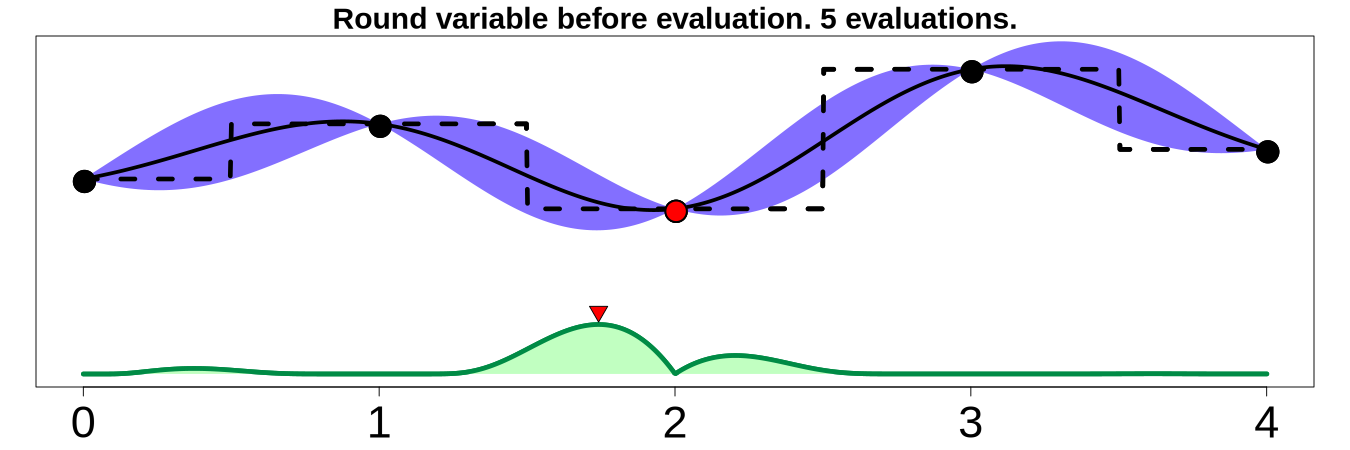
\includegraphics[width=0.475\linewidth]{integer/images/introduction/s5_before.pdf} \\
        \rotatebox{90}{\hspace{.7cm}{\bf \scriptsize Basic}} &
        \includegraphics[width=0.475\linewidth]{integer/images/introduction/s4_inside.pdf} &
        \includegraphics[width=0.475\linewidth]{integer/images/introduction/s5_inside.pdf} \\
        \rotatebox{90}{\hspace{.6cm}{\bf \scriptsize Proposed}} &
        \includegraphics[width=0.475\linewidth]{integer/images/introduction/s3_transform.pdf} &
        \includegraphics[width=0.475\linewidth]{integer/images/introduction/s5_transform.pdf} \\
\end{tabular}
\caption{{\small Different methods for dealing with integer-valued variables.
At the top of each image, we show a GP fit to the data (posterior mean and 1-std confidence interval, in purple)
that models a 1-dimensional objective taking values in the set $\{0,1,2,3,4\}$ (dashed line).
To display the objective we have rounded the real values at which to do the evaluation to the closest
integer. Below the GP fit, it is shown the acquisition function whose maximum is the recommendation for the next new
evaluation. Each column shows similar figures before and after evaluating a new point, respectively.
The proposed approach leads to no uncertainty about the objective after two evaluations.  Best seen in color.}}
\label{fig:methods}
\end{figure}

The previous problem can be easily solved. In the case of integer-valued variables, one can simply do 
the rounding to the closest integer value inside the wrapper that evaluates the objective. 
In the case of categorical variables, a similar approach can be followed inside the wrapper
using one-hot encoding. Namely, (i) look at which extra input variable has the largest
value, (ii) set that input variable equal to one, and (iii) set all other extra input variables equal to zero.
This basic approach is shown in the second row of Figure \ref{fig:methods} for the integer-valued case.
Here, the points at which the acquisition takes high values and the points at which the
objective is evaluated coincide. Thus, the BO method will tend to always perform evaluations at different input 
locations, as expected. This will avoid the problem described before, in which the BO method may get stuck.
The problem is, however, that the actual objective is constant in the intervals that are rounded to 
the same integer value. This constant behavior is ignored by the GP, which can lead to sub-optimal 
optimization results. The same behavior is expected in the case of categorical input variables.

\subsection{Proposed Approach} \label{sec:integer}

We propose here a method to alleviate the problems of the basic approach described in Section \ref{sec:dealing}. 
For this, we consider that the objective should be constant in those regions of the input space that
lead to the same input variable configuration on which the actual objective has to be evaluated. 
This property can be easily introduced into the GP by modifying the covariance function
$k(\cdot,\cdot)$. Covariance functions are often stationary and only depend on the distance between the 
input points \citep{rasmussen2003gaussian}. If the distance between two points is zero, the values of the function at 
both points will be the same (the correlation is equal to one). Based on this fact, we suggest to transform 
the input points to $k(\cdot,\cdot)$, obtaining an alternative covariance function $k'(\cdot,\cdot)$:
\begin{align}
k'(\mathbf{x}_i,\mathbf{x}_j) &= k(T(\mathbf{x}_i),T(\mathbf{x}_j)) \,,
\label{eq:covariance}
\end{align}
where $T(\mathbf{x})$ is a transformation in which all non real input variables of $f(\cdot)$ in $\mathbf{x}$ 
are modified as follows:
\begin{itemize}
\item The input variables corresponding to an integer-valued input variable are rounded to the closest integer value.
\item All extra input variables corresponding to the same categorical input variable are assigned zero value unless
	they take the largest value among the corresponding group of extra variables. If they take the largest value,
	they are assigned value one.
\end{itemize}
Essentially $T(\cdot)$ does the same transformation on $\mathbf{x}$ as the one described in Section
\ref{sec:basic_naive} for the basic approach inside the wrapper that evaluates the objective. Importantly, however, 
this transformation takes place in the covariance function of the GPs, which will allow for a 
better modeling of the objective. 

The beneficial properties of $k'(\cdot,\cdot)$ when used for BO are illustrated in the 
third row of Figure \ref{fig:methods} for the case of an integer-valued input variable. 
We can see that the GP model correctly identifies that the objective function is constant 
inside intervals of real values that are rounded to the same integer. The uncertainty is also 
the same in those intervals, and this is reflected in the acquisition function. Furthermore, after performing 
a single measurement in each interval, the uncertainty about $f(\cdot)$ goes to zero. This better modeling
of the objective is expected to be reflected in a better performance of the optimization process.
The same behavior is expected in the case of categorical variables.

In the case of integer-valued variables, the transformation $T(\mathbf{x})$ will round all integer-valued 
variables values in $\mathds{R}$ to the closest integer $k \in \mathds{Z}$. The set of integer values, 
$\mathds{Z}$, has a notion of order. That is, for all $z \in \mathbb{Z}$, we can define operators of order 
that involve two values: $<,>,\leq$ and $\geq$, such that $z_i < z_j$, $z_j > z_i$, $z_i \leq z_j$ and 
$z_j \geq z_i$, having that $z_i,z_j \in \mathbb{Z}$. This order will be preserved by the
resulting transformation. More precisely, assume an integer input variable and that $T(\mathbf{x})$ and $T(\mathbf{x}')$ 
only differ in the value of such integer input variable. The prior covariance between 
$f(\mathbf{x})$ and $f(\mathbf{x}')$ under $k(T(\mathbf{x}),T(\mathbf{x}'))$ will be higher the closer the 
corresponding integer values of $T(\mathbf{x})$ and $T(\mathbf{x}')$ are one from another. Therefore, the GP 
will be able to exploit the smoothness in the objective $f(\cdot)$ when solving the optimization problem.

In the case of categorical variables (\emph{e.g.}, variables that can take values such as 
\emph{red}, \emph{green}, \emph{blue}) there is no notion of order. That is, the operators 
$<,>,\geq$ and $\leq$ have no meaning nor purpose. One cannot compare two different 
values $c_1,c_2$ of any categorical-valued set $\mathds{C}$ according to these operators. However, 
what does exist in a categorical set is a notion of equality or difference, given by the operators $=,\neq$. 
The proposed transformation is able to preserve this notion of no order and notion of equal or 
different. More precisely, assume a single categorical variable and that $T(\mathbf{x})$ and $T(\mathbf{x}')$ 
only differ in the values of the corresponding extra variables associated to that categorical variable.
The prior covariance between $f(\mathbf{x})$ and $f(\mathbf{x}')$ under 
$k(T(\mathbf{x}),T(\mathbf{x}'))$ will be the same as long as $T(\mathbf{x})$ and $T(\mathbf{x}')$
encode a different value for the categorical variable. Of course if $T(\mathbf{x})$ and $T(\mathbf{x}')$
encode the same value for the categorical variable, the covariance will be maximum.

It is straight-forward to show that the proposed transformation generates a valid kernel function.
In particular, a kernel is valid if we can find an embedding $\phi(\cdot)$ such that $k(\mathbf{x},\mathbf{x}')=
\phi(\mathbf{x})^\text{T}\cdot \phi(\mathbf{x})$ \citep{shawe2004kernel}. Assume that the original kernel is valid
and hence $k(\mathbf{x},\mathbf{x}')= \phi(\mathbf{x})^\text{T}\cdot \phi(\mathbf{x})$ for some embedding $\phi(\cdot)$.
Then $k(T(\mathbf{x}),T(\mathbf{x}'))= \phi(T(\mathbf{x}))^\text{T}\cdot \phi(T(\mathbf{x}))$, and the  embedding
of the resulting kernel is simply given by $\phi(T(\cdot))$.

\subsubsection{Visualization of the Proposed Transformation} \label{sec:visual}

Figure \ref{fig:posterior} illustrates the modeling properties of the proposed transformation in the case of a real 
and an integer-valued variable (\ref{eq:covariance}). It shows the mean and standard deviation of the posterior 
distribution of a GP given some observations. It compares results with a standard GP that does not use the proposed 
transformation. In this case, the data has been sampled from a GP using the covariance function in (\ref{eq:covariance}) 
with $k(\cdot,\cdot)$ the squared exponential covariance function \citep{rasmussen2003gaussian}. One dimension takes continuous 
values and the other dimension takes values in $\{0,1,2,3,4\}$. Note that the posterior distribution captures the constant 
behavior of the function in any interval of values that are rounded to the same integer, only for the integer 
dimension (top). A standard GP (corresponding to the basic approach in Section \ref{sec:dealing}) cannot capture 
this shape (bottom).

Figure \ref{fig:posterior_categorical} illustrates the proposed transformation for the categorical case and a 
single variable that can only take two values, \emph{e.g.}, \emph{True} and \emph{False}. Using one-hot encoding,
these two values will be represented as $(0,1)$ and $(1,0)$, respectively. In the naive approach described before, this 
categorical variable will be replaced by two real variables taking values in the range $[0,1]$. Notwithstanding, any 
combination of values in which the first component is larger than the second will lead to the configuration value $(1,0)$.
Conversely, any combination of values in which the second component is larger will lead to the configuration value $(0,1)$.
Therefore, the corresponding objective will be constant in those regions of the input space that lead to the same configuration. 
This behavior is illustrated by Figure \ref{fig:posterior_categorical} (top), in which the posterior distribution of the GP is plotted 
given two observations. In this case we use the proposed transformation of the covariance function.
Note that the uncertainty goes to zero after just having a single observation corresponding to 
the \emph{True} value and a single observation corresponding to the \emph{False} value. This makes sense, because 
the objective is constant in all those regions of the input space that lead to the same configuration of 
the extra variables introduced in the input space. In Figure \ref{fig:posterior_categorical} (bottom) we show 
that a standard GP cannot model this behavior, and the posterior distribution of the mean is not constant in 
those regions of the input space that lead to the same configuration for the categorical variable. 
Furthermore, the posterior standard deviation is significantly different from zero, unlike in the proposed approach. 
Summing up, Figure \ref{fig:posterior_categorical} shows that by using the proposed covariance function, we are
better modeling the objective function, which in the end will be translated in better optimization results.



\begin{figure}[htb]
\begin{center}
\begin{tabular}{lcc}
	\rotatebox{90}{\hspace{1.75cm}{\bf \scriptsize Proposed Approach}} &  
        \includegraphics[width=0.375\linewidth]{integer/images/proposed_method/posterior_mean_persp3d_black.pdf} &
        \includegraphics[width=0.375\linewidth]{integer/images/proposed_method/posterior_std_dev_contour.pdf} \\
	\rotatebox{90}{\hspace{2.25cm}{\bf \scriptsize Standard GP}} &  
        \includegraphics[width=0.375\linewidth]{integer/images/proposed_method/posterior_mean_persp3d_black_real.pdf} &
        \includegraphics[width=0.375\linewidth]{integer/images/proposed_method/posterior_std_dev_contour_real.pdf} \\
\end{tabular}
\end{center}
\caption{{\small (top) Posterior mean and standard deviation of a GP model over a 2-dimensional space in which the first dimension
can only take $5$ different integer values and when the covariance function in (\ref{eq:covariance}) is used. Note that the second 
dimension can take any real value. (bottom) Same results for a GP model using a covariance function without the proposed
transformation.  Best seen in color.}}
\label{fig:posterior}
\end{figure}

\begin{figure}[htb]
\begin{center}
\begin{tabular}{lcc}
        \rotatebox{90}{\hspace{1.75cm}{\bf \scriptsize Proposed Approach}} &
        \includegraphics[width=0.375\linewidth]{integer/categorical/posterior_mean_perspective_categorical.pdf} &
        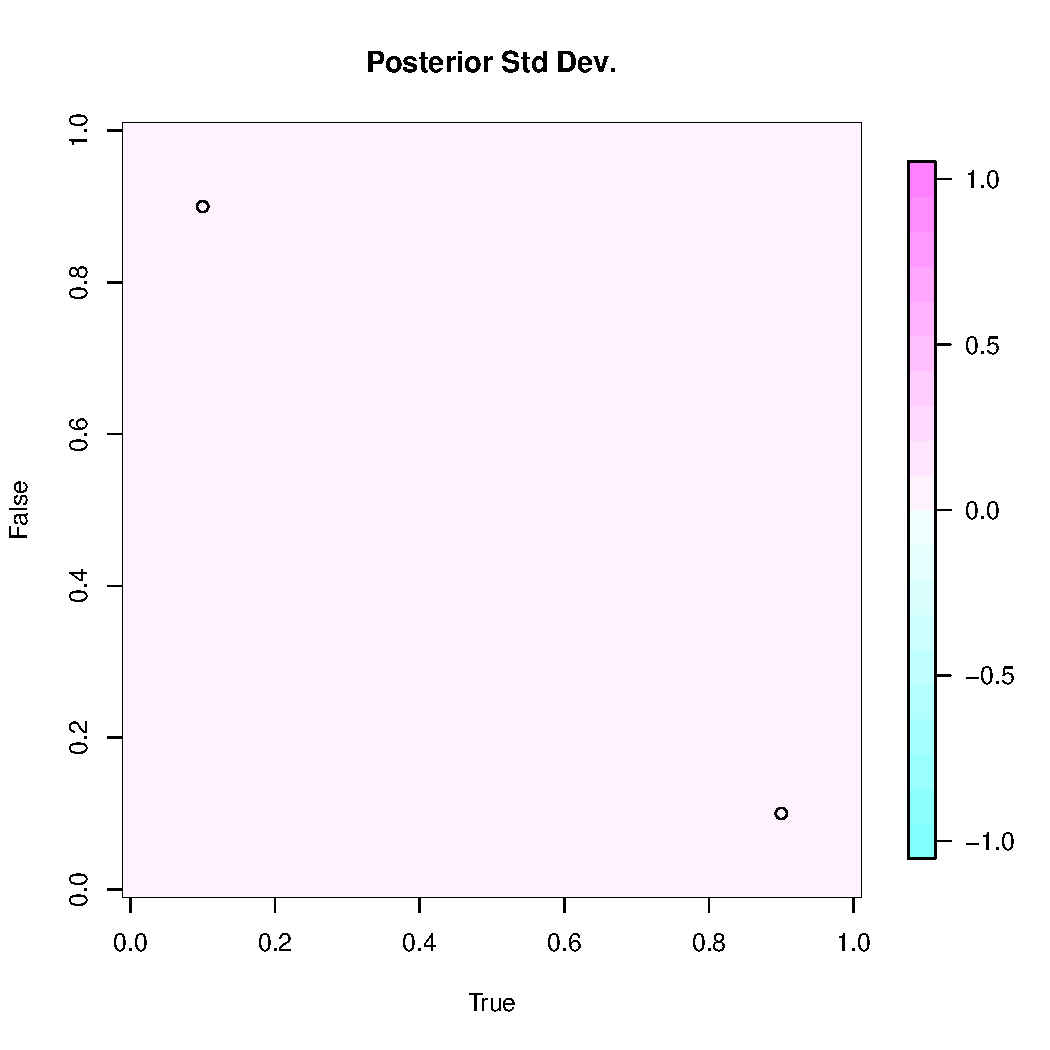
\includegraphics[width=0.375\linewidth]{integer/categorical/posterior_std_dev_contour_categorical.pdf} \\
        \rotatebox{90}{\hspace{2.25cm}{\bf \scriptsize Standard GP}} &
        \includegraphics[width=0.375\linewidth]{integer/categorical/posterior_mean_perspective_real.pdf} &
        \includegraphics[width=0.375\linewidth]{integer/categorical/posterior_std_dev_contour_real.pdf} \\
\end{tabular}
\end{center}
\caption{{\small (top) Posterior mean and standard deviation of a GP model over a 1-dimensional binary variable. 
The covariance function in (\ref{eq:covariance}) is used. Same results for a GP model using a covariance function without the proposed
transformation.  Best seen in color.}}
\label{fig:posterior_categorical}
\end{figure}

\subsection{Optimization of the Acquisition Function} \label{sec:acquisition}

A consequence of the transformation described in the previous section is that the
acquisition function will be flat in some regions of the input space, depending on the number of 
integer and categorical variables. This behavior is illustrated in Figure \ref{fig:methods} for one 
integer-valued variable. Often, the typical approach to optimize the acquisition is to evaluate it 
first on a grid of points to search for a good candidate point at which to start a gradient-based search 
using, \emph{e.g.}, L-BFGS. This is the approach employed by the BO software Spearmint. However, if the 
acquisition function is not smooth, this may be sub-optimal. Assume that we want to optimize a function 
with $D$ binary categorical inputs, with large $D$, for example, $30$. The best point after evaluating the 
acquisition function on a grid is extremely unlikely to be the best among the $2^D$ choices, and the 
gradient-based optimization of the acquisition function will not leave the starting point, since the 
acquisition function is expected to be flat at the starting point. 

To overcome this problem, we consider a block coordinate ascent optimization methodology which 
iterates between optimizing the non-real variables (integer-valued and categorical) and real variables,
similar to the one-exchange neighborhood (OEN) strategy described in \citep{hutter2009automated,levesque2017bayesian}.
Our methodology consists in using the grid and the L-BFGS methods to optimize all real 
variables and then, the OEN strategy to optimize the transformed integer and categorical variables. 
The OEN strategy is a greedy method. Under it, one iteratively evaluates for each non-real dimension, 
the corresponding neighbors of that dimension, and if some improvement is made in terms of the acquisition function, that new value is kept as the best 
one. This process is repeated until no further progress is made. Of course, to evaluate the quality of each neighbor, 
for a given integer-valued or categorical dimension, the real variables have to be optimized. For that task, we use the 
L-BFGS method. 

Of course, at this point one may ask whether the proposed transformation of the GP covariance function is beneficial
at all, and if simply optimizing the acquisition function as described here could be enough. To answer this question,
we have also implemented block coordinate ascent optimization methodology without transforming the integer-valued 
and categorical variables in the GP covariance function. We compared in a toy problem the results given by both approaches, 
the proposed approach and the alternating optimization methodology alone, which we refer to as OEN optimization only. 

Figure \ref{fig:comparison} shows the evaluations performed by the proposed approach and by OEN optimization only
in a 2-dimensional optimization problem with one real variable and one integer-valued variable taking 5 different values.
The contour curves show the value of the acquisition function. We show results after 10, 20 and 30 evaluations.
We observe that the proposed approach performs a more evenly evaluation of the input space. By contrast, the OEN 
optimization only strategy, which does not make use of the proposed transformation, tends to concentrate all 
evaluations in a particular region of the input space. This is a consequence of using a model (\emph{i.e.}, a GP 
without the proposed transformation) that ignores that the actual objective will take the same value in those regions 
of the input space that lead to the same integer value. In any case, our experiments of Section \ref{sec:experiments} 
show that OEN optimization only often performs better than the basic approach described in Section \ref{sec:dealing},
which simply uses a grid of points combined with L-BFGS to optimize the acquisition function with respect to all input variables,
independently of whether they take real, integer or categorical values.

\begin{figure}[htb]
\begin{center}
\begin{tabular}{lccc}
	& {\bf 10 evaluations} & {\bf 20 evaluations} & {\bf 30 evaluations} \\
	\rotatebox{90}{\hspace{0.5cm}{\bf \scriptsize OEN Opt. Only}} &
        \includegraphics[width=0.3\linewidth]{integer/toy/oen_1.pdf} &
        \includegraphics[width=0.3\linewidth]{integer/toy/oen_2.pdf} &
        \includegraphics[width=0.3\linewidth]{integer/toy/oen_3.pdf} \\
	\rotatebox{90}{\hspace{.1cm}{\bf \scriptsize Proposed Approach}} &
	\includegraphics[width=0.3\linewidth]{integer/toy/proposed_1.pdf} &
        \includegraphics[width=0.3\linewidth]{integer/toy/proposed_2.pdf} &
        \includegraphics[width=0.3\linewidth]{integer/toy/proposed_3.pdf} \\
\end{tabular}
\end{center}
\caption{{\small Evaluations plotted by crosses performed by the OEN optimization only 
method (top) and the proposed approach (bottom) of a 2-dimensional sample from a GP where 
one of the variables is integer-valued with range $5$. The contour represents the value of the 
acquisition function in the input space. From left to right, acquisition function with 10, 20 and 
30 evaluations. Best seen in color.}}
\label{fig:comparison}
\end{figure}

\section{Related Work} \label{sec:related}

We describe here two approaches that can be used as an 
alternative to BO methods using GPs when categorical and/or
integer-valued variables are present in a black-box optimization problem. These 
are Sequential model-based optimization for general algorithm configuration (SMAC) 
\citep{hutter2011sequential} and the Tree-structured Parzen Estimator Approach (TPE) 
\citep{bergstra2011algorithms}. Both can naturally handle integer and categorical-valued 
variables. SMAC is present in the popular machine learning tool AutoWeka \citep{thornton2013auto}. 
TPE is used in the HyperOpt tool \citep{bergstra2013hyperopt}.  

SMAC uses a random forest as the underlying surrogate model of the black-box 
objective \citep{breiman2001random}. The predictive distribution given by 
this model is used to select promising parameter values on which the objective should 
be evaluated. In random forest $T$ random regression trees are iteratively fit using 
each time a bootstrap sample of training data. Each bootstrap sample is obtained by drawing 
with replacement from the observed data $N$ instances. Furthermore, in random forest, at each node, 
a randomly chosen subset of variables are tested to split the data. This introduces variability in 
the generated regression trees. Given a candidate test location, the prediction for 
that point is computed for each of the $T$ trees. The predictive distribution of the model
is simply a Gaussian distribution with the empirical mean and variance across the individual
tree predictions. Given this predictive distribution, the EI criterion described in Section 
\ref{sec:back} is computed and used to select a new point at which the objective $f(\cdot)$ should 
be evaluated. The main advantage of random forest is that it has a smaller computational cost than
a GP. 

The regression trees used by random forest to compute the predictive 
distribution can naturally consider integer and categorical-valued variables.
Therefore this method does not suffer from the limitations described in Section \ref{sec:dealing}
for GPs. A problem, however, is that the predictive distribution of random forest is not 
very good. In particular, it relies on the randomness introduced by the bootstrap samples 
and the randomly chosen subset of variables to be tested at each node to split the data. 
This result is confirmed by our experiments, in which BO methods using GPs tend to 
perform better than SMAC.

In SMAC, the EI criterion is optimized by a simple multi-start local search algorithm. This method considers 
the ten resulting configurations with locally maximal EI from previous runs, and initiates a local search at each 
of them. To handle mixed categorical and integer parameter spaces, they use a randomized one-exchange 
neighbourhood search method. The search is stopped when none of the neighbours improves the EI criterion.
The configuration with the highest EI value is chosen as the candidate on which to evaluate the objective at 
the next iteration. More details on this method are given in \citep{hutter2011sequential}. 

TPE uses EI as the acquisition function. However, its computation is carried out in a 
different way, using a different modeling strategy. Whereas standard BO methods fit a 
discriminative model for $p(y|\mathbf{x})$ directly, TPE follows a generative approach. More 
precisely, $p(\mathbf{x}|y)$ and $p(y)$ are fit instead. Both approaches are related as 
$p(y|\mathbf{x}) = \frac{p(\mathbf{x}|y)p(y)}{p(\mathbf{x})}$ where $p(\mathbf{x}) = \int p(\mathbf{x}|y)p(y)dy$. 
To obtain an estimate of  $p(\mathbf{x}|y)$, TPE models each dimension with a probability distribution that serves 
as a prior for that dimension. Then, TPE replaces those distributions with non-parametric densities. 
TPE redefines $p(\mathbf{x}|y)$ by using two different densities, $\ell(\mathbf{x})$ and $g(\mathbf{x})$.
$\ell(\mathbf{x})$ is estimated using the observations in which the evaluation is lower than a 
chosen value $y^\star$. $g(\mathbf{x})$ is estimated using the rest of observations, respectively. That is,
\begin{align}
p(\mathbf{x}|y) & = \left\{ \begin{array}{cc}
	\ell(\mathbf{x}) & \text{if} \quad y \leq y^\star \,, \\
	g(\mathbf{x}) & \text{if} \quad y > y^\star \,.  
\end{array} \right.
\end{align}
Importantly, these two densities are obtained using Parzen estimators, a non-parametric density estimator, 
in the case of continuous random variables. In the case of  categorical
variables, a categorical distribution is used instead. Similarly, in the case of a variable over the integers,
a distribution that considers only this domain is used instead. This can easily account for categorical and integer-valued 
input variables in TPE. $y^\star$ is simply set as some quantile of the observed $y$ values. 
An interesting property of this approach is that no specific model for $p(y)$ is necessary. 
TPE derives a different expression for the EI acquisition function. Namely,
\begin{align}
\alpha(\mathbf{x}) & = \int_{-\infty}^{y^\star}(y^\star-y)p(y|\mathbf{x})dy  \nonumber \\
	& = \int_{-\infty}^{y^\star}
	(y^\star-y)\frac{p(\mathbf{x}|y)p(y)}{p(\mathbf{x})} dy \propto (\gamma + \frac{g(\mathbf{x})}{\ell(\mathbf{x})}(1-\gamma))^{-1}\,,
\end{align}
where we have used that $\gamma = p(y<y^\star)$ and that $p(\mathbf{x}) = \int p(\mathbf{x}|y)p(y)dy = \gamma l(\mathbf{x}) +
(1-\gamma)g(\mathbf{x})$. See \citep{bergstra2011algorithms} for further details.
Importantly, both of the models, $\ell(\mathbf{x})$ and $g(\mathbf{x})$, are 
hierarchical processes that naturally take into account discrete-valued and continuous-valued variables.

The TPE EI criterion is hence maximized simply by choosing points with high probability 
under $\ell(\mathbf{x})$ and low probability under $g(\mathbf{x})$. 
More precisely, in TPE, at each iteration, the evaluation is performed at the candiate point with greatest EI of many 
simulated points sampled from $\ell(\mathbf{x})$ and evaluated according to (proportionally) $\ell(\mathbf{x}) / g(\mathbf{x})$.
The particular form of $\ell(\mathbf{x})$ makes it easy to draw candidates with a mix between discrete and continous variables.

In the literature there are other approaches for BO with GPs that can account for categorical and 
integer-valued input variables. For example, \citep{rainforth2016bayesian,levesque2017bayesian} suggest to 
constrain the optimization of the acquisition function to consider only those values that are valid. This is 
essentially equivalent to the method OEN optimization only described in Section \ref{sec:acquisition}. This method 
is expected to give sub-optimal results for the reasons explained in that section.

A related approach to our proposed transformation to deal with categorical variables is the kernel proposed 
in \citep{hutter2009automated}. In that work it is used a weighted Hamming distance kernel to account for 
this type of variables. That method can be equivalent to our methodology when the squared exponential kernel is used. 
However, as we transform the inputs before feeding them into the kernel, our approach is more general and has the 
advantage of being able to use any valid kernel for GPs. More over, \citep{hutter2009automated} does not include any 
empirical evaluation of the benefits of considering such a kernel, nor it explains how to deal with integer-valued variables. 

\section{Experiments} \label{sec:experiments}

We carry out several experiments to evaluate the performance of our proposed approach for dealing with 
both integer and categorical-valued variables in Bayesian optimization. We compare the performance of this 
method with (i) the basic approach described in Section \ref{sec:dealing}. We also compare results with (ii) the 
basic approach that uses the OEN methodology for optimizing the acquisition function (without performing our 
suggested transformation in the covariance function of the GP). We refer to such a method as OEN optimization only. 
Each method has been implemented in the software for BO Spearmint in this branch (\url{https://github.com/EduardoGarrido90/Spearmint}).
Finally, we also compare results in both synthetic and real scenarios with two other methods that do not 
use GPs as the surrogate model. These methods are the ones described in the related work section. Namely, 
(iii) SMAC and (iv) TPE, as implemented in the HyperOpt platform.

In each experiment carried out in this section, we report average results and the corresponding
standard deviations. The results reported are averages over 100 repetitions of the corresponding experiment. 
Means and standard deviations are estimated using 200 bootstrap samples of the corresponding estimates. 
For the GPs we use a Mat\'ern covariance function and estimate 
the GP hyper-parameters using slice sampling \citep{murray2010}. The acquisition function that we employ in 
these experiments is PES.  The hyper-parameters of each GP
(length-scales, level of noise and amplitude) are approximately sampled from their posterior
distribution using slice sampling as in \cite{snoek2013}. We generate 10 samples for each
hyper-parameter, and the acquisition function of each method is averaged over these samples. In the real
world scenarios, we generate 50 samples for each hyper-parameter. For each method, at each iteration of the optimization 
process, we output a recommendation obtained by optimizing the GPs mean functions in the synthetic experiments. In the 
real-world experiments we return the best observation. Both SMAC and TPE deliver their recommendation
based on the best-observed evaluation in both synthetic and real-world scenarios.

The experiments contained in this section are organized as follows: The first set of experiments are synthetic and the
objective is sampled from a GP prior. Then, in order to compare GP Bayesian Optimization with non-GP Bayesian Optimization 
in scenarios where the function is not obtained from a GP, we consider three real optimization problems: Finding an optimal 
ensemble of trees on the digits dataset and finding an optimal deep neural network on the digits and MNIST datasets.

\subsection{Synthetic Experiments}

We compare the five methods described before when the objective is sampled from a GP prior. For this, we generate 
optimization problems involving 4 and 6  dimensions. We also consider two settings for each problem involving noisy and 
noiseless observations. The variance of the additive Gaussian noise is set equal to $0.01$ in the noisy setting.
In each problem the objective is randomly sampled from the corresponding GP prior 100 times and
we report average optimization results across the different samples. 

The first batch of experiments considers 4 input variables. The first 2 variables take real values and the 
rest of the variables take 4 and 3 different integer values, in the integer case. In the categorical case, the variables take 3 different categories. 
In the second batch of experiments we consider 6 input variables. The first 3 variables
take real values and the other 3 take 4, 3 and 2 different integer values, in the integer case, and 3 different 
categories, in the categorical case. The next section considers real, categorical and integer-variables at the same time.

In each setting, we sample the objective from a GP prior using (\ref{eq:covariance}) as the covariance function. 
Furthermore, we run each BO method (Basic, Proposed, OEN optimization only, SMAC and TPE) for 50 iterations in the 
4 inputs problem and for 100 iterations in the 6 inputs problem. For each method, we report the logarithm 
of the distance to the minimum value of each objective as a function of the evaluations done. In each of the 100 
random repetitions of the experiments we use a different random seed to generate the objective.

The average results of each method are displayed in Figure \ref{fig:results_synthetic_4} 
for the 4 input setting. We observe that the proposed approach gives better results than the other methods. 
In particular, it finds points that are closer to the optimal one with a smaller number of evaluations of the 
objective, both in the case of integer-valued (noiseless and noisy) and categorical-valued scenarios (noiseless and noisy). 
Figure \ref{fig:results_synthetic_6} shows similar results for the 6 input setting.


\begin{figure}[htb]
\begin{tabular}{cc}
        \includegraphics[width=0.475\linewidth]{integer/synthetic/noiseless/4Dif.pdf} &
        \includegraphics[width=0.475\linewidth]{integer/synthetic/noisy/4Dinf.pdf} \\
        \includegraphics[width=0.475\linewidth]{integer/synthetic/noiseless/4Dcf.pdf} & 
        \includegraphics[width=0.475\linewidth]{integer/synthetic/noisy/4Dcnf.pdf} \\
\end{tabular}
\caption{{\small Average results on the synthetic experiments with 4 dimensions.}}

\label{fig:results_synthetic_4}
\end{figure}

\begin{figure}[htb]
\begin{tabular}{cc}
	\includegraphics[width=0.475\linewidth]{integer/synthetic/noiseless/6Dif.pdf} &
        \includegraphics[width=0.475\linewidth]{integer/synthetic/noisy/6Dinf.pdf} \\
        \includegraphics[width=0.475\linewidth]{integer/synthetic/noiseless/6Dcf.pdf} &
        \includegraphics[width=0.475\linewidth]{integer/synthetic/noisy/6Dcnf.pdf} \\
\end{tabular}
\caption{{\small Average results on the synthetic experiments with 6 dimensions.}}
\label{fig:results_synthetic_6}
\end{figure}

We observe that GP based BO outperforms clearly the non-GP based BO, being the proposed approach better than the basic approach or 
the OEN optimization only method. This last method works better than the basic approach, showing that optimizing the acquisition 
function with the proposed methodology delivers better results.  In the 6-dimensional scenario the difference of performance between the 
basic approach, OEN optimization only and the proposed approach is slightly 
higher than in the 4-dimensional scenario. SMAC and TPE also perform worse than the other methods in the 6-dimensional 
case. Finally, in the noisy setting, the methods are more equal but the proposed approach works slightly better.
TPE and SMAC also deliver worse results in the noisy setting. 

Note that SMAC and TPE do not assume a GP for the underlying model and could be in disadvantage in these experiments. 
However, we believe it is still interesting to compare results with them in this setting in which the exact solution 
of the optimization problem can be easily obtained and the level of noise can be controlled. In the following section 
we carry out experiments in which the actual objectives need not be sampled from a GP, to illustrate the advantages 
of the proposed approach in a wider range of problems.

\subsection{Hyper-parameter Tuning of Machine Learning Algorithms}

We compare all methods on the practical problem of finding the optimal 
parameters of a gradient boosting ensemble \citep{friedman2001greedy} and a deep neural network on the digits dataset.
This dataset has 1,797 data instances, 10 class labels and 64 dimensions. It has been
extracted from the python package scikit-learn \citep{scikit-learn}.
Similarly, we also consider finding the optimal hyper-parameters of a deep neural network on 
the MNIST dataset \citep{lecun1998mnist}. This dataset has $60,000$ data instances, $768$ dimensions
and $10$ class labels. In this set of experiments, we use Predictive Entropy Search (PES) as 
the acquisition function, for both the basic, the proposed approach and the OEN optimization only method.

In the task of finding an optimal ensemble on the digits dataset, the objective that is considered for 
optimization is the average test log likelihood of the ensemble. This objective is evaluated using a 10-fold 
cross-validation procedure. Note that model bias can be an issue for all methods in this case, since the actual 
objective is unknown.  We consider a total of $200$ evaluations of the objective. A summary of the parameters optimized, 
their type and their range is displayed on Table \ref{table:6}. These parameters are: The logarithm of the learning rate, 
the maximum depth of the generated trees and the minimum number of samples used to split a node in the 
tree building process. Importantly, while the first parameter can take real values, the other two can only take integer values.

\begin{table}[htb]
\centering
\caption{Names, types and range of the parameters optimized for the ensemble of trees.}
\begin{tabular}{ l | c | c }
 \hline
 {\bf Name} & {\bf Type} & {\bf Range} \\
 \hline
 Log Learning Rate & Real & $[-10,0]$ \\
 Maximum Tree Depth & Integer & $[1,6]$ \\
 Minimum Number of Samples to Split & Integer & $[2,6]$ \\
 \hline
\end{tabular}
\label{table:6}
\end{table}

In each repetition of the experiment described (there are 100 repetitions) we consider a different 10-fold 
cross validation split of the data. The average results obtained are displayed in Figure \ref{fig:results_digits}.
This figure shows the average difference, in absolute value, between the test log-likelihood of the 
recommendation made and the best observed test-log likelihood, for that particular split, in a log scale. 
We observe that the proposed approach significantly outperforms the basic approach. More precisely, it is able
to find parameter values that lead to a gradient boosting ensemble with a better test log likelihood,
using a smaller number of evaluations of the objective. Furthermore, the proposed approach also performs
better than SMAC, TPE, or the OEN optimization only method.

\begin{figure}[htb]
        \begin{center}
        \includegraphics[width=0.7\linewidth]{integer/real/ensemble_digits_final_ok.pdf} \\
        \end{center}
\caption{{\small Average results on the Digits dataset using Gradient Boosting.}}
\label{fig:results_digits}
\end{figure}

In the task of finding an optimal deep neural network on the digits and MNIST dataset, the objective considered is 
the test log-likelihood of the network.  This objective is evaluated using a 10-fold cross-validation procedure in the 
digits dataset.  In the MNIST dataset a validation set of $10,000$ instances, extracted from the training set is used.
We consider $125$ and $150$ evaluations of the objective for the digits and the MNIST dataset, respectively. 
A summary of the parameters optimized, their type and their range is displayed on Table \ref{table:2}. These parameters 
are: The logarithm of the learning rate, the activation function and the number of hidden 
layers. The first parameter can take values in the real line. The second and third 
parameters are categorical and integer-valued. The number of units in each layer, is set
equal to $75$.

\begin{table}[htb]
\centering
\caption{Name, type and range of the deep neural network parameters optimized.}
\begin{tabular}{ c | c | c }
 \hline
 {\bf Name} & {\bf Type} & {\bf Range} \\
 \hline
 Log Learning Rate & Real & $[-10,0]$ \\
 Activation Function & Categorical & Linear, Sigmoid, Tanh or ReLU \\
 Number of hidden layers & Integer & $[1,3]$ \\
 \hline
\end{tabular}
\label{table:2}
\end{table}

The average results obtained in the two classification problems are displayed in Figure \ref{fig:results_deep}. 
The figure shows the average difference, in absolute value, between the test log-likelihood 
of the recommendation made and the best observed test-log likelihood, in a log scale. 
Again, the proposed approach significantly outperforms the basic approach. More precisely, it is able
to find parameter values that lead to a deep neural network with a better test log likelihood
on the left-out dataset, using a smaller number of evaluations of the objective. The proposed approach
also outperforms SMAC. However, on the MNIST dataset, TPE is only slightly worse than the proposed approach at 
the end and it outperforms the basic approach. We believe that the better results of TPE obtained in this 
problem can be a consequence of model bias in the GP that is used to fit the objective in the 
proposed approach. In both problems, the proposed approach outperforms the OEN optimization only method and the basic approach.

\begin{figure}[htb]
        \begin{center}
        \includegraphics[width=0.7\linewidth]{integer/real/rrnn_digits_final_ok.pdf} \\
        \includegraphics[width=0.7\linewidth]{integer/real/rrnn_final_ok.pdf} \\
        \end{center}
\caption{{\small Average results on the Digits and MNIST dataset using deep neural networks.}}
\label{fig:results_deep}
\end{figure}

\section{Conclusions} \label{sec:conclusions}

BO methods rely on a probabilistic model of the objective function, typically a Gaussian process (GP), 
upon which an acquisition function is built. The acquisition function is used to select candidate
points, on which the objective should be evaluated, to solve the optimization problem
in the smallest number of evaluations. Nevertheless, GPs assume continuous input variables. 
When this is not the case and some of the input variables take categorical or integer values, 
one has to introduce extra approximations. 
A common approach before doing the evaluation of the objective is to use a one-hot encoding 
approximation for categorical variables, or to round the value to the closest integer, in the case 
of integer-valued variables. We have shown that this can lead to problems
as the BO method can get stuck, always trying to evaluate the same candidate point. 

The problem described is a consequence of a mismatch between the regions of the input space that have high acquisition
values and the points on which the objective is evaluated. A simple way of avoiding this problem 
is to do the approximations (a one-hot encoding in the case of categorical
variables or the approximation to the closest integer in the case of integer-valued variables) inside the
wrapper that is used to evaluate the objective. This technique works in practice, but it has the limitation
that it makes the objective constant in those regions of the input space that lead to the same configuration.
This constant behavior cannot be modeled by standard GPs.

In this chapter we have proposed to modify the covariance function of the underlying GPs model to account for
those regions of the input space in which the objective should be constant. The transformation simply 
rounds integer-valued variables to the closest integer. In the case of categorical variables in which
one-hot encoding has been used, we simply set the largest extra variable equal to one and all the other equal to zero.
The consequence of this transformation is that the distance between those points of the input space 
that lead to the same configuration becomes zero. This enforces maximum
correlation between the GP values at those input values, leading to a constant behavior.

The proposed approach has been compared to a basic approach for dealing with categorical and integer-valued
input variables in the context BO and GPs. Furthermore, we have also compared results with two other approaches 
that can be used to solve these optimization problems and that can naturally account for integer and categorical
variables. Namely, SMAC and TPE. Several experiments involving synthetic and real-world experiments illustrate the 
benefits of the proposed approach. In particular, it outperforms the basic approach and SMAC and is most of the
times better or at least equivalent to TPE. 

The proposed approach also performs better than a strategy that constraints the optimization of the 
acquisition function to evaluate the objective only at those points that are feasible (\emph{i.e.}, 
the OEN optimization only method). Such a strategy partially solves the problems of doing a one-hot 
encoding approximation for categorical variables, or rounding the values to the closest integer, in the 
case of integer-valued variables. However, we show that it turns out to be sub-optimal in practice, since
the GP model considered ignores that the objective becomes constant in those regions of the input space
that lead to the same one-hot encoding or the same integer value.
 % Experiments

%\iclude{./Chapters/Chapter8} % Conclusions and Future Work

%% ----------------------------------------------------------------
% Now begin the Appendices, including them as separate files

\addtocontents{toc}{\vspace{2em}} % Add a gap in the Contents, for aesthetics

\appendix % Cue to tell LaTeX that the following 'chapters' are Appendices

% Appendix A

\chapter{Probability Distributions}
\label{AppendixA}
\lhead{Appendix \ref{AppendixA}. \emph{Fundamental Concepts of Probability Theory}}

In this appendix, we define some probability theory concepts that are used in the chapters of the thesis. We specifically describe the fundamentals of probability theory and some ideas of the Gaussian distribution. 

\section{Probability Theory}
Let $\mathbf{x} \in \mathbb{R}^N$. Let $X_1,...,X_N$ be $N$ random variables. The $d$-dimensional probability density function $p(X_1=x_1, \cdot \cdot \cdot, X_N=x_n)$ of the random variables $X_1,...,X_N$ with support in all $\mathbb{R}^N$ satisfies
\begin{equation}
\int_{\mathbb{R}^N} p(\mathbf{x}) d\mathbf{x} = 1\,.
\end{equation}
For clarity, we abbreviate the notation of probability density functions from $p(X_1=x_1, \cdot \cdot \cdot, X_N=x_n)$ to $p(\mathbf{x})$. If $p(\mathbf{x})$ is a probability density function of a $N$-dimensional real-valued space, then, its cumulative distribution function $F(x_l^{1} \leq X_1 \leq x_u^{1}, \cdot \cdot \cdot, x_l^{N} \leq X_N \leq x_u^{N})$ is given by:
\begin{equation}
F(x_l^{1} \leq X_1 \leq x_u^{1}, \cdot \cdot \cdot, x_l^{N} \leq X_N \leq x_u^{N})  = \int_{x_l^{1}}^{x_u^{1}} \cdot \cdot \cdot \int_{x_l^{N}}^{x_u^{N}} p(\mathbf{x}) d\mathbf{x}\,.
\end{equation}
For clarity, we abbreviate the notation of cumulative distribution functions from $F(x_l^{1} \leq X_1 \leq x_u^{1}, \cdot \cdot \cdot, x_l^{N} \leq X_N \leq x_u^{N})$ to $F(\mathbf{x})$. Let $X = (Y,Z) \in \mathbb{R}^2$ denote two random variables $Y \in \mathbb{R}, Z \in \mathbb{R}$ with a bivariate probability density function $p(\mathbf{x})$ on $\mathbb{R}^2$. Then, the marginal densities of $Y$ and $Z$ are given by the sum rule of probability:
\begin{align}
p(y) = \int_{\mathbb{R}} p(y, z) dz, \quad \quad p(z) = \int_{\mathbb{R}} p(y, z) dy.
\end{align}
This operation is also known as marginalization. It is usually performed to accumulate the uncertainty of the random variables that are not used for future computations. The conditional density $p(y|z)$, for $p(z) > 0$, is given by the product rule of probability:
\begin{align}
p(y|z) = \frac{p(y,z)}{p(z)}, \quad \quad p(y,z) = p(y|z) p(z) = p(z|y) p(y).
\label{eq:condit_prob}
\end{align}
Using Eq. (\ref{eq:condit_prob}), we can analytically obtain Bayes theorem:
\begin{align}
p(y|z) = \frac{P(z|y)P(y)}{P(z)}.
\end{align}
In Bayes theorem, we define $P(Z)$ as the model evidence, $P(y)$ is the prior distribution, $P(Z|Y)$ is the likelihood function and $P(Y|Z)$ is the posterior distribution. According to the total probability theorem, we have that the model evidence can be computed by the integral of the likelihood times the prior:
\begin{align}
P(z) = \int P(z|y)P(y) dy\,.
\end{align}
Let $z$ be substituted by observed data $\mathcal{D} = \{(\mathbf{x}_i, y_i)| i = 1,...,N\}$ where $N$ is the number of tuples $\mathbf{x}_i, y_i)$ and $y$ be the hyper-parameters $\boldsymbol{\theta}$ of a model $\mathcal{M}$. Bayes theorem can compute the posterior distribution of the hyper-parameters given the data $p(\boldsymbol{\theta}|\mathcal{D})$:
\begin{align}
p(\boldsymbol{\theta}|\mathcal{D}) = \frac{p(\mathcal{D}|\boldsymbol{\theta})p(\boldsymbol{\theta})}{p(\mathcal{D})}\,,
\end{align}
where the likelihood function $p(\mathcal{D}|\boldsymbol{\theta})$ is computed as the product of the likelihood function $p(y_i|\mathbf{x}_i, \boldsymbol{\theta})$ of each of the tuples $(\mathbf{x}_i, y_i)$ as:
\begin{align}
p(\mathcal{D}|\boldsymbol{\theta}) = \prod_{i=1}^{N} p(y_i|\mathbf{x}_i, \boldsymbol{\theta})\,.
\end{align}
$p(\boldsymbol{\theta})$ is the prior over the model hyper-parameters, that can be set as an uninformative prior or to some probability distribution given previous knowledge. Subjective bias is, from our opinion, always going to be present as, although we can set an uninformative prior for the weights, we are conditioning the posterior distribution given our subjective beliefs. We are setting an uninformative prior because we have the subjective belief that it is the best decision for the prior distribution. Hence, we are including a subjective bias in the computation. Finally, $p(\mathcal{D})$ is the model evidence. We can also rewrite Bayes theorem using the theorem of total probability as the following expression:
\begin{align}
p(\boldsymbol{\theta}|\mathcal{D}) = \frac{p(\mathcal{D}|\boldsymbol{\theta})p(\boldsymbol{\theta})}{\int p(\mathcal{D}|\boldsymbol{\theta})p(\boldsymbol{\theta}) d\boldsymbol{\theta}}\,.
\end{align}
Let $\boldsymbol{\Theta}$ be the space of hyper-parameter values. Let every possible value of the hyper-parameters $\boldsymbol{\theta} \in \boldsymbol{\Theta}$ be defined as a hypothesis that the model $\mathcal{M}$ can formulate about the data $\mathcal{D}$. The model evidence $p(\mathcal{D})$ represents the probability of the data given the model $\mathcal{M}$. In other words, how well does the model $\mathcal{M}$ fit the data $\mathcal{D}$ under every possible hypothesis $\boldsymbol{\theta}$ that can generate. It is used for Bayesian model selection. Models with higher marginal likelihood $p(\mathcal{D})$ explain the data better than those with lower marginal likelihood $p(\mathcal{D})$. The marginal likelihood $p(\mathcal{D})$ acts as normalization constant of the posterior distribution $p(\boldsymbol{\theta}|\mathcal{D})$. The posterior distribution $p(\boldsymbol{\theta}|\mathcal{D})$ of the hyper-parameters $\boldsymbol{\theta}$ given the data $\mathcal{D}$ represents all the possible hypotheses $\boldsymbol{\theta}$ of a model $\mathcal{M}$ weighted by their probability conditioned on data $\mathcal{D}$. We can update the posterior distribution $p(\boldsymbol{\theta}|\mathcal{D})$ of the hyper-parameters $\boldsymbol{\theta}$ given the data $\mathcal{D}$ every time that new data $\mathbf{x}_i, y_i)$ is available. New data incorporates a new likelihood function $p(y_i|\mathbf{x}_i, \boldsymbol{\theta})$ that affects the posterior distribution $p(\boldsymbol{\theta}|\mathcal{D})$. In a new iteration, we can state that the posterior $p(\boldsymbol{\theta}|\mathcal{D})$ becomes the new prior and the process is repeated. Hence, we can say that \textit{iudicium posterium discipulus est prioris} than translated means, the posterior is the student of the prior.

Finally, we can use the posterior distribution $p(\boldsymbol{\theta}|\mathcal{D})$ to make predictions with the model. Let $\mathbf{x}$ be a new data instance. We want to predict the value $y$ associated with the data instance $\mathbf{x}$. Let $y = f(\mathbf{x})$ be the unknown ground truth. A model $\mathcal{M}$ performs a prediction of the value $y$ associated with the data instance $\mathbf{x}$ given the observed data $\mathcal{D}$. As we can consider every possible hypothesis $\boldsymbol{\theta}$ that model $\mathcal{M}$ can compute of the data, we can compute a predictive distribtion $p(f(\mathbf{x})|\mathbf{x}, \mathcal{D})$ of the value $y$ associated with the data instance $\mathbf{x}$. The predictive distribution $p(f(\mathbf{x})|\mathbf{x}, \mathcal{D})$ can be seen as the pondered average of all the possible model predictions $p(f(\mathbf{x})|\mathbf{x}, \boldsymbol{\theta})$ times the probability of the model being configurated with the hyper-parameter values $\boldsymbol{\theta}$ given the data $\mathcal{D}$. This probability is computed with the posterior distribution $p(\boldsymbol{\theta}|\mathcal{D})$. Hence, the predictive distribution $p(f(\mathbf{x})|\mathbf{x}, \mathcal{D})$ can be computed as the product of $p(f(\mathbf{x})|\mathbf{x}, \boldsymbol{\theta})$ and $p(\boldsymbol{\theta}|\mathcal{D})$ marginalizing the model hyper-parameters $\boldsymbol{\theta}$:
\begin{equation}
p(f(\mathbf{x})|\mathbf{x}, \mathcal{D}) = \int p(f(\mathbf{x})|\mathbf{x}, \boldsymbol{\theta}) p(\boldsymbol{\theta}|\mathcal{D}) d\boldsymbol{\theta}\,.
\end{equation}
\section{Gaussian Distribution} \label{sec-appendix-Gaussian}
Let us first consider the case of univariate Gaussian distributions. Let $X$ be a random variable that is normally distributed. The associated probability density function $\mathcal{N}(x|\mu, \sigma)$ of the normally distributed random variable $X$ is parametrized by a mean $\mu$ and its standard deviation $\sigma$. The analytical expression of the probability density function associated to $X=x$ is:
\begin{align}
\mathcal{N}(x|\mu, \sigma) = \frac{1}{\sigma\sqrt{2\pi}}e^{-\frac{1}{2}(\frac{x-\mu}{\sigma})^2}\,.
\end{align}
The multivariate Gaussian distribution is the generalization of the univariate Gaussian distribution in the multi-dimensional scenario. Let $\mathbf{X} = [X_1,...,X_d]$ be a random variable vector. The multivariate Gaussian distribution corresponds to the joint probability density function of the vector of random variables. It is parametrized by a $d$-dimensional mean vector $\boldsymbol{\mu}$ and a positive semi-definite square covariance matrix $\boldsymbol{\Sigma}^{d \times d}$. The analytical expression of the probability density function associated to $\mathbf{X}=\mathbf{x}$ is:
\begin{align}
\mathcal{N}(\mathbf{x}|\bm{\mu}, \bm{\Sigma}) = \frac{1}{\sqrt{(2\pi)^d |\bm{\Sigma}|}} 
\exp \left\{ - \frac{1}{2} \left( \mathbf{x} - \bm{\mu} \right)^T \bm{\Sigma}^{-1} 
\left( \mathbf{x} - \bm{\mu} \right) \right\}\,, \label{eq:Appendix_Gaussian}
\end{align}
where the superscript $T$ means transpose. The analytical expression entropy $H[\mathcal{N}(x|\mu, \sigma)]$ of the univariate Gaussian distribution is:
\begin{align}
H[\mathcal{N}(x|\mu, \sigma)] = \frac{1}{2}\log(2\pi \text{e} \sigma^2)\,.
\end{align}
The entropy $H[\mathcal{N}(\mathbf{x}|\bm{\mu}, \bm{\Sigma})]$ of the multivariate Gaussian distribution is:
\begin{align}
H[\mathcal{N}(\mathbf{x}|\bm{\mu}, \bm{\Sigma})] = \frac{1}{2}\log[(2\pi \text{e})^d\bm{\Sigma}]\,.
\end{align}
The Gaussian distribution is an exponential family member. Exponential family is closed under product and division. Hence, both the multiplication and division operations are closed for multivariate Gaussian distributions. That is, the multiplication of two Gaussian distributions $\mathcal{N}(\mathbf{x}|\bm{\mu}_1,\bm{\Sigma}_1)$ and $\mathcal{N}(\mathbf{x}|\bm{\mu}_2,\bm{\Sigma}_2)$ is another Gaussian distribution $\mathcal{N}(\mathbf{x}|\bm{\mu},\bm{\Sigma})$. It is defined by the following expression, 
\begin{equation}
\mathcal{N}(\mathbf{x}|\bm{\mu}_1,\bm{\Sigma}_1) \mathcal{N}(\mathbf{x}|\bm{\mu}_2,\bm{\Sigma}_2) \propto \mathcal{N}(\mathbf{x}|\bm{\mu},\bm{\Sigma})\,,
\label{eq:Appendix_A_product_of_gaussians}
\end{equation}
where $\bm{\Sigma} = \left( \bm{\Sigma}_1^{-1} + \bm{\Sigma}_2^{-1} \right)^{-1}$ and $\bm{\mu} = \bm{\Sigma} \left(  \bm{\Sigma}_1^{-1} \bm{\mu}_1 + \bm{\Sigma}_2^{-1}\bm{\mu}_2 \right)$. The previous expression represents an unnormalized distribution. The normalization constant of $\mathcal{N}(\mathbf{x}|\bm{\mu},\bm{\Sigma})$ is given by the following expression:
\begin{equation}
Z = \sqrt{\frac{|\bm{\Sigma}|}{(2\pi)^d|\bm{\Sigma}_1||\bm{\Sigma}_2|}} 
\exp \left\{ -\frac{1}{2} \left( \bm{\mu}_1^T \bm{\Sigma}_1^{-1} \bm{\mu}_1 + 
\bm{\mu}_2^T \bm{\Sigma}_2^{-1} \bm{\mu}_2 - \bm{\mu}^T \bm{\Sigma}^{-1} \bm{\mu}  \right) \right\} \,,
\end{equation}
where $d$ is the dimensionality of the the Gaussian distribution. Regarding the division of two multivariate Gaussian distributions, we also have equivalent analytical expressions. In particular, the division of Gaussian distributions $\mathcal{N}(\mathbf{x}|\bm{\mu}_1,\bm{\Sigma}_1)$ and $\mathcal{N}(\mathbf{x}|\bm{\mu}_2,\bm{\Sigma}_2)$ is also another Gaussian distribution $\mathcal{N}(\mathbf{x}|\bm{\mu},\bm{\Sigma})$ which is given by the following analytical expression:
\begin{equation}
\mathcal{N}(\mathbf{x}|\bm{\mu}_1,\bm{\Sigma}_1) / \mathcal{N}(\mathbf{x}|\bm{\mu}_2,\bm{\Sigma}_2) \propto \mathcal{N}(\mathbf{x}|\bm{\mu},\bm{\Sigma})\,,
\label{eq:Appendix_A_quotient_of_gaussians}
\end{equation}
where $\bm{\Sigma} = \left( \bm{\Sigma}_1^{-1} - \bm{\Sigma}_2^{-1} \right)^{-1}$ and $\bm{\mu} = \bm{\Sigma} \left(\bm{\Sigma}_1^{-1} \bm{\mu}_1 - \bm{\Sigma}_2^{-1}\bm{\mu}_2 \right)$. As in the case of the product of two Gaussian distributions $\mathcal{N}(\mathbf{x}|\bm{\mu}_1,\bm{\Sigma}_1)$ and $\mathcal{N}(\mathbf{x}|\bm{\mu}_2,\bm{\Sigma}_2)$, we can also compute the normalization constant $Z$ of the unnormalized distribution $\mathcal{N}(\mathbf{x}|\bm{\mu},\bm{\Sigma})$. The normalization constant $Z$ can be computed via the following expression:
\begin{equation}
Z = \sqrt{\frac{(2\pi)^d|\bm{\Sigma}||\bm{\Sigma}_2|}{|\bm{\Sigma}_1|}} 
\exp \left\{ -\frac{1}{2} \left( \bm{\mu}_1^T \bm{\Sigma}_1^{-1} \bm{\mu}_1 - 
\bm{\mu}_2^T \bm{\Sigma}_2^{-1} \bm{\mu}_2 - \bm{\mu}^T \bm{\Sigma}^{-1} \bm{\mu}  \right) \right\} \,.
\end{equation}
The Gaussian distribution is an exponential family member. Therefore, the Gaussian distribution $\mathcal{N}(\mathbf{x}|\bm{\mu}, \bm{\Sigma})$ can be rewritten as an exponential family representation via the following expression:
\begin{equation}
\mathcal{N}(\mathbf{x}|\bm{\mu}, \bm{\Sigma}) = \exp (\bm{\eta}^T \mathbf{u}(\mathbf{x}) - g(\bm{\eta}))\,,
\end{equation}
where $\bm{\eta}$ is a vector of natural parameters, $\mathbf{u}(\mathbf{x})$ is a vector function of $\mathbf{x}$ known as the sufficient statistics and $g(\bm{\eta})$ is the cumulant generating function or log partition function. The log partition function $g(\bm{\eta})$ guarantees that $\exp (\bm{\eta}^T \mathbf{u}(\mathbf{x}) - g(\bm{\eta}))$ integrates to $1$. We can compute the sufficient statistics $\mathbf{u}(\mathbf{x})$ and the log partition function $g(\bm{\eta})$ via the following expressions for the particular case of the Gaussian distribution $\mathcal{N}(\mathbf{x}|\bm{\mu}, \bm{\Sigma})$:
\begin{align}
\mathbf{u}(\mathbf{x}) & = \left( x_1,\ldots,x_d, \right.  & \bm{\eta} & =  - \frac{1}{2} \left( -2 \bm{\mu}^T \bm{\Sigma}^{-1} \right.,  \nonumber \\
& \quad x_1^2, x_1 x_2, \ldots, x_1 x_d, && \quad \Sigma^{-1}_{11}, \Sigma^{-1}_{12}, \ldots, \Sigma^{-1}_{1d}, \nonumber \\ 
& \quad x_1 x_2, x_2^2, \ldots, x_2 x_d, && \quad \Sigma^{-1}_{21}, \Sigma^{-1}_{22}, \ldots, \Sigma^{-1}_{1d},\nonumber \\
& \quad \quad \vdots && \quad \quad \vdots \nonumber \\
& \quad \left. x_d x_1, x_d x_2, \ldots, x_d^2 \right)^T\,, && \quad \left. 
\Sigma^{-1}_{d1}, \Sigma^{-1}_{d2},\ldots, \Sigma^{-1}_{dd} \right)^T
\end{align}
and $g(\bm{\eta}) = \frac{1}{2} \bm{\mu}^T \bm{\Sigma}^{-1} \bm{\mu} + \frac{d}{2}\log(2\pi) + \frac{1}{2} \log(|\bm{\Sigma}|)$. Let us consider an univariate Gaussian distribution $\mathcal{N}(x|\mu_g, \sigma_g)$. We can transform the parameters $\mu_g$ and $\sigma_g$ of a Gaussian distribution $\mathcal{N}(x|\mu_g, \sigma_g)$ into its natural parameters $\mu_n$ and $\sigma_n$ using the following expressions:
\begin{align}
\mu_n = \frac{\mu_g}{\sigma_g} \,, \\
\sigma_n = \frac{1}{\sigma_g} \,.
\end{align}
We can also deconvert the natural parameters, $\mu_n$ and $\sigma_n$, into the Gaussian ones, $\mu_g$ and $\sigma_g$, using the following expressions:
\begin{align}
\sigma_g = \frac{1}{\sigma_n} \,, \\
\mu_g = \mu_n \sigma_g \,.
\end{align}
Let us now consider a joint Gaussian distribution $\mathcal{N}(\boldsymbol{\mu}_n, \boldsymbol{\sigma}_n \text{I})$ where $\text{I}$ is the identity matrix. This distribution factorizes as a product of univariate independent Gaussian distributions $\mathcal{N}(\boldsymbol{\mu}_n, \boldsymbol{\sigma}_n \text{I}) = \prod_{i=1}^{N} \mathcal{N}(\mu_n, \sigma_n)$.  We can convert the parameters of this joint distribution $\mathcal{N}(\boldsymbol{\mu}_n, \boldsymbol{\sigma}_n \text{I})$ using the following analytical expression:
\begin{align}
\boldsymbol{\mu}_n = \frac{\boldsymbol{\mu}_g}{diag(\boldsymbol{\sigma}_g)} \,, \\
\boldsymbol{\sigma}_n = \frac{1}{diag(\boldsymbol{\sigma}_g)}\,.
\end{align}
We can also deconvert the natural parameters, $\boldsymbol{\mu}_n$ and $\boldsymbol{\sigma}_n$, into the Gaussian ones, $\boldsymbol{\mu}_g$ and $\boldsymbol{\sigma}_g$, using the following expressions:
\begin{align}
\boldsymbol{\sigma}_g = \frac{1}{\boldsymbol{\sigma}_n} \,, \\
\boldsymbol{\mu}_g = \boldsymbol{\mu}_n \boldsymbol{\sigma}_g \,.
\end{align}
Transforming the Gaussian parameters, $\boldsymbol{\mu}_g$ and $\boldsymbol{\sigma}_g$, into the natural ones, $\boldsymbol{\mu}_n$ and $\boldsymbol{\sigma}_n$, is interesting as the expressions for the product and division of Gaussian distributions become simpler. Let us return to the case of the univariate Gaussian distribution. The product of two Gaussian distributions $\mathcal{N}(\mu_{n1}, \sigma_{n1})$ and $\mathcal{N}(\mu_{n2}, \sigma_{n2})$ with natural parameters $\mu_{n1}, \sigma_{n1}$ and $\mu_{n2}, \sigma_{n2}$ is a Gaussian distribution $\mathcal{N}(\mu_{n3}, \sigma_{n3})$ with parameters $\mu_{n3}, \sigma_{n3}$. The parameters $\mu_{n3}, \sigma_{n3}$ are given by the addition of the parameters of the two distributions $\mathcal{N}(\mu_{n1}, \sigma_{n1})$ and $\mathcal{N}(\mu_{n2}, \sigma_{n2})$ that are being multiplied:
\begin{align}
\mu_{n3} = \mu_{n1} + \mu_{n2} \,, \\
\sigma_{n3} = \sigma_{n1} + \sigma_{n2} \,.
\end{align}
Similarly, the division of two Gaussian distributions $\mathcal{N}(\mu_{n1}, \sigma_{n1})$ and $\mathcal{N}(\mu_{n2}, \sigma_{n2})$ with natural parameters, $\mu_{n1}, \sigma_{n1}$ and $\mu_{n2}, \sigma_{n2}$, is a Gaussian distribution $\mathcal{N}(\mu_{n3}, \sigma_{n3})$ where its natural parameters $\mu_{n3}, \sigma_{n3}$ are given by the substraction of the two distributions $\mathcal{N}(\mu_{n1}, \sigma_{n1})$ and $\mathcal{N}(\mu_{n2}, \sigma_{n2})$ that are being divided:
\begin{align}
\mu_{g3} = \mu_{g1} - \mu_{g2} \,, \\
\sigma_{g3} = \sigma_{g1} - \sigma_{g2} \,.
\end{align}
Let us consider now a multivariate Gaussian distribution $\mathcal{N}(\boldsymbol{\mu}_g, \boldsymbol{\Sigma}_g)$ with parameters $\boldsymbol{\mu}_g, \boldsymbol{\Sigma}_g$. We can compute its natural parameters $\boldsymbol{\mu}_n, \boldsymbol{\Sigma}_n$ using the following expressions:
\begin{align}
\boldsymbol{\mu}_n = \boldsymbol{\Sigma}_g^{-1} \boldsymbol{\mu}_g \,, \\
\boldsymbol{\Sigma}_n = \boldsymbol{\Sigma}_g^{-1} \,.
\end{align}
As in the case of univariate distributions, we can reconvert the natural parameters into the Gaussian ones using the following expression:
\begin{align}
\boldsymbol{\Sigma}_g = (\boldsymbol{\Sigma}_n)^{-1} \,, \\
\boldsymbol{\mu}_g = \boldsymbol{\Sigma}_g \boldsymbol{\mu}_n \,. 
\end{align}
Consider two multivariate Gaussian distributions $\mathcal{N}(\boldsymbol{\mu}_1, \boldsymbol{\Sigma}_1)$ and $\mathcal{N}(\boldsymbol{\mu}_2, \boldsymbol{\Sigma}_2)$ with natural parameters $\boldsymbol{\mu}_1, \boldsymbol{\Sigma}_1$ and $\boldsymbol{\mu}_2, \boldsymbol{\Sigma}_2$. The product of two Gaussian distributions $\mathcal{N}(\boldsymbol{\mu}_1, \boldsymbol{\Sigma}_1)$ and $\mathcal{N}(\boldsymbol{\mu}_2, \boldsymbol{\Sigma}_2)$ is another Gaussian distribution $\mathcal{N}(\boldsymbol{\mu}_3, \boldsymbol{\Sigma}_3)$ with natural parameters $\boldsymbol{\mu}_3, \boldsymbol{\Sigma}_3$ such that $\boldsymbol{\mu}_3, \boldsymbol{\Sigma}_3$ are given by:
\begin{align}
\boldsymbol{\mu}_3 = \boldsymbol{\mu}_1 + \boldsymbol{\mu}_2\,, \\
\boldsymbol{\Sigma}_3 = \boldsymbol{\Sigma}_1 + \boldsymbol{\Sigma}_2 \,.
\end{align}
Consider two multivariate Gaussian distributions $\mathcal{N}(\boldsymbol{\mu}_1, \boldsymbol{\Sigma}_1)$ and $\mathcal{N}(\boldsymbol{\mu}_2, \boldsymbol{\Sigma}_2)$ with natural parameters $\boldsymbol{\mu}_1, \boldsymbol{\Sigma}_1$ and $\boldsymbol{\mu}_2, \boldsymbol{\Sigma}_2$. The division of two Gaussian distributions $\mathcal{N}(\boldsymbol{\mu}_1, \boldsymbol{\Sigma}_1)$ and $\mathcal{N}(\boldsymbol{\mu}_2, \boldsymbol{\Sigma}_2)$ is another Gaussian distribution $\mathcal{N}(\boldsymbol{\mu}_3, \boldsymbol{\Sigma}_3)$ with natural parameters $\boldsymbol{\mu}_3, \boldsymbol{\Sigma}_3$ such that $\boldsymbol{\mu}_3, \boldsymbol{\Sigma}_3$ are given by:
\begin{align}
\boldsymbol{\mu}_3 = \boldsymbol{\mu}_1 - \boldsymbol{\mu}_2\,, \\
\boldsymbol{\Sigma}_3 = \boldsymbol{\Sigma}_1 - \boldsymbol{\Sigma}_2 \,.
\end{align}
Let $\mathcal{N}(\mathbf{x}|\bm{\mu},\bm{\Sigma})$
and $\mathcal{N}(\mathbf{y}|\bm{\mu}',\bm{\Sigma}')$ be two multivariate Gaussian distributions. The Kullback-Leibler (KL) divergence between $\mathcal{N}(\mathbf{x}|\bm{\mu},\bm{\Sigma})$ and $\mathcal{N}(\mathbf{y}|\bm{\mu}',\bm{\Sigma}')$ is
\begin{equation}
\text{KL}\left(\mathcal{N}(\mathbf{x}|\bm{\mu},\bm{\Sigma}),\mathcal{N}(\mathbf{y}|\bm{\mu}',\bm{\Sigma}')\right)  = \frac{1}{2} \left( \frac{|\bm{\Sigma}'|}{|\bm{\Sigma}|} \right) + 
\text{trace} \left( \bm{\Sigma}'^{-1} \bm{\Sigma} - \mathbf{I} \right) + 
(\bm{\mu}'-\bm{\mu})^T \bm{\Sigma}'^{-1} (\bm{\mu}'-\bm{\mu})\,. \label{eq:Appendix_KL_Gaussian}
\end{equation}
The moments of two Gaussian distributions $\mathcal{N}(\mathbf{x}|\bm{\mu},\bm{\Sigma})$ and $\mathcal{N}(\mathbf{y}|\bm{\mu}',\bm{\Sigma}')$ are matched if $\text{KL}\left(\mathcal{N}(\mathbf{x}|\bm{\mu},\bm{\Sigma}),\mathcal{N}(\mathbf{y}|\bm{\mu}',\bm{\Sigma}')\right) = 0$. Let $p(\mathbf{x})$ be an unnormalized probability distribution, the normalization constant $Z$ of $p(\mathbf{x})$ is given by: 
\begin{align}
Z = \int p(\mathbf{x}) d\mathbf{x}
\end{align}
Let $t(\mathbf{x})$ be an arbitrary function of $\mathbf{x}$ and let
\begin{align}
Z & = \int t(\mathbf{x}) \mathcal{N}(\mathbf{x}|\bm{\mu},\bm{\Sigma}) d \mathbf{x}\,, &
p(\mathbf{x}) & = \frac{1}{Z} t(\mathbf{x}) \mathcal{N}(\mathbf{x}|\bm{\mu},\bm{\Sigma})\,.
\label{eq:Z_exp}
\end{align}
In this case, $p(\mathbf{x})$ is a probability distribution, as it has been normalized by the constant $Z$. The first and second moments of a multivariate Gaussian distribution $\mathcal{N}(\mathbf{x}|\bm{\mu}, \bm{\Sigma})$ are given by the following expressions:
\begin{align}
\mathbb{E}[\mathbf{x}] & = \boldsymbol{\mu}\,,\\
\mathbb{E}[\mathbf{x}\mathbf{x}^T] & = \boldsymbol{\Sigma} + \boldsymbol{\mu}\boldsymbol{\mu}^T\,.
\end{align}
The first and second moments of two distributions can be matched via the following expressions: 
\begin{align}
\mathds{E}_{p}[\mathbf{x}]  & = \bm{\mu} + \bm{\Sigma} \frac{\partial  \log(Z)}{\partial \bm{\mu}} \,, 
\label{eq:AppendixA_new_mean}\\
\mathds{E}_{p}[\mathbf{x}\mathbf{x}^T] - 
\mathds{E}_{p}[\mathbf{x}] \mathds{E}_{p}[\mathbf{x}]^T
&  = \bm{\Sigma} - \bm{\Sigma}\left(\frac{\partial  \log(Z)}{\partial \bm{\mu}} 
\left(\frac{\partial  \log(Z)}{\partial \bm{\mu}}\right)^T  - 2 \frac{\partial \log(Z)}{\partial \bm{\Sigma}} \right) \bm{\Sigma} \,.
\label{eq:AppendixA_new_var}
\end{align}
In some practical situations, $\partial \log(Z) / \partial \boldsymbol{\Sigma}$ is not robust. In that cases, we can use the second derivative of the mean, $\partial^2 \log (Z) / \partial (\boldsymbol{\mu})^2$, rather than $\partial \log(Z) / \partial \boldsymbol{\Sigma}$. By doing it so, Eq. (\ref{eq:AppendixA_new_var1}) is now given by the following expression:
\begin{equation}
\mathds{E}_{p(\mathbf{x})}[\mathbf{x}\mathbf{x}^T] - \mathds{E}_{p(\mathbf{x})}[\mathbf{x}] \mathds{E}_{p(\mathbf{x})}[\mathbf{x}]^T
 = \boldsymbol{\Sigma} \frac{\partial^2 \log (Z)}{\partial (\boldsymbol{\mu})^2} \boldsymbol{\Sigma} + \boldsymbol{\Sigma}\,.
\label{eq:z2ok}
\end{equation}
Let the normalization constant of a distribution, $Z$, be defined by Eq. (\ref{eq:Z_exp}). Let $\boldsymbol{\mu}$ and $\boldsymbol{\Sigma}$ be the mean and covariance of the multivariate Gaussian distribution that appears in Eq. (\ref{eq:Z_exp}) multiplying the factor $t(\mathbf{x})$. Let $\partial \log (Z)/\partial \boldsymbol{\mu}$ be the derivative of $Z$ with respect to $\boldsymbol{\mu}$. Finally, let $\mathcal{N}(\mathbf{x}|\bm{\mu}, \bm{\Sigma})$ be:
\begin{align}
\mathcal{N}(\mathbf{x}|\bm{\mu}, \bm{\Sigma}) = \frac{1}{\sqrt{(2\pi)^d |\bm{\Sigma}|}} 
\exp \left\{ - \frac{1}{2} \left( \mathbf{x} - \bm{\mu} \right)^T \bm{\Sigma}^{-1} 
\left( \mathbf{x} - \bm{\mu} \right) \right\}\,. \label{eq:Appendix_Gaussian}
\end{align}
Then, we can infer Eq. (\ref{eq:z2ok}) from the following expressions. First, we compute the first derivative, $\partial \log (Z)/\partial \boldsymbol{\mu}$:
\begin{align}
&  \frac{\partial \log (Z)}{\partial (\boldsymbol{\mu})} = \frac{1}{Z} \frac{\partial Z}{\partial \boldsymbol{\mu}} \nonumber \,, \\
& \frac{\partial Z}{\partial \boldsymbol{\mu}} = \int t(\mathbf{x}) \mathcal{N}(\mathbf{x}|\boldsymbol{\mu}, \boldsymbol{\Sigma}) (-0.5) 2 (\mathbf{x} - \boldsymbol{\mu})^T \boldsymbol{\Sigma}^{-1} (-1) d \mathbf{x} \nonumber \,, \\
& \frac{\partial Z}{\partial \boldsymbol{\mu}} = \int t(\mathbf{x}) \mathcal{N}(\mathbf{x}|\boldsymbol{\mu}, \boldsymbol{\Sigma}) (\mathbf{x} - \boldsymbol{\mu})^T \boldsymbol{\Sigma}^{-1} d \mathbf{x} \nonumber \,, \\
& \frac{\partial \log (Z)}{\partial (\boldsymbol{\mu})} = \frac{1}{Z} \int t(\mathbf{x}) \mathcal{N}(\mathbf{x}|\boldsymbol{\mu}, \boldsymbol{\Sigma}) (\mathbf{x} - \boldsymbol{\mu})^T \boldsymbol{\Sigma}^{-1} d \mathbf{x} \,. 
\end{align}
Then, we can compute the second derivative, $\partial^2 \log (Z)/\partial (\boldsymbol{\mu})^2$. We need to know that $\mathds{E}_{p(\mathbf{x})}[\mathbf{x}] = \int t(\mathbf{x}) N(\mathbf{x}|\boldsymbol{\mu},\boldsymbol{\Sigma}) \mathbf{x} d \mathbf{x}$:
\begin{align}
& \frac{\partial^2 \log (Z)}{\partial (\boldsymbol{\mu})^2} = \frac{\partial 1/Z}{\partial \boldsymbol{\mu}} \int t(\mathbf{x}) \mathcal{N}(\mathbf{x}|\boldsymbol{\mu},\boldsymbol{\Sigma})(\mathbf{x} - \boldsymbol{\mu}) \boldsymbol{\Sigma}^{-1} d \mathbf{x} + \nonumber \\ & \frac{1}{Z} \frac{\partial \int t(\mathbf{x}) \mathcal{N}(\mathbf{x}|\boldsymbol{\mu},\boldsymbol{\Sigma}) (\mathbf{x} - \boldsymbol{\mu})^T \boldsymbol{\Sigma}^{-1} d \mathbf{x}}{\partial{\boldsymbol{\mu}}} \nonumber \,, \\
& \frac{\partial 1/Z}{\partial \boldsymbol{\mu}} = - \frac{1}{Z^2} \frac{\partial Z}{\partial \boldsymbol{\mu}}  = - \frac{1}{Z^2}  \int t(\mathbf{x}) \mathcal{N}(\mathbf{x}|\boldsymbol{\mu},\boldsymbol{\Sigma})  (\mathbf{x} - \boldsymbol{\mu})^T  \boldsymbol{\Sigma}^{-1}  d \mathbf{x} \nonumber \,, \\
& \frac{\partial \int t(\mathbf{x}) \mathcal{N}(\mathbf{x}|\boldsymbol{\mu},\boldsymbol{\Sigma})  (\mathbf{x} - \boldsymbol{\mu})^T  \boldsymbol{\Sigma}^{-1}  d\mathbf{x}}{ \partial \boldsymbol{\mu}} = \int t(\mathbf{x}) \mathcal{N}(\mathbf{x}|\boldsymbol{\mu},\boldsymbol{\Sigma})  \boldsymbol{\Sigma}^{-1} (\mathbf{x} - \boldsymbol{\mu}) (\mathbf{x} - \boldsymbol{\mu})^T  \boldsymbol{\Sigma}^{-1}  d\mathbf{x} - \nonumber \\ 
& \int t(\mathbf{x}) \mathcal{N}(\mathbf{x}|\boldsymbol{\mu},\boldsymbol{\Sigma})  \boldsymbol{\Sigma}^{-1} d\mathbf{x} \nonumber \,, \\
& \frac{\partial^2 \log (Z)}{\partial \boldsymbol{\mu}^2} = - \frac{1}{Z^2}  \int t(\mathbf{x}) \mathcal{N}(\mathbf{x}|\boldsymbol{\mu},\boldsymbol{\Sigma})  (\mathbf{x} - \boldsymbol{\mu})^T  \boldsymbol{\Sigma}^{-1}  d\mathbf{x}  \int t(\mathbf{x}) \mathcal{N}(\mathbf{x}|\boldsymbol{\mu},\boldsymbol{\Sigma})  (\mathbf{x} - \boldsymbol{\mu})  \boldsymbol{\Sigma}^{-1}  d\mathbf{x} + \nonumber \\ 
& \frac{1}{Z}  [ \int t(\mathbf{x}) \mathcal{N}(\mathbf{x}|\boldsymbol{\mu},\boldsymbol{\Sigma})  \boldsymbol{\Sigma}^{-1} (\mathbf{x} - \boldsymbol{\mu}) (\mathbf{x} - \boldsymbol{\mu})^T  \boldsymbol{\Sigma}^{-1}  d\mathbf{x} - \int t(\mathbf{x}) \mathcal{N}(\mathbf{x}|\boldsymbol{\mu},\boldsymbol{\Sigma})  \boldsymbol{\Sigma}^{-1} d\mathbf{x} ] \nonumber \,, \\
& \frac{\partial^2 \log (Z)}{\partial \boldsymbol{\mu}^2} = - \frac{1}{Z^2}  [ \int t(\mathbf{x}) \mathcal{N}(\mathbf{x}|\boldsymbol{\mu},\boldsymbol{\Sigma})  \boldsymbol{\Sigma}^{-1} (\mathbf{x} - \boldsymbol{\mu})  d\mathbf{x}]   [\int t(\mathbf{x}) \mathcal{N}(\mathbf{x}|\boldsymbol{\mu},\boldsymbol{\Sigma})  (\mathbf{x} - \boldsymbol{\mu})^T  \boldsymbol{\Sigma}^{-1}  d\mathbf{x}] + \nonumber \\
& \frac{1}{Z}  [ \int t(\mathbf{x}) \mathcal{N}(\mathbf{x}|\boldsymbol{\mu},\boldsymbol{\Sigma})  \boldsymbol{\Sigma}^{-1} [ \mathbf{x} \mathbf{x}^T - 2 \boldsymbol{\mu} \mathbf{x}^T  + \boldsymbol{\mu} \boldsymbol{\mu}^T ]  \boldsymbol{\Sigma}^{-1}  d \mathbf{x} - \int t(\mathbf{x}) \mathcal{N}(\mathbf{x}|\boldsymbol{\mu},\boldsymbol{\Sigma})  \boldsymbol{\Sigma}^{-1} d \mathbf{x} ] \nonumber \,, \\
& \frac{\partial^2 \log (Z)}{\partial \boldsymbol{\mu}^2} = - \frac{1}{Z}  [ \int t(\mathbf{x}) \mathcal{N}(\mathbf{x}|\boldsymbol{\mu},\boldsymbol{\Sigma})  \boldsymbol{\Sigma}^{-1} (\mathbf{x} - \boldsymbol{\mu})  d\mathbf{x}]  \frac{1}{Z}  [\int t(\mathbf{x}) \mathcal{N}(\mathbf{x}|\boldsymbol{\mu},\boldsymbol{\Sigma})  (\mathbf{x} - \boldsymbol{\mu})^T  \boldsymbol{\Sigma}^{-1}  d\mathbf{x}] + \nonumber \\
& \frac{1}{Z}  [ \int t(\mathbf{x}) \mathcal{N}(\mathbf{x}|\boldsymbol{\mu},\boldsymbol{\Sigma})  \boldsymbol{\Sigma}^{-1} [ \mathbf{x} \mathbf{x}^T - 2 \boldsymbol{\mu} \mathbf{x}^T  + \boldsymbol{\mu} \boldsymbol{\mu}^T ]  \boldsymbol{\Sigma}^{-1}  d \mathbf{x} - \int t(\mathbf{x}) \mathcal{N}(\mathbf{x}|\boldsymbol{\mu},\boldsymbol{\Sigma})  \boldsymbol{\Sigma}^{-1} d\mathbf{x} ] \nonumber \,, \\
& \frac{\partial^2 \log (Z)}{\partial \boldsymbol{\mu}^2} = - \boldsymbol{\Sigma}^{-1} [ \mathds{E}_{p(\mathbf{x})}[\mathbf{x}] - \boldsymbol{\mu}  ]^T  [ \mathds{E}_{p(\mathbf{x})}[\mathbf{x}] - \boldsymbol{\mu}  ] \boldsymbol{\Sigma}^{-1} + \nonumber \\ 
& \frac{1}{Z}  [ \int t(\mathbf{x}) \mathcal{N}(\mathbf{x}|\boldsymbol{\mu},\boldsymbol{\Sigma})  \boldsymbol{\Sigma}^{-1} [ \mathbf{x} \mathbf{x}^T - 2 \boldsymbol{\mu} \mathbf{x}^T  + \boldsymbol{\mu} \boldsymbol{\mu}^T ]  \boldsymbol{\Sigma}^{-1}  d \mathbf{x} - \int t(\mathbf{x}) \mathcal{N}(\mathbf{x}|\boldsymbol{\mu},\boldsymbol{\Sigma})  \boldsymbol{\Sigma}^{-1} d \mathbf{x} ] \nonumber \,, \\
& \frac{\partial^2 \log (Z)}{\partial \boldsymbol{\mu}^2} = - \boldsymbol{\Sigma}^{-1} [ \mathds{E}_{p(\mathbf{x})}[\mathbf{x}] - \boldsymbol{\mu}  ]^T  [ \mathds{E}_{p(\mathbf{x})}[\mathbf{x}] - \boldsymbol{\mu}  ] \boldsymbol{\Sigma}^{-1} + \nonumber \\
& \frac{1}{Z}  [ \int t(\mathbf{x}) \mathcal{N}(\mathbf{x}|\boldsymbol{\mu},\boldsymbol{\Sigma})  \boldsymbol{\Sigma}^{-1} [ \mathbf{x} \mathbf{x}^T - 2 \boldsymbol{\mu} \mathbf{x}^T  + \boldsymbol{\mu} \boldsymbol{\mu}^T ]  \boldsymbol{\Sigma}^{-1}  d \mathbf{x}]  - \boldsymbol{\Sigma}^{-1} \nonumber \,, \\
\end{align}
where the derivation continues as follows,
\begin{align}
\frac{\partial^2 \log (Z)}{\partial \boldsymbol{\mu}^2} & = - \boldsymbol{\Sigma}^{-1} [ \mathds{E}_{p(\mathbf{x})}[\mathbf{x}] - \boldsymbol{\mu}  ]  [ \mathds{E}_{p(\mathbf{x})}[\mathbf{x}] - \boldsymbol{\mu}  ]^T \boldsymbol{\Sigma}^{-1} + \nonumber \\ & \boldsymbol{\Sigma}^{-1} [ \mathds{E}_{p(\mathbf{x})}[\mathbf{x}\mathbf{x}^T] - 2 \boldsymbol{\mu} \mathds{E}_{p(\mathbf{x})}[\mathbf{x}]^T  + \boldsymbol{\mu} \boldsymbol{\mu}^T ]  \boldsymbol{\Sigma}^{-1}  - \boldsymbol{\Sigma}^{-1} \nonumber \,, \\
& = \boldsymbol{\Sigma}^{-1} [- [ \mathds{E}_{p(\mathbf{x})}[\mathbf{x}] - \boldsymbol{\mu}  ]  [ \mathds{E}_{p(\mathbf{x})}[\mathbf{x}] - \boldsymbol{\mu}  ]^T + \nonumber \\ & [ \mathds{E}_{p(\mathbf{x})}[\mathbf{x}\mathbf{x}^T] - 2 \boldsymbol{\mu} \mathds{E}_{p(\mathbf{x})}[\mathbf{x}]^T  + \boldsymbol{\mu} \boldsymbol{\mu}^T ] ] \boldsymbol{\Sigma}^{-1} - \boldsymbol{\Sigma}^{-1} \nonumber \,, \\
& = \boldsymbol{\Sigma}^{-1} [- [ \mathds{E}_{p(\mathbf{x})}[\mathbf{x}] - \boldsymbol{\mu}  ]  [ \mathds{E}_{p(\mathbf{x})}[\mathbf{x}] - \boldsymbol{\mu}  ]^T + \nonumber \\ & [ \mathds{E}_{p(\mathbf{x})}[\mathbf{x}\mathbf{x}^T] - 2 \boldsymbol{\mu} \mathds{E}_{p(\mathbf{x})}[\mathbf{x}]^T  + \boldsymbol{\mu} \boldsymbol{\mu}^T ] - \boldsymbol{\Sigma} ] \boldsymbol{\Sigma}^{-1} \nonumber \,, \\
&  = \boldsymbol{\Sigma}^{-1} [ - \mathds{E}_{p(\mathbf{x})}[\mathbf{x}] \mathds{E}_{p(\mathbf{x})}[\mathbf{x}]^T + 2  \boldsymbol{\mu}  \mathds{E}_{p(\mathbf{x})}[\mathbf{x}]^T - \nonumber \\ & \boldsymbol{\mu}\boldsymbol{\mu}^T + [\mathds{E}_{p(\mathbf{x})}[\mathbf{x}\mathbf{x}^T] - 2 \boldsymbol{\mu} \mathds{E}_{p(\mathbf{x})}[\mathbf{x}]^T  + \boldsymbol{\mu} \boldsymbol{\mu}^T ] - \boldsymbol{\Sigma} ] \boldsymbol{\Sigma}^{-1} \nonumber \,, \\
& = \boldsymbol{\Sigma}^{-1} [ - \mathds{E}_{p(\mathbf{x})}[\mathbf{x}] \mathds{E}_{p(\mathbf{x})}[\mathbf{x}]^T + \mathds{E}_{p(\mathbf{x})}[\mathbf{x}\mathbf{x}^T] - \boldsymbol{\Sigma} ] \boldsymbol{\Sigma}^{-1} \nonumber \,, \\
& = \boldsymbol{\Sigma}^{-1} [ \mathds{E}_{p(\mathbf{x})}[\mathbf{x}\mathbf{x}^T] - \mathds{E}_{p(\mathbf{x})}[\mathbf{x}] \mathds{E}_{p(\mathbf{x})}[\mathbf{x}]^T - \boldsymbol{\Sigma} ] \boldsymbol{\Sigma}^{-1} \nonumber \,, \\
\end{align}
where we see that we can finally substitute $\mathds{E}_{p(\mathbf{x})}[\mathbf{x}\mathbf{x}^T] - \mathds{E}_{p(\mathbf{x})}[\mathbf{x}] \mathds{E}_{p(\mathbf{x})}[\mathbf{x}]^T$ by:
\begin{align}
\boldsymbol{\Sigma} \frac{\partial^2 \log (Z)}{\partial \boldsymbol{\mu}^2} \boldsymbol{\Sigma} =  \mathds{E}_{p(\mathbf{x})}[\mathbf{x}\mathbf{x}^T] - \mathds{E}_{p(\mathbf{x})}[\mathbf{x}] \mathds{E}_{p(\mathbf{x})}[\mathbf{x}]^T - \boldsymbol{\Sigma}  \nonumber \,, \\
\mathds{E}_{p(\mathbf{x})}[\mathbf{x}\mathbf{x}^T] - \mathds{E}_{p(\mathbf{x})}[\mathbf{x}] \mathds{E}_{p(\mathbf{x})}[\mathbf{x}]^T =  \boldsymbol{\Sigma} \frac{\partial^2 \log (Z)}{\partial \boldsymbol{\mu}^2} \boldsymbol{\Sigma} + \boldsymbol{\Sigma} \,. 
\end{align}
	% Multi-Task Datasets

%% Appendix B

\chapter{Appendix for Chapter \ref{Chapter4}}
\label{AppendixB}
\lhead{Appendix \ref{AppendixB}. \emph{Appendix for Chapter \ref{Chapter4}}}

We provide, in this Appendix, additional material that complements the exposition of the PESMOC approach introduced in Chapter \ref{Chapter4}. Concretely, we show the exact computations done by the expectation propagation algorithm to approximate the intractable factors of the conditional predictive distribution involved in the PESMOC acquisition function approximation. We also include a sensitivity analysis of the number of Monte Carlo iterations of the Slice sampling algorithm. Additionaly, we include another sensitivity analysis of the sampled Pareto sets and an analysis of the infeasible solutions in benchmark experiments.


\section{Vector-Valued Reproducing Kernel Hilbert Spaces}%Single-Task Learning with \acrshort{mtl} Kernels}
To give different definitions of vector-valued kernels, we will follow the work of~\citet{MicchelliP05}.
Consider $\Yspace$ a Hilbert space with inner product $\ydotp{.}{.}$, and $\mathcal{L}(\Yspace)$ the space of linear operators from $\Yspace$ to $\Yspace$; then we can study the Hilbert spaces $\hilbertspace$ of functions
\begin{equation*}
    \begin{aligned}
        f: &  & \Xspace &  &  & \to &  &  &  & \Yspace &  & \\
           &  & x       &  &  & \to &  &  &  & f(x)    &  &
    \end{aligned}
\end{equation*}
with inner product $\dotp{\cdot}{\cdot}$.
The kernels in such spaces are operator-valued functions $K: \Xspace \times \Xspace \to \mathcal{L}(\Yspace)$.
We look at these spaces from three different and equivalent perspectives: continuous evaluation functionals, positive-definite kernels and feature maps.

%\paragraph*{Continuous evaluation functionals.}
The first approach considered is that of continuous evaluation functionals.
% Given a Hilbert space with continuous evaluation functionals, which are defined later, we can find the reproducing kernel operator.
Consider the vector-valued Hilbert space $\mathcal{H}$ with inner product $\dotp{\cdot}{\cdot}$ of functions defined in $\Xspace$ and values in $\Yspace$, and the functionals
%$L_{x, y} f = \ydotp{y}{f(x)}$,
\begin{equation*}
    \begin{aligned}
        L_{x, y}: &  & \hilbertspace &  & \to &  &  & \Yspace &  &  & \to &  &  & \reals          &  & \\
                  &  & f             &  & \to &  &  & f(x)    &  &  & \to &  &  & \ydotp{y}{f(x)} &  &
    \end{aligned}.
\end{equation*}
If these functionals are continuous, we can apply Riesz representation theorem~\citep{riesz2012functional}. That is, for every $x \in \Xspace, y \in \Yspace$ we can find an unique $g_{x, y} \in \hilbertspace$ such that for all $f \in \hilbertspace$,
\begin{equation}\label{eq:vector_riesz}
    L_{x, y} f = \ydotp{y}{f(x)} = \dotp{g_{x,y}}{f}_{\hilbertspace} .
\end{equation}
We can now give the definition of vector-valued Hilbert space from the point of view of continuous functionals as in~\citet[Definition 2.1]{MicchelliP05}.
\begin{definition}[vector-valued RKHS]
    We say that $\hilbertspace$ is a vector-valued RKHS when for any $x \in \Xspace$ and $y \in \Yspace$, the functional $L_{x, y} f = \ydotp{y}{f(x)}$ is continuous.
\end{definition}
Note that this is a definition similar to the scalar case but we use the inner product of $\Yspace$ to construct the scalar-valued functionals $L_{x, y}$. The price we pay is that it is necessary to express the Riesz representation as dependent of the elements $y \in \Yspace$. To get rid of this dependence, for every $x \in \Xspace$ we can define the linear operator
\begin{equation}
    \label{eq:vector_riesz}
    \begin{aligned}
        g_x: &  & \Yspace &  &  & \to &  &  &       & \hilbertspace &  & \\
             &  & y       &  &  & \to &  &  & g_x y & = g_{x, y}    &  &
    \end{aligned}.
\end{equation}
This operator is well defined because $g_{x, y}$ is unique for every $x \in \Xspace, y \in \Yspace$ and its linearity is easy to check from the linearity of the inner product $\ydotp{.}{.}$.
%
Using these results, we can now define the operator
\begin{equation}\label{eq:vector_kernel}
    \begin{aligned}
        K(x, \hat{x}) : &  & \Yspace &  &  & \to &  &  &                 & \Yspace               &  & \\
                        &  & y       &  &  & \to &  &  & K(x, \hat{x}) y & = (g_{\hat{x}} y) (x) &  &
    \end{aligned}
\end{equation}
for every $x, \hat{x} \in \Xspace$.
%Observe that $K(x, \hat{x})$ is linear since $\forall x,\;  g_x$ is linear, i.e. $g_x(\lambda_1 y_1 + \lambda_2 y_2) = \lambda_1 g_x(y_1) + \lambda_2 g_x(y_2)$.
It is possible then to prove that $K(x, \hat{x})$ is a reproducing kernel in $\mathcal{H}$ as seen in~\citet[Propositon 2.1]{MicchelliP05}.

\begin{proposition}
    If $K(x, \tilde{x})$ is defined for every $x, \hat{x} \in \Xspace$ as in ~\eqref{eq:vector_kernel} and $g_x$ is defined as in ~\eqref{eq:vector_riesz}, then
    \begin{equation}
        \nonumber
        K: \Xspace \times \Xspace \to \mathcal{L}(\Yspace)
    \end{equation}
    is a kernel that for every $x, \hat{x} \in \Xspace$ satisfies:
    \begin{enumerate}
        \item For every $y, \hat{y} \in \Yspace$, we have
              \begin{equation}
                  \nonumber
                  \ydotp{y}{K(x, \tilde{x}) \hat{y}} = \dotp{g_x \hat{y}}{g_{\hat{x}} y} .
              \end{equation}
        \item $K(x, \tilde{x}) = \adj{K(\tilde{x}, x)}$ and $K(x, x)$ is positive definite for every $x \in \Xspace$.
        \item Given $n \in \naturals$, for any  $x_1, \ldots, x_n \in \Xspace,  y_1, \ldots, y_n \in \Yspace$,
              \begin{equation}
                  \nonumber
                  \sum_{i, j =1}^n \ydotp{y_i}{K(x_i, x_j) y_j} \geq 0.
              \end{equation}
        \item $\norm{g_x} = \norm{K(x, x)}^{\frac{1}{2}}$.
        \item $\norm{K(x, t)} \leq \norm{K(x, x)}^{\frac{1}{2}} \norm{K(t, t)}^{\frac{1}{2}}$.
        \item For every $f \in \hypspace$ and $x \in \Xspace$, we have that
              $$ \norm{f(x)} \leq \norm{f} \norm{K(x, x)}^{\frac{1}{2}} .$$
    \end{enumerate}
\end{proposition}

% To do that, first we have to define a vector-valued kernel and the corresponding reproducing property.
% \begin{definition}[operator-valued Kernel]
%     Given a non-empty set $\Xspace$, if $\Yspace$ is a finite-dimensional Hilbert space
%     % , and $\hilbertspace$ is a Hilbert space of $\Yspace$-valued functions with domain in $\Xspace$
%      an operator-valued kernel is a function
%     \begin{equation}
%         \nonumber
%         K: \Xspace \times \Xspace \to \mathcal{L}(\Yspace)
%     \end{equation}
%     which is symmetric and positive definite.
% \end{definition}
% For the clarity of the text an operator-valued $K$ will be referred just as a kernel unless an explicit distinction is needed.
% \begin{definition}[Reproducing Property of operator-valued operators]
%     If $\Yspace$ is a finite-dimensional Hilbert space, and $\hilbertspace$ is a Hilbert space of $\Yspace$-valued functions with domain in $\Xspace$, a function
%     \begin{equation}
%         \nonumber
%         K: \Xspace \times \Xspace \to \mathcal{L}(\Yspace)
%     \end{equation}
%     has the reproducing property if $\forall x \in \Xspace, y \in \Yspace, \forall f \in \hilbertspace,$ 
%     $$ \ydotp{y}{f(x)} = \dotp{K(\cdot, x) y}{f}_\hilbertspace.$$ 
% \end{definition}
% A kernel with the reproducing property is also called a reproducing kernel. The next proposition shows how we can build a reproducing kernel for a space $\hilbertspace$ in which the evaluation functionals are continuous.
% \begin{proposition}
%     If for every $x, \hat{x} \in \Xspace$, the function $K(x, \hat{x})$ is defined as in Equation~\eqref{eq:vector_kernel}, then the function
%     \begin{equation}
%         \nonumber
%         K: \Xspace \times \Xspace \to \mathcal{L}(\Yspace)
%     \end{equation}
%     is a reproducing kernel.
% \end{proposition}
% \begin{proof}
%     To prove that $K$ is a reproducing kernel we need to check: 
%     \begin{enumerate}
%         \item\label{item:vvkernel_bounded} $K(x, \hat{x})$ is bounded for every $x, \hat{x} \in \Xspace$ so $K$ is well defined.
%         \item\label{item:vvkernel_symmetric} $K$ is symmetric: $\adj{K(x, \hat{x})} = K(\hat{x}, x)$, where $\adj{A} \in \mathcal{L}(\Yspace)$ is the adjoint of $A \in \mathcal{L}(\Yspace)$.
%         \item\label{item:vvkernel_positive}  $K$ is positive definite: given $n \in \naturals$, for any  $x_1, \ldots, x_n \in \Xspace,  y_1, \ldots, y_n \in \Yspace$,
%         \begin{equation}
%             \nonumber
%             \sum_{i, j =1}^n \ydotp{y_i}{K(x_i, x_j) y_j} \geq 0.
%         \end{equation}
%         \item\label{item:vvkernel_repr} It has the reproducing property: $\forall x \in \Xspace, y \in \Yspace, \forall f \in \hilbertspace,$ $ \ydotp{y}{f(x)} = \dotp{K(\cdot, x) y}{f}.$
%     \end{enumerate}
%     To prove~\ref{item:vvkernel_bounded} and~\ref{item:vvkernel_symmetric}, observe that by
%     applying~\eqref{eq:vector_riesz} to $f = g_{\hat{x}}\hat{y}$, for every $x \in \Xspace, y \in \Yspace$ there exists an unique $g_{x, y} = g_{x}y$ such that
%     \begin{equation}
%         \ydotp{y}{(g_{\hat{x}} \hat{y}) (x)} = \dotp{g_{x}y}{g_{\hat{x}}\hat{y}} ,
%     \end{equation}
%     and combining this result with~\eqref{eq:vector_kernel} we get
%     \begin{equation}
%         \nonumber
%         \ydotp{y}{K(x, \hat{x}) \hat{y}} = \ydotp{y}{(g_{\hat{x}} \hat{y})(x) }= \dotp{g_{x}y}{g_{\hat{x}}\hat{y}}.
%     \end{equation}
%     Also, using the definitions,
%     \begin{equation}
%         \nonumber
%         \ydotp{K(\hat{x}, x) y}{ \hat{y}} = \ydotp{(g_{x} y)(\hat{x})}{\hat{y}} = \ydotp{\hat{y}}{(g_{x} y)(\hat{x})} = \dotp{g_{\hat{x}} \hat{y}}{g_x y}.
%     \end{equation}
%     Since both operators $K(x, \hat{x}), K(\hat{x}, x)$ are bilinear, by the Uniform Boundness Principle~\citep{Akhiezer1961TheoryOL}, $K(x, \hat{x}), K(\hat{x}, x)$ are bounded (hence continuous) and $K(x, \hat{x})^* = K(\hat{x}, x)$.
%     \\
%     To prove~\ref{item:vvkernel_positive} we write
%     \begin{equation}
%         \nonumber
%         \sum_{i, j =1}^n \ydotp{y_i}{K(x_i, x_j) y_j} = \sum_{i, j =1}^n \dotp{g_{x_i} y_i}{g_{x_j} y_j}  = \norm{\sum_{i=1}^n g_{x_i} y_i}^2 \geq 0 .
%     \end{equation}
%     Finally, to prove~\ref{item:vvkernel_repr} we use that 
%     $\forall x \in \Xspace, y \in \Yspace, \forall f \in \hilbertspace, \exists g_{x, y} \in \hilbertspace$ such that 
%     $$ \ydotp{y}{f(x)} = \dotp{g_{x, y}}{f} = \dotp{g_{x} y}{f} =\dotp{K(\cdot, x) y}{f}.$$
% \end{proof}

%\paragraph*{Positive semi-definite kernels.}
The second approach of~\citet{MicchelliP05} to define vector-valued kernels changes the point of view. Given a kernel $K$, the Hilbert space from which $K$ is the reproducing kernel is built.
To do this, we use~\citet[Theorem 2.1]{MicchelliP05}, which extends the Moore-Aronszanj Theorem:
\begin{theorem}\label{th:moore-arons_vector}
    If $K: \Xspace \times \Xspace \to \mathcal{L}(\Yspace)$ is a kernel, then there exists a unique (up to an isometry) RKHS which admits $K$ as its reproducing kernel.
\end{theorem}
The proof is similar to that of the Moore-Aronszanj Theorem, considering the space of the completion of the span of $\left\lbrace K_x = K(\cdot, x) , x \in \Xspace \right\rbrace$.

%\paragraph*{Feature map.}
The last approach is based on feature maps, which provide a very simple way of generating kernels.
\begin{lemma}
    Given some Hilbert space $\mathcal{W}$, any continuous feature map $\Phi: \Xspace \to \mathcal{L}(\mathcal{W}, \mathcal{Y})$ defines a kernel as
    \begin{equation}
        \label{eq:kernel_featmap}
        K(x, \hat{x}) = \Phi(x) \circ \adj{\Phi(\hat{x})}: \Yspace \to \Yspace .
    \end{equation}
\end{lemma}
\begin{proof} We need to prove that it is bounded, symmetric and positive definite:
    \begin{enumerate}
        \item Since $\Phi(x)$ is continuous, its adjoint $\adj{\Phi(x)}$ is continuous and the composition $\Phi(x) \circ \adj{\Phi(\hat{x})}$ is also continuous.
        \item It is symmetric since  $\adj{(\Phi(x) \circ \adj{\Phi(\hat{x})})} = (\adj{(\adj{\Phi(x)})} \circ \adj{\Phi(\hat{x})}) = (\Phi(x) \circ \adj{\Phi(\hat{x})}) $.
        \item It is semipositive definite since, given any $x_1, \ldots, x_n \in \Xspace,  y_1, \ldots, y_n \in \Yspace$
              \begin{equation}
                  \nonumber
                  \begin{aligned}
                      \sum_{i, j =1}^n \ydotp{y_i}{K(x_i, x_j) y_j} & = \sum_{i, j =1}^n \ydotp{y_i}{ \Phi(x_i) \circ \adj{\Phi(x_j)} y_j}                                                      \\
                                                                    & = \sum_{i, j =1}^n \ydotp{\adj{\Phi(x_i)} y_i}{ \adj{\Phi(x_j)} y_j} = \norm{\sum_{i=1}^n \adj{\Phi(x_i)} y_i}^2 \geq 0 .
                  \end{aligned}
              \end{equation}
    \end{enumerate}
\end{proof}
% Since $K$ as defined in~\eqref{eq:kernel_featmap} is a kernel, according to Theorem~\ref{th:moore-arons_vector} we can find its corresponding vector-valued Hilbert space $\hilbertspace$.

%\subsubsection*{Representer Theorem for Operator-Valued Kernels}
These definitions related to vector-valued \acrshort{rkhss} are useful to get a better understanding of how to apply operator-valued kernels for learning multi-target or multi-task functions. Concretely, we would like to develop some result similar to representer theorem~\cite{ScholkopfHS01}, which is a crucial result in optimization and \acrshort{ml}. Given a regularized empirical risk, under some assumptions, the theorem gives a precise description of the minimizer $f^*$ as a finite linear combination of functions $K(\cdot, x_i)$ where $x_i$ are part of the empirical sample.
This result is extended in~\citet[Theorem 4.2]{MicchelliP05} for operator-valued kernels through the next theorem.
\begin{theorem}
    Let $\mathcal{Y}$ be a Hilbert space and let $\mathcal{H}$ be the Hilbert space of $\mathcal{Y}$-valued functions with an operator-valued reproducing kernel $K$. Let $V: \Yspace^n \times \reals_+ \to \reals$ be a function strictly increasing in its second variable and consider the problem of minimizing the functional
    \begin{equation}\label{eq:representer_functional}
        \begin{aligned}
            E(f) = V((f(x_1), \ldots, f(x_n)), \norm{f}^2)
        \end{aligned}
    \end{equation}
    in $\hilbertspace$.
    If
    % for every $(f_1, \ldots, f_n) \in \Yspace^n$ the function $h: \reals_+ \to \reals_+$ defined as $h(t) = V((f_1, \ldots, f_n)), t)$ is strictly increasing and
    $f_0$ minimizes $E$, then $f_0 = \sum_{j=1}^n K(\cdot, x_j) c_j$ where $c_j \in \mathcal{Y}$. In addition, if $V$ is strictly convex, the minimizer is unique.
\end{theorem}
% The proof can be found in~\citet{MicchelliP05}.

%\subsubsection*{Bijection between Scalar and Vector-Valued Kernels}
The scalar-valued kernels are well known and studied but this is not the case for operator-valued kernels. However, as shown in~\cite{Hein04kernels,BaldassarreRBV12}, we can find a bijection between operator-valued kernels and scalar-valued ones.
\begin{lemma}\label{lemma:kernel_bijection}
    Let $\mathcal{Y}$ be a finite-dimensional Hilbert space and
    $K: \Xspace \times \Xspace \to \mathcal{L}(\mathcal{Y})$
    be an operator-valued kernel. Consider also the scalar-valued kernel
    $L: (\Xspace, \mathcal{Y}) \times (\Xspace, \mathcal{Y}) \to \reals$
    such that $L((x, z), (\hat{x}, \hat{z})) = \ydotp{z}{K(x, \hat{x}) \hat{z}}$. Then the map $K \to L$ is a bijection.
\end{lemma}
Moreover, if we focus on finite dimensional Hilbert spaces, that is, isomorphic to $\reals^d$, given an operator-valued kernel $K$, the corresponding scalar-valued kernel $L$ is defined using the normal basis as
$$ L((x, e_r), (\hat{x}, e_s)) = \ydotp{e_r}{K(x, \hat{x}) e_s} = K(x, \hat{x})_{rs} ; \; r,s=1, \ldots, \dimx.$$
That is, each pair $(x, \hat{x})$ defines a matrix which contains the information of how the different outputs, or tasks, are related.

% \begin{figure}[t]
%     \centering
% \begin{tikzpicture}[node distance=1cm, auto,]
%     %nodes
%     \node[punkt] (market) {Market (b)};
%     % We make a dummy figure to make everything look nice.
%     \node[above=of market] (dummy) {};
%     \node[right=of dummy] (t) {Ultimate borrower}
%       edge[pil,bend left=45] (market.east) % edges are used to connect two nodes
%     \node[left=of dummy] (g) {Ultimate lender}
%       edge[pil, bend right=45] (market.west)
%       %edge[pil,<->, bend left=45] node[auto] {Direct (a)} (t);
% \end{tikzpicture}
% \caption{Bijections between kernel functions.}
% \end{figure}

% \begin{figure}[t]
%     \centering
% \begin{tikzpicture}[node distance=1cm, auto,]
%     %nodes
%     \node[] (w) {};
% \end{tikzpicture}
% \caption{Bijections between kernel functions.}
% \end{figure}

\section{Examples of MTL Kernels}

%\subsubsection*{Examples of \acrshort{mt} Kernels}
Using the framework for \acrshort{mtl} with kernel methods just discussed we can choose different regularizations, induced by the matrix $\mymat{E}$, which lead to different \acrshort{mt} approaches.

One trivial example that we can illustrate using this framework is that of independent tasks. This is the case when $E = I_{\ntasks}$ and therefore $B =  I_{\ntasks}$ , that is
$$B_r^\intercal =  (\overbrace{0}^1, \ldots, \overbrace{1}^{r}, \ldots, \overbrace{0}^T), $$
and the kernel is
\begin{equation}
    \nonumber
    \hat{k}(x_i^r, x_j^s) = \dotp{B_r}{B_s} k(x_i^r, x_j^s) = (\delta_{rs}) k(x_i^r, x_j^s).
\end{equation}
This approach is not a proper \acrshort{mtl} method because each task is learned separately, and no coupling is being enforced among tasks.

%\paragraph*{Independent Parts with Shared Common Model:}
Other important example that we can model using this framework is that of a combination-based \acrshort{mtl}, where we use the combination of a common part and task-specific parts. For this case, we select the matrix $B$ such that its columns are
$$B_r^\intercal =  \left(\overbrace{0}^1, \ldots, \overbrace{1}^{r}, \ldots,  \overbrace{0}^T, \overbrace{\frac{1}{\mu}}^{T+1} \right), $$
the corresponding multi-task kernel is:
\begin{equation}
    \nonumber
    \hat{k}(x_i^r, x_j^s) = \dotp{B_r}{B_s} k(x_i^r, x_j^s) = \left( \frac{1}{\mu} + \delta_{rs} \right) k(x_i^r, x_j^s) .
\end{equation}
% Evgeniou
This is equivalent to the approach presented in the work of~\cite{EvgeniouP04}, that we have presented in~\eqref{eq:svmmtl_primal_add}.
Here, for each task we use the vector
$$w_r = w + v_r,$$
to define the model of the $r-th$ task, where $w$ is common to all tasks and $v_r$ is task-specific.

% % Leveraging common and specific information
% Note that $\mu$ is a parameter that controls the tradeoff between the relevance of common and specific models. That is, when $\mu$ tends to infinite, the resulting model approaches a common-task standard \acrshort{svm}; when $\mu$ tends to zero, an independent task approach is taken, with one standard \acrshort{svm} problem for each task.


% This is also reflected in the corresponding dual problem
% \begin{equation}\label{eq:regmtlsvm_dual}
%     \begin{aligned}
%         & \argmin_{\alpha_i} 
%         & & \frac{1}{2} \sum_{r, s=1}^\ntasks \sum_{i, j=1}^{\npertask_r} y_i^r y_j^s \alpha_i^r \alpha_j^s \dotp{x_i^r}{x_j^s} + \frac{1}{2 \mu} \sum_{r, s=1}^\ntasks  \sum_{i, j=1}^{\npertask_r} y_i^r y_j^s \alpha_i^r \alpha_j^s \delta_{rs} \dotp{x_i^r}{x_j^s} \\
%         & & & \qquad - \sum_{r=1}^\ntasks \sum_{i=1}^{\npertask_r} p_i^r \alpha_i^r \\
%         & \text{s.t.}
%         & & 0 \leq \alpha_i^r \leq C \\
%         & \text{for } & & r=1, \ldots, \ntasks; \; i=1, \ldots, \npertask_r.
%         \end{aligned}
% \end{equation}
% In this dual form, as $\mu$ grows, the task-specific part goes to zero, and the most important term is the first one, corresponding to the common part. The opposite effect is obtained when $\mu$ shrinks.
% Common + specific model which is equivalent to penalizing individual norm and variance

Moreover, in~\cite{EvgeniouP04} it is shown that this is a problem equivalent to
\begin{equation}
    \nonumber
    \begin{aligned}
         & \argmin_{w, w_r, \xi_i^r}
         &                           & C \sum_{r=1}^\ntasks \sum_{i=1}^{\npertask_r} \xi_i^r +  \frac{1}{2} \sum_{r=1}^\ntasks \norm{w_r}^2 + \frac{\mu}{2} \sum_{r=1}^\ntasks  \norm{w_r - \sum_{s=1}^\ntasks w_s}^2                                                      \\
         & \text{s.t.}
         &                           & y_{i}^r ( \dotp{w_r}{x_{i}^r}) \geq p_i^r - \xi_i^r ,                                                                                                                                                                               \\
         &                           &                                                                                                                                                                                & \xi_i^r \geq 0,                                    \\
         & \text{for }               &                                                                                                                                                                                & r=1, \ldots, \ntasks; \; i=1, \ldots, \npertask_r.
    \end{aligned}
\end{equation}
Now, only the $w_r$ variables are included, and it is clear that $\mu$ penalizes the variance of the $w_r$ vectors, so all models $w_r$ will tend to a common model as $\mu$ grows.

This is a very interesting approach because, as it was pointed out in~\cite{LiangC08}, this approach has connections with the \acrshort{svm}+ of the \acrshort{lupi} approach from~\cite{VapnikI15a}.


Finally, we can take the case where the tasks are considered as nodes in a graph, and the non-negative weights of the edges of this graph capture the relation between each pair of tasks.
Here, the matrix $\mymat{E}$ can be chosen as a Laplacian matrix $\mymat{L} = \mymat{D} - \mymat{A}$, where $\mymat{A}$ is the adjacency matrix indicating the weights of the edges between each pair of tasks, and $\mymat{D}$ is the degree matrix, a diagonal matrix where each diagonal term is the sum of the corresponding row of $\mymat{A}$. Observe that using this matrix, the regularization term is
\begin{align*}
    \myvec{u}^\intercal (L \otimes I) \myvec{u}
     & =\sum_{r=1}^T \sum_{s=1}^T u_r^\intercal L_{rs} u_s                                                                                                       \\
     & = \sum_{r=1}^T \sum_{s=1}^T u_r^\intercal (D - A)_{rs} u_s                                                                                                \\
     & = \sum_{r=1}^T  \sum_{s=1}^T u_r^\intercal \left(\delta_{rs} \sum_{q} A_{rq} \right) u_s - \sum_{r=1}^T  \sum_{s=1}^T u_r^\intercal A_{rs} u_s            \\
     & =  \sum_{r=1}^T u_r^\intercal \sum_{q} A_{rq} u_r + \sum_{s=1}^T u_s^\intercal \sum_{q} A_{sq} u_s  - \sum_{r=1}^T  \sum_{s=1}^T u_r^\intercal A_{rs} u_s \\
     & =  \sum_{r=1}^T  \sum_{s=1}^T u_r^\intercal \left( A_{rs} u_s + u_s^\intercal A_{rs} u_s - u_r^\intercal A_{rs} u_s \right)                               \\
     & = \sum_{r=1}^T \sum_{s=1}^T A_{rs} \norm{u_r - u_s}^2 \; .
\end{align*}
That is, the distance between task models is penalized, weighted by the degree of similatiy between the tasks as indicated by the graph.
 % Appendix for Chapter 4

%% Appendix C

\chapter{Multi-Task Datasets}
\label{AppendixC}
\lhead{Appendix \ref{AppendixC}. \emph{Multi-Task Datasets}}

In this appendix, we present a table with some of the most commonly used \acrfull{mtl} datasets. In Table~\ref{tab:mtl_problems} we give the number of samples, dimension and number of tasks of each dataset.

% Explanation of datasets
\newpage
%\begin{center}
    \begin{longtable}{
        %@{}
        l % Name
        l % n
        l % d
        l % T
        l % Nature
        l % References
        @{}
        }
        \caption{\acrshort{mtl} Problems. The columns show the number of samples $n$, the dimension $d$, the number of tasks $T$ and the nature of the problem.} \label{tab:mtl_problems} \\
    \toprule 
    \multicolumn{1}{c}{\textbf{Name}} & \multicolumn{1}{c}{\textbf{$\nsamples$}} & \multicolumn{1}{c}{\textbf{$\dimx$}} & \multicolumn{1}{c}{\textbf{$T$}} & \multicolumn{1}{c}{\textbf{Nature}} & \multicolumn{1}{c}{\textbf{References}} \\ \midrule 
    \endfirsthead
    \multicolumn{6}{c}%
    {{\bfseries \tablename\ \thetable{} -- continued from previous page}} \\
    \midrule \multicolumn{1}{c}{\textbf{Name}} & \multicolumn{1}{c}{\textbf{$\nsamples$}} & \multicolumn{1}{c}{\textbf{$\dimx$}} & \multicolumn{1}{c}{\textbf{$T$}} & \multicolumn{1}{c}{\textbf{Nature}} & \multicolumn{1}{c}{\textbf{References}} \\ \midrule 
    \endhead
    
    \midrule \multicolumn{6}{|r|}{{Continued on next page}} \\ \midrule
    \endfoot
    
    \midrule \bottomrule
    \endlastfoot    
    \multirow{13}{*}{\fdata{school}} & \multirow{13}{*}{\num{15362}} & \multirow{13}{*}{27} & \multirow{13}{*}{139} & \multirow{13}{*}{MT single-reg}  & \multirow{9}{*}{}~\cite{EvgeniouP04} \\ &&&&&~\cite{EvgeniouMP05} \\ &&&&&~\cite{ArgyriouEP06,ArgyriouMPY07,ArgyriouEP08} \\ &&&&&~\cite{BonillaCW07} \\ &&&&&~\cite{ZhangY10}  \\ &&&&&~\cite{AgarwalDG10}  \\ &&&&&~\cite{ChenZY11}   \\ &&&&&~\cite{ZhouCY11} \\ &&&&&~\cite{GongYZ12rmfl} \\ &&&&&~\cite{KumarD12}  \\ &&&&&~\cite{ZhangY13a}  \\ &&&&&~\cite{HanZ16} \\ &&&&&~\cite{JeongJ18}  \\ [3.0ex]
    \multirow{2}{*}{\fdata{20-newsgroup}} & \multirow{2}{*}{\num{18000}} & \multirow{2}{*}{t.v.} & \multirow{2}{*}{20} & \multirow{2}{*}{multi-clas}  & \multirow{2}{*}{}~\cite{AndoZ05} \\ &&&&&~\cite{Daume09} \\ [3.0ex]
    \multirow{2}{*}{\fdata{Reuters-RCV1}} & \multirow{2}{*}{\num{800000}} & \multirow{2}{*}{t.v.} & \multirow{2}{*}{103} & \multirow{2}{*}{multi-clas}  & \multirow{2}{*}{}~\cite{YuTS05}  \\ &&&&&~\cite{AndoZ05} \\ [3.0ex]
    \multirow{6}{*}{\fdata{computer}} & \multirow{6}{*}{\num{3600}} & \multirow{6}{*}{13} & \multirow{6}{*}{180} & \multirow{6}{*}{MT single-reg}  & \multirow{6}{*}{}~\cite{ArgyriouEP06,ArgyriouMPY07,ArgyriouEP08} \\ &&&&&~\cite{EvgeniouMP05}  \\ &&&&&~\cite{AgarwalDG10} \\ &&&&&~\cite{KumarD12} \\ &&&&&~\cite{JeongJ18} \\ [3.0ex]
    \multirow{4}{*}{\fdata{landmine}} & \multirow{4}{*}{\num{14820}} & \multirow{4}{*}{10} & \multirow{4}{*}{29} & \multirow{4}{*}{MT bin-clas}  & \multirow{4}{*}{}~\cite{XueLCK07} \\ &&&&&~\cite{Jebara11} \\ &&&&&~\cite{Daume09}  \\ &&&&&~\cite{JawanpuriaN12}  \\ [3.0ex]
    \multirow{2}{*}{\fdata{MHC-I}} & \multirow{2}{*}{\num{32302}} & \multirow{2}{*}{184} & \multirow{2}{*}{47} & \multirow{2}{*}{MT bin-clas}  & \multirow{2}{*}{}~\cite{JacobBV08} \\ &&&&&~\cite{JawanpuriaN12} \\ [3.0ex]
    \multirow{2}{*}{\fdata{dermatology}} & \multirow{2}{*}{\num{366}} & \multirow{2}{*}{33} & \multirow{2}{*}{6} & \multirow{2}{*}{multi-clas}  & \multirow{2}{*}{}~\cite{Jebara04} \\ &&&&&~\cite{ArgyriouEP08} \\ [3.0ex]
    \multirow{5}{*}{\fdata{sentiment}} & \multirow{5}{*}{\num{2000}} & \multirow{5}{*}{473856} & \multirow{5}{*}{4} & \multirow{5}{*}{MT bin-clas}  & \multirow{5}{*}{}~\cite{Daume09} \\ &&&&&~\cite{ZhangY10} \\ &&&&&~\cite{CrammerM12} \\ &&&&&~\cite{ZhangY13a} \\ &&&&&~\cite{BarzilaiC15} \\ [3.0ex]
    \\ \\ 
    \multirow{6}{*}{\fdata{sarcos}} & \multirow{6}{*}{\num{44484}} & \multirow{6}{*}{21} & \multirow{6}{*}{7} & \multirow{6}{*}{multi-reg}  & \multirow{6}{*}{}~\cite{ZhangY10} \\ &&&&&~\cite{ChenZY11} \\ &&&&&~\cite{ZhouCY11} \\ &&&&&~\cite{JawanpuriaN12} \\ &&&&&~\cite{ZhangY13a} \\ &&&&&~\cite{CilibertoMPR15} \\ [3.0ex]
    \multirow{2}{*}{\fdata{isolet}} & \multirow{2}{*}{\num{7797}} & \multirow{2}{*}{617} & \multirow{2}{*}{5} & \multirow{2}{*}{MT multi-clas}  & \multirow{2}{*}{}~\cite{ParameswaranW10} \\ &&&&&~\cite{GongYZ12} \\ [3.0ex]
%    \multirow{2}{*}{\fdata{coil}} & \multirow{2}{*}{\num{340}} & \multirow{2}{*}{17} & \multirow{2}{*}{7} & \multirow{2}{*}{MT single-reg}  & \multirow{2}{*}{}~\cite{ParameswaranW10} \\ &&&&& - \\ [3.0ex]
    \multirow{4}{*}{\fdata{mnist}} & \multirow{4}{*}{\num{70000}} & \multirow{4}{*}{400} & \multirow{4}{*}{10} & \multirow{4}{*}{multi-clas}  & \multirow{4}{*}{}~\cite{KangGS11} \\ &&&&&~\cite{KumarD12} \\ &&&&&~\cite{ZweigW13} \\ &&&&&~\cite{JeongJ18} \\ [3.0ex]
    \multirow{4}{*}{\fdata{usps}} & \multirow{4}{*}{\num{9298}} & \multirow{4}{*}{256} & \multirow{4}{*}{10} & \multirow{4}{*}{multi-clas}  & \multirow{4}{*}{}~\cite{KangGS11} \\ &&&&&~\cite{KumarD12} \\ &&&&&~\cite{ZweigW13} \\ &&&&&~\cite{JeongJ18} \\ [3.0ex]
    \multirow{2}{*}{\fdata{adni}} & \multirow{2}{*}{\num{675}} & \multirow{2}{*}{306} & \multirow{2}{*}{6} & \multirow{2}{*}{MT single-reg}  & \multirow{2}{*}{}~\cite{GongYZ12} \\ &&&&&~\cite{GongYZ12rmfl} \\ [3.0ex]
    \multirow{2}{*}{\fdata{microarray}} & \multirow{2}{*}{\num{131}} & \multirow{2}{*}{21} & \multirow{2}{*}{19} & \multirow{2}{*}{multi-reg}  & \multirow{2}{*}{}~\cite{LozanoS12} \\ &&&&&~\cite{HanZ16} \\ [3.0ex]
    \multirow{2}{*}{\fdata{cifar10}} & \multirow{2}{*}{\num{50000}} & \multirow{2}{*}{1024} & \multirow{2}{*}{10} & \multirow{2}{*}{multi-clas}  & \multirow{2}{*}{}~\cite{ZweigW13} \\ &&&&&~\cite{HanZ16} \\ [3.0ex]
    \multirow{2}{*}{\fdata{parkinson}} & \multirow{2}{*}{\num{5875}} & \multirow{2}{*}{19} & \multirow{2}{*}{42} & \multirow{2}{*}{MT single-reg}  & \multirow{2}{*}{}~\cite{JawanpuriaN12} \\ &&&&&~\cite{JeongJ18} \\ [3.0ex]
    \end{longtable}
    %\end{center} % Appendix for Chapter 5

\addtocontents{toc}{\vspace{2em}}  % Add a gap in the Contents, for aesthetics
\backmatter

%% ----------------------------------------------------------------
\label{Bibliography}
\lhead{\emph{Bibliography}}  % Change the left side page header to "Bibliography"
%\bibliographystyle{unsrtnat}  % Use the "unsrtnat" BibTeX style for formatting the Bibliography
\bibliographystyle{apalike}  % Use the "unsrtnat" BibTeX style for formatting the Bibliography
\bibliography{Bibliography}  % The references (bibliography) information are stored in the file named "Bibliography.bib"

\end{document}  % The End
%% ----------------------------------------------------------------
